\documentclass[12pt]{book}
\usepackage{epsf,epsfig,latexsym}
\usepackage{amsmath,amssymb,amstext}
\usepackage{bm}
\usepackage{titlesec}
\usepackage{tikz}
\usepackage{caption}
\usepackage{subcaption}
\usepackage{cancel}
\usepackage{needspace}
\usepackage[toc,page]{appendix}
%\usepackage{hyperref}
\usepackage{url}
\usepackage[hidelinks,bookmarks=true]{hyperref}
\usepackage{pgfplots}
\usepackage{calc}
\usepackage{fancyhdr}
\usepackage{pgffor}
\usepackage{subcaption}
%\usepackage{fontspec}
\usepackage{mathtools}
%\newcommand{\lambdabar}{{\setmainfont{Linux Libertine O}\text{\symbol{"019B}}}}




\usetikzlibrary{external,arrows,decorations.pathmorphing,calc}
\tikzexternalenable

%\usetikzlibrary{calc}
%\usepackage{showkeys}
\pagestyle{plain} 
\renewcommand{\baselinestretch}{1.0}
\setlength{\topmargin}{-0.4in} 
\setlength{\oddsidemargin}{0.25in} 
\setlength{\evensidemargin}{0.25in} 
\setlength{\textwidth}{6.0in} 
\setlength{\textheight}{9.0in} 
\allowdisplaybreaks
%
\newcommand{\version}{version 1.11.1}
% version #: year offered (winter 2024 = 1) . major version (new content) . minor revision (fixes)



\renewcommand{\theequation}{\thechapter-\arabic{equation}}
\renewcommand{\thesubsection}{\thesection.\alph{subsection}}
\newcommand{\pos}{\bm{x}} 
\newcommand{\dir}{\hat{\mathbf{\Omega}}}
\newcommand{\erg}{E}
\newcommand{\rde}{\mathbf{p}}
\newcommand{\us}{\textmu s}
\newcommand{\dho}[2]{ \frac{ \partial {#1} }{ \partial {#2} } }
\newcommand{\dhotwo}[2]{ \frac{ \partial^2 {#1} }{ \partial {#2}^2 } }
\newcommand{\sps}[1]{${}^{#1}$}
\newcommand{\sbs}[1]{${}_{#1}$}
\newcommand{\eff}{\textrm{eff}}
\newcommand{\icm}{cm\sps{-1}}
\newcommand{\erf}{\mathrm{erf}}
\newcommand{\hypergeom}[5]{ {}_{#1} F_{#2} \left( {#3} ; {#4} ; {#5} \right) }
\newcommand*\circled[1]{\tikz[baseline=(char.base)]{
            \node[shape=circle,draw,inner sep=2pt] (char) {#1};}}
\newcommand*\rfrac[2]{{}^{#1}\!/_{#2}}
\newcommand{\lambdabar}{{\mkern0.75mu\mathchar '26\mkern -9.75mu\lambda}}

\newcommand{\ihat}{\hat{\mathbf{i}}}
\newcommand{\jhat}{\hat{\mathbf{j}}}
\newcommand{\khat}{\hat{\mathbf{k}}}
\newcommand{\nhat}{\hat{\bm{n}}}
\newcommand{\rhat}{\hat{\mathbf{r}}}
\newcommand{\thetahat}{\hat{\boldsymbol\theta}}
\newcommand{\xhat}{\hat{\mathbf{x}}}
\newcommand{\yhat}{\hat{\mathbf{y}}}
\newcommand{\zhat}{\hat{\mathbf{z}}}
\newcommand{\phihat}{\hat{\boldsymbol\phi}}
\newcommand{\uhat}{\hat{\mathbf{u}}}
\newcommand{\vhat}{\hat{\mathbf{v}}}
\newcommand{\what}{\hat{\mathbf{w}}}
\newcommand{\evec}{\mathbf{e}}

\newcommand{\var}{\textrm{Var}}
\newcommand{\cov}{\textrm{Cov}}

\newcommand{\kin}{\textrm{Ki}}


\renewcommand{\det}[1]{\mathrm{det} \hspace{-0.05cm} \left( \mathbf{#1} \right) }

\pagestyle{fancy}
\lhead{\tiny \leftmark}
\rhead{\tiny \rightmark}
\lfoot{\tiny B.C. Kiedrowski}
\rfoot{\tiny \today}

\renewcommand{\floatpagefraction}{0.99}

%\pgfplotsset{grid style={help lines}}
%\pgfplotsset{major grid style={thick,dashed}}

%
% Problem Environment
\newcounter{problemcounter}[chapter]%
\renewcommand{\theproblemcounter}{\thechapter.\arabic{problemcounter}}
\newenvironment{problem}{%
  \needspace{6cm}
  \refstepcounter{problemcounter}%
  \par\medskip\noindent\textbf{\theproblemcounter) \hspace{1em}}%
}{%
  \par\medskip\ignorespacesafterend%
}
% Problem Part Environment
\newcounter{subproblemcounter}[problemcounter]%
\renewcommand{\thesubproblemcounter}{\alph{subproblemcounter}}
\newenvironment{subproblem}{%
  \refstepcounter{subproblemcounter}%
  \par\medskip\noindent\textbf{\hspace{0.3em} (\thesubproblemcounter) }%
}{%
  \par\medskip\ignorespacesafterend%
}
%
\titleformat
{\chapter} % command
[display] % shape
{\bfseries\LARGE} % format
{Chapter \ \thechapter} % label
{0.5ex} % sep
{
    \rule{\textwidth}{1pt}
    \vspace{1ex}
    \centering
} % before-code
[
\vspace{-0.5ex}%
\rule{\textwidth}{0.3pt}
] % after-code
%-
%\renewcommand{\arraystretch}{1.5}

\begin{document}  

%-------------------------------------------------------------------

\thispagestyle{empty}
\begin{center}
\vspace*{1in}
{\LARGE  {\bf 
   NUCLEAR REACTOR ANALYSIS METHODS \vspace*{1in}  \\
   Brian Kiedrowski \vspace*{1in}  \\
   University of Michigan  \\   
   Department of Nuclear Engineering \\ and Radiological Sciences }} \\
    \vspace{3in} {\bf \large \today}
\end{center}
\pagebreak

%-------------------------------------------------------------------

\setcounter{page}{1}
\setcounter{chapter}{0}
\pagenumbering{roman}
 \vspace*{1em}
 \begin{center}
 \copyright \; {\large Brian Christopher Kiedrowski \\
 --------------------------------------- \\
 All Rights Reserved \\
 2024 }
 \end{center}
 
 \vspace*{3em}
\noindent \small This textbook may be freely used for educational purposes, either personal or to support teaching. If used as a textbook for a course, I request a courtesy email indicating as such. This allows for me to measure the impact of the works. \\

\noindent  This textbook is provided on an ``AS IS'' BASIS, WITHOUT WARRANTIES OR CONDITIONS OF ANY KIND, either express or implied, including, without limitation, any warranties or conditions of TITLE, NON-INFRINGEMENT, MERCHANTABILITY, or FITNESS FOR A PARTICULAR PURPOSE. You are solely responsible for determining the appropriateness of using or redistributing the Work and assume any associated risks. \\

\noindent LaTeX source for this textbook is available at \\ \url{https://github.com/bckiedrowski/textbooks}. \\

\noindent The author (Brian Kiedrowski) retains rights to all parts of the source code and finished products. Derivative works based on these texts are permitted subject to the following restrictions:
\begin{enumerate}
  \item Brian Kiedrowski shall retain primary/first authorship followed by those authoring the derivative work.
  \item The authorship in the lower-left corner of each page shall be present in all derivative works and shall include B.C. Kiedrowski as first author.
  \item Neither the originals nor derivative works shall be commercialized, sold for profit, nor submitted to a publisher without the consent of Brian Kiedrowski.
  \item All derivative works must include the text of the copyright page. Authors of derivative works may provide additional terms and conditions. In the event that there is a conflict, the terms and conditions in the original document shall take precedence.
\end{enumerate}

\noindent Contact information: \texttt{bckiedro@umich.edu}.
\normalsize
\newpage

%-------------------------------------------------------------------
%
%\vspace*{2.4in}
%These notes include material from the following sources:
%
%\begin{enumerate}
%  \item A.M. Weinberg and E.P. Wigner, {\em The Physical Theory of
%        Neutron Chain Reactors}, University of Chicago Press, Chicago 
%        (1958).
%  \item G.I. Bell and S. Glasstone, {\em Nuclear Reactor Theory}, Van
%        Nostrand Reinhold, New York (1970)*
%  \item J.J. Duderstadt and L.J. Hamilton, {\em Nuclear Reactor
%        Analysis}, Wiley, New York (1976).*
%  \item R.A. Rydin, {\em Nuclear Reactor Theory and Design}, second
%        edition (1993).
%  \item W.M. Stacey, {\em Nuclear Reactor Physics}, Wiley, New York
%        (2001).
%\end{enumerate}
%
%\vspace{10pt} 
%* These books are recommended as supplementary texts. \\

%The authors wish to thank the following individuals: Jipu Wang, who provided an extraordinary number of corrections to these notes; Matthew Gonzales, who provided information regarding analytic solutions to the heavy gas model in Sec.~\ref{Sec:Thermal_HeavyGasAnalyticSolution}; and Andrew Pavlou, who provided numerical $S(\alpha,\beta)$ data used in Sec.~\ref{Sec:Thermal_BoundScatteringPhysics_Solids_Graphite}.

\tableofcontents

\clearpage
\pagenumbering{arabic}
\setcounter{page}{1}
\chapter*{Introduction}

This textbook is targeted toward a graduate-level course designed to introduce students to the methods employed to analyze nuclear fission reactors. The specific focus here are conventional, low-enriched uranium fueled, light-water moderated power reactors. Many of the these techniques, however, apply to small modular, fast, or other advanced reactor designs with the disclaimer that each different reactor type carries with it its own unique characteristics, which inform the choice of analytical techniques and it is impractical to cover them all in a single, 3-credit graduate course. Indeed, the sheer volume of methods for conventional power reactors alone cannot be fully covered in such a course. 

As a disclaimer, there is no one right way to analyze a nuclear reactor. The choices of topics and approaches in these notes are going to differ from any given set of analysis methods. Another limitation on scope of this text is that we will only treat steady-state methods, which is sufficient for a broad range of design questions. The analysis of reactor dynamics is left to a different course.

These notes cover three broad topics:
\begin{enumerate}
  \item Cross section library generation. Nuclear data provides the fundamental constants that govern the interactions of free neutrons with matter. These datasets are extremely large and their direct use in reactor analysis is impractical. Therefore, we collapse these large datasets into smaller ones that permit us to perform calculations that have a suitable level of accuracy to make design decisions.
  \item Pin and assembly level transport. Conventional reactors consist of fuel pins grouped into units called assemblies. The resolution requirements on these short length scales and inherent heterogeneities of the problem force us to perform detailed analysis by solving the neutron transport or linear Boltzmann equation.
  \item Full-core analysis. A conventional power nuclear reactor consists of a few hundred fuel assemblies and performing a direct transport calculation on the entire core is infeasible for routine design analysis calculations. Fortunately, we are able to use diffusion-based methods to compute the global neutron distribution and use that information along with the transport calculations to reconstruct global pin powers. This chapter also treats the methods for fuel depletion.
\end{enumerate} 

From this we can infer that a reactor analysis calculation involves a sequence of calculations. The first step involves the creation of multigroup cross section libraries that are to be used in the downstream analyses. The next step involves a sequence of pin-level transport calculations with a fine energy-group structure with 10s to 100s of energy groups. These pin-level calculations are then used to homogenize and collapse cross sections into few-energy group (several groups to low tens) libraries at the assembly level, upon which different transport-based calculations are performed. These assembly level calculations are then used to further collapse and homogenize the assemblies into two or three group nodal diffusion calculations performed at the full-core level. Finally, the results of these calculations can be used to calculate pin-resolved powers and perform isotopic depletion analyses.

\section*{Prospects of Reactor Analysis Methods}

The outlined process describes reactor analysis methods since the 1970s. Since then and the present day, there have been enhancements in the details primarily owed to vast increase in computational power, but the general layout is largely the same where the problem is broken up into a hierarchy of smaller problems, solved, and joined together. 

This brings up the question of what it would take to perform a brute force transport calculation with the same level of resolution that the hierarchy-based methods are capable of. To do this, we need to solve for the neutron distribution in each spatial zone, for each energy group, and over a range of discrete directions to resolve the phase space well enough. A back of the envelope calculation gives the following:
\begin{enumerate}
  \item Each cylindrical pin would require about a combined 100 radial and azimuthal zones per axial segment with perhaps 100 axial segments. This implies about $10^4$ spatial elements per fuel pin. Each assembly has on the order of a several tens to few hundred pins per assembly depending on the design, which we can take to be about $10^2$ pins per assembly. A conventional reactor involves a few hundred assemblies, so about $10^2$ assemblies for a crude order-of-magnitude analysis. This equates to about $10^8$ spatial zones throughout the reactor.
  \item The detailed energy resolution for a multigroup calculation is on the order of $10^2$ energy groups. If we want to remove the need for a multigroup cross section library, we would need on the order of $10^5$ energy grid points.
  \item The directional resolution requires on the order of $10^2$ ordinates.
\end{enumerate}
Taking these together, we obtain a total of $10^{12}$ unknowns that need to be solved each depletion step with the fine multigroup structure or $10^{15}$ unknowns with a detailed energy treatment.

Since the early 2010s, there have been demonstrations of full-core, pin-resolved transport calculations using either Monte Carlo or deterministic methods (primarily using discrete ordinates or the method of characteristics). Currently, the DENOVO transport solver has demonstrated this calculation using about $10^{12}$ unknowns on one of the largest computers in the world. Monte Carlo methods have also been used, but require a large amount of computational time on a large computer to converge the solution to the required level of accuracy. It is therefore likely these types of calculations will remain in the realm of benchmarking or perhaps final design calculations in the near term.

While predictions of the future are always difficult, it is unlikely in the foreseeable future that reactor analysis methods that employ a hierarchical approach will become obsolete for routine design analyses given the sheer resource requirements needed. While computers have been getting more powerful at an exponential rate according to Moore's Law, there are fundamental physical limits on what is possible and, as of 2024, there is some evidence to suggest that Moore's law is coming to an end. Currently, the largest computer in the world is capable of performing about 10 exaflops (1 exaflop is about $10^{18}$ floating point operations per second) at an energy cost of about 1-2~MW per exaflop. Even with optimistic projections on efficiency gains on energy use per flop, it is very unlikely that (barring some dark horse technology like quantum computers) direct, detailed, full-core transport calculations will become economically feasible considering the existing methods capable of running on 1980s hardware are adequate.

At the further risk of making predictions, reactor analysis methods are likely to continue to evolve in the future. The late 2010s has seen the emergence of methods of machine learning and artificial intelligence that can be grouped under the heading of advanced statistical methods that sift through large datasets. In essence, these methods identify non-intuitive (at least to a human) correlations within the data and the hope is that these can be used to create reduced order or surrogate models that can ``solve'' practical problems more efficiently than conventional methods. And indeed there are some encouraging results from these techniques applied to the solution of complex partial differential equations including those applied to nuclear reactors. Going forward, it is likely that these advanced statistical methods will retain some degree of hierarchy, just that it may be not the intuitive pin, assembly, to full core level and be ones that generalize to advanced reactors.

So while the material in this text may seem dated and could become outdated in the future, the fact remains that a broad range of contemporary nuclear reactor analysis techniques discussed herein are still in use today and are likely to remain in use, at least in the near term. With these perspectives given, we now embark on the topic of nuclear reactor analysis methods.



\clearpage
%\pagenumbering{arabic}
\chapter{Library Generation} \label{Sec:libraryGeneration}

Interactions of radiation with matter are described by a large dataset derived from a combination of theoretical calculations from quantum mechanics and experimental measurements. The raw datasets are put into a database. These data are put into some standard format. Currently, the de facto standard for nuclear data is the Evaluated Nuclear Data File (ENDF) format, version 6, or ENDF-6 format. Various organizations around the world take the raw data, and perform nuclear data evaluations where the data are scrutinized and adjusted using statistical means to meet what the evaluator feels is the most plausible representation of the underlying nuclear interaction properties. These evaluations are then peer reviewed collected into a database called a nuclear data library. These nuclear data libraries are then published in the open literature and serve as the starting point for solving practical engineering problems.

There are several nuclear data libraries available. The US library is called the Evaluated Nuclear Data Format-B (ENDF/B) library---confusingly enough, ENDF is both a format and library. The European library is called the Joint Evaluated Fission and Fusion (JEFF) nuclear data library. The Japanese library is called the Japanese Evaluated Nuclear Data Library (JENDL). And others from China, Russia, etc. are available as well. Today, these formats share common information, many of which share entire evaluations and are therefore not entirely independent checks on professionally informed opinions of what best describes the nuclear interaction physics.

The raw ENDF files are rarely used in actual engineering analysis, as the formats are designed for efficient storage that preserves information about the nuclear physics and are not in a form desirable or suitable for a transport solver. Because of this the ENDF formatted files are input into a nuclear data processing code such as NJOY or AMPX that generate files that can be read by the solvers. This chapter describes the methods for going from these files to multigroup cross section libraries that are usable by nuclear reactor lattice physics solvers.




%%%%%%%%%%%%%%%%%%%%%%%%%%%%%%%%%%%%%%%%%%%%%%%%%%%%%%%%%%%%%%%%%%%%%%%%%%%%%%%%%%%%%%%%%%%%%%%%%%%%
\section{Neutron Transport and Cross Sections}

Before we can even go into the topic of library generation, we first need to answer the question of what data we need. The neutron distribution is specified by a function called the angular flux $\psi(\pos,\dir,E)$, which gives the path generated per unit volume, per unit solid angle, per unit energy in some differential volume $dV$ about position $\pos$, differential solid angle $d\Omega$ about some direction $\dir$ and differential energy $dE$ about some energy $E$. This angular flux is given by the equation that describes the behavior of neutrons in a nuclear reactor, which is the linear Boltzmann equation or, more precisely, the neutron transport equation:
\begin{align} \label{Eq:neutronics_neutronTransportEquation_kEigenvalue_labeled}
  &\underbrace{\dir \cdot \nabla \psi(\pos,\dir,E,t)}_\text{loss from net outward flow} + \underbrace{\Sigma_t(\pos,E) \psi( \pos , \dir, E, t )}_\text{loss from nuclear interactions}  \nonumber \\*
  &= \underbrace{\int_0^\infty \int_{4\pi}  \Sigma_s(\pos,\dir' \cdot \dir, E' \rightarrow E ) \psi( \pos , \dir', E', t ) d\Omega' dE'}_\text{gain from scattering} \nonumber \\*
  &+ \frac{1}{k} \underbrace{\frac{\chi(E)}{4\pi} \int_0^\infty \int_{4\pi} \nu \Sigma_f(E') \psi( \pos , \dir', E', t ) d\Omega' dE' }_\text{gain from fission} .
\end{align}
We refer to this form of the neutron transport equation as the $k$-eigenvalue form. It is a steady-state equation with an adjustable factor $1/k$ that is found to balance the gains on the right-hand side with the losses on the left-hand side. We refer to $k$ as the effective multiplication factor and the nominal goal is to operate the reactor at $k = 1$, which is the criticality condition. On the right-hand side, we have integrals over incident directions $\dir'$ and energies $E'$. The direction variable is given by two angles on the unit sphere, $\theta$ the polar angle ranging from $[0,\pi]$ or its cosine $\mu = \cos\theta$, and the azimuthal angle $\gamma$ ranging from $[0,2\pi)$. The shorthand for integration over the all angular variables on the unit sphere is given by
\begin{align}
  \int_{4\pi} d\Omega = \int_0^{2\pi} \int_0^\pi \sin\theta d\theta d\gamma =  \int_0^{2\pi} \int_{-1}^1 d\mu d\gamma = 4\pi.
\end{align}

The coefficients in this equation are the macroscopic cross sections, which are related to the microscopic cross sections by way of the atomic densities of each isotope,
\begin{align}
  \Sigma_r(\pos,E) = \sum_j N_j(\pos) \sigma_r^j(E) ,
\end{align}
where $N_j$ is the atomic density at position $\pos$ of isotope $j$, and $\sigma_r^j(E)$ is the microscopic cross section for reaction $r$ of isotope $j$. The microscopic cross section with a subscript $t$ is the total cross section and is the sum over all reactions for that isotope,
\begin{align}
  \sigma_t^j(E) = \sum_r \sigma_r^j(E) .
\end{align}

\subsection{Reaction Rates and Currents}

Using the cross sections and the angular flux from the transport equation, we can obtain volume-integrated reaction rates using
\begin{align}
  R_r^\Gamma = \int_0^\infty \int_{4\pi} \int_\Gamma \Sigma_r(\pos,E) \psi(\pos,\dir,E) dV d\Omega dE.
\end{align}
Here $R_r^\Gamma$ is the reactions of type $r$ per unit time within some specified region $\Gamma$. 

In addition to reaction rates, we often wish to predict how many neutrons are entering or leaving a region. For this we define the net currents. The net outward current or rate of neutrons leaking in the outward direction is given by
\begin{subequations}
\begin{align}
  J^+ = \int_0^\infty \int_{\nhat \cdot \dir > 0} \int_{\partial \Gamma}  ( \nhat \cdot \dir ) \psi(\pos,\dir,E) dA d\Omega dE.
\end{align}
Here the subscript on the surface integral denotes the bounding surface as $\partial \Gamma$. The angular integral $\nhat \cdot \dir > 0$ specifies a condition defining the domain of integration, where here it is all outward facing directions with respect to local unit normal $\nhat(\pos)$. Note we follow the mathematical convention that $\nhat$ is always defined in the \emph{outward} direction. 

We can likewise define the inward partial current as
\begin{align}
  J^- = \int_0^\infty \int_{\nhat \cdot \dir < 0} \int_{\partial \Gamma} | \nhat \cdot \dir | \psi(\pos,\dir,E) dA d\Omega dE.
\end{align}
\end{subequations}
The differences here being that the direction is flipped on the angular integral to be neutrons flowing opposite the outward unit normal and that there is now absolute value around the $\nhat \cdot \dir$ terms to keep the partial current positive.

Finally, we define the net current as the difference between the inward and outward partial currents
\begin{subequations}
\begin{align}
  J = J^+ - J^-
\end{align}
or equivalently from the angular flux as
\begin{align}
  J = \int_0^\infty \int_{4\pi} \int_{\partial \Gamma}  ( \nhat \cdot \dir ) \psi(\pos,\dir,E) dA d\Omega dE.
\end{align}
\end{subequations}

The reactor rate and net current motivate us to define two related quantities. The first is the \emph{scalar flux}, which is the angular integration of the angular flux:
\begin{align}
  \phi(\pos,E) = \int_{4\pi} \psi(\pos,\dir,E) d\Omega .
\end{align}
Note that the naming of this quantity as the scalar flux is the source of much confusion. The scalar flux is \emph{not} a flow rate across a surface, which is described by the currents, but rather is better interpreted as the rate per unit volume that neutrons generate path length. This means the reaction rate can be written in terms of the scalar flux as
\begin{align}
  R_r^\Gamma = \int_0^\infty \int_\Gamma \Sigma_r(\pos,E) \phi(\pos,E) dV dE.
\end{align}

The other quantity is the \emph{current vector}, which is defined by
\begin{align}
  \mathbf{J}(\pos,E) = \int_{4\pi} \dir \psi(\pos,\dir,E) d\Omega .
\end{align}
The net current then becomes
\begin{align}
  J = \int_0^\infty \int_{\partial \Gamma} \nhat \cdot \mathbf{J}(\pos,E) dA  dE.
\end{align}

\subsection{Absorption}

For the purpose of reactor analysis, we often group reactions are grouped into two types. The first are absorption-type reactions that include fission plus all reactions that do \emph{not} emit neutrons such as (n,$\gamma$), (n,$\alpha$), etc. that are called (n,0n) or disappearance reactions. The absorption cross section (suppressing the isotope index $j$) is therefore
\begin{align}
  \sigma_a(E) = \sigma_f(E) + \sum_{r \in \text{(n,0n)}} \sigma_r(E) .
\end{align}
Here $f$ denotes fission and $r$ includes reactions such as $\gamma$ (radiative capture). Note that sometimes fission is further subdivided into various ``chances'' whereby the emission of a neutron re-excites the nucleus and provides another chance for fission to occur.

\subsection{Fission}

The fission part of the absorption cross section plays a central role to the physics of a nuclear reactor, being the reaction that makes it possible. In addition to the cross section, the fission process requires additional data. 

First, the number of neutrons emitted from any individual fission reaction is random. Measuring the probability distribution of the number of neutrons per fission is quite difficult, but thankfully we only require the amount of neutrons emitted on average from fission to describe the behavior of a nuclear reactor. We let $\nu(E)$ be this mean number of neutrons per fission, which is a strong function of the fissionable isotope and increases with energy for neutrons in excess of a few MeV.

In the neutron transport equation, the mean neutron multiplicity is always multiplied by the fission cross section. Therefore, we define
\begin{align}
  \nu \sigma_f(E) = 	&\text{ microscopic fission neutron production cross section} \nonumber \\
  						&\text{ for a neutron with incident kinetic energy $E$.} \nonumber 
\end{align}
This neutron production cross section is typically what is provided in the nuclear data library for nuclear reactor analysis.

The fission neutrons are born with a random distribution of energy called the fission spectrum $\chi^j(E)$. The spectrum depends only somewhat on the isotope and weakly incident energy such that we can often ignore this dependency for fission reactor analysis. The local fission spectrum is the weighted average of the neutron production cross sections, which would make it a function of incident energy. To get a spectrum that does not depend on the incident energy we could weight by the local neutron production rate, but this would require knowledge of the solution of the neutron transport equation. We can further approximate this because most fissions are caused by thermal neutrons in a thermal reactor, and we can largely just take the weighting to be for the neutron production cross section thermal at $E_{th} = 0.0253$~eV:
\begin{align}
  \chi(E) = \dfrac{ \displaystyle\int_0^\infty \sum_j \chi^j(E) \nu\Sigma_f^j(E') \phi(E') dE' }{ \displaystyle\int_0^\infty \sum_j \nu\Sigma_f^j(E') \phi(E') dE' } \approx 
  \dfrac{ \displaystyle\sum_j \chi^j(E) \nu\Sigma_f^j(E_{th})}{ \displaystyle\ \sum_j \nu\Sigma_f^j(E_{th})  } .
\end{align}

Note that we made no distinction between prompt and delayed neutrons. Here we assume that all quantities are weighted averages for both prompt and delayed fission. As the sim is to analyze steady state reactors, this is acceptable. If one is interested in the kinetic behavior of reactors on the timescale of the delayed neutrons, then these distinctions are important and need to be considered. 

\subsection{Scattering}

The non-fission neutron emitting reactions are called scattering reactions. These reactions are likewise subdivided into two categories. The first category is elastic scattering or (n,n) where a neutron either (i) experiences a hard sphere (billiard-ball like) collision with the nucleus or (ii) is captured by the nucleus and a neutron is reemitted, leaving the nucleus in its ground state. We refer to the former of these as potential scattering and the latter as compound nucleus formation or resonance scattering. 

The second category of scattering is inelastic scattering. This includes both conventional inelastic scattering (n,$\text{n}'$), where a neutron is absorbed by the nucleus, a neutron is emitted, and the nucleus is left in an excited state, and also multiplicity reactions that emit one or more neutrons including (n,2n), (n,pn), etc. For thermal reactors, most of the scattering physics is given by elastic scattering and is the primary focus of this chapter. For this reason, when we say scattering we will mean elastic scattering specifically unless otherwise noted. Note that inelastic reactions must be included to get the right answer, and are especially important when analyzing fast reactors. 

Knowing the (elastic) scattering cross section, which provides the overall scattering rate, is not sufficient to describe the neutron behavior in a reactor. Rather we need the \emph{double-differential scattering cross section} that additionally describes probabilities of the neutron exiting the reaction having particular energies and directions. The double-differential scattering cross section is the product of the scattering cross section and the probability density function of energy and direction change
\begin{align}
  \sigma_s(E' \rightarrow E, \dir' \cdot \dir) = \sigma_s(E') p_s(E' \rightarrow E, \dir' \cdot \dir) .
\end{align}
This probability density function satisfies the normalization condition,
\begin{align}
  \int_0^\infty \int_{4\pi}  p_s(E' \rightarrow E, \dir' \cdot \dir) d\Omega dE = 1,
\end{align}
which is simply a statement that the outgoing neutron must have some energy $E$ and direction $\dir$. This double-differential scattering cross section is related to the scattering cross section by the integration over all \emph{outgoing} directions and energies,
\begin{align}
  \sigma_s(E) 	&= \int_0^\infty \int_{4\pi} \sigma_s(E' \rightarrow E, \dir' \cdot \dir)  d\Omega dE \nonumber \\
  				&= \frac{1}{2\pi} \int_0^\infty \int_0^{2\pi} \int_{-1}^1 \sigma_s(E' \rightarrow E, \mu_0 )  d\mu_0 d\gamma_0 dE \nonumber \\
  				&= \int_0^\infty \int_{-1}^1  \sigma_s(E' \rightarrow E, \mu_0 )  d\mu_0 dE .
\end{align}
Here we define the \emph{lab-frame} scattering cosine as
\begin{align}
  \mu_0 = \dir' \cdot \dir
\end{align}
and the right-most term has integrated out the azimuthal dependence of the scattering angle $\gamma_0$, which is normally uniform because nuclei have radially symmetric potentials or are randomly oriented with respect to the incident neutrons. 

We can carry out the integration over the outgoing directions or scattering cosines to arrive at the energy-transfer cross section,
\begin{align}
  \sigma_s(E' \rightarrow E) =  \int_{4\pi} \sigma_s(E' \rightarrow E, \dir' \cdot \dir)  d\Omega .
\end{align}

For the case of elastic scattering of a neutron off a nucleus that is at rest and scattering is \emph{isotropic in the center-of-mass frame}, the differential energy transfer cross section can be expressed compactly as
\begin{align}
  \sigma_s(E' \rightarrow E) = \sigma_s(E') p_s(E' \rightarrow E) = \left\{ \begin{array}{l l}
  \dfrac{\sigma_s(E')}{1 - \alpha} \dfrac{1}{E'}, & \quad \alpha E' \le E \le E', \\
  0, & \quad \text{otherwise}. \\ \end{array} \right.
\end{align}
Here $\alpha$ is called the scattering parameter, defined by
\begin{align}
  \alpha = \left( \frac{A - 1}{A + 1} \right)^2, 
\end{align}
where $A$ is the atomic mass ratio, which is the ratio of the mass of the target nucleus to the mass of the neutron. Note that we often take hydrogen to have a value of $A = 1$ since the masses of the neutron and proton are approximately equal and it simplifies a great deal of the mathematics. 

For elastic scattering, there is a one-to-one correspondence between the outgoing energy $E$ and direction cosine $\mu_0$ given an incident energy $E'$ that can be obtained from conservation of energy and momentum. This relationship assuming target at rest and isotropic in the center-of-mass frame is
\begin{align}
  \mu_0 = \mu_s(E',E) = \left( \frac{A+1}{2} \right) \sqrt{\frac{E}{E'}} - \left( \frac{A-1}{2} \right) \sqrt{\frac{E'}{E}} .
\end{align}
Note that for $A = 1$, the second term vanishes and the range of $\mu_s$ goes from $[0,1]$, which means that neutrons cannot backscatter off hydrogen. This is an identical conclusion for two objects of equal mass colliding. We can also obtain the mean scattering cosine for a neutron colliding with a target at rest,
\begin{align}
  \overline{\mu}_0 = \int_0^\infty \mu_s(E',E) p_s(E' \rightarrow E) dE = \frac{2}{3A} .
\end{align}

The assumption of isotropy in the center-of-mass frame is generally always reasonable for light nuclei at the energies encountered in a fission reactor. For heavy nuclei, we often need to consider anisotropy in the center-of-mass frame for energies greater than a few 10s of keV. The nuclear data often provides angular distributions in the center-of-mass frame $p(\mu_{cm})$. Because we analyze reactors in the lab frame, we need to convert from the center-of-mass into the lab frame using
\begin{align}
  p(\mu_0) = p(\mu_{cm}) \left| \frac{d\mu_{cm}}{d\mu_0} \right| .
\end{align}
The scattering cosines are related by
\begin{align}
  \mu_0 = \frac{ 1 + A \mu_{cm} }{ \sqrt{ A^2 + 2 A \mu_{cm} + 1 } } .
\end{align}

\subsection{Legendre Scattering Moments}

The double-differential cross section is often represented in a compact basis using the Legendre polynomials in the scattering cosine $\mu_0$. The Legendre polynomials are a special set of polynomials defined on the range $[-1,1]$ that satisfy orthogonality properties. The zeroth and first Legendre polynomials are
\begin{subequations}
\begin{align}
  P_0(x) &= 1, \\*
  P_1(x) &= x, 
\end{align}
and the remaining can be obtained by the recursion relation
\begin{align}
  (\ell + 1) P_{\ell+1}(x) = ( 2\ell + 1) x P_\ell(x) - \ell P_{\ell-1}(x) .
\end{align}
\end{subequations}
The orthogonality relationship for the Legendre polynomials is
\begin{align}
  \int_{-1}^1 P_\ell(x) P_m(x) dx = \frac{ 2 }{ 2\ell + 1 } \delta_{\ell m}.
\end{align}
Here $\delta_{\ell m}$ is the Kronecker delta function given by
\begin{align}
  \delta_{\ell m} = \left\{ \begin{array}{l l}
  1, & \quad \ell = m, \\
  0, & \quad \ell \ne m. \\ \end{array} \right.
\end{align}
This property is very useful and serves as the basis for many of the methods we use to solve the neutron transport equation.

Any well-behaved function $f(x)$ on the domain $[-1,1]$ can be expanded in terms of the Legendre polynomials as
\begin{subequations}
\begin{align}
  f(x) = \sum_{\ell = 0}^\infty \left( \frac{2\ell + 1}{2} \right) f_\ell P_\ell(x),
\end{align}
where $f_\ell$ is called the $\ell$th Legendre moment of the function $f(x)$ and is obtained by
\begin{align}
  f_\ell = \int_{-1}^1 f(x) P_\ell(x) dx.
\end{align}
\end{subequations}

Therefore, the double-differential scattering cross section can be expanded in terms of Legendre polynomials as
\begin{align}
  \sigma_s(E' \rightarrow E, \dir' \cdot \dir) = \sum_{\ell = 0}^\infty \left( \frac{2\ell + 1}{4\pi} \right) \sigma_{s\ell}(E' \rightarrow E) P_\ell(\mu_0) .
\end{align}
The term $\sigma_{s\ell}(E' \rightarrow E)$ is called the $\ell$th Legendre moment of the energy transfer cross section. If we integrate this moment over outgoing energies, we obtain the $\ell$th Legendre moment of the scattering cross section,
\begin{align}
  \sigma_{s\ell}(E) = \int_0^\infty \sigma_{s\ell}(E' \rightarrow E) dE.
\end{align}
Note that by writing the double-differential scattering cross section in terms of the probability density function, equating it to the Legendre expansion, and integrating over all outgoing directions and energies, we can show that the scattering cross section is the zeroth Legendre moment of the differential scattering cross section:
\begin{subequations}
\begin{align}
  \sigma_s(E) = \sigma_{s0}(E) .
\end{align}
Likewise,
\begin{align}
  \sigma_s(E' \rightarrow E) = \sigma_{s0}(E' \rightarrow E) .
\end{align}
\end{subequations}
We can also relate the first Legendre moment of the scattering cross section to the mean scattering cosine:
\begin{align}
  \sigma_{s1}(E) = \overline{\mu}_0 \sigma_s(E) .
\end{align}

\subsection{Thermal Scattering Laws}

An important concept to be aware of is that when neutrons thermalize and get to energies of a few eV or less, they interact with the chemical bonds and crystalline structures of the background materials. This means the scattering dynamics are no longer merely a function of the isotopes present in the material, but depend on the chemical form of those isotopes. These effects are particularly important in light nuclei, with hydrogen, deuterium, beryllium, and carbon (graphite) being particularly relevant because of their role as neutron moderators. For example, a neutron scattering off hydrogen in a light-water molecule interacts differently than it would if it were a free hydrogen atom. Chemical binding both impacts the cross section itself and the energy-direction transfer physics, and these data are often found in special thermal scattering law or TSL libraries. Often, these data are referred to as $S(\alpha,\beta)$ libraries, which is the function encoding the inelastic scattering dynamics, but let's not get ahead of ourselves.

The chemical binding effects come from two sources. The first is neutron diffraction. At low energies, the neutron wavelength is on the same order as the inter-atomic spacing within the crystalline structure of a solid. When a neutron hits a randomly oriented crystal grain in a solid just right, the neutron will scatter elastically off that entire crystal grain for the same reason light undergoes diffraction. Because the crystal grains are quite small (micrometer scale) and the neutron traverses centimeters between collisions, the probability of it encountering such a grain is significant. Because the grain consists of billons of atoms, its mass is effectively infinite relative to that of a neutron and there is no measurable energy transfer.

The neutron diffraction cross sections are often referred to as \emph{elastic coherent scattering} cross sections and given by $\sigma_{coh}(E)$. These have a characteristic shape of having numerous sharp edges where with increasing energy, the cross section suddenly jumps with the overall behavior being quite jagged. These jumps are called Bragg edges and denote points where an integer number of neutron wavelengths matches the interatomic spacing.

The second chemical binding effect is called $S(\alpha,\beta)$ or \emph{inelastic incoherent scattering}. Note that this different than inelastic nuclear scattering. Here the neutron transfers part of its kinetic energy and excites the chemical bonds in a solid lattice or excites some vibrational or rotational mode of a molecule. Because chemical binding energies are a few eV or less, inelastic neutron scattering becomes possible.

To describe this, we first define $\alpha$ and $\beta$ as dimensionless momentum and energy transfer variables,
\begin{subequations}
\begin{align}
  \alpha &= \frac{ E' + E - 2 \mu_0 \sqrt{ E E' } }{ A k_B T }, \\
  \beta  &= \frac{ E - E' }{ k_B T } .
\end{align}
\end{subequations} 
Here $T$ is the material temperature and $k_B$ is the Boltzmann constant. The quantity $k_B T$ represents the thermal energy within the material. The double-differential inelastic incoherent scattering cross section can then be described as a function of $\alpha$ and $\beta$ as
\begin{align} \label{Eq:nuclearData_generalDDXS_Salphabeta}
  \sigma_{inc}(E' \rightarrow E, \dir' \cdot \dir ) = \frac{ \sigma_p }{ 4\pi } \left( \frac{ A + 1 }{ A } \right)^2 \frac{ e^{-\beta/2} }{ k_B T } \sqrt{\frac{E}{E'}} S(\alpha,\beta) .
\end{align}
Here $\sigma_p$ is the potential scattering cross section and $S(\alpha,\beta)$ encodes all the complicated physics and is called the scattering law, which is what is provided in the nuclear data library and is particular to the compound of interest. 

This double-differential scattering cross section is integrated over all outgoing energies and direction changes to get the overall inelastic incoherent thermal scattering cross section, which often differs significantly from the elastic scattering cross section that we would use for a free atom. The resulting inelastic thermal cross section, unlike the elastic coherent scattering cross section, tends to be quite smooth. The overall scattering cross section is the sum of the two
\begin{align}
  \sigma_s(E) = \sigma_{coh}(E) + \sigma_{inc}(E).
\end{align}
As the energy increases into the few eV range, the effects of chemical binding diminish and approaches the free-atom scattering cross sections that we discussed previously.

\subsection{Energy Ranges}

In general, a neutron cross section is typically given in four energy ranges. These are as follows:
\begin{enumerate}
  \item Thermal energy range. This range is typically a few eV or less and is normally characterized as having relatively smooth behavior, typically being below the energies of the nuclear resonances. (There are always exceptions in nuclear data.) Absorption cross sections typically exhibit a $1/v$ behavior in this range. Elastic scattering cross sections without chemical binding effects are flat. The presence of thermal scattering laws makes the energy dependence more complicated: elastic coherent scattering from neutron diffraction has a cross section with sharp features from Bragg edges and inelastic thermal scattering is generally smooth, but not flat.
  \item Resolved resonance range. Nuclides heavier than $^1$H have an internal structure that leads to the nucleus having discrete energy levels that result in narrow peaks in the cross section. The trend is as the nuclear mass increases, there are more resonances that appear at lower energies. The resolved resonance range is the source of the complexity in constructing a nuclear data library and is a major concern in this chapter. 
  \item Unresolved resonance range. In heavy nuclides, the resonances become increasing close together as the energy increases. Measuring and describing each individual resonance becomes very difficult. Fortunately, the spacing and widths of resonances tend to follow statistical distributions that can be used to make predictions about what the resonance structure could be. In this range, we use these statistical distributions to construct the nuclear data libraries.
  \item Fast energy range. Eventually, the resonances blend together into a continuum and it becomes impossible to separate them out. The cross section in this range is relatively smooth, but usually cannot be described using simple functions. The reason for this is that for lower energies, the nucleus can be modeled as a hard sphere and solutions can be worked out. As the incident neutron energy gets higher, the wavelength of the neutron gets smaller and the structure of the nuclear potential well becomes important for predicting the cross section. These cross sections are usually the result of numerical optical model calculations that solve the radial Schr\"{o}dinger equation in the presence of a complex (real plus imaginary) potential that are calibrated to experimental measurements.
\end{enumerate}

\begin{figure}[tb!]
\begin{center}
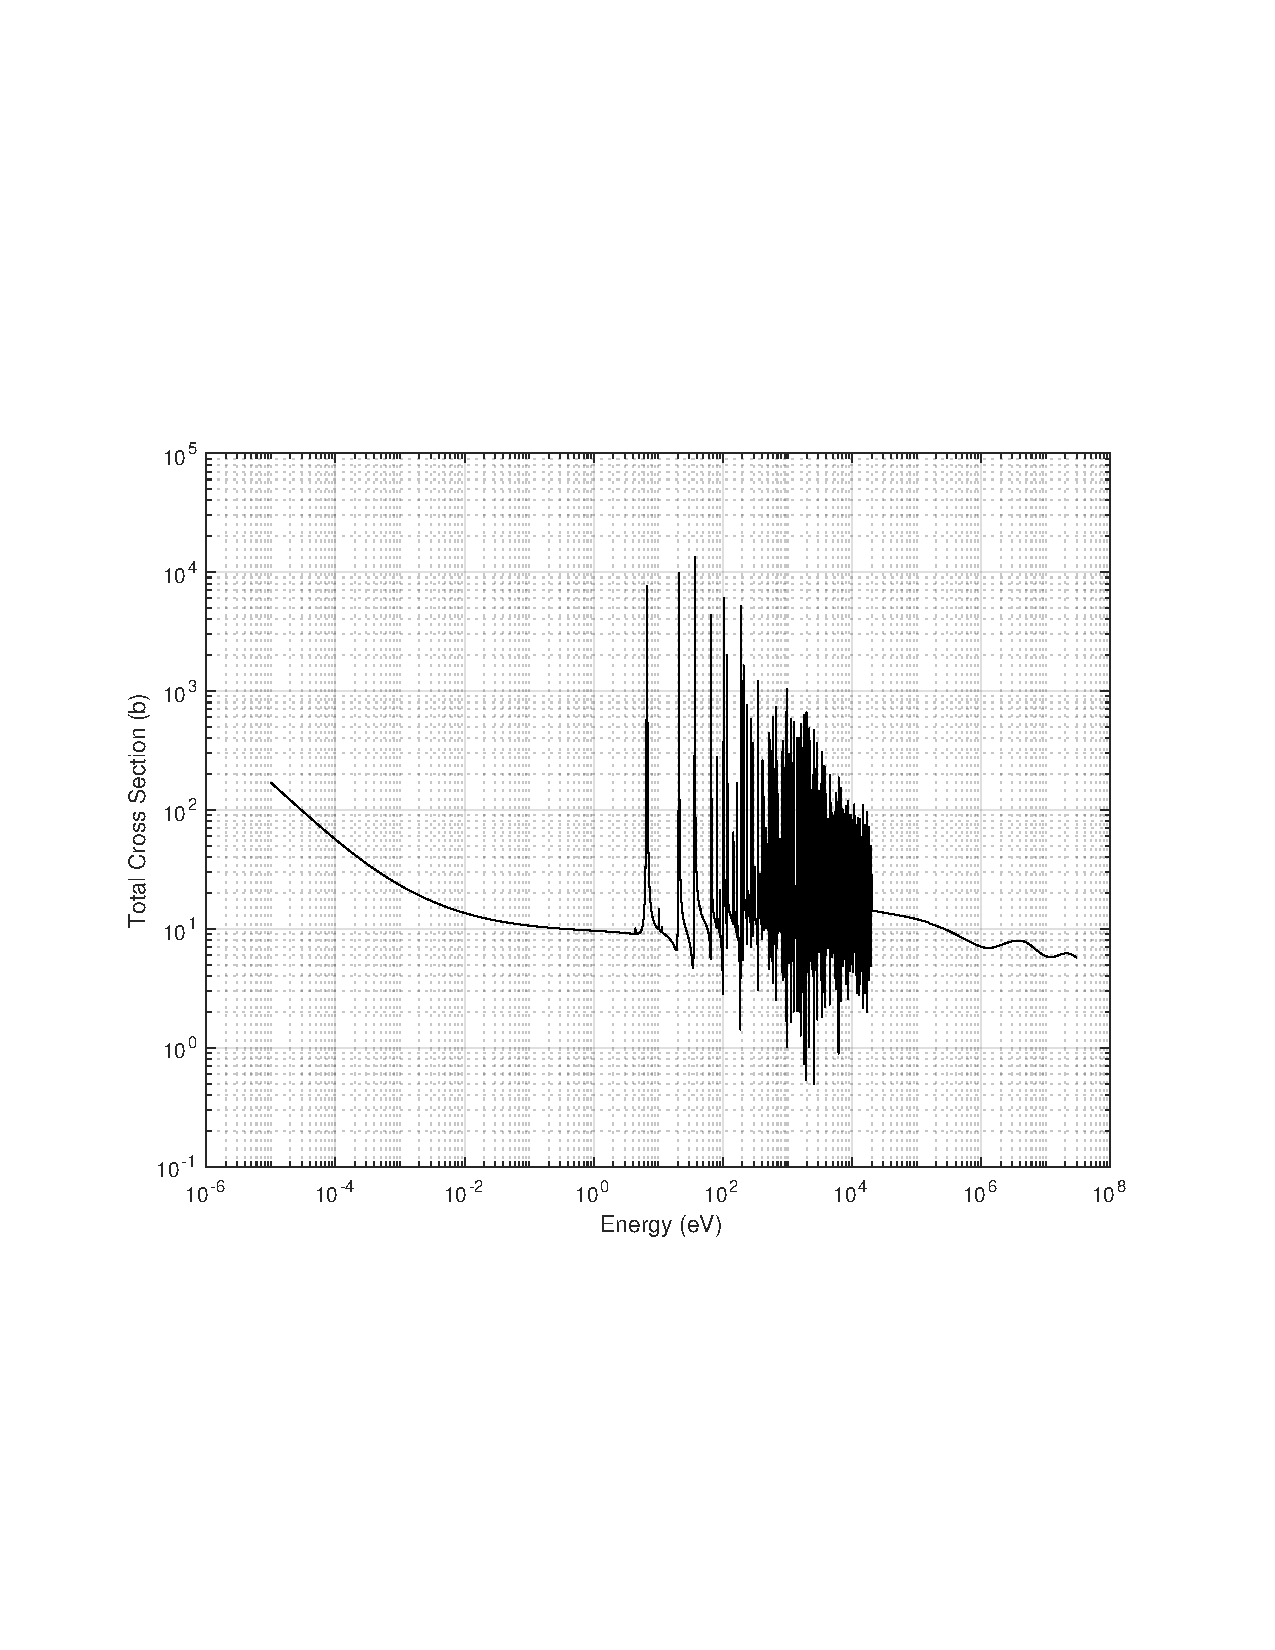
\includegraphics[trim={3.75cm 6.75cm 3.75cm 6.75cm}, width=0.8\textwidth]{./Figures/u238_totalXS_293k.pdf}
\caption{$^{238}$U total cross section at 293~K in ENDF/B-VII.1 processed by NJOY}
\label{Fig:libraryGeneration_u238_totalXS_293K}
\end{center}
\end{figure}

A plot of the $^{238}$U total cross section is given in Fig.~\ref{Fig:libraryGeneration_u238_totalXS_293K} to illustrate these ranges. For this isotope, the thermal range is below a few eV. The resolved resonance range is up until about 20~keV. As we can see, there is much structure. The unresolved resonance range is from 20 to 100~keV. The cross section here appears to be smooth, as only the average or expected cross section is plotted here. In reality, there are resonances that are treated statistically using probability tables, but these are not shown on the plot. The fast region is above 100~keV and is smooth, but contains a few small bumps, primarily because of contributions from higher chance fission.

\subsection{ENDF-6 Format}

If one wants to use nuclear data, they need to be familiar with the ENDF-6 format. Unfortunately, the ENDF format dates back to the 1960s when behemoth computers that were as large as a house that ate punchcards roamed the earth and we have to sadly deal with the cruft that all that legacy entails. Thankfully, it is at least organized and the high level is not all that tricky. As one starts delving into the guts of nuclear data formats, it gets a bit overwhelming. And when one does this long enough, they start speaking an arcane language that sounds like gibberish to the uninitiated listener.

The data formats require specifying the projectile and the target. For the former, we almost always take this as a neutron in reactor physics. For the latter, we need three pieces of information: the charge number $Z$, the mass number $A$, and the isomer state $s$, which is usually the ground state $s = 0$. The charge and mass number are grouped into a single identifier called a ZAID (Z-A ID or more often just pronounced phonetically.) The ZAID is a unique identifier for an isotope given by the following expression:
\begin{align}
  \text{ZAID} = 1000 Z + A .
\end{align}
For example, $^{235}$U is 92235, since $Z = 92$ and $A = 235$.

Once the ZAID is given, we then need to decide which file number within the evaluation to get the data from. This is called the MF number. The most common of these is given in Table~\ref{Table:nuclearData_ENDF_MF}. The most useful of these is MF 3, which stores all of the integral cross sections for every reaction type as a series of points as a function of energy $E$. The MF 2 file contains information about resonance parameters for formulas that are used to create these pointwise cross sections. Information on the differential and double-differential cross sections can be obtained in files 4-6. Of particular note is the fission neutron spectrum $\chi(E)$, which is in MF 5. One odd thing is that the fission multiplicities $\nu$ are in the header, MF 1. Honestly, this feels like a bit of an oversight that got patched in, but as the old saying goes, the less we know about how nuclear data is made the better off we all are.

\begin{table}[htp!]
\caption{Commonly Used ENDF-6 File (MF) Numbers}
\begin{center}
\begin{tabular}{|c|p{12cm}|} \hline
	1	& General Information and Fission Multiplicity Data \\
	2	& Resonance Parameter Information \\
	3	& Cross Sections \\
	4	& Secondary Angular Distributions \\
	5	& Secondary Energy Distributions \\
	6	& Secondary Combined Energy-Angle Distributions \\
	7	& Thermal Scattering Data (see discussion) \\
	8	& Radioactivity and Fission Product Yields \\
	12	& Multiplicities for Photon Production \\
	13	& Cross Sections for Photon Production \\
	14	& Angular Distributions for Photon Production \\
	15	& Energy Distributions for Photon Production \\ \hline
\end{tabular}
\end{center}
\label{Table:nuclearData_ENDF_MF}
\end{table}%

For many of the files, we need to select the reaction type. This is encoded by an MT number. There is little rhyme or reason for how these numbers were handed out, so we just list a few common ones in Table~\eqref{Table:nuclearData_ENDF_MT}.

\begin{table}[htp!]
\caption{Most Relevant ENDF-6 Reaction (MT) Numbers}
\begin{center}
\begin{tabular}{|c|p{12cm}|} \hline
	1	& Total \\
	2	& Elastic Scattering \\
	16	& (n,2n) Multiplicity \\
	18	& Fission \\
	51	& Inelastic Scattering to First Nuclear Level \\
	52	& Inelastic Scattering to Second Nuclear Level \\
	... & \\
	90	& Inelastic Scattering to 40th Nuclear Level \\
	91	& Inelastic Scattering into Continuum \\
	102	& (n,$\gamma$) Radiative Capture \\
	103 & (n,p) Capture \\
	107	& (n,$\alpha$) Capture \\ \hline
\end{tabular}
\end{center}
\label{Table:nuclearData_ENDF_MT}
\end{table}%

Unfortunately, there is a bit of an inconsistency in how thermal scattering law for chemical binding effects is handled. In modern evaluations, these are typically grouped in separate libraries with a file for each particular compound (e.g., hydrogen in light water, carbon in graphite). Typically included are MF types 3 and 7 for the integrated cross section and $S(\alpha,\beta)$ functions. The MT numbers are often a bit arbitrary here. The best strategy here is probably just to look at them all (there are not too many, for better or worse) and just select what we are looking for.

\subsection{JAva-based Nuclear Information Software (JANIS)}

Thankfully, for educational purposes we have easy-to-use tools to access a wide array of the available nuclear data. This means we do not need to concern ourselves with the details of cryptic nuclear data formats. (At least up to the point of doing actual work.) The Nuclear Energy Agency has developed the the JAva-based Nuclear Information Software (JANIS), that supports quick lookups of nuclear data. There are both downloadable and web-based versions available that create both plots as well as tables that can be exported into text files for further processing. Unfortunately, it cannot do everything yet, but is quite powerful and a good way to get oriented or just to do a quick lookup of a cross section. 

The reader is encouraged to play around: \url{https://www.oecd-nea.org/janisweb/}.





%%%%%%%%%%%%%%%%%%%%%%%%%%%%%%%%%%%%%%%%%%%%%%%%%%%%%%%%%%%%%%%%%%%%%%%%%%%%%%%%%%%%%%%%%%%%%%%%%%%%
\section{Point-wise Data Construction}

The ENDF nuclear data files are in formats that are not particularly convenient for use in a reactor analysis. The goal of a nuclear data evaluation is to provide a library that provides a detailed description of the underlying data that accurately describes the physics while keeping storage requirements to a minimum. Because of this, there are a wide number of ways that nuclear data can be represented within ENDF and the evaluator exercises discretion in terms of how this is best done. 

The goal of a nuclear data processing code is to read in the data files and translate it into a usable form. The first step in this process for a cross section is to create a pointwise dataset on an extremely fine grid of energies $E_i$ with corresponding cross section values $\sigma_r^j(E_i)$. In the nomenclature of reactor physics, we often refer to this dataset as a hyperfine library. 

The resolution requirements are defined such that the use of \emph{linear-linear} interpolation will lead to accurate (usually within less than 1\% error) estimation of the cross section over the entire range. The number of datapoints ranges widely depending on the isotope. The simplest isotope, $^1$H can be accurately represented with a few hundred datapoints. On the other extreme, $^{238}$U has a very complicated cross section owing to numerous nuclear resonances, and over $10^5$ energy datapoints are required to accurately represent the cross section. 

Typically the ENDF-6 representation has components spread across two files: File 3 for non-resonance smooth cross sections and File 2 for resonance data and hard-sphere potential scattering. The nuclear data processing code reads both files (if they are present) and produces a cross section that is the sum of the information in these files. We can write the cross section at some energy point $E$ as
\begin{align}
  \sigma(E) = \sigma_\text{smooth}(E) + \sigma_\text{potential}(E) + \sigma_\text{resonance}(E) .
\end{align}
We then take the series of points and assume a linear-linear interpolation to get what is called a pointwise continuous-energy library.

\subsection{Smooth Cross Sections}

A portion of the cross section that is unrelated to the resonances is given in File~3 as point-wise data. Typically, this data are those cross sections that cannot be adequately represented using one of the models for resonance behavior or hard-sphere potential scattering. Most often, this includes the entire unresolved resonance and fast regions as these are above the resonances and a hard-sphere potential model is inadequate to predict the cross section behavior. Depending the evaluation, the rest of the cross section data may or may not be in File 3. In fact, the thermal region can often be reconstructed using resonance parameter data where the ``peak'' occurs at some negative energy value.

\begin{figure}[tb!]
\begin{center}
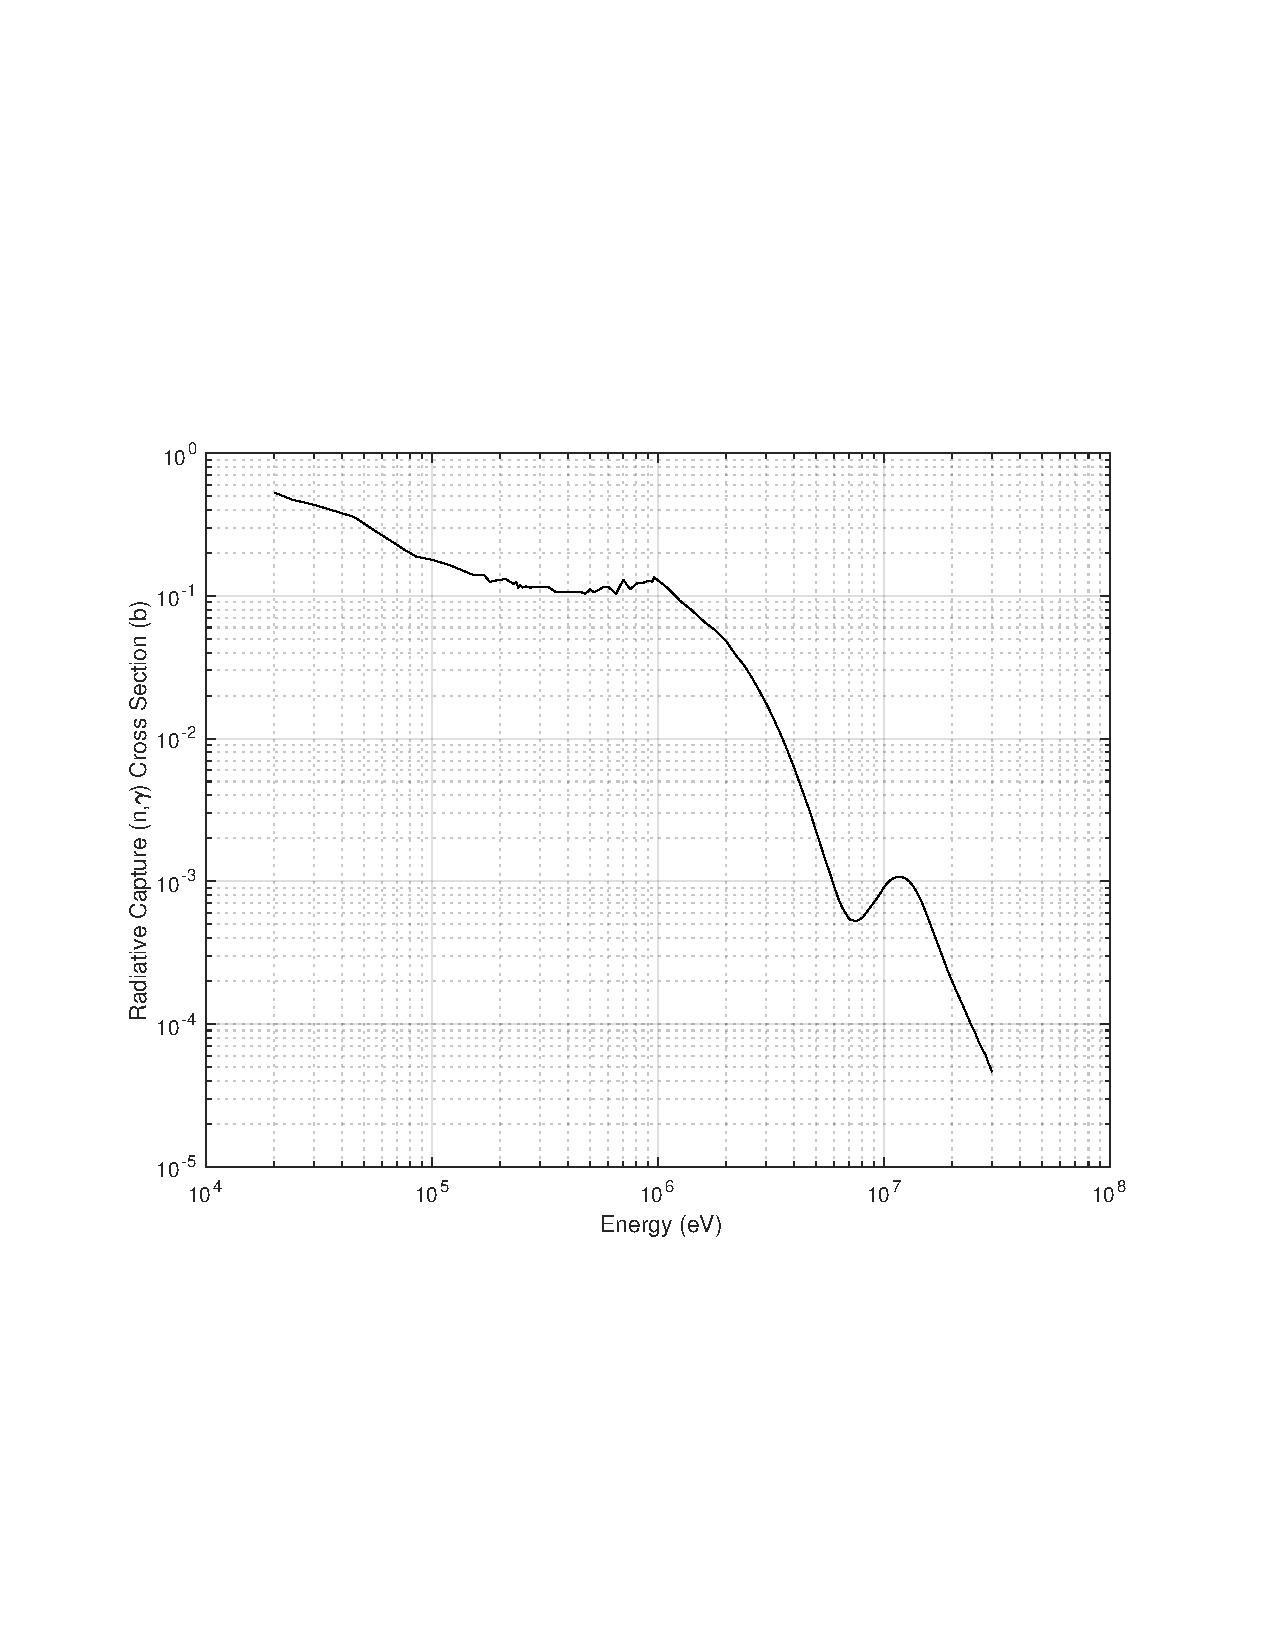
\includegraphics[trim={3.75cm 6.75cm 3.75cm 6.75cm}, width=0.8\textwidth]{./Figures/u238_ngammaXS_mf3.pdf}
\caption{ENDF-6 File 3 $^{238}$U radiative capture (n,$\gamma$) cross section component in ENDF/B-VIII.0}
\label{Fig:libraryGeneration_u238_captureXS_MF3}
\end{center}
\end{figure}

The File 3 contribution of the $^{238}$U radiative capture (n,$\gamma$) cross section is displayed in Fig.~\ref{Fig:libraryGeneration_u238_captureXS_MF3}. Note that this data is zero below 20~keV, which is the boundary between the resolved and unresolved resonance ranges. The information to create the missing data is located in File 2.

\subsection{Hard-Sphere Potential Scattering}

The elastic scattering cross section consists of two components. The first, which is covered in this section, is potential scattering where a neutron scatters off the surface of the nucleus in a billiard-ball like collision. The second part (covered in the next sections) involves the formation of a compound nucleus where a neutron is captured by the nucleus, a neutron is emitted, and the nucleus is left in the ground state.

For low neutron energies, the potential of the nucleus can be approximated as a hard sphere where the neutron wavefunction cannot penetrate into the nucleus. Making this approximation allows for analytical forms for the cross section and provides a compact way to describe this part of the cross section. This information is stored in File 2 of the nuclear dataset.

The fundamental parameter that characterizes potential scattering is the scattering or channel radius $a$, which is proportional to the size of the nucleus. For many nuclei, the channel radius can be approximated by the semi-empirical relationship:
\begin{align}
  a = ( 0.08 + 0.123 A^{1/3} ) \times 10^{-12} \text{ cm}.
\end{align}
Squaring this value gives an area in units of barns. Note that the channel radius can also be given in File 2 as a function of energy $a(E)$ to provide flexibility to accurately describe the scattering cross section.

The incident neutron is characterized by its wave number using the reduced mass of the neutron,
\begin{align}
  k = \frac{ \sqrt{ 2 m_r E }}{ \hbar } = \frac{ \sqrt{ 2 m_n }}{ \hbar }  \left( \frac{A}{A+1} \right) \sqrt{E} ,
\end{align}
where $m_r$ is the reduced neutron mass and $m_n$ is the neutron mass. From this we define a dimensionless parameter as
\begin{align}
  \rho = k a 	\label{Eq:libraryGeneration_rho_ka}
\end{align}
that appears in many of the expressions describing the resonance cross sections.

The incident neutron is described by a plane wave. The nucleus exerts a short-range spherical potential that perturbs the incident neutron wavefunction such that when the outgoing scattered neutron is far from the nucleus, its wavefunction is shifted in phase. This phase shift described by a set of energy-dependent angles $\varphi_\ell(E)$, where $\ell$ denotes the discrete orbital angular momentum values. The potential scattering cross section can be written as a linear combination of the phase shifts from the different angular momenta values as
\begin{align}
  \sigma_p(E) = \sum_{\ell = 0}^\infty ( 2 \ell + 1 ) \frac{4\pi}{k^2} \sin^2 \varphi_\ell .
\end{align}
For energies in the range for which the hard-sphere potential is valid (below a few tens of keV typically) we can describe the cross section with only a few phase shift terms. The four of these are
\begin{subequations}
\begin{align}
  \varphi_0 &= \rho, \\
  \varphi_1 &= \rho - \tan^{-1}\rho , \\
  \varphi_2 &= \rho - \tan^{-1}\left( \frac{3\rho}{ 3 - \rho^2 } \right) , \\  
  \varphi_3 &= \rho - \tan^{-1}\left( \frac{\rho (15 - \rho^2 ) }{ 15 - 6 \rho^2 } \right) .
\end{align}
\end{subequations}
(Note there is a typo on $\varphi_3$ in the 2018 version of the ENDF-6 formats manual.)

An important result is for the low-energy neutron case. In this regime, the $\ell = 0$ term of the potential scattering cross section dominates and $\varphi_0 = \rho$. Furthermore the wave number $k$ is small so $\rho$ is small so we can use the small-angle approximation $\sin\rho \approx \rho$. Therefore,
\begin{align}
  \sigma_p \approx \frac{4\pi}{k^2} \sin^2 \rho \approx \frac{4\pi}{k^2} \rho^2 = \frac{4\pi}{k^2} ( ka )^2 = 4\pi a^2 .
\end{align}
We see that at low energies, the potential scattering cross section converges to a constant value. 

This constant potential scattering approximation is often used in many of the analytical expressions involving resonances and is suitable for low-lying resonances found in isotopes such as $^{238}$U. Note that this cross-sectional area corresponds to the surface area of a spherical nucleus. This may seem weird in the context of a cross-sectional area of sphere, which classically would be $\pi a^2$. This seeming inconsistency is because of the wavelike behavior of the neutron at low energies. The neutron is not a point-like particle at this length scale and as wave, it ``feels'' its way around the entire nucleus and experiences its entire area.

\subsection{Single-Level Breit-Wigner Resonance Model}

The ENDF-6 format allows for resonances to be defined in File 2 using different formats. The most commonly used ones are:
\begin{enumerate}
  \item Single-Level Breit-Wigner,
  \item Multi-Level Breit-Wigner,
  \item Reich-Moore,
  \item R-Matrix Limited.
\end{enumerate}

Of these, the single-level Breit-Wigner form is the most simple, but least accurate, as it is only able to account for a single channel. Most resonances of the major actinides are described using the Reich-Moore formulation. For reasons of pedagogical expediency, we only discuss the single-level Breit-Wigner form and direct interested readers to Appendix D of the ENDF-6 Format Manual for information on the others. 

In the single-level Breit-Wigner format resonances are characterized using a set of parameters:
\begin{align}
  \ell 		&= \text{ orbital angular momentum of the resonance excited state.} \nonumber \\
  I    		&= \text{ spin (angular momentum) of the target nucleus.} \nonumber \\
  J			&= \text{ spin state of the resonance for the compound nucleus.} \nonumber \\
  g_J		&= (2J + 1)/[2(2I+1)] = \text{ statistical spin factor.} \nonumber \\
  E_r		&= \text{ peak energy of the $r$th resonance.} \nonumber \\
  \Gamma_{nr}(|E_r|) &= \text{ neutron (elastic scattering) line width for the $r$th resonance at energy $E_r$.} \nonumber \\
  \Gamma_{\gamma r}  &= \text{ radiative capture (n,$\gamma$) line width for the $r$th resonance.} \nonumber \\
  \Gamma_{fr} 		 &= \text{ fission (n,f) line width for the $r$th resonance.} \nonumber \\
  \Gamma_r(|E_r|)	 &= \Gamma_{nr}(|E_r|) + \Gamma_{\gamma r} + \Gamma_{fr} = \text{ total line width for $r$th resonance.} \nonumber
\end{align} 

The neutron line width is a function of energy, whereas the radiative capture and fission are not. The file gives the resonance width at \emph{absolute value} of the resonance peak energy $E_r$. This is important because there can be negative energy resonances, which correspond to bound states within the compound nucleus that are classically inaccessible because even a neutron with zero kinetic energy forming that compound nucleus would put it into an excited state with an energy above those states. While these states are classically inaccessible, the fact that the energy state is indeterminate from quantum mechanics means there is still a contribution to the cross section at positive energies from these bound state resonances.

The energy-dependence of the neutron line width is because the neutron penetrates a certain depth into the nucleus and the amount of penetration is a function of kinetic energy and the orbital angular momentum state of the resonance. This is
\begin{align}
  \Gamma_{nr}(E) = \frac{\Pi_\ell(E)}{\Pi_\ell(|E_r|)} \Gamma_{nr}(|E_r|) .
\end{align}
Here $\Pi_\ell$ are the penetrability factors, which are
\begin{subequations}
\begin{align}
  \Pi_0 &= \rho, \\
  \Pi_1 &= \frac{\rho^3}{1 + \rho^2}, \\
  \Pi_2 &= \frac{\rho^5}{9 + 3\rho^2 + \rho^4}, \\  
  \Pi_3 &= \frac{\rho^7}{225 + 45\rho^2 + 6\rho^4 + \rho^6}.
\end{align}
\end{subequations}
Here $\rho$ is given by Eq.~\eqref{Eq:libraryGeneration_rho_ka}, which depends on energy by way of the wavenumber. Note that the penetrability factors are more often described with the variable $P_\ell$, but we change this here so as not to confuse them with the Legendre polynomials.

For angular momenta $\ell > 0$, the effective peak of the resonance is given by $E_r'$, which is itself a function of energy by way of the shift factors $S_\ell$. This is
\begin{align}
  E_r'(E) = E_r + \frac{ S_\ell(|E_r|) - S_\ell(E) }{ 2 \Pi_\ell(|E_r|) } \Gamma_{nr}(|E_r|).
\end{align}
The shift factors are
\begin{subequations}
\begin{align}
  S_0 &= 0, \\
  S_1 &= -\frac{1}{1 + \rho^2}, \\
  S_2 &= -\frac{18 + 3\rho^2}{9 + 3\rho^2 + \rho^4}, \\  
  S_3 &= -\frac{675 + 90 \rho^2 + 6 \rho^4 }{225 + 45\rho^2 + 6\rho^4 + \rho^6}.
\end{align}
\end{subequations}

We can now proceed with giving the resonance cross section formulas. These are taken for a target at rest or zero temperature. Normally these would then be adjusted for the actual temperature in a process called Doppler broadening that we discuss in the next section.

The absorption (with radiative capture and fission being the most relevant) resonances are simpler than scattering, so we discuss these first. The contribution from the resonances for these reactions are
\begin{align}
  \sigma_x(E) = \frac{4\pi}{k^2} \sum_{\ell = 0}^L \sum_J g_J \sum_{r = 1}^{N_J} \frac{ \Gamma_{nr} \Gamma_{xr} }{ 4 ( E - E_r' )^2 + \Gamma_r^2 } , \quad x \in \gamma, f.
\end{align} 
The energy dependencies of the quantities $\Gamma_{nr}$ $\Gamma_r$, and $E_r'$ are omitted for brevity. In ENDF-6 File 2, the resonances are given as pairs of $\ell$ and $J$ values, so effectively we end up summing over all resonances in the file and using the appropriate definitions.

The elastic scattering resonance cross section includes two terms. The first is similar to that of absorption and accounts for compound nucleus formation. The second term is because of interference between compound nucleus formation and potential scattering. This arises because each event has an associated wavefunction that must be squared (multiplied by complex conjugate) to get the cross section and the interference term is the cross term from that operation. The resulting expression for the resonance cross sections are
\begin{align}
  \sigma_s(E) = \frac{4\pi}{k^2} \sum_{\ell = 0}^L \sum_J g_J \sum_{r = 1}^{N_J} \frac{ \Gamma_{nr}^2 - 2 \Gamma_r \Gamma_{nr} \sin^2\varphi_\ell + 2 (E - E_r' ) \Gamma_{nr} \sin(2\varphi_\ell) }{ 4 ( E - E_r' )^2 + \Gamma_r^2 } .
\end{align} 
Note again that the energy dependencies of the quantities $\Gamma_{nr}$ $\Gamma_r$, $\varphi_\ell$, and $E_r'$ are omitted.

The resonance contribution to the total cross section is the sum of the radiative capture, fission, and elastic scattering components.

\subsection{Pointwise Construction Algorithm}

The task is to construct an approximate pointwise representation of the continuous-energy cross section subject to interpolation schemes between the energy grid points. For neutron cross sections, we typically use linear-linear interpolation between the energy $E$ and the cross section $\sigma(E)$. Given a set of energies $E_i$ and cross sections $\sigma(E_i) = \sigma_i$, we have an approximate interpolated cross section of
\begin{align}
  \widetilde{\sigma}(E) = \sigma_i + \frac{ E - E_i }{ E_{i+1} - E_i } ( \sigma_{i+1} - \sigma_i ) .
\end{align}

Other interpolation schemes are possible. For example, photon libraries use typically logarithmic interpolation schemes, which are to be more appropriate for photons given the energy dependence of the cross sections. Going back to neutrons, one might be tempted to use higher-order polynomials to approximate the cross section such as cubic splines. Usually this is not done because it would complicate the interpolation. For cubic splines this would involve some numerical root finding scheme every time a cross section needs to be interpolated, which would drive up the expense of many downstream calculations. Second, the functional form of resonances means that while we would reduce the number of points going to higher-order polynomials, it would not actually save us all that much to justify the downstream burdens. Therefore, this motivates us to stick with piecewise linear cross sections.

To find an appropriate energy grid, we need to select a set of points that meets some global error tolerance $\epsilon$ such that the relative error in the interpolated cross section versus the actual cross section is less than epsilon,
\begin{align}
  \frac{ | \widetilde{\sigma}(E) - \sigma(E) | }{ \sigma(E) } \le \epsilon ,
\end{align}
for all energies $E$. Guaranteeing this for every energy is very difficult, so we often relax this using a method of bisection.

The first step in the bisection method is to start with a set of essential energy points. These essential points usually include:
\begin{enumerate}
  \item The energy points specified in the smooth cross section in File 3,
  \item The resonance peaks $E_r$ specified in file 2,
  \item Reaction thresholds for inelastic scattering or other threshold reactions,
  \item The minimum, maximum, energy group boundary points, and any others specified by the end user.
\end{enumerate}
The reason for the File 3 points is these were already chosen by the nuclear data evaluator to be the best set of points to most efficiently describe the cross section and removing them may introduce additional errors. The resonance peak energies $E_r$ represent places where the cross section experiences a sharp changes and excluding these points could mean that the algorithm could miss an entire resonance, which would lead to major errors in a downstream calculation. The third set is essential to ensure we preserve reaction thresholds lest we could have unphysical behavior. For the fourth, these represent points the user explicitly wants to have an accurate cross section or should exist in the library for the purpose of convenience, such as energy group boundaries.

We now proceed to loop over the energy grid points. Suppose we are at energy grid point $i$, we compute the midpoint energy $E_{mid} = (E_i + E_{i+1} )/2$ and then compute the exact cross section at $E_{mid}$ and the approximation using linear-linear interpolation. If these values are \emph{not} within a relative error tolerance $\epsilon$, we add $E_{mid}$ to the energy grid and reindex the energy grid points such that $E_{i+1} \rightarrow E_{mid}, E_{i+2} \rightarrow E_i$, and so on. We then repeat the process, computing a new value of $E_{mid}$, evaluating the cross sections and inserting points as needed until we achieve a fine enough resolution to meet the error tolerance, at which point we move onto the next energy grid point and bisect for that range. This process continues until we reach the end of the energy grid structure.

This discussion assumes we do this for every cross section independently. This leads to the complication of having different energy grids for every reaction cross section and every isotope. One extreme is to use a unionized energy grid for every isotope and every reaction. This leads to exceptionally large files and is usually not done. The usual compromise is to use the same energy grid for all reactions of the same isotopes with different energy grids for different isotopes. (The exception here is threshold reactions, which are zero below a certain energy and these zeros are usually not stored explicitly.)

This modifies the algorithm slightly in that we do the bisection simultaneously for all reactions within an isotope and we test that all the cross sections for all reactions are within the relative error tolerance. If any one of them fails, we add another point to the grid.

The final point here relates to the total cross section or any others that are the sum of a series of partials (e.g., absorption or inelastic). Usually it is best to perfrom the pointwise construction on all of the individual reaction cross sections. All combined cross sections such as the total cross section are then computed as the sum of the partials. In this manner, we guarantee that the cross sections add together correctly.

%%%%%%%%%%%%%%%%%%%%%%%%%%%%%%%%%%%%%%%%%%%%%%%%%%%%%%%%%%%%%%%%%%%%%%%%%%%%%%%%%%%%%%%%%%%%%%%%%%%%
\section{Doppler Broadening}

The smooth cross sections from File 3 and those constructed from resonance parameters given in File 2 are taken to be for a target at rest or zero temperature. Of course, any actual system will be at a finite temperature and this has a major effect on the microscopic cross sections. The reason is that the background nuclei experience random thermal motion and therefore the neutrons encounter these nuclei at different relative velocities or energies. The cross section of any individual interaction is taken at this relative energy. Since we cannot know the precise velocity of the target nuclei in every collision, we need to average over all possible nuclear velocities in a process called thermal averaging or more often Doppler broadening.

The most pronounced impact on the cross sections occur near the resonances. Recall the cross section near a resonance is a highly peaked function and the effect of Doppler broadening is to smooth this peak out, broadening the resonance. The higher the temperature, the more broadening that occurs. This means that the resonance impacts a large range of energies and neutrons are more likely to interact with the resonance. In light-water reactors with low-enriched uranium fuel, the Doppler broadening of the $^{238}$U resonances leads to a significant increase in the amount of absorption from them. This Doppler effect is one of the most important physical mechanisms that need to get resolved correctly to get the right reaction rates and therefore criticality.

\subsection{Maxwell-Boltzmann Distribution}

The velocities of particles in thermodynamic equilibrium are described by a Maxwell-Boltzmann distribution. The velocity in each independent direction $(V_x,V_y,V_z)$ is described by a normal distribution. The distribution for the speed can then be written as
\begin{align}
  M(\mathbf{V},T) dV_x dV_y dV_z 
  = \left( \frac{ A m_n }{ 2 \pi k_B T } \right)^{3/2} \exp \left( -\frac{ A m_n V^2 }{ 2 k_B T } \right) dV_x dV_y dV_z
\end{align}
where the speed is
\begin{align}
  V = \sqrt{ V_x^2 + V_y^2 + V_z^2 } .
\end{align}
This can expressed in spherical coordinates in terms of the speed $V$ as
\begin{align}
  M(V,\mu,\gamma,T) dV d\mu d\gamma &= \frac{1}{4\pi} M(V,T) dV d\mu d\gamma \nonumber \\
  &= \left( \frac{Am_n}{2\pi k_B T} \right)^{3/2} \exp \left( -\frac{ A m_n V^2 }{ 2 k_B T } \right) V^2 dV d\mu d\gamma.
\end{align}
Here $V^2 dV d\mu d\gamma$ is a 3-D differential velocity element analogous to a differential volume element. Here $\mu$ is the cosine of the angle between the nucleus an arbitrary polar axis, which is usually chosen as the incident neutron direction, and $\gamma$ is the azimuthal angle about that axis.

We then define
\begin{align}
  \beta = \frac{A m_n}{ 2 k_B T },
\end{align}
giving
\begin{align}
  M(V,\mu,\gamma,T) dV d\mu d\gamma = \left( \frac{\beta}{\pi} \right)^{3/2} e^{-\beta V^2} V^2 dV d\mu d\gamma.
\end{align}

From here we can work out the integrals and show that this distribution is normalized such that
\begin{align}
  \int_0^{2\pi} \int_{-1}^1 \int_0^\infty  M(V,\mu,\gamma,T) dV d\mu d\gamma = \int_0^\infty M(V,T) dV = 1.
\end{align}
This normalization will become important to conserve particles in collisions.

This distribution can be transformed to be in terms of the kinetic energy of the nucleus. Performing the variable transformation,
\begin{align}
  E &= \frac{1}{2} A m_n V^2, \nonumber \\
  dE &= A m_n V dV . \nonumber
\end{align}
and integrating out the $\mu$ and $\gamma$ variables gives
\begin{align}
  M(E,T) dE 
  = &\frac{2}{\sqrt{\pi} k_B T} \sqrt{ \frac{A E}{k_B T} } \exp \left( -\frac{ AE }{ k_B T } \right) dE.
\end{align}

We assume that the velocities of the background nuclei are distributed approximately with the Maxwell-Boltzmann distribution. In reality, in a solid, for example, the velocities in some directions could be inhibited by chemical bonds. Fortunately, for temperatures that are not too low, those well in excess of the Debye temperature, the assumption is a very good one. This applies for most materials we encounter in reactor analysis for room temperature and above.

\subsection{Thermal Averaging of Cross Sections}

If we average over all possible nuclear velocities for a media with temperature $T$, we get a reaction rate per incident neutron with speed $v$ of
\begin{align}
  R(v) = v \sigma(v,T) = \int_0^{2\pi} \int_{-1}^1 \int_0^\infty v_{rel} \sigma(v_{rel},0) M(V,T) dV d\mu d\gamma . 
\end{align}
Here we suppressed the reaction-type index on the cross section. The variable $v_{rel}$ is the relative speed between the incident neutron and the target nucleus. Using the law of cosines, we can write the relative speed as
\begin{align}
  v_{rel} = \sqrt{ v^2 + V^2 - 2 v V \mu } .
\end{align}
Since this is independent of the azimuthal angle $\gamma$ and nothing else in the integral is as well, we can simply carry out that integration to get
\begin{align}
  R(v) = v \sigma(v,T) = \frac{1}{2} \int_{-1}^1 \int_0^\infty v_{rel} \sigma(v_{rel},0) M(V,T) dV d\mu  . \label{Eq:libraryGeneration_thermalAverageReactionRate_azimuthallyIntegrated}
\end{align}

The presence of $\mu$ in the $v_{rel}$ and therefore the zero-temperature cross section $\sigma(v_{rel},0)$ is problematic from doing this integral. It turns out that the problem is easier if instead we integrate over the relative speed using a variable transformation between $\mu$ and $v_{rel}$. By differentiating the relative speed with respect to $\mu$ we obtain
\begin{align}
  d\mu = -\frac{v_{rel}}{v V} dv_{rel} .
\end{align}

The limits of integration are a bit tricky to work out. First, $\mu$ has the range $[-1,1]$, but it is under a square root, so we must be careful. Second, the minus sign from the transformation flips the limits of integration. 

The $\mu = -1$ case (upper limit after the flip) is straightforward, giving $v_{rel} = \sqrt{(v+V)^2} = V + v$, discarding the nonphysical negative sign. This gives the range $v_{rel} < V + v$.

\begin{figure}[tb!]
\begin{center}
\begin{center}
\begin{tikzpicture}
  \draw[-latex,thick] (0,0) -- (0,11);
  \draw[-latex,thick] (0,0) -- (11,0);
  \node at (10.75,-0.25) {$V$};
  \node at (-0.325,10.75) {$v_{rel}$};
  
  \draw[line width=0.5mm,blue] (0,4) -- (7,11);
  \draw[line width=0.5mm,blue] (4,0) -- (11,7);
  \draw[line width=0.5mm,blue] (0,4) -- (4,0);
  
  \filldraw[blue!40, opacity=0.4, decoration={random steps,segment length=0.2cm}] (4,0) -- (0,4) -- (7,11) decorate{-- (11,7)} -- cycle;
  
  \node[rotate =  45] at (7.5,3) {$v_{rel} = V - v$};
  \node[rotate =  45] at (3,7.5) {$v_{rel} = V + v$};
  \node[rotate = -45] at (1.75,1.75) {$v_{rel} = v - V$};
\end{tikzpicture}
\end{center}
\caption{Integration range for thermally averaged reaction rate}
\label{Fig:libraryGeneration_thermalAveragingIntegrationRange}
\end{center}
\end{figure}

The case of $\mu = 1$ (lower limit after the flip) yields $v_{rel} = \sqrt{(v - V)^2} = \pm ( v - V )$. There are two potentially physically meaningful solutions: $v - V$ when $v > V$ and $V - v$ when $v < V$. This implies the respective ranges of $v_{rel} > v - V$ and $v_{rel} > V - v$. Taking the intersection of these three ranges yields the integration range depicted in Fig.~\ref{Fig:libraryGeneration_thermalAveragingIntegrationRange}.

These integration ranges can be written compactly using the absolute value
\begin{align}
  R(v) = v \sigma(v,T) = \frac{1}{2 v} \int_0^\infty v_{rel}^2 \sigma(v_{rel},0) \int_{|v-v_{rel}|}^{|v+v_{rel}|} \frac{1}{V} M(V,T) dV dv_{rel}  .
\end{align}
We can then carry out the inner integral over the target speed $V$. The result in terms of the incident neutron speed $v$ and relative speed between it and the target nucleus $v_{rel}$ is then
\begin{align}
  R(v) = v \sigma(v,T) = \frac{1}{v} \sqrt{ \frac{\beta}{\pi} } \int_0^\infty v_{rel}^2 \sigma(v_{rel},0) \left[ e^{-\beta ( v - v_{rel} )^2} -  e^{-\beta ( v + v_{rel} )^2} \right] dv_{rel}  .
\end{align}

We can then cast this to be in terms of the neutron energy. We define the relative kinetic energy experienced by the target nucleus as
\begin{align}
  E_{rel} = \frac{1}{2} m_n v_{rel}^2 . \nonumber
\end{align}
We then obtain the thermally averaged cross section as
\begin{align}
   \sigma(E,T) &= \frac{1}{2 E} \sqrt{ \frac{\alpha}{\pi} } \int_0^\infty \sqrt{E_{rel}} \sigma(E_{rel},0) \nonumber \\ &\times \left[ \exp\left( -\alpha \left( \sqrt{E} - \sqrt{E_{rel}} \right)^2 \right) -  \exp\left( -\alpha \left( \sqrt{E} + \sqrt{E_{rel}} \right)^2 \right) \right] dE_{rel}  \label{Eq:libraryGeneration_thermalAveragedXS_energy}
\end{align}
where
\begin{align}
  \alpha = \frac{A}{k_B T} .
\end{align}
(This $\alpha$ is different than the scattering ratio.)

From here we need to know the functional form of the cross section. There are two cases that appear commonly and can actually be worked out analytically. 

The first is the case of a $1/v$ absorber. To solve this, it is actually easier to use Eq.~\eqref{Eq:libraryGeneration_thermalAverageReactionRate_azimuthallyIntegrated} directly:
\begin{align}
  \sigma(v,T) = \frac{1}{2v} \int_{-1}^1 \int_0^\infty v_{rel} \left( \frac{1}{v_{rel}} \right)  M(V,T) dV d\mu  = \frac{1}{v}  \int_0^\infty  M(V,T) dV = \frac{1}{v} .
\end{align}
Here we recall that the Maxwell-Boltzmann distribution $M(V,T)$ is normalized such that integrating over all target speeds yields one. This result says that a $1/v$ cross section is unaffected by thermal motion.

The second case is constant (hard-sphere) potential scattering $\sigma(v_{rel},0) = \sigma_p$. For this we can work out the integral of the final result directly to obtain
\begin{align}
  \sigma(E,T) = \sigma_p \left[  \left( 1 + \frac{ k_B T }{ 2 A E } \right) \erf \left( \sqrt{\frac{AE}{k_B T}} \right) + \sqrt{ \frac{ k_B T }{ \pi A E } } \exp \left( -\frac{AE}{k_B T} \right) \right]. \label{Eq:libraryGeneration_FreeGasScatteringXS}
\end{align}
We see that the potential scattering cross section gets corrected by an energy-dependent factor involving familiar exponentials and perhaps a less familiar function called the \emph{error function}. The error function was first studied in the domain of statistical inference, which led to its name. Unfortunately, even through neutron interactions have little to do with the topic, we are stuck with the name. The error function is defined by the following integral:
\begin{align}
   \text{erf}(x) = \frac{2}{\sqrt{\pi}} \int_0^x e^{-t^2}  dt .
\end{align}
This is available in any standard mathematics library.

The above expression is not particularly intuitive, but the limiting behavior for low and high energies is insightful. At low energies, the error function goes to zero and its factor diverges. Using L'Hopital's rule, we can show that this term limits to a constant value. The second term, on the other hand, diverges because the exponential tends toward one while the $1/\sqrt{E}$ factor diverges. Because this is equivalent to inverse speed and the constant becomes small for small speed $v$, we can assert that:
\begin{subequations}
\begin{align}
  \sigma_s(E,T) = \sqrt{ \frac{ k_B T }{ \pi A }  } \frac{\sigma_p}{v}, \quad E \ll k_B T.
\end{align}
The behavior of the scattering cross at low energies exhibits the same trend as capture cross sections.

At high energies, the both the error function term and its factor converges to one. The exponential term tends toward zero. Therefore, for high energies, we can state
\begin{align}
  \sigma_s(E,T) = \sigma_s(E) = \sigma_p, \quad E \gg k_B T .
\end{align}
\end{subequations}
It is often acceptable to make this assumption in the resonance region, which simplifies the analysis in reactor physics calculations.

It is also possible to develop approximate, semi-analytical expressions for the single-level Breit-Wigner form of the cross section for $\ell = 0$ resonances in terms of the $\psi$ and $\chi$ functions called the \emph{Bethe-Placzek cross sections}. Because these expressions are quite limited in their applicability, we will not go through the entire derivation, which is given in many other reactor physics texts (see Bell \& Glasstone). Nonetheless, they are still useful because they can serve as a check on the more general method for Doppler broadening discussed in the next section.

The Bethe-Placzek absorption cross section for a single resonance $r$ is
\begin{align}
  \sigma_{zr}(E,T) = \sigma_0 \frac{\Gamma_{zr}}{\Gamma_r} \sqrt{ \frac{E_0}{E} } \psi(\zeta,x) , \quad z \in \gamma,f
\end{align}
where the $\psi$ function is
\begin{align}
  \psi(\zeta,x) = \frac{\zeta}{2\sqrt{\pi}} \int_{-\infty}^\infty \frac{1}{1+y^2} \exp \left( -\frac{\zeta^2}{4} ( x - y )^2 \right) dy , \label{Eq:nuclearData_DopplerBroadening_psi}
\end{align}
and the quantity $\sigma_0$ is a cross section given by
\begin{align}
  \sigma_0 = 4\pi \lambdabar_0 g_J \frac{ \Gamma_{nr}(|E_r|) }{ \Gamma_r(|E_r|) } ,
\end{align}
with dimensionless energy
\begin{align}
  x = \frac{2}{\Gamma_r(|E_r|)} ( E - E_r )
\end{align}
and $\lambdabar_0$ being the reduced wavelength of a neutron with a speed corresponding to energy $E_r$,
\begin{align}
  \lambdabar_0 = \frac{A+1}{A} \frac{\hbar}{ m_n v(|E_r|) }  .
\end{align} 
The $\psi$ function needs to be evaluated using numerical integration.

The corresponding Bethe-Placzek scattering cross section is
\begin{align}
  \sigma_s(E,T) = \sigma_p + \sigma_0 \frac{\Gamma_n}{\Gamma} \psi(\zeta,x) + \sigma_0 \frac{a}{\lambdabar} \chi(\zeta,x) ,
\end{align}
where this new function $\chi(\zeta,x)$ can be found using numerical integration:
\begin{align}
  \chi(\zeta,x) = \frac{\zeta}{\sqrt{\pi}} \int_{-\infty}^\infty \frac{y}{1+y^2} \exp \left( -\frac{\zeta^2}{4} ( x - y )^2 \right) dy
\end{align}

\subsection{Doppler Broadening of Piecewise-Linear Cross Sections}

A cross section library is typically represented using a piecewise-linear representation with a resolution chosen to accurately represent the underlying cross section's energy dependence. The goal is to perform Doppler broadening given this piecewise-linear representation at zero temperature as input where the output is another piecewise-linear representation of the Doppler broadened cross section. This can be done exactly using a method often called SIGMA1, which is named after the original code developed by Cullen in the 1970s.

We begin with Eq.~\eqref{Eq:libraryGeneration_thermalAveragedXS_energy} and introduce the following transformation variables:
\begin{subequations}
\begin{align}
  y^2 &= \beta v^2 = \alpha E \\*
  x^2 &= \beta v_{rel}^2 = \alpha E_{rel} .
\end{align}
\end{subequations}
Inserting these gives
\begin{align}
  \sigma(y,T) &= \frac{1}{y^2 \sqrt{\pi}} \int_0^\infty x^2 \sigma(x,0) \left[ e^{-(x-y)^2} - e^{-(x+y)^2} \right] dx.
\end{align}
We define the function
\begin{align}
  \eta(y,T) &= \frac{1}{y^2 \sqrt{\pi}} \int_0^\infty x^2 \sigma(x,0) e^{-(x-y)^2} dx,
\end{align}
which implies the Doppler broadened cross section can be expressed as
\begin{align}
  \sigma(y,T) = \eta(y,T) - \eta(-y,T) .
\end{align}

The cross section is given as a piecewise linear function in energy with cross sections given at grid points $k$ of $\sigma_k$ at energy $E_k$ and $\sigma_{k+1}$ at energy $E_{k+1}$. Transforming into $x$, we can write the cross section as a quadratic function,
\begin{align}
  \sigma(x,0) = A_k + C_k x^2, \quad x \in [x_k,x_{k+1}) .
\end{align}
where $C_k$ is the slope
\begin{align}
  C_k = \frac{ \sigma_{k+1} - \sigma_k }{ x_{k+1}^2 - x_k^2 } \nonumber
\end{align}
and $A_k$ is the intercept that can be found by solving
\begin{align}
  A_k = \sigma_k - C_k x_k^2 . \nonumber
\end{align}

We then insert the piecewise-linear form of the cross section into the expression for $\eta$ to get
\begin{align}
  \eta(y,T) &= \frac{1}{y^2 \sqrt{\pi}} \sum_k \int_{x_k}^{x_{k+1}} x^2 \left( A_k + C_k x^2 \right) e^{-(x-y)^2} dx ,
\end{align}
We then introduce the transformation
\begin{align}
  z = x-y \nonumber
\end{align}
to obtain
\begin{align}
  \eta(y,T) 
  &= \frac{1}{y^2 \sqrt{\pi}} \sum_k \int_{x_k-y}^{x_{k+1}-y} (z+y)^2 \left( A_k + C_k (z+y)^2 \right) e^{-z^2} dz \nonumber \\
  &= \frac{1}{y^2 \sqrt{\pi}} \sum_k \int_{x_k-y}^{x_{k+1}-y} ( z^2 + 2zy + y^2 ) \left[ A_k + C_k ( z^2 + 2zy + y^2 ) \right] e^{-z^2} dz \nonumber \\
  &= \frac{1}{y^2 \sqrt{\pi}} \sum_k \int_{x_k-y}^{x_{k+1}-y} \bigg[ C_k z^4 + 4 C_k y z^3 + ( A_k + 6 C_k y^2 ) z^2  \nonumber \\
  &\hspace{2.5cm}  + ( 2 A_k y + 4 C_k y^3 ) z + ( A_k y^2 + C_k y^4 )  \bigg] e^{-z^2} dz
\end{align}

This expression can be evaluated analytically by defining
\begin{subequations}
\begin{align}
  F_n(a)   &= \frac{2}{\sqrt{\pi}} \int_0^a z^n e^{-z^2} dz , \\
  H_n(a,b) &= F_n(b) - F_n(a) .
\end{align}
\end{subequations}
The $F_n$ functions can be carried out analytically as
\begin{subequations}
\begin{align}
  F_0(a) &= \erf(a) , \\
  F_1(a) &= \frac{1}{\sqrt{\pi}} \left( 1 - e^{-a^2} \right), \\
  F_2(a) &= \frac{1}{2} \erf(a) - \frac{a}{\sqrt{\pi}} e^{-a^2} , \\
  F_3(a) &= \frac{1}{\sqrt{\pi}} \left[ 1 - ( 1 + a^2 ) e^{-a^2} \right] , \\
  F_4(a) &= \frac{3}{4} \erf(a) - \frac{1}{\sqrt{\pi}} \left( a^3 + \frac{3a}{2} \right) e^{-a^2} .
\end{align}
\end{subequations}


The algorithm can be generalized to broaden any library from temperature $T_1$ to a \emph{higher} temperature $T_2$. The only changes in the algorithm replaces $\sigma(x,0)$ with $\sigma(x,T_1)$ in the integrand and the temperatures in the parameters $\beta$ and $\alpha$ become $\Delta T = T_2 - T_1$.

There are a few practical considerations. The first is that the integration limits are from zero to infinity. A piecewise linear cross section set usually does not extend to zero (as the cross section becomes infinite) and certainly must end before becoming infinite. The question then is what to do here. One option is to simply ignore the integral outside the range. This can work if the range is wide enough to limit the truncation errors. Another option is to extrapolate. A common approach is to assume a linear extrapolation down to zero energy based on the slope of the first energy range and to assume the cross section for energies that the upper limit is equal to the cross section at the top of the energy range.

The second practical implementation point relates to the fact that the algorithm is effectively a double-nested loop over the entire cross section library. The $^{238}$U library includes over $10^5$ points, meaning there would be over $10^{10}$ calculations to execute the routine exactly. In reality, the exponentials fall off rather quickly and we can truncate them with minimal loss of accuracy. A conventional range of significance for the $\eta(y,T)$ in terms of the relative velocity is 
\begin{align}
  v - \frac{4}{\sqrt{\beta}} \le v_{rel} \le v + \frac{4}{\sqrt{\beta}} . \nonumber
\end{align}
Since $v = y/\sqrt{\beta}$ and $v_{rel} = x/\sqrt{\beta}$, we can deduce a range of significance of
\begin{align}
  y - 4 \le x \le y + 4. \nonumber
\end{align}
For the $\eta(-y,T)$ term, we have
\begin{align}
  0 \le x \le 4 - y. \nonumber
\end{align}
The integration range should, at a minimum, include contributions from all points satisfying these ranges.

Another issue comes from evaluating the functions $H_n(a,b)$ using a direct difference formula $F_n(b) - F_n(a)$ with finite precision arithmetic. When these $F_n$ are about equal in magnitude, there can be a loss of precision leading to a significant accumulation of error. The general strategy is when $F_n(b) - F_n(a) < \epsilon$, a Taylor series expansion of $F(b)$ about $b = a$ is performed. Therefore, we have
\begin{align}
  H(a,b) = \sum_{m=1}^\infty \frac{(b-a)^m}{m!} F_n^{(m)}(a) .
\end{align}
Here the $(m)$ superscript denotes the $m$th derivative. The summation is terminated when the contributions become small enough to be neglected.

Another problem that can arise when Doppler broadening relates to not having enough resolution in the broadened cross section. In the zero-temperature library, numerous points are needed about the peak of the resonance and relatively few on the wings. When the cross section is broadened, the resonance spreads out and we end up in a scenario where there is an excessive number of points near the peak and too few in the area where the resonance falls off. The former is not a problem in accuracy, only efficiency. The latter, however, can lead to significant errors in the cross section representation. A production-level code addresses this by implementing an adaptive coarsening and refining algorithm to ensure the broadened cross section library has an appropriate resolution.





%%%%%%%%%%%%%%%%%%%%%%%%%%%%%%%%%%%%%%%%%%%%%%%%%%%%%%%%%%%%%%%%%%%%%%%%%%%%%%%%%%%%%%%%%%%%%%%%%%%%
\section{Multigroup and $P_N$ Approximations}

The continuous energy library results in a dataset containing over $10^5$ points, which is simply too large for routine design calculations. We need to somehow reduce this dimensionality while still preserving accuracy. This is done through the multigroup approximation. In this approximation, we select an energy group structure that allows for a designer to accurately describe the important characteristics of the reactor. Once this is chosen, we then integrate the transport equation over each energy group to form a system of coupled equations with one equation per energy group. This integration process involves some inherent approximations that we discuss here.

Once we have the system of equations, we then are faced with the problem of calculating the representative coefficients or group cross sections. Determining these presents a difficult challenge in reactor analysis that to this day still remains unaddressed. The remainder of this chapter is devoted to this topic specifically.

\subsection{Energy Group Structure}

The first task we need to handle is to define an energy group structure or energy discretization. Unfortunately, this choice depends on the system being analyzed and is largely a matter of intuition, experience, and trial and error. For the purposes here, we will assume that we are given the energy group structure for a particular application. 

That said, we should discuss the considerations and the tradeoffs. First, a good choice of group structure covers relevant energy ranges of physics with significant effect. The obvious choice is having fast versus thermal neutron groups because neutrons behave qualitatively differently in these energy ranges. Additional considerations arise from the resonance structure, where we often separate the fast region into the resonance and continuum regions and usually give important resonances their own energy groups. A general strategy is to select resonance groups such that each important resonance is roughly at the center of the group. 

Given that we make choices that delineate different physics, we note the tradeoffs between using many energy groups versus fewer:
\begin{enumerate}
  \item More groups means a higher resolution on the energy-dependent physics of the problem giving a more accurate scalar flux distribution. Generally speaking, this provides a designer more information about how to make modifications to the reactor.
  \item More groups also means more equations that needs to be solved, meaning a greater time to solution, which can be problematic if an engineer is exploring a large design space such as in fuel shuffling scenarios for reactor refueling.
  \item More groups means a greater amount of coupling between the groups. This means neutrons in one energy group can scatter into multiple energy groups. So in addition to there being more equations, they communicate between each other more, further increasing the difficulty of obtaining a solution. Note that for hydrogen, coupling in the downward direction is unavoidable, since neutrons scattering off hydrogen may transfer up to all of their kinetic energy. More groups in the thermal range are particularly problematic, because the coupling goes both downward and upward, leading to a numerical iteration scheme.
  \item More groups does not necessarily mean a greater accuracy and for subtle reasons, the accuracy could get worse. This is because in elastic scattering the energy transfer and change in direction are directly correlated (we know one and we can get the other). This means that for a very fine group structure, we need more Legendre moments of the differential energy transfer cross sections to adequately describe narrow piecewise functions in scattering angle. Unfortunately, diffusion theory truncates the physics at the first or linear Legendre moment. While it may be counter-intuitive, this truncation actually leads diffusion theory to perform worse for a fine group structure. We can handle this in neutron transport calculations, but at the cost of more coefficients and a increase in computational time. This is one of the reasons diffusion theory calculations use coarse group structures.
\end{enumerate}

Fortunately, there are several predefined group structures that consider the important resonances of $^{238}$U and plutonium. Two common groups are the WIMS-69 and XMAS-172 libraries that have 69 and 172 energy groups.

\begin{figure}[tb!]
\begin{center}
\begin{tikzpicture}
   \draw[thick] (0.0,-0.75) -- (0.0,0.75);
   \draw[thick] (2.0,-0.5) -- (2.0,0.5);
   \draw[thick] (3.5,-0.5) -- (3.5,0.5);
   \draw 		(0,0) -- (3.75,0);
   \node at (4.25,0) {$\cdots$};
   \draw[thick] (5.25,-0.5) -- (5.25,0.5);
   \draw[thick] (7.25,-0.5) -- (7.25,0.5);
   \draw        (4.625,0) -- (7.75,0);
   \node at (8.25,0) {$\cdots$};
   \draw[thick] ( 9.50,-0.5) -- ( 9.50,0.5);
   \draw[thick] (10.75,-0.5) -- (10.75,0.5);
   \draw[thick] (12.50,-0.75) -- (12.50,0.75);
   \draw		( 8.625,0) -- (12.5,0);
   \node at ( 0.00,-1.25) {$E_G$};
   \node at ( 2.00,-1.25) {$E_{G-1}$};
   \node at ( 3.50,-1.25) {$E_{G-2}$};
   \node at ( 5.25,-1.25) {$E_g$};
   \node at ( 7.25,-1.25) {$E_{g-1}$};
   \node at ( 9.50,-1.25) {$E_2$};
   \node at (10.75,-1.25) {$E_1$};   
   \node at (12.50,-1.25) {$E_0$};
\end{tikzpicture}
\caption{Representation of the energy discretization for the multigroup diffusion equations.}
\label{Fig:neutronics_energyGroupStructure}
\end{center}
\end{figure}

There is a standard convention for defining an energy group structure, which we depict in Fig.~\ref{Fig:neutronics_energyGroupStructure}. First, energy groups are indexed in \emph{descending order} such that lower indices correspond to higher neutron kinetic energies. This may seem backwards, but recall neutrons in a reactor begin as fast and lose their energy, so it is reasonable ordering scheme. (When we investigate numerical methods, this will become clearer.) Second, we define:
\begin{align}
  E_0 = \text{ the effective maximum neutron energy in the reactor.} \nonumber
\end{align}
This energy defines the top of the group structure. We typically use $E_0$ as 10 or 20~MeV, which is motivated by the fact that very few neutrons in a fission reactor will have an energy that exceeds them such that we can ignore the impact of any with a greater kinetic energy. From here the indexing commonly uses the letter $g$ and ranges from 1 to $G$, where
\begin{align}
  E_g = \text{ the lower energy bound of energy group $g$} \nonumber
\end{align}
and
\begin{align}
  E_G = \text{ the effective minimum neutron energy in the reactor} \nonumber
\end{align}
that we typically take to be zero, defining the bottom of the energy group structure.

\subsection{Spherical Harmonic Functions}

Before we can derive the multigroup transport equation, we need to introduce the spherical harmonic functions. These functions are analogous to the Legendre polynomials in that form an orthogonal basis. Rather than being on the domain $[-1,1]$, there spherical harmonics are a two-dimensional function defined over the surface of the unit sphere.

The spherical harmonic functions are
\begin{align} 
  Y_\ell^m(\dir) = Y_\ell^m(\mu,\gamma) =
  \left[ {2\ell +1 \over 4\pi} { (\ell-|m|)! \over (\ell+|m|)! } \right]^{1/2} P_\ell^{|m|}(\mu) e^{i m \gamma}, \quad 0 \le |m| \le \ell \le \infty.
\end{align}
Here $P_\ell^m$ are the associated Legendre polynomials. These are defined by
  \begin{subequations} \label{2.110}
  \begin{align}
    P_\ell^m(\mu) = \left( 1-\mu^2 \right)^{m/2} \frac{d^m}{d\mu^m} P_\ell(\mu), \quad 0 \le m \le n < \infty 
  \end{align}
Using this definition along with the Legendre polynomials, we can compute first few associated Legendre polynomials as:
  \begin{align}
    P_0^0(\mu) &= 1 \;,  \\
    P_1^0(\mu) &= \mu \;,  \\
    P_1^1(\mu) &= \sqrt{1-\mu^2} \;, \\
    P_2^0(\mu) &= {1 \over 2} (3\mu^2 -1) \;, \\
    P_2^1(\mu) &=  3 \mu \sqrt{1 - \mu^2}   \;, \\
    P_2^2(\mu) &=  3(1 - \mu^2)  \;, \;\; \text{etc.}
  \end{align}
  \end{subequations} 
Given the associated Legendre polynomials, we can write the first few spherical harmonic functions as
\begin{subequations}
  \begin{align}
    Y_0^0(\dir) &= \frac{1}{\sqrt{4\pi}}, \\
    Y_1^{-1}(\dir) &= \sqrt{3 \over 8\pi} \sqrt{1-\mu^2} e^{-i \gamma} ,  \\
    Y_1^0(\dir) &= \sqrt{3 \over 4\pi} \mu \;, \\
    Y_1^1(\dir) &= \sqrt{3 \over 8\pi} \sqrt{1-\mu^2} e^{i\gamma} .
  \end{align}
\end{subequations}

The spherical harmonic functions satisfy the following orthogonality relationship:
\begin{align}
  \int_{4\pi} Y_\ell^m(\dir) \overline{Y}_j^k(\dir) d\Omega = \delta_{\ell j} \delta_{m k}.
\end{align}
(Here $\overline{Y}_j^k$ is the complex conjugate of $Y_j^k$.) In other words, the integral of the product of two spherical harmonic functions is one if all of the indices match and zero if they do not.

The spherical harmonic functions satisfy an important mathematical property called the \emph{addition theorem of spherical harmonics}:
\begin{align} \label{Eq:SphericalHarmonicsAdditionTheorem}
  P_\ell(\dir \cdot \dir') = \frac{ 4\pi }{ 2\ell + 1 } \sum_{m=-\ell}^\ell \overline{Y}_\ell^m (\dir) Y_\ell^m (\dir'). 
\end{align}
This states that the $\ell$th Legendre polynomial of the cosine of the angle between two direction unit vectors can be written as an infinite sum over products of the spherical harmonics. This theorem is essential for treating the double-differential scattering cross section.

We use the spherical harmonic function to expand the directional dependence of the angular flux as
\begin{align}
  \psi(\pos,\dir,E) = \sum_{n=0}^\infty \sum_{m=-n}^n Y_n^m(\dir) \psi_n^m(\pos,E),
\end{align}
where $f_n^m$ is the spherical harmonic moment of the angular flux, which is defined as
\begin{align}
  \psi_n^m(\pos,E) = \int_{4\pi} \overline{Y}_n^m(\dir) \psi(\pos,\dir,E) d\Omega .
\end{align}

Now that we have the spherical harmonic functions in our toolbox, we can proceed with deriving the multigroup transport equation.

\subsection{Derivation of the Mulitgroup Transport Equation}

The steady-state neutron transport equation is
\begin{align}
  &\dir \cdot \nabla \psi(\dir,E) + \Sigma_t(E) \psi(\dir,E) \nonumber \\
  &= \int_0^\infty \int_{4\pi} \Sigma_s(E' \rightarrow E, \dir' \cdot \dir) \psi(\dir',E') d\Omega' dE' \nonumber \\
  &+ \frac{1}{k} \frac{\chi(E)}{4\pi}  \int_0^\infty \int_{4\pi} \nu\Sigma_f(E') \psi(\dir',E') d\Omega' dE'.
\end{align}
The spatial dependence $\pos$ is omitted for brevity, but is present. The source term $Q(\dir,E)$ may include fission and the internal source.

First, we note the integral over the angular variable in the fission term only depends on $\dir'$ by way of the angular flux, so we can write it in terms of the scalar flux:
\begin{align}
  \frac{1}{k} \frac{\chi(E)}{4\pi}  \int_0^\infty \int_{4\pi} \nu\Sigma_f(E') \psi(\dir',E') d\Omega' dE' = 
   \frac{1}{k} \frac{\chi(E)}{4\pi}  \int_0^\infty \nu\Sigma_f(E') \phi(E') dE'
\end{align}

Next, we can break up the energy integrals over $E'$ on the scattering and fission terms as the sum of integrals over each energy group. This is
\begin{align}
  &\dir \cdot \nabla \psi(\dir,E) + \Sigma_t(E) \psi(\dir,E) \nonumber \\
  &= \sum_{g'=1}^G \int_{g'} \int_{4\pi} \Sigma_s(E' \rightarrow E, \dir' \cdot \dir) \psi(\dir',E') d\Omega' dE' \nonumber \\
  &+ \frac{1}{k} \frac{\chi(E)}{4\pi} \sum_{g'=1}^G \int_{g'}  \nu\Sigma_f(E') \phi(E') dE'.
\end{align}
Here we introduce the shorthand
\begin{align}
  \int_g (\cdot) dE \equiv \int_{E_g}^{E_{g-1}} (\cdot) dE .
\end{align}

We then integrate this equation over the $g$th energy group to yield
\begin{align}
  &\dir \cdot \nabla \left[ \int_g \psi(\dir,E) dE \right] + \int_g \Sigma_t(E) \psi(\dir,E) dE \nonumber \\
  &= \int_g \sum_{g'=1}^G \int_{g'} \int_{4\pi} \Sigma_s(E' \rightarrow E, \dir' \cdot \dir) \psi(\dir',E') d\Omega' dE' dE \nonumber \\
  &+ \frac{1}{k} \left[ \int_g \frac{\chi(E)}{4\pi} dE \right] \sum_{g'=1}^G \int_{g'}  \nu\Sigma_f(E') \phi(E') dE'.
\end{align}
Introducing the following quantities for the group angular and scalar fluxes,
\begin{subequations}
\begin{align}
  \psi_g(\dir) &= \int_g \psi(\dir,E) dE, \\
  \phi_g &= \int_g \phi(E) dE.
\end{align}
and the group fission spectrum (probability a fission neutron is emitted in group $g$,
\begin{align}
  \chi_g = \int_g \chi(E) dE ,
\end{align}
\end{subequations}
we obtain
\begin{align}
  &\dir \cdot \nabla \psi_g + \int_g \Sigma_t(E) \psi(\dir,E) dE \nonumber \\
  &= \int_g \sum_{g'=1}^G \int_{g'} \int_{4\pi} \Sigma_s(E' \rightarrow E, \dir' \cdot \dir) \psi(\dir',E') d\Omega' dE' dE \nonumber \\
  &+ \frac{1}{k} \frac{\chi_g}{4\pi} \sum_{g'=1}^G \int_{g'}  \nu\Sigma_f(E') \phi(E') dE'.
\end{align}

We can write the fission term in terms of the group scalar fluxes for each group $g'$. The process is to multiply and divide each term in the summation by $\phi_{g'} / \phi_{g'}$. For a single term in the summation over $g'$ we have
\begin{align}
   \int_{g'}  \nu\Sigma_f(E') \phi(E') dE' = \left[ \dfrac{ \displaystyle\int_{g'}  \nu\Sigma_f(E') \phi(E') dE' }{ \displaystyle\int_{g'} \phi(E') dE' } \right] \phi_{g'} = \nu\Sigma_{fg'} \phi_{g'} ,
\end{align}
where we define the group neutron production cross section as
\begin{align}
  \nu\Sigma_{fg'} = \dfrac{ \displaystyle\int_{g'}  \nu\Sigma_f(E') \phi(E') dE' }{ \displaystyle\int_{g'} \phi(E') dE' }
\end{align}
Applying these definitions then gives
\begin{align}
  &\dir \cdot \nabla \psi_g + \int_g \Sigma_t(E) \psi(\dir,E) dE \nonumber \\*
  &= \int_g \sum_{g'=1}^G \int_{g'} \int_{4\pi} \Sigma_s(E' \rightarrow E, \dir' \cdot \dir) \psi(\dir',E') d\Omega' dE' dE + \frac{1}{k} \frac{\chi_g}{4\pi} \sum_{g'=1}^G  \nu\Sigma_{fg'} \phi_{g'}.
\end{align}
To compact the notation, we write the isotropic group fission source as
\begin{align}
  \frac{Q_g}{4\pi} = \frac{1}{k} \frac{\chi_g}{4\pi} \sum_{g'=1}^G   \nu\Sigma_{fg'} \phi_{g'},
\end{align}
giving
\begin{align}
  &\dir \cdot \nabla \psi_g + \int_g \Sigma_t(E) \psi(\dir,E) dE \nonumber \\*
  &= \int_g \sum_{g'=1}^G \int_{g'} \int_{4\pi} \Sigma_s(E' \rightarrow E, \dir' \cdot \dir) \psi(\dir',E') d\Omega' dE' dE + \frac{Q_g}{4\pi}.
\end{align}

This allows us to define a group cross section, namely the fission neutron production cross section, as the scalar-flux weighted integral over the energy group. In the simplest form of the multigroup equations (typically the form presented in undergraduate and some entry graduate-level textbooks), we would define the other group cross sections (total, scattering, etc.) as a similar scalar flux weighted quantity. Unfortunately, this requires us to make an assumption that the angular flux can be written as a separable function of $\dir$ and $E$,
\begin{align}
  \psi(\dir,E) \approx f(\dir) \phi(E) ,
\end{align}
with the angular dependence $f(\dir)$ being some function that ends up canceling out. Unfortunately, this is a poor assumption near vacuum boundaries, in optically thin media (gas channels), or near strong absorbers like control elements, and it yields unacceptable errors in reactor analysis. Thankfully, it is possible to get around this, but it requires a bit more finesse.

To start, the double differential cross section may be expanded in Legendre polynomials as
\begin{align}
  \Sigma_s(E' \rightarrow E, \dir' \cdot \dir) = \sum_{\ell=0}^\infty \frac{2\ell + 1}{4\pi} \Sigma_{s\ell}(E' \rightarrow E) P_\ell(\dir' \cdot \dir) .
\end{align}
Then applying the addition theorem of spherical harmonics from Eq.~\eqref{Eq:SphericalHarmonicsAdditionTheorem} gives
\begin{align}
  \Sigma_s(E' \rightarrow E, \dir' \cdot \dir) = \sum_{\ell=0}^\infty \sum_{m=-\ell}^\ell \Sigma_{s\ell}(E' \rightarrow E) \overline{Y}_\ell^m(\dir')  Y_\ell^m(\dir) .
\end{align}
The scattering source becomes
\begin{align}
   &\sum_{g'=1}^G \int_g \int_{g'} \int_{4\pi} \Sigma_s(E' \rightarrow E, \dir' \cdot \dir) \psi(\dir',E') d\Omega' dE' dE \nonumber \\
   &= \sum_{g'=1}^G \sum_{\ell=0}^\infty \sum_{m=-\ell}^\ell \int_g \int_{g'} \Sigma_{s\ell}(E' \rightarrow E)  Y_\ell^m(\dir)  \left[ \int_{4\pi} \overline{Y}_\ell^m(\dir') \psi(\dir',E') d\Omega' \right] dE' dE .
\end{align}
The term in brackets is the spherical harmonic moment of the angular flux, which we denote as $\psi_\ell^m(E')$. Therefore,
\begin{align}
   &\sum_{g'=1}^G \int_g \int_{g'} \int_{4\pi} \Sigma_s(E' \rightarrow E, \dir' \cdot \dir) \psi(\dir',E') d\Omega' dE' dE \nonumber \\
   &= \sum_{g'=1}^G \sum_{\ell=0}^\infty \sum_{m=-\ell}^\ell \int_g \int_{g'} \Sigma_{s\ell}(E' \rightarrow E)  Y_\ell^m(\dir)  \psi_\ell^m(E') dE' dE .
\end{align}

Next, define the group-integrated spherical harmonic flux moment,
\begin{subequations}
\begin{align}
  \psi_{\ell,g}^m = \int_g \psi_\ell^m(E) dE,
\end{align}
and group-averaged differential scattering cross section,
\begin{align}
  \Sigma_{s\ell,g'\rightarrow g}^m = \dfrac{ \displaystyle\int_{g'} \int_g  \Sigma_{s\ell}(E' \rightarrow E) \psi_\ell^m(E') dE dE' }{ \displaystyle\int_{g'} \psi_\ell^m(E') dE' } .
\end{align}
\end{subequations}
Dividing and multiplying by the group-integrated spherical harmonic flux moment within the integrand and introducing the above definitions gives the following form for the scattering source:
\begin{align}
   &\sum_{g'=1}^G \int_g \int_{g'} \int_{4\pi} \Sigma_s(E' \rightarrow E, \dir' \cdot \dir) \psi(\dir',E') d\Omega' dE' dE = \sum_{g'=1}^G \sum_{\ell=0}^\infty \sum_{m=-\ell}^\ell Y_\ell^m(\dir) \Sigma_{s\ell,g'\rightarrow g}^m  \psi_{\ell,g'}^m .
\end{align}
The group transport equation becomes
\begin{align}
  &\dir \cdot \nabla \psi_g(\dir) + \int_g \Sigma_t(E) \psi(\dir,E) dE = \sum_{g'=1}^G \sum_{\ell=0}^\infty \sum_{m=-\ell}^\ell Y_\ell^m(\dir) \Sigma_{s\ell,g'\rightarrow g}^m  \psi_{\ell,g'}^m + \frac{Q_g}{4\pi}.
\end{align}

The angular flux in the total interaction term can be expanded in terms of spherical harmonic moments:
\begin{align}
  \int_g \Sigma_t(E) \psi(\dir,E) dE = \sum_{\ell=0}^\infty \sum_{m=-\ell}^\ell Y_\ell^m(\dir) \int_g \Sigma_t(E) \psi_\ell^m(E) dE.
\end{align}
Define the group spherical harmonic moment of the total cross section:
\begin{align}
  \Sigma_{t\ell,g}^m =  \dfrac{ \displaystyle\int_g  \Sigma_{t}(E) \psi_\ell^m(E) dE }{ \displaystyle\int_{g} \psi_\ell^m(E) dE }
\end{align}
Therefore, the total interaction term can be written as
\begin{align}
  \int_g \Sigma_t(E) \psi(\dir,E) dE = \sum_{\ell=0}^\infty \sum_{m=-\ell}^\ell Y_\ell^m(\dir) \Sigma_{t\ell,g}^m \psi_{\ell,g}^m.
\end{align}
And the transport equation becomes
\begin{align}
  &\dir \cdot \nabla \psi_g(\dir) + \sum_{\ell=0}^\infty \sum_{m=-\ell}^\ell Y_\ell^m(\dir) \Sigma_{t\ell,g}^m \psi_{\ell,g}^m \nonumber \\*
  &= \sum_{g'=1}^G \sum_{\ell=0}^\infty \sum_{m=-\ell}^\ell Y_\ell^m(\dir) \Sigma_{s\ell,g'\rightarrow g}^m  \psi_{\ell,g'}^m + \frac{Q_g}{4\pi}.
\end{align}

Note that no approximations have been made during this process. Unfortunately, this set of multigroup equations have three unattractive features: 
\begin{enumerate}
  \item The first is that to find the total and scattering group constants, the energy spectrum of the spherical harmonic flux moments $\psi_\ell^m(E)$ must be known. Calculating these is an important issue discussed in the subsequent sections in this chapter.
  \item Second, the multigroup scattering cross section, unlike in the continuous-energy, is no longer azimuthally symmetric and depends upon the incident direction. We will relax this dependency.
  \item Third, the total cross section is now dependent on the direction as well. These additional angular dependencies of the total and scattering cross sections make the numerical algorithms of solving these equations difficult. This section will tackle various approaches to handle this.
\end{enumerate}
To proceed, the total interaction term is moved to the right-hand side and placed as a subtractive term in the scattering source:
\begin{align}
  \dir \cdot \nabla \psi_g(\dir) = \sum_{g'=1}^G \sum_{\ell=0}^\infty \sum_{m=-\ell}^\ell Y_\ell^m(\dir) \left[ \Sigma_{s\ell,g'\rightarrow g}^m   - \Sigma_{t\ell,g}^m \delta_{gg'} \right] \psi_{\ell,g'}^m + \frac{Q_g}{4\pi}.
\end{align}
Here $\delta_{gg'}$ is the Kronecker delta that is one when $g' = g$ and zero otherwise. Next we add a term for an \emph{angularly independent} group total reaction rate,
\begin{align}
  \widetilde{\Sigma}_{tg} \psi_g(\dir) = \widetilde{\Sigma}_{t,g} \sum_{\ell=0}^\infty \sum_{m=-\ell}^\ell Y_\ell^m(\dir) \psi_{\ell,g}^m ,
\end{align}
to both sides of the transport equation. This $\widetilde{\Sigma}_{tg}$ is an \emph{arbitrary} function with the only requirement that it does not depend on the angular variable. We will discuss choices for this arbitrary function later in this section.

Next, define
\begin{align} \label{Eq:Neutronics_ModifiedGroupToGroupScatteringXS}
  \widetilde{\Sigma}_{s\ell,g' \rightarrow g}^m = \Sigma_{s\ell,g'\rightarrow g}^m + ( \widetilde{\Sigma}_{tg} - \Sigma_{t\ell,g}^m ) \delta_{gg'} .
\end{align}
This gives
\begin{align}
  \dir \cdot \nabla \psi_g(\dir) + \widetilde{\Sigma}_{tg} \psi_g(\dir) = \sum_{g'=1}^G \sum_{\ell=0}^\infty \sum_{m=-\ell}^\ell Y_\ell^m(\dir) \widetilde{\Sigma}_{s\ell,g' \rightarrow g}^m \psi_{\ell,g'}^m + \frac{Q_g}{4\pi}.
\end{align}
Once again, no approximations have yet been made to the transport equation; however, now the equation is of a familiar form with the total interaction term that is angularly independent, where the angular dependence of the multigroup total cross section is now lumped into the scattering term. 

The multigroup scattering cross section, however, contains both on the polar ($\ell$-indexed) and azimuthal ($m$-indexed) spherical harmonic moments. This implies the multigroup scattering process, unlike the continuous energy equivalent, is no longer azimuthally symmetric. This feature is inconvenient in most transport applications, so we make an ad hoc approximation to eliminate the azimuthal scattering moments:
\begin{align} 
  \widetilde{\Sigma}_{s\ell,g' \rightarrow g}^m \approx \widetilde{\Sigma}_{s\ell,g' \rightarrow g} .
\end{align}
This allows us to write the multigroup transport equations in a familiar, but approximate, form
\begin{align} \label{Eq:Neutronics_Multigroup3DTransportEquation}
  \dir \cdot \nabla \psi_g(\dir) + \widetilde{\Sigma}_{tg} \psi_g(\dir) = \sum_{g'=1}^G \sum_{\ell=0}^\infty \widetilde{\Sigma}_{s\ell,g' \rightarrow g}  \sum_{m=-\ell}^\ell Y_\ell^m(\dir) \psi_{\ell,g'}^m + \frac{Q_g}{4\pi}.
\end{align}
As stated, the assumption of azimuthally-independent multigroup scattering cross sections is arbitrary and a convenient engineering approximation that is necessary to make numerical methods for handling the scattering process tractable. In practice, the azimuthal components to the scattering process tend not to have a large impact for most nuclear reactor applications and can be safely neglected.

The other assumption we need to make relates to the spatial dependence of the multigroup cross sections. Theoretically these are continuous functions of space, but this is very inconvenient to store different cross sections for every individual point in the reactor. Furthermore, numerical methods can struggle with continuous representations and would therefore require additional downstream approximations. Since this continuous dependence arises not from the cross sections, but rather the weighting by the spherical harmonic moments of the angular flux, $\psi_\ell^m(\pos,E)$, we approximate this by assuming a piecewise constant representation in space such that each region has representative values of $\psi_\ell^m(E)$ or flux moment spectra.

\subsection{Multigroup $P_N$ Equations in Planar Geometry}

To proceed with finding values of $\widetilde{\Sigma}_{tg}$, we have to further approximate the transport equation. To simplify the analysis, we will assume a single spatial dimension in planar geometry (variation along $x$ and infinite and uniform in the $y$ and $z$ directions) such that
\begin{align}
  &\dir \rightarrow \mu, \nonumber \\
  &\nabla \rightarrow \frac{d}{dx} , \nonumber \\
  &\psi_g(\pos,\dir) = \psi_g(x,\mu,\gamma) . \nonumber
\end{align}
Conventionally, in 1-D planar geometry we integrate the transport equation over the azimuthal component of the direction variable, defining,
\begin{align}
  \psi(x,\mu) = \int_0^{2\pi} \psi(x,\mu,\gamma) d\gamma .
\end{align}
This is motivated by the symmetry that arises because the geometry is infinite in $y$ and $z$, which means the angular flux is also uniform in the azimuthal variable. The 1-D (azimuthally integrated) multigroup transport equation is
\begin{align}
  \mu \frac{d\psi_g}{dx} + \widetilde{\Sigma}_{tg} \psi_g(\mu) = \sum_{g'=1}^G \sum_{\ell=0}^\infty \left( \frac{2 \ell + 1}{2} \right) \widetilde{\Sigma}_{s\ell,g' \rightarrow g} P_\ell(\mu) \psi_{\ell,g'} + Q_g .
\end{align}
Here we apply the definitions of the spherical harmonics in the scattering term and can show they can be written in terms of the Legendre polynomials.

We then multiply this equation by a Legendre polynomial $P_n(\mu)$ for $n = 0, 1, \ldots, N$ where $N$ is typically some odd integer, and then integrate over $\mu$:
\begin{align}
  &\int_{-1}^1 \mu P_n(\mu) \frac{d\psi_g}{dx} d\mu + \widetilde{\Sigma}_{tg}  \int_{-1}^1 P_n(\mu) \psi_g(\mu) d\mu \nonumber \\
  &= \int_{-1}^1 P_n(\mu) \sum_{g'=1}^G \sum_{\ell=0}^\infty \left( \frac{2 \ell + 1}{2} \right) \widetilde{\Sigma}_{s\ell,g' \rightarrow g} P_\ell(\mu) \psi_{\ell,g'} d\mu +  \int_{-1}^1 P_n(\mu) Q_g d\mu .
\end{align}

The total interaction term can be simplified using the definition of the Legendre moment of the angular flux,
\begin{align}
  \psi_{n,g} = \int_{-1}^1 P_n(\mu) \psi(\mu) d\mu ,
\end{align}
to give
\begin{align}
   \widetilde{\Sigma}_{tg}  \int_{-1}^1 P_n(\mu) \psi_g(\mu) d\mu  = \widetilde{\Sigma}_{tg} \psi_{n,g} .
\end{align}

Likewise, the source term is isotropic and therefore independent of $\mu$. From the orthogonality property of Legendre polynomials, only the $\ell = 0$ term survives:
\begin{align}
   \int_{-1}^1 P_n(\mu) Q_g d\mu  = Q_g \delta_{n0}.
\end{align}

We can similarly apply the orthogonality relationship to simplify the scattering term:
\begin{align}
    \int_{-1}^1 P_n(\mu) \sum_{g'=1}^G \sum_{\ell=0}^\infty \left( \frac{2 \ell + 1}{2} \right) \widetilde{\Sigma}_{s\ell,g' \rightarrow g} P_\ell(\mu) \psi_{\ell,g'} d\mu  =  \sum_{g'=1}^G \widetilde{\Sigma}_{sn,g' \rightarrow g}\psi_{n,g'} .
\end{align}

The streaming term requires us to use the recursion relation:
\begin{align}
  \mu P_n(\mu) = \frac{ (n+1) P_{n+1}(\mu) + n P_{n-1}(\mu) }{ 2n + 1 } . \nonumber
\end{align}
Applying this relationship and carrying out the integrals with help from the definitions of the Legendre moments we get
\begin{align}
  \int_{-1}^1 \mu P_n(\mu) \frac{d\psi_g}{dx} d\mu = \frac{n}{2n+1} \frac{d\psi_{n-1}}{dx} + \frac{n+1}{2n+1} \frac{d\psi_{n+1}}{dx} .
\end{align}

Collecting terms we get the 1-D planar multigroup $P_N$ equations:
\begin{align}
  &\frac{n}{2n+1} \frac{d\psi_{n-1}}{dx} + \frac{n+1}{2n+1} \frac{d\psi_{n+1}}{dx}  + \widetilde{\Sigma}_{tg} \psi_{n,g} = \sum_{g'=1}^G \widetilde{\Sigma}_{sn,g' \rightarrow g}\psi_{n,g'}  + Q_g \delta_{n0} .
\end{align}
These are truncated at some order $N$, assuming $\psi_n = 0$ for $n > N$.

Before proceeding, it is worth commenting on the use of 1-D planar geometry. First, a routine 3-D calculation with full energy dependence is prohibitive and we need to reduce the dimensionality somehow. It turns out because reactors are large, we can often get away with solving the energy dependence of a particular region in the core (usually an assembly) in a homogenized 1-D system and get information about the assembly leakage rate and how it impacts the spectrum.

\subsection{Transport-Corrected Cross Section}

In many transport methods, it would be very advantageous to assume scattering in the transport equation is isotropic, just like the fission source. If this were the case, it would eliminate a significant amount of complexity that arises from the scattering term. However, scattering (especially in moderators) is not isotropic in the lab frame and we cannot just throw away anisotropic terms without introducing significant errors in the calculation. Fortunately, there is a way to ``fix up'' or correct the isotropic scattering and total cross sections in a manner that yields acceptable results for thermal reactor analysis.

For many thermal reactor applications, the anisotropy of the neutron distribution is not too anisotropic over much of the reactor and we can approximate the $P_N$ equations at $N = 1$. We also observe that $\psi_0 = \phi$, the scalar flux, and $\psi_1 = J$, the $x$ component of the current vector, which is the net current in 1-D. We can then write the planar-geometry $P_1$ equations as
\begin{subequations}
\begin{align}
  & \frac{dJ_g}{dx}  + \widetilde{\Sigma}_{tg} \phi_g = \sum_{g'=1}^G \widetilde{\Sigma}_{s0,g' \rightarrow g}\phi_{g'}  + Q_0 , \\
  &\frac{1}{3} \frac{d\phi_g}{dx} + \widetilde{\Sigma}_{tg} J_g = \sum_{g'=1}^G \widetilde{\Sigma}_{s1,g' \rightarrow g} J_{g'} .
\end{align}
\end{subequations}

We can take the second equation, expand out $\widetilde{\Sigma}_{s1,g' \rightarrow g}$ and cancel out the arbitrary total cross section $\widetilde{\Sigma_{tg}}$ that appears on both sides of the equations:
\begin{align}
  \frac{1}{3} \frac{d\phi_g}{dx} + \Sigma_{t1,g} J_g - \sum_{g'=1}^G \Sigma_{s1,g' \rightarrow g} J_{g'} = 0. \nonumber
\end{align}
It may seem we reversed what we did here, but we are leaving the first equation as is. The next step is to make an approximation (in this equation only) that the first Legendre moment of the total cross section $\Sigma_{t1,g}$ to be approximately equal to the analogous scalar-flux weighted quantity. This is
\begin{align}
  \Sigma_{t1,g} \approx \Sigma_{t0,g} = \Sigma_{tg} = \dfrac{ \displaystyle\int_g \Sigma_t(E) \phi(E) dE }{ \displaystyle\int_g \phi(E) dE } .
\end{align}

There are two things we could do from here. The conventional approach (and the one typically shown in an undergraduate course) is called the \emph{outscatter approximation} where we assume the inscatter and outscatter rates are equal and flip the energy groups $g$ and $g'$:
\begin{align}
  \sum_{g'=1}^G \Sigma_{s1,g' \rightarrow g} J_{g'} \approx  \sum_{g'=1}^G \Sigma_{s1,g \rightarrow g'} J_{g} = \Sigma_{s1,g} J_g . \nonumber
\end{align}
This assumption does not always hold very well, but allows us to proceed and solve the current $J_g$ directly and obtain a diffusion equation with Fick's law. In the outscatter approximation, we define a quantity called the group transport cross section as
\begin{align}
  \Sigma_{tr,g}^\text{out} = \Sigma_{tg} - \Sigma_{s1,g} .
\end{align}
The first-Legendre moment of the scattering cross section is often further approximated as weighted by the flux spectrum $\phi(E)$, as opposed to the current spectrum $J(E)$, even though it is more mathematically consistent to do the latter.

Instead, we can use a more defensible method called the \emph{inscatter approximation} where we factor out $J_g$ on the total interactions and scattering terms:
\begin{align}
  \frac{1}{3} \frac{d\phi_g}{dx} +  \left[ \Sigma_{tg} - \frac{1}{J_g} \sum_{g'=1}^G \Sigma_{s1,g' \rightarrow g} J_{g'} \right] J_g = 0. 
\end{align} 
We now instead define the group transport cross section as
\begin{align}
  \Sigma_{tr,g} = \Sigma_{tg} - \frac{1}{J_g} \sum_{g'=1}^G \Sigma_{s1,g' \rightarrow g} J_{g'} .
\end{align}
Unlike the outscatter approximation, this form requires us to explicitly know the group neutron current spectrum, which is an additional complication.

Continuing with the inscatter approximation, we set the arbitrary group total cross section to equal the respective group transport cross section:
\begin{align}
  \widetilde{\Sigma}_{t,g} = \Sigma_{tr,g} . \nonumber
\end{align}
Next, we note that the $P_0$ \emph{within-group} scattering cross section is
\begin{align}
  \widetilde{\Sigma}_{s0,g \rightarrow g} 
  &= \Sigma_{s0,g \rightarrow g} + (  \widetilde{\Sigma}_{t,g} - \Sigma_{tg} ) \nonumber \\
  &= \Sigma_{s0,g \rightarrow g} + ( \Sigma_{tr,g} - \Sigma_{tg} ) \nonumber \\
  &= \Sigma_{s0,g \rightarrow g} + ( \Sigma_{tg} - \frac{1}{J_g} \sum_{g'=1}^G \Sigma_{s1,g' \rightarrow g} J_{g'} - \Sigma_{tg} ) \nonumber \\
  &= \Sigma_{s0,g \rightarrow g} - \frac{1}{J_g} \sum_{g'=1}^G \Sigma_{s1,g' \rightarrow g} J_{g'}
\end{align}
We refer to this as the \emph{transport-corrected} $P_0$ \emph{cross section}.

From this, we can write the group transport equation with isotropic scattering using the transport-corrected $P_0$ cross section as
\begin{align}
  \dir \cdot \nabla \psi_g(\dir) + \Sigma_{tr,g} \psi_g(\dir) = \frac{1}{4\pi} \sum_{g' = 1}^G \widetilde{\Sigma}_{s0,g' \rightarrow g} \phi_{g'} + \frac{Q_g}{4\pi},
\end{align}
where
\begin{subequations}
\begin{align}
  \Sigma_{tr,g} &=  \Sigma_{tg} - \frac{1}{J_g} \sum_{g'=1}^G \Sigma_{s1,g' \rightarrow g} J_{g'} , \\
  \widetilde{\Sigma}_{s0,g \rightarrow g} &= \Sigma_{s0,g \rightarrow g} - \frac{1}{J_g} \sum_{g'=1}^G \Sigma_{s1,g' \rightarrow g} J_{g'}, \\
  \widetilde{\Sigma}_{s0,g' \rightarrow g} &= \Sigma_{s0,g' \rightarrow g} , \quad g' \ne g.  
\end{align}
\end{subequations}


Note that what we discussed here is hardly the only choice for the arbitrary total cross section. It is possible to make all manner of different approximations to the equations that yield different, but similar looking results.

\subsection{Discussion}

We now have a multigroup transport equation to solve, but we need to compute the group constants within each region of the reactor. The reaction cross sections are given by
\begin{align}
  \Sigma_{xg} = \dfrac{ \displaystyle\int_g \Sigma_{xg}(E) \phi(E) dE }{ \displaystyle\int_g \phi(E) dE } ,
\end{align}
and the group transfer cross section is
\begin{align}
  \Sigma_{s0,g' \rightarrow g} = \dfrac{ \displaystyle\int_g \int_{g'} \Sigma_{s0}(E' \rightarrow E) \phi(E') dE' dE }{ \displaystyle\int_{g'} \phi(E) dE } .
\end{align}

In both cases we need to know both the cross sections and the flux spectrum $\phi(E)$. For the former, we have the pointwise cross section libraries we generated earlier. The latter requires quite a bit more work and will be the subject of the remainder of the chapter.





%%%%%%%%%%%%%%%%%%%%%%%%%%%%%%%%%%%%%%%%%%%%%%%%%%%%%%%%%%%%%%%%%%%%%%%%%%%%%%%%%%%%%%%%%%%%%%%%%%%%
\section{Spectra in Homogeneous Mixtures}

The calculation of the neutron spectrum is often done for a 0-D infinite medium or for a 1-D system using the buckling approximation to account for leakage effects. This section covers the simplest case of an infinite medium of a homogenized mixture of fuel and moderator. The following section will provide the methods used to account for heterogeneous lattice effects using an approach called equivalence theory. These methods are limited to the resonance or slowing down region where we can safely neglect the treatment of upscattering.

\subsection{Neutron Balance Equation}

The first step is to write down the neutron balance equation for an infinite homogeneous mixture of a moderator and a resonance absorber. For this analysis we make the following simplifcations and assumptions on the cross sections:
\begin{enumerate}
  \item The scattering is with targets at rest (no upscattering), entirely elastic, and isotropic in the center-of-mass frame. This means the differential energy transfer cross section is
  \begin{align}
    \Sigma_s( E' \rightarrow E ) = \frac{\Sigma_s(E')}{ 1 - \alpha } \frac{1}{E'}, \quad \alpha E' \le E \le E',
  \end{align}
  and zero otherwise. Here $\alpha = (A-1)^2/(A+1)^2$ and is referred to as the scattering parameter. The second and third assumptions are valid or at least very reasonable for most nuclides in the resonance range. The first assumption of target at rest is not always adequate, especially in high-temperature reactors for energies up to a few 10's of eV. 
  \item The scattering cross sections of the moderator nuclei are is constant in energy. This assumption is a very good one because the hard-sphere potential scattering cross section is effectively constant below 100~keV.
  \item The absorption cross sections of the moderator nuclei are negligible in the resonance range. This is a very reasonable approximation as the $1/v$ absorption cross section is quite small for neutron speeds above thermal energies.
  \item The absorption cross sections of the resonance absorber nuclei are only significant within isolated resonances and negligible elsewhere. The assumption of negligible $1/v$ absorption outside resonances is very reasonable for the same reason as for the moderator. The assumption of isolated resonances may or may not be reasonable. For $^{238}$U, it is fairly reasonable for energies up to around 200~eV, after which the resonances begin to overlap significantly.
  \item The scattering cross sections of the resonance absorber nuclei are dominated by potential scattering outside the isolated resonances. Inside the resonances we can write the scattering cross section as
  \begin{align}
    \sigma_s^R(E) = \sigma_p + \sigma_{rs}(E) .
  \end{align}
  \item The fission source is negligible in the slowing down range. This is very reasonable since $\chi(E)$ becomes very small below about 100~keV.
\end{enumerate}
Given these assumptions, the neutron balance equation for a two-nuclide system of a single moderator and resonance absorber in the slowing down region is
\begin{align}
  &\Sigma_t(E) \phi(E)  
  = \int_E^{E/\alpha^M} \frac{\Sigma_s^M}{ 1 - \alpha^M } \phi(E') \frac{dE'}{E'}
  + \int_E^{E/\alpha^R} \frac{\Sigma_s^R(E')}{ 1 - \alpha^R } \phi(E') \frac{dE'}{E'} .
\end{align}
Note the limits of integration are over the incident energies $E'$ that could result in a scattered neutron with energy $E$.

\subsection{Neutron Lethargy}

It is often convenient to work in a logarithmic space of energy in slowing down calculations. There are couple reasons for this. The first motivated by physics. The energy transfer is inherently multiplicative in that the energy loss per collision is proportional to the incident neutron energy. Conversely the change in the logarithm of the energy is linear and the average is independent of the initial energy. The second reason is related but more for numerical considerations. The neutron energy range of interest covers several orders of magnitude, whereas in a logarithmic space the range of numbers is much smaller. We can also more naturally create a uniform grid in the logarithm of energy for numerical methods.

This logarithmic energy variable is called \emph{neutron lethargy}, which is defined by
\begin{align}
  u = \ln \left( \frac{E_0}{E} \right) ,
\end{align}
where $E_0$ is conventionally taken as the practical maximum neutron energy encountered in the reactor, typically 10 or 20~MeV. With this choice of $E_0$, the lethargy variable $u$ is always positive. This definition also implies that energy loss related to lethargy gain.

We can transform densities with units of per energy using the variable transformation,
\begin{align}
  \phi(E) | dE | = \phi(u) | du |,
\end{align}
which states that the amount of some quantity (here neutron path) in a differential element of energy $dE$ is equivalent to the amount of that quantity in a corresponding differential element of lethargy $du$. The convention of applying absolute values ensures that physical quantities remain positive under coordinate transformations. Applying the definition of lethargy, we get
\begin{align}
  \phi(u) = E \phi(E) .
\end{align}
This definition also applies to quantities such as the current $J$ and the differential energy transfer cross section $\Sigma_s(E' \rightarrow E)$.

Note that quantities that are pointwise, \emph{not} having units of per energy, such as the cross sections, transform as
\begin{align}
  \Sigma(u) = \Sigma(E) .
\end{align}

The differential lethargy transfer cross section is then
\begin{align}
  \Sigma_s( u - u' ) = \Sigma_s(u') p(u' - u) = \left\{ \begin{array}{l l}
  \Sigma_s(u') \dfrac{e^{-(u - u')}}{ 1 - \alpha } , & \quad u' \le u \le u' + \ln(1/\alpha), \\
  0, & \quad \text{otherwise}. \\ \end{array} \right.
\end{align}
This implies the maximum amount of lethargy gain per collision is $\ln(1/\alpha)$.

We can compute the mean lethargy gain per collision as
\begin{align}
  \xi = \int_0^{\ln(1/\alpha)} (u - u') p(u - u') d(u - u') = 1 - \frac{ \alpha \ln\alpha }{ 1 - \alpha } .
\end{align}
As we stated earlier this is independent on the initial energy or lethargy.

Finally we can recast the neutron balance equation as
\begin{align}
  &\Sigma_t(u) \phi(u)  
  = \int_{u-\ln(1/\alpha^M)}^u  \frac{ e^{-(u - u')} }{ 1 - \alpha^M } \Sigma_s^M \phi(u') du'
  + \int_{u-\ln(1/\alpha^R)}^u  \frac{ e^{-(u - u')} }{ 1 - \alpha^R } \Sigma_s^R(u') \phi(u') du' .
\end{align}

\subsection{Equilibrium Spectrum}

We first consider the case of no absorption and leakage with a \emph{constant} scattering cross section. This is a very good approximation outside the resonances. In this case, the flux spectrum takes the form
\begin{subequations}
\begin{align}
  \phi(E) &= \frac{1}{E} , \\
  \phi(u) &= 1.
\end{align}
\end{subequations}
This can be proven by plugging in the solution into the neutron balance equation and showing the left- and right-hand sides of the equation agree. Here the spectrum is scalable by an arbitrary constant and we conventionally choose the scaling such that the equilibrium spectrum is unity in lethargy space.

\subsection{Slowing Down in Hydrogen with a Fission Source}

For slowing down calculations we need to somehow get neutrons into the system via a source term. In reactors, this naturally occurs from fission with a known spectrum $\chi(E)$. For the case of hydrogen with $A = 1$ and $\alpha = 0$, we can actually work out the solution analytically.

We rewrite the balance equation for hydrogen for no absorption and constant scattering, but include an inhomogeneous fission source with spectrum $\chi(E)$:
\begin{align}
  \Sigma_s \phi(E) = \int_E^\infty \frac{\Sigma_s}{E'} \phi(E') dE' + Q_0 \chi(E) ,
\end{align}
where $Q_0$ is an arbitrary fission source intensity. The first step is to differentiate the equation, applying the second fundamental theorem of calculus to handle the derivative of the integral,
\begin{align}
  \Sigma_s \dot{\phi}(E) = -\frac{\Sigma_s}{E} \phi(E) + Q_0 \dot{\chi}(E) ,
\end{align}
where
\begin{align}
  \dot{\phi}(E) = \frac{d\phi}{dE} .
\end{align}
We then the first term on the right-hand side to the left, divide by the scattering cross section, and multiply both sides of the equation by an integrating factor
\begin{align}
  \mu(E) = \exp\left( -\int_E^\infty \frac{dE'}{E'} \right) = E .
\end{align} 
We then have
\begin{align}
  \frac{d}{dE} \left( E \phi(E) \right) = \frac{Q_0}{\Sigma_s} E \dot{\chi}(E) .
\end{align}
Next, we integrate from energies $E$ to $\infty$ and apply the condition $\phi(\infty) = 0$,
\begin{align}
  - E \phi(E) = \frac{Q_0}{\Sigma_s} \int_E^\infty E' \dot{\chi}(E') dE' .
\end{align}
The integral on the right-hand side can be done using integration by parts. We then get the solution:
\begin{align}
  \phi(E) = \frac{ Q_0 }{ \Sigma_s} \left[ \chi(E) + \frac{1}{E} \int_E^\infty \chi(E) dE \right] .
\end{align}
Since $\chi(E)$ is a known function from the nuclear data library, we can numerically integrate it over the energy range to obtain a value of $\phi(E)$.

For the case of the slowing down range, the fission spectrum $\chi(E)$ is approximately zone and the integral of the entire fission range is approximately unity. Therefore, we obtain
\begin{align}
  \phi(E) = \frac{ Q_0 }{ \Sigma_s E } .
\end{align}
By choosing the appropriate source normalization of $Q_0 = 1/\Sigma_s$, we have the normalized equilibrium spectrum.

\subsection{Slowing Down with the Impulse Source Approximation}

Unfortunately, the case for scattering with a moderator heavier than hydrogen cannot be solved for analytically. To illustrate, the neutron balance equation with constant scattering and no absorption or leakage is
\begin{align}
  \Sigma_s \phi(E) = \int_E^{E/\alpha} \frac{\Sigma_s}{1-\alpha} \frac{\phi(E')}{E'} dE' + Q_0 \chi(E) .
\end{align}
Taking the derivative with respect to energy as before we get
\begin{align}
  \Sigma_s \dot{\phi}(E) = \frac{\Sigma_s }{1-\alpha} \frac{1}{E} \left[ \alpha \phi(E/\alpha) - \phi(E) \right] + Q_0 \dot{\chi}(E)
\end{align}
This is a differential-difference equation, which has no known analytical solution. So we are stuck using this approach.

One case we can work out is the spectrum where we assume all neutrons are born with a constant energy $E_0$, such that the source term is $Q_0 \delta( E - E_0 )$. We can work out the flux spectrum for neutrons that have experienced exactly one collision, which is simply the differential energy transfer cross section,
\begin{align}
  \phi_1(E) = \frac{Q_0}{\Sigma_s ( 1 - \alpha ) } \frac{1}{E_0} , \quad \alpha E_0 \le E \le E_0,
\end{align}
and zero otherwise. Note that this function is constant over the energy range and has a discontinuity at $\alpha E_0$.

We can also work out the result for two successive collisions given a source energy $E_0$. The flux spectrum for neutrons that have experienced two collisions is
\begin{align}
   \phi_2(E) = \left\{ \begin{array}{l l}
   \dfrac{Q_0}{\Sigma_s ( 1 - \alpha )^2 } \dfrac{1}{E_0} \ln\left( \dfrac{E_0}{E} \right), & \quad \alpha E_0 \le E \le E_0,  \vspace{0.2em} \\
   \dfrac{Q_0}{\Sigma_s ( 1 - \alpha )^2 } \dfrac{1}{E_0} \ln\left( \dfrac{E}{\alpha^2 E_0} \right), & \quad \alpha^2 E_0 \le E \le \alpha E_0. \\ \end{array} \right.
\end{align}
This is a piecewise continuous function, and linear in logarithmic energy or lethargy. Note that the first derivative is discontinuous at energy $\alpha E_0$.

For three successive collisions, we get
\begin{align}
   \phi_3(E) = \left\{ \begin{array}{l l}
   \dfrac{Q_0}{ 2 \Sigma_s ( 1 - \alpha )^3 } \dfrac{1}{E_0} \ln^2 \left( \dfrac{E_0}{E} \right), & \quad \alpha E_0 \le E \le E_0,  \vspace{0.2em} \\
   \dfrac{Q_0}{ 2 \Sigma_s ( 1 - \alpha )^3 } \dfrac{1}{E_0} \left[ 2 \ln^2 ( 1/\alpha ) - \ln^2 \left( \dfrac{\alpha E_0}{E} \right) -  \ln^2 \left( \dfrac{E}{\alpha^2 E_0} \right) \right], & \quad \alpha^2 E_0 \le E \le \alpha E_0,  \vspace{0.2em} \\
   \dfrac{Q_0}{2 \Sigma_s ( 1 - \alpha )^2 } \dfrac{1}{E_0} \ln^2 \left( \dfrac{E}{\alpha^3 E_0} \right), & \quad \alpha^3 E_0 \le E \le \alpha^2 E_0. \\ \end{array} \right.
\end{align}
This function is piecewise quadratic in logarithm of the energy. Here the function and its first derivative are continuous, but the second derivative is discontinuous at the transition points.

We can continue this process indefinitely and get increasingly complicated functions. In the end, the conclusion is $\phi_n(E)$ become increasingly smooth with discontinuities occurring in the $n-1$ derivative. The flux spectrum is the sum of all contributions from all collision orders,
\begin{align}
  \phi(E) = \sum_{n=0}^\infty \phi_n(E) .
\end{align}
This spectrum has discontinuities in its derivatives and oscillations that are called \emph{Placzek oscillations} but becomes increasingly smooth.

An important point is that the behavior of the spectrum is that it converges to the equilibrium spectrum for $E \ll E_0$. The question of how fast depends on $\alpha$. Suppose neutrons are emitted with an energy of 2~MeV and it takes five collisions to well approximate the equilibrium spectrum. For deuterium $(A = 2)$, this occurs for energies less than about 34~eV, well into the slowing down range, but the deviations are onlyu a few tenths of a percent. For graphite, this is about 376~keV, or well above the resonance range. So for heavier moderators like graphite, using the equilibrium spectrum outside resonances works very well in the resonance range and is still reasonable for moderators like heavy water. 

It is important to emphasize that these oscillations are not an issue for hydrogen. The discontinuities arise because there is a limit to the amount of energy a neutron can lose in a single collision with anything heavier. Since a neutron can transfer an arbitrary amount of energy in a collision with hydrogen, there are no discontinuities in the spectrum nor any of its derivatives, even with an impulse source.

Of course fission neutrons are not emitted as an impulse source but rather with a continuum of energies given by $\chi(E)$. We can find the actual spectrum by integrating the impulse source spectrum weighted by the fission spectrum over all possible source energies $E_0$. This smooths out the actual flux spectrum $\phi(E)$ considerably, but does not completely eliminate perturbations from Placzek oscillations. Again, for heavier targets these oscillations tend to decay away before we enter the resonance region.

\subsection{Numerical Solution Technique}

Solving the neutron balance or slowing down equations can only be done analytically for very special cases. Unfortunately, these do not really apply to realistic scenarios and we are forced to perform a numerical evaluation. In the early days of reactor physics, we would attempt to cast the slowing down equation into a purely differential form using a quantity called the slowing down density. Unfortunately, this is only possible to do exactly for hydrogen and approximately for anything heavier than hydrogen. Thankfully, with modern computers, we can directly solve the exact integral form of the slowing down equations for infinite, homogeneous media. This is often called the ultrafine or hyperfine method, since it requires an extremely fine energy grid to accurately represent the spectrum in the resonance ration.

We first write the neutron balance equation in terms of lethargy with an arbitrary number of constituent nuclides:
\begin{align}
  &\Sigma_t(u) \phi(u)  
  = \sum_j \int_{u-\ln(1/\alpha_j)}^u  \frac{ e^{-(u - u')} }{ 1 - \alpha_j } \Sigma_s^j(u') \phi(u') du' + \chi(u) .
\end{align}
Then we discretize the lethargy space into a large number of bins $u_k$ with spacing $\Delta u_k$. The widths of these grid points need to be chosen small enough to resolve features in the spectrum and should be much finer than the smallest $\ln(1/\alpha_j)$; if a uniform grid spacing is taken, typically a width of 0.0002 is sufficient for most problems. 

From here we define $\Sigma_k = \Sigma(u_k)$ and $\chi_k = \chi(u_k)$ and then approximate the scattering integral using a Riemann sum. Because the lethargy grid is very fine, we often neglect self scattering within the bin, but could include it by moving that bin scattering source to the left-hand side and defining the removal cross section $\Sigma_{R,g}$. Let $\phi(0) = 0$. Then, starting at $u = u_1$, we have the equation
\begin{subequations}
\begin{align}
  \Sigma_{R,1} \phi_1 = \chi_1 .
\end{align}
Solving this equation gives us the flux at $u_1$. The value at the next point is
\begin{align}
  \Sigma_{R,2} \phi_2 = \chi_2 + e^{-u_2} \sum_j \frac{ \Sigma_{s,1}^j }{ 1 - \alpha_j } \phi_1 e^{u_1} \Delta u_1 .
\end{align}
The next grid point is
\begin{align}
  \Sigma_{R,3} \phi_3 = \chi_3 + e^{-u_3} \sum_j \frac{ \Sigma_{s,1}^j }{ 1 - \alpha_j } \phi_1 e^{u_1} \Delta u_1 + \frac{ \Sigma_{s,2}^j }{ 1 - \alpha_j } \phi_1 e^{u_2} \Delta u_2.
\end{align}
\end{subequations}


This process can be generalized as
\begin{align}
  \Sigma_{R,k} \phi_k = \chi_k + e^{-u_k} \sum_j \sum_{k'=h_{j,k}}^{k-1} \frac{ \Sigma_{s,k'}^j }{ 1 - \alpha_j } \phi_{k'} f_{k,k'}^j e^{u_{k'}} \Delta u_{k'} .
\end{align}
where $h_{j,k}$ is the index corresponding for the smallest lethargy bin for which a neutron can scattering into bin $k$ and $f_{k,k'}^j$ is the fraction of the bin covered by the integral over lethargy bin $k'$ for the equation for the flux in bin $k$. This quantity $f_{k,k'}^j$ is one or zero for all bins except for the lowest lethargy bin $h_{j,k}$ and accounts for the fact that the endpoint of each scattering integral is likely going to occur somewhere within a lethargy bin. Note that we can obviate the need for this by making a small adjustment to the atomic mass ratio and therefore $\alpha_j$ such that integral endpoints neatly fall on the bin boundaries.

Here the removal cross section is
\begin{align}
  \Sigma_{R,k} = \Sigma_{t,k} - \sum_j \frac{\Sigma_{s,j}}{1 - \alpha_j} \Delta u_k .
\end{align}
If $\Delta u$ is sufficiently small, we can simply approximate the removal cross section as the total.

While this above expression is straightforward to implement, it quickly becomes heinously expensive to compute if light nuclides are present, especially hydrogen, because the number of terms in the summation is equal to $k$, which can get into the tens or hundreds of thousands. Thankfully, there is a fairly easy trick one can use to drastically reduce the amount of computations needed. 

We write the discretized neutron balance equation as
\begin{align}
  \Sigma_{R,k} \phi_k = \chi_k + e^{-u_k} \sum_j S_{j,k},
\end{align}
where $S_k$ is the scattering source from nuclide $j$:
\begin{align}
  S_{j,k} = \sum_{k'=h_{j,k}}^{k-1} \frac{ \Sigma_{s,k'}^j }{ 1 - \alpha_j } \phi_{k'}  f_{k,k'}^j e^{u_{k'}} \Delta u_{k'} .
\end{align}
The trick is to add and subtract $S_{j,k-1}$ on the right-hand side,
\begin{align}
  \Sigma_{R,k} \phi_k = \chi_k + e^{-u_k} \sum_j S_{j,k-1} + \left( S_{j,k} - S_{j,k-1} \right) .
\end{align}
The term in parentheses can be simplified as
\begin{align}
  S_{j,k} - S_{j,k-1}
  &= \sum_{k'=h_{j,k}}^{k-1} \frac{ \Sigma_{s,k'}^j }{ 1 - \alpha_j } \phi_{k'} f_{k,k'}^j e^{u_{k'}} \Delta u_{k'} - \sum_{k'=h_{j,k-1}}^{k-2} \frac{ \Sigma_{s,k'}^j }{ 1 - \alpha_j } \phi_{k'} f_{k-1,k'}^j e^{u_{k'}} \Delta u_{k'} \nonumber \\
  &= \sum_{k'=h_{j,k}}^{k-2} \frac{ \Sigma_{s,k'}^j }{ 1 - \alpha_j } \phi_{k'} f_{k,k'}^j e^{u_{k'}} \Delta u_{k'} + \frac{ \Sigma_{s,k-1}^j }{ 1 - \alpha_j } \phi_{k-1} f_{k,k-1}^j e^{u_{k-1}} \Delta u_{k-1} \nonumber \\
  &- \sum_{k'=h_{j,k}}^{k-2} \frac{ \Sigma_{s,k'}^j }{ 1 - \alpha_j } \phi_{k'} f_{k-1,k'}^j e^{u_{k'}} \Delta u_{k'} - \sum_{k'=h_{j,k-1}}^{h_{j,k}-1} \frac{ \Sigma_{s,k'}^j }{ 1 - \alpha_j } \phi_{k'} f_{k-1,k'}^j e^{u_{k'}} \Delta u_{k'} \nonumber \\
  &= \frac{ \Sigma_{s,k-1}^j }{ 1 - \alpha_j } \phi_{k-1} e^{u_{k-1}} \Delta u_{k-1} - \sum_{k'=h_{j,k-1}}^{h_{j,k}} \frac{ \Sigma_{s,k'}^j }{ 1 - \alpha_j } ( f_{k-1,k'}^j - f_{k,k'}^j ) \phi_{k'} e^{u_{k'}} \Delta u_{k'} . \label{Eq:libraryGeneration_ultrafine_scatterSourceDifference}
\end{align}
Every term in the summation on the first and third terms of the middle equation vanish except for the first one because of the difference in $f$. We can then combine this term with the summation and then, the flux can be solved using
\begin{align}
  \Sigma_{R,k} \phi_k = \chi_k + e^{-u_k} \sum_j &\bigg(  S_{j,k-1} + \frac{ \Sigma_{s,k-1}^j }{ 1 - \alpha_j } \phi_{k-1} e^{u_{k-1}} \Delta u_{k-1}  \nonumber \\
   &- \sum_{k'=h_{j,k-1}}^{h_{j,k}} \frac{ \Sigma_{s,k'}^j }{ 1 - \alpha_j } \phi_{k'} ( f_{k-1,k'}^j - f_{k,k'}^j ) e^{u_{k'}} \Delta u_{k'} \bigg) .
\end{align}
By inspecting Eq.~\eqref{Eq:libraryGeneration_ultrafine_scatterSourceDifference}, we see the term is just a single term per nuclide accounting for the newest lethargy group. The second of these deducts off lethargy bins from the lowest lethargies (highest energies) for each nuclide. This second term could further be simplified since the $f_{k-1,k'} = 1$ and $f_{k,k'} = 0$ for all but the first and last terms in the summation, i.e., fractional bins only come into play at the beginning and end of the summation.

The practical implementation is to have a running accumulators for the scattering source per nuclide for the $S_{j,k-1}$ term. We then evaluate Eq.~\eqref{Eq:libraryGeneration_ultrafine_scatterSourceDifference} and use that to find $\phi_k$. As we move to the next bin, we add the result of  Eq.~\eqref{Eq:libraryGeneration_ultrafine_scatterSourceDifference} onto $S_{j,k-1}$ to evaluate the new scattering source. For the simplest case of a uniform lethargy grid over the entire space, the algorithm is simply to add one term to each accumulator.





%%%%%%%%%%%%%%%%%%%%%%%%%%%%%%%%%%%%%%%%%%%%%%%%%%%%%%%%%%%%%%%%%%%%%%%%%%%%%%%%%%%%%%%%%%%%%%%%%%%%
\section{Resonance Self-Shielding Tables}

While it is possible to compute a spectrum for any homogeneous mixture, the sheer cost of doing so for every possible configuration that could be encountered in the reactor would be prohibitive. (This does not even yet consider the fact that reactors are not homogeneous and simple homogenization does not yield adequate results.)  Instead, we can solve a much smaller number of homogeneous mixture problems, typically containing $^{238}$U and hydrogen, parameterized on a constant background cross section into a table containing group cross sections or resonance integrals. We then have techniques to equate a given homogeneous mixture that we wish to analyze with those in the table. This general method is called equivalence theory or equivalence in dilution. It often goes by resonance self shielding because the effects of dilution (moderator to absorber ratios) are most prevalent within the resonance groups.

Because the effects are most important in resonances, we cover that specifically here. We begin by going over the early models developed in reactor theory for approximating the spectra in the resonances. While these results are rarely used anymore, at least directly, they form the basis for developing the resonance self-shielding tables that we cover in this section.

\subsection{Narrow Resonance Spectrum}

The flux spectrum $\phi(E)$ has strong dips within the energy ranges of resonances. Predicting these dips using a numerical scheme would require a large number of energy grid points to accurately resolve the effect of each individual resonance. Fortunately, we can often employ approximations to treat the resonances that can often quite accurately reproduce a brute force calculation.

The first of these approximations is the narrow resonance (NR) approximation. The requirement is that the range of energy transfer possible in a single collision for an energy near a resonance must be much greater than the width of this resonance. Mathematically, this allows us to approximate the flux spectrum $\phi(E)$ within the scattering integral as the equilibrium spectrum $1/E$. This is justified because the integration range is quite wide and $\phi(E)$ is mostly $1/E$ except for a very small portion of the integral. This allows us to ignore that small dip because of the resonance. Furthermore, the scattering cross section is also constant over most of the integration range, so we can ignore any resonance scattering as well. 

Using this narrow resonance approximation, we can approximate a scattering integral as
\begin{align}
  \int_E^{E/\alpha} \frac{\Sigma_s(E')}{ 1 - \alpha } \frac{ \phi(E') }{ E' } dE' \approx \int_E^{E/\alpha} \frac{\Sigma_s}{ 1 - \alpha } \frac{ 1 }{ ( E' ) } dE' = \frac{\Sigma_s}{E} .
\end{align}

For any moderating nuclide in the mixture, we would expect the conditions for the narrow resonance to apply (else it would not be used as a moderator). Hence,
\begin{align}
  \Sigma_t(E) \phi_{NR}(E) = \frac{\Sigma_s^M}{E} +  \int_E^{E/\alpha^R} \frac{\Sigma_s^R(E')}{ 1 - \alpha^R } \frac{ \phi(E') }{ E' } dE' . \label{Eq:libraryGeneration_neutronBalanceMixture_NR_step1}
\end{align}
The case of the a resonance absorber is more complicated and depends on the mass of the nuclide, the width of \emph{each} individual resonance, and the energy loss near that resonance, which is a function of the resonance energy $E_r$. It turns out that for almost all resonances above a few hundred eV, the narrow resonance approximation holds even for heavy targets like $^{238}$U. For such a resonance, we can approximate the neutron balance equation for a two-isotope mixture as
\begin{align}
  \Sigma_t(E) \phi_{NR}(E) = \frac{\Sigma_s^M}{E} + \frac{\Sigma_p}{E} . \label{Eq:libraryGeneration_neutronBalanceMixture_NR}
\end{align}
Therefore, the narrow resonance flux is
\begin{align}
  \phi_{NR}(E) 
  &= \left[ \frac{ \Sigma_s^M + \Sigma_p }{ \Sigma_s^M + \Sigma_p + \Sigma_{rs}(E) + \Sigma_a(E) } \right] \frac{1}{E} \nonumber \\
  &= \left[ \frac{ (N_M/N_R) \sigma_s^M + \sigma_p }{ (N_M/N_R) \sigma_s^M  + \sigma_p + \sigma_{rs}(E) + \sigma_a(E) } \right] \frac{1}{E} \nonumber \\
  &= \left[ \frac{ \sigma_m + \sigma_p }{ \sigma_m + \sigma_p + \sigma_{rs}(E) + \sigma_a(E) } \right] \frac{1}{E} .
\end{align}
Here we define
\begin{align}
  \sigma_m = (N_M/N_R) \sigma_s^M .
\end{align}

%The role of this background cross section is very important in reactor analysis methods. We often parameterize the group constants (or resonance integrals, which we will cover later) in terms of the background cross section. In this sense, we can generalize the problem to a wide array of conditions and configurations and in so doing, produce fast lookup tables that can be used in downstream calculations.

\subsection{Narrow Resonance, Infinite Mass Spectrum}

The narrow resonance approximation is inappropriate for the low-lying resonances in $^{238}$U, with the 6.67~eV resonance being the most important case in light-water reactors. If one attempts to apply the NR approximation to this resonance, there will be significant errors in the spectrum and group constant. For this and other resonances like it, we require a different approximation.

The NR approximation represents one extreme where the amount of energy transfer in a single collision is very large with respect to the energy width of the resonance. We can imagine the other extreme where the width of the resonance is large with respect to the amount of energy a neutron can lose in a single collision. In this case, we can apply a different approximation called the narrow resonance, infinite mass (NRIM) or wide resonance (WR) approximation.

For the scattering integral of the resonance absorber, we take the limit as $\alpha^R$ approaches one from the left:
\begin{align}
  \lim_{\alpha^R \rightarrow 1^-} \int_E^{E/\alpha^R} \frac{\Sigma_s^R(E)}{ 1 - \alpha^R } \phi(E') \frac{dE'}{E'} 
  = \dfrac{ \displaystyle\lim_{\alpha^R \rightarrow 1^-} \int_E^{E/\alpha^R} \Sigma_s^R(E) \phi(E') \dfrac{dE'}{E'} }{ \displaystyle\lim_{\alpha^R \rightarrow 1^-} 1 - \alpha^R } = \frac{0}{0} . \nonumber
\end{align}
Getting $0/0$ motivates us to try L'Hopital's rule by taking the derivative of the numerator and denominator with respect to $\alpha^R$. To do this, we need to use the Leibniz rule to differentiate the numerator. Trying this again, we get
\begin{align}
  &\lim_{\alpha^R \rightarrow 1^-} \int_E^{E/\alpha^R} \frac{\Sigma_s^R(E)}{ 1 - \alpha^R } \phi(E') \frac{dE'}{E'} \nonumber \\
  &= \dfrac{ \displaystyle\lim_{\alpha^R \rightarrow 1^-} \int_E^{E/\alpha^R} \Sigma_s^R(E') \phi(E') \dfrac{dE'}{E'} }{ \displaystyle\lim_{\alpha^R \rightarrow 1^-} 1 - \alpha^R }  \nonumber \\
  &= \dfrac{ \displaystyle\lim_{\alpha^R \rightarrow 1^-}  \Sigma_s^R(E'/\alpha^R) \frac{\phi(E/\alpha^R)}{(E/\alpha^R)} \frac{d}{d\alpha^R} \left( \frac{E}{\alpha^R} \right)  }{ \displaystyle\lim_{\alpha^R \rightarrow 1^-} (-1) } \nonumber \\
  &= - \displaystyle\lim_{\alpha^R \rightarrow 1^-}  \Sigma_s^R(E'/\alpha^R) \frac{\phi(E/\alpha^R)}{(E/\alpha^R)} \left( -\frac{E}{( \alpha^R )^2} \right) \nonumber \\
  &= \Sigma_s^R(E) \phi(E) .
\end{align}

Inserting this into the neutron balance relationship with the narrow resonance approximation applied to the moderator nuclide gives
\begin{align}
  \Sigma_t(E) \phi_{NRIM}(E) = \frac{ \Sigma_s^M }{ E } + \Sigma_s^R(E) \phi(E) .
\end{align}
We can carry out the integral on the right and solve for the scalar flux in the NRIM approximation as
\begin{align}
  \phi_{NRIM}(E) 
  &= \left[ \frac{ \Sigma_s^M }{ \Sigma_s^M + \Sigma_a^R(E) } \right] \frac{1}{E}  \nonumber \\
  &= \left[ \frac{ \sigma_m }{ \sigma_m + \sigma_a^R(E) } \right] \frac{1}{E}  .
\end{align}

Contrasting this with the result from the NR approximation, we note that it looks much the same except in the NRIM approximation the scattering cross section of the resonance absorber is absent. This is perhaps expected, as scattering with an infinitely heavy resonance absorber does not change the energy of the neutron and therefore does nothing to either change the spectrum or help (or hinder) the neutron escaping the resonance.

An important point worth repeating we should make is that the NR and NRIM approximations are always with respect to each individual resonance and not the mass directly. Typically, a heavy nuclide will involve using the NR approximation for almost all of the higher energy resonances and the NIRM approximation for a select few low-energy resonances that are unusually wide. A common mistake is to just assume that because a nuclide is heavy that we should default to using the NRIM approximation. If we do this, then we would inappropriately treat most of the resonances and get the wrong answer.

\subsection{Intermediate Resonance Spectrum}

The narrow resonance nor the narrow resonance, infinite mass approximations represent two extreme scenarios. There are many cases where neither of them are valid. This led to the introduction of the intermediate resonance (IR) approximation, which can be thought of as an interpolation between the both extremes. In this sense, we can approximate the scattering integral for a resonance absorber as
\begin{align}
  \int_E^{E/\alpha^R} \frac{\Sigma_s^R(E')}{ 1 - \alpha^R } \frac{ \phi(E') }{ E' } dE' \approx \lambda \frac{\Sigma_p}{E} + ( 1 - \lambda ) \Sigma_s^E(E) \phi(E).
\end{align}
In this sense $\lambda = 1$ corresponds to the narrow resonance approximation and $\lambda = 0$ corresponds to the narrow resonance, intermediate mass approximation. The resulting flux spectrum for a two-isotope mixture is
\begin{align}
  \phi_{IR}(E) 
  &= \left[ \frac{ \Sigma_s^M + \lambda \Sigma_p }{ \Sigma_s^M + \lambda \Sigma_s^R(E) + \Sigma_a(E) } \right] \frac{1}{E} \nonumber \\
  &= \left[ \frac{ \sigma_m + \lambda \sigma_p }{ \sigma_m + \lambda \sigma_p + \lambda \sigma_{rs}(E) + \sigma_a(E) } \right] \frac{1}{E}  \label{Eq:libraryGeneration_IRFluxSpectrum_TwoSpecies}
\end{align}

The IR approximation was originally introduced in the early 1960s in the spirit of being applied to correct for deficiencies from the NR and NRIM approximations for each individual resonance. Unfortunately, applying the IR approximation in this manner is inconvenient for reactor analysis methods. As such, the motivations for and application of the IR approximation evolved, such that all nuclides are assigned an IR parameter $\lambda_j$ that is often applied as a function of energy group.

For scattering off hydrogen, the NR approximation is always valid and almost any scatter will remove the neutron out of the resonance and $\lambda = 1$ for this case. For heavier nuclei, the amount of energy loss in scattering is less. To some extent, we can split these scattering events into those that transfer the neutron out of the resonance and those that do not. Along this line of reasoning, the IR parameter $\lambda_j$ serves as a way to reduce the scattering cross section of a particular nuclide to give an \emph{effective hydrogen equivalent}. Because the amount of energy transfer, and therefore the probability that a collision will transfer a neutron out of a resonance (assuming the same width), depends on the incident energy, we would expect $\lambda_j$ to vary with energy as well with the trend being the nuclides being more ``hydrogen-like'' in its scattering with respect to the notion of resonance removal.

Given this discussion, we return to the neutron balance equation and write it for a mixture of isotopes, each with an IR parameter $\lambda_j$. We let $j = R$ correspond to the resonance nuclide of interest and we assume no absorption for all other nuclides. We have
\begin{align}
  \left[ \Sigma_a^R(E) +  \sum_j \Sigma_s^j(E) \right] \phi_{IR}(E) = \sum_j \lambda_j \frac{ \Sigma_p^j }{ E } + ( 1 - \lambda_j ) \Sigma_s^j(E) \phi_{IR}(E) .
\end{align}
Canceling out the like scattering cross sections on both sides of the equation, we get
\begin{align}
  \left[ \Sigma_a^R(E) + \lambda_R \Sigma_s^R(E) +  \sum_{j \ne R} \Sigma_p^j \right] \phi_{IR}(E) = \sum_j \lambda_j \frac{ \Sigma_p^j }{ E } .
\end{align}
Solving for the flux gives,
\begin{align}
  \phi_{IR}(E) 
  &= \left[ \dfrac{ \displaystyle\sum_{j \ne R} \lambda_j ( N_j / N_R )  \sigma_p^j + \lambda_R \sigma_p^R }{ \displaystyle\sum_{j \ne R} \lambda_j ( N_j / N_R )  \Sigma_p^j + \lambda_R \sigma_s^R(E) + \sigma_a^R(E)  }  \right] \frac{1}{ E} \nonumber \\
  &=  \left[ \dfrac{ \sigma_b + \lambda_R \sigma_p^R }{ \sigma_b + \lambda_R \sigma_s^R(E) + \sigma_a^R(E)  }  \right] \frac{1}{ E} . \label{Eq:libraryGeneration_IRFluxSpectrum_EnergyVerbose}
\end{align}
Here we defined a constant \emph{background cross section} analogous to $\sigma_m$
\begin{align}
  \sigma_b = \displaystyle\sum_{j \ne R} \lambda_j ( N_j / N_R )  \sigma_p^j .
\end{align}
Again, the energy dependence of the IR parameters are piecewise constant within each energy group. We often define
\begin{align}
  \sigma_0 = \sigma_b + \lambda_R \sigma_p^R ,
\end{align} 
and the intermediate resonance flux becomes
\begin{align}
  \phi_{IR}(E) 
  &=  \left[ \frac{ \sigma_0 }{ \sigma_0 + \lambda_R \sigma_{rs}^R(E) + \sigma_a^R(E)  }  \right] \frac{1}{ E} ,
\end{align}
where $\sigma_{rs}^R(E)$ is the resonance part of the scattering cross section. Note that $\sigma_b$ and $\sigma_0$ are often both referred to as background cross sections. Here $\sigma_b$ excludes the resonance absorber and $\sigma_0$ includes the potential scattering of the resonance absorber.

\subsection{Determination of the Intermediate Resonance Parameter}

There are various methods for finding the $\lambda_j$ to find the factor to make a nuclide a hydrogen-equivalent scatterer. The most simple of these methods relies on a substitution-based approach, involving three different (computationally expensive) slowing down calculations for a single resonance absorber.

The first calculation involves a binary mixture of hydrogen and a resonance absorber. Usually this absorber is taken to be $^{238}$U since it is the dominant resonance absorber in a thermal reactor using low-enriched uranium fuel. We need to select a value of the background cross section $\sigma_{b1}$ representative of a value encountered in the calculations. A typical value of this is taken to be 50~barns. Given this value, we compute the ratio of the atomic density of hydrogen to resonance absorber from
\begin{align}
  \frac{N_H}{N_R} = \frac{ \sigma_{b1} }{ \sigma_p^H },
\end{align}
where $\sigma_p^H$ is 20~barns for hydrogen. The result of this calculation is a spectrum $\phi_1(u)$, which can be used to compute group cross sections.

The second spectrum calculation is another mixture of the same amount of hydrogen and the same resonance absorber (typically $^{238}U$) plus a fictitious isotope with $A = 1$ (hydrogen like in mass), but with only a constant potential scattering cross section (no absorption) such that the overall background cross section is increased by a value $\sigma_{b2}$. This value of $\sigma_{b2}$ should be small relative to $\sigma_{b1}$. A typical value is 5~barns, or about a 10\% increase in the background potential scattering cross section. If we assume the fictitious nuclide has the same potential scattering cross section as hydrogen, the atom density of this fictitious (pseudo-hydrogen) isotope is
\begin{align}
  \frac{N_j}{N_R} = \frac{ \sigma_{b2} }{ \sigma_p^H } .
\end{align}
Adding this pseudo-hydrogen will impact the spectrum, call this one $\phi_2(u)$, and therefore the resulting group cross sections.

Finally, we perform a third spectrum calculation that is a repeat of the second calculation involving a mixture of hydrogen, the resonance absorber ($^{238}$U usually), and another different fictitious isotope having a constant scattering potential cross section (no absorption), but with a different atomic mass $(A > 1)$, that also increases the background cross section by the same value of $\sigma_{b2}$. This fictitious nucldie represents the nuclide we are trying to correct the scattering for and would be all isotopes of a particular mass range. As such, the only difference between this third and the second calculations is the mass of the fictitious isotope. We call this new spectrum $\phi_3^j(E)$. Therefore, we expect a different set of resulting group cross sections where the differences are purely from the difference in this mass. 
We typically repeat this third calculation for various fictitious scatters representing the different isotopes found in the system being analyzed to produce a different IR parameter.

Since we are typically most interested in the resonance absorption of $^{238}$U for the bulk impact on the effective multiplication factor, we compute group absorption cross sections for each of the cases. The group IR parameter is the ratio of the changes in the group cross sections relative to the first base case. The IR parameter for nuclide $j$ in energy group $g$ is
\begin{align}
  \lambda_g^j = \frac{ \sigma_{g,3}^j -  \sigma_{g,1} }{ \sigma_{g,2} -  \sigma_{g,1} } ,
\end{align}
where $\sigma_{g,1}$ is the group $^{238}$U absorption cross section for the base case, $\sigma_{g,2}$ is the corresponding group cross absorption section with the fictitious hydrogen-like isotope inserted, and $\sigma_{g,3}^j$ is the group cross sections for the case fictitious heavier scatter inserted.

Note that the particular value of the IR parameter depends on the choices of: (1) the background cross sections $\sigma_{b1}$ and $\sigma_{b2}$, (2) the resonance absorber, and (3) the type of cross section used in the calculation of the parameter. The choice of background cross section $\sigma_{b1}$ has a significant impact and, from a theoretical point of view, different IR parameters should be used for different background cross section ranges, but in practice (as we will see) this introduces a difficult dependency that is tricky to untangle, so we often just use a representative value for the calculation. Likewise, the choice of resonance absorber could be another source of error. We get away with this in conventional reactor because $^{238}$U has such a dominant effect on the spectrum, but different isotope mixtures (e.g., using high-assay low-enriched uranium or mixed-oxide fuels) could necessitate different choices. Likewise, the choice of cross section could also impact the end value of the IR parameter and much depends on what the end user cares about. Because the effect of $^{238}$U absorption is so large, its choice is very defensible, given the same caveats.

\subsection{Construction of Tables}

Now that we have all the ingredients needed to construct the tables and use them. Because the IR parameter $\lambda_g^j$ replaces a scattering nuclide with a hydrogen equivalent at a reduced density, we only need to build tables for mixtures or hydrogen and each resonance absorber of interest, as opposed to all possible non-resonant nuclides. The most important of these nuclides is $^{238}$U, so we will focus on that nuclide specifically as a resonance absorber. In practice we need to repeat the analysis for each different resonance absorber.

We now select a set of mixtures where we vary the amount of hydrogen relative to the amount of absorber to get chosen values of $\sigma_b$. Because $\sigma_b$ is dependent on this ratio with more hydrogen being a larger value, we refer to this $\sigma_b$ as the level of dilution. Typically we choose a very wide range of values ranging from 1 barn up to $10^{10}$~barns, effectively infinite dilution. Because these spectrum calculations are expensive, we often choose dilution levels at each decade, $10^0, 10^1, 10^2, \ldots, 10^{10}$. We may include more points in specific regions of interest (near those we actually encounter) to improve the accuracy and minimize interpolation errors.

For each background cross section or dilution, we perform a detailed spectral calculation to obtain a spectrum $\phi(u)$ and then compute either the resonance integrals or the group cross sections. The resonance integral for reaction $x$ over group $g$ (we omit the isotope index $j$ here) is defined as
\begin{align}
  I_{x,g} = \frac{1}{\Delta u_g} \int_g \sigma_x(u) \phi(u) du ,
\end{align}
where $\Delta u_g$ is the lethargy width of group $g$. Note this definition may vary with that given other references by dividing by the lethargy width. It turns out this choice of definition works out better, so we will go with it. As before, the group cross section is
\begin{align}
  \sigma_{x,g} = \dfrac{ \displaystyle\int_g \sigma_x(u) \phi(u) du  }{ \displaystyle\int_g \phi(u) du } .
\end{align}
The numerator is equal to the group scalar flux $\phi_g$, so this implies we can relate the resonance integral to the group cross section given the group flux:
\begin{align}
   \sigma_{x,g} = \frac{ I_{x,g} \Delta u_g }{ \phi_g } . \label{Eq:libaryGeneration_relation_groupFlux_resonanceIntegral}
\end{align}

Once we have performed all the required calculations, we form tables for each isotope-reaction combination where given a background cross section $\sigma_b$, we can get a value (via interpolation) of the corresponding group resonance integral or cross section. The type of interpolation largely depends on the amount of points tabulated. For a course table in $\sigma_b$ covering several orders of magnitude of dilution, the best interpolation is to interpolate linearly in the logarithm of $\sigma_b$ versus the group resonance integral or cross section, i.e., log-lin interpolation. For resonance integrals, this is
\begin{align}
  I_{x,g}( \sigma_b ) = I_{x,g}( \sigma_{b,k} ) + \left[ \frac{ \ln\sigma_b - \ln\sigma_{b,k} }{ \ln\sigma_{b,k+1} - \ln\sigma_{b,k} }  \right] \left( I_{x,g}( \sigma_{b,k+1} ) - I_{x,g}( \sigma_{b,k} )  \right) .
\end{align}
Here $k$ is an index representing the lower bound such that $\sigma_{b,k} \le \sigma_b < \sigma_{b,k+1}$ and $I_{x,g}( \sigma_b )$ is the resonance integral evaluated for some background cross section. We can similarly write this in terms of the group cross section as opposed to the resonance integral.

\subsection{Effect of Resonance Self Shielding}

Before proceeding to discuss the methods for applying these resonance tables, we should discuss their behavior to understand the physical phenomenon of self shielding. 

The resonance self-shielding tables are parameterized by the background cross section or the dilution level. In the limit of infinite dilution, the resonance integral or group cross section approaches some asymptotic value called the infinitely dilute limit. As we decrease the amount of dilution the resonance integral or group cross section decreases, slow at first and then rapidly to a new level as a function of the logarithm of the background cross section.

The resonance integral or group cross section measures the amount of reactions (of a given type) \emph{per nuclide}. As we increase the density of a particular resonant nuclide, the amount of reactions of course increases, but the amount of reactions per resonant nuclide decreases. In other words, the addition of more nuclei ``crowds out'' the other nuclei that were already present.

This can be understood by the applying the concept of the scalar flux as the path-length density rate, which is the ingredient needed to calculate the reaction rates. In the limit of no resonant nuclides, the distance a neutron travels between collisions tends to be large. On average, this equates to a higher path-length density rate and higher scalar flux. As we add a resonant absorber nuclide, a fraction of the neutrons will encounter those absorbing nuclides and, with very high probability, undergo an interaction, reducing the average distance traveled and hence the scalar flux at that energy. As we add more nuclei, a typical neutron will encounter the resonant nuclide after traveling less distance and interact before encountering the other resonant absorbers further away. In a sense, the addition of more resonant nuclides prevents the neutrons from ``seeing'' other resonant nuclides. 

It is this concept that is referred to as self-shielding and leads to dips in the flux spectrum. The important point is that adding more nuclides increases the magnitude of the flux dip, but each subsequent addition has a diminishing impact. Of course, we still need to multiply this group microscopic cross section by the number density, and the total amount of a reaction monotonically increases with the density of the nuclides.

\subsection{Interpolating Group Cross Sections}

Now that we have the resonance self-shielding tables and understand the physical significance of their behavior, we can move on to actually using the tables to compute group cross sections. Here we limit the discussion to the case of an infinite, homogeneous mixture, but for an arbitrary number of isotopes. We discuss the case of a heterogeneous lattice in the next section.

The resonance self-shielding tables are parameterized by the constant background cross section for a mixture of hydrogen with a resonance absorber. Therefore, we need to find an equivalent mixture to use this table, which is done by way of the intermediate resonance parameter. This equivalent group background cross section for a general mixture is
\begin{align}
  \sigma_{b,g} = \sum_{j \ne R} \frac{N_j}{N_R} \lambda_g^j \sigma_p^j ,
\end{align}
where the $R$ subscript denotes the resonant absorber. We then use this hydrogen-equivalent value of $\sigma_{b,g}$ as input into interpolation on the appropriate resonance self-shielding table to get either the resonance integral or group cross section for this mixture. Here we use the background cross section $\sigma_{b,g}$ that excludes the scattering of the resonance absorber (corrected by the respective IR parameter $\lambda_R$) in this method instead of $\sigma_0$. This is because the hydrogen-absorber mixtures that are used to construct the resonance self-shielding tables are parameterized by the potential scattering term of hydrogen and the hydrogen-equivalent scattering of the resonance absorber is implicitly included in that calculation. Another way to see this if the mixture of interest is the same hydrogen-absorber mixture as we used for the table, then we need to be self consistent in terms of what input background cross section we use to interpolate off the tables.

Note that almost all of the computational effort is in performing the spectrum calculations to prepare the tables. The cost of computing the background cross sections and performing the interpolation is essentially trivial. Therefore, given a set of tables and IR parameters, we can rapidly look up cross sections for any mixture.

The resonance self-shielding tables are for a single temperature. An operating reactor, however, has a distribution of temperatures and we need a way to not only look up a cross section for a given homogeneous mixture but additionally the mixture at that temperature. The impact of temperature arises from two effects. The first is the material densities vary with temperature. This effect can be directly handled in the computation of the background cross section $\sigma_b$. 

The second effect is Doppler broadening, which cannot be so easily accounted for. The solution is to perform spectrum calculations at various temperatures within the range we expect to encounter. Therefore, each temperature has its own resonance self-shielding table. We then need to interpolate twice: first to look up resonance integrals or group cross sections at the two temperatures in between the desired temperature and then perform a second interpolation in temperature between these two values.

\subsection{Handling Multiple Resonance Absorbers}

Until now we generated the resonance self-shielding tables for a single resonance absorber, typically $^{238}$U for a conventional light-water reactor. In reality, a reactor has a large number of nuclides that contain resonances besides $^{238}$U that have a significant (albeit smaller) impact on the flux spectrum. In a sense, we are at an impasse: the resonance self-shielding tables can only handle a single resonance absorber nuclide independent of the others, but the other resonance absorbers impact the spectrum and therefore the group cross sections.

These ``cross-talk'' effects between resonance absorber nuclides on the spectrum can be categorized into two classes: those resonances between different nuclides that coincidentally overlap and those that do not. Resonance overlap is a particularly difficult problem because the presence of the another resonance absorber impacts the shape and magnitude of the associated resulting flux dip. The non-overlapping resonances impact the flux level at each flux dip, but not the shape, which makes it much easier to handle. Here we will discuss this latter case of non-overlapping resonances, noting there are techniques for the case of treating overlapping resonances, but this remains an active area of methods research.

There are a handful of methods available for treating multiple resonance absorbers having non-overlapping resonances. The approach we cover here assumes that the effect on the resonance integral by other resonance absorbers is only through reducing the group scalar flux $\phi_g$. The first step of the process is to generate a set of resonance-self shielding tables for each individual resonance absorber $k$ without the influence of the others. The goal then is to attempt to correct the group scalar flux using the group scalar fluxes for each independent absorber.

To perform this flux correction, we need a way of estimating the group scalar flux, as we rarely have this information. For this we can obtain an approximate form based on the intermediate resonance approximation. We start with Eq.~\eqref{Eq:libraryGeneration_IRFluxSpectrum_EnergyVerbose} written in terms of lethargy and the cross section $\sigma_b$:
\begin{align}
  \phi(u) = \frac{ \lambda_R \sigma_p^R + \sigma_b }{ \sigma_b + \lambda_R \sigma_s^R(u) + \sigma_a^R(u) } .
\end{align}
We can then integrate over the group $g$ and subtract $\sigma_a^R(u)$ from the numerator and write the flux as the difference of two terms, giving the group flux as
\begin{align}
  \phi_g = \int_g \frac{ \sigma_b  + \lambda_R \sigma_p^R + \sigma_a^R(u) }{ \sigma_b + \lambda_R \sigma_s^R(u) + \sigma_a^R(u) } du - \int_g \frac{ \sigma_a^R(u) }{ \sigma_b + \lambda_R \sigma_s^R(u) + \sigma_a^R(u) } du .
\end{align}
Inspecting the first, term we note the difference between the numerator and the denominator is that the latter has resonance scattering whereas the former does not. Within a resonance, the absorption cross section typically dominates, so we can often approximate both as $\sigma_b + \sigma_a^R(u)$, which means the numerator and the denominator would cancel. Note this is not true for every resonance, but the impact on the overall integral tends to be minor regardless. We can trivially carry out this integral to obtain
\begin{align}
  \phi_g \approx \Delta u_g - \int_g \frac{ \sigma_a^R(u) }{ \sigma_b + \lambda_R \sigma_s^R(u) + \sigma_a^R(u) } du .
\end{align}
If we multiply and divide the second integral by $\sigma_b + \lambda_R \sigma_p^R$, we can apply the definitions of the resonance integral and the IR flux spectrum to express the second integral in terms of the resonance integral. We can then factor out the group lethargy width to get
\begin{align}
  \phi_g \approx \Delta u_g \left( 1 - \frac{ I_{a,g} }{ \sigma_b + \lambda_R \sigma_p^R } \right) . \label{Eq:libraryGeneration_approximateGroupFlux_step1} 
\end{align}
Next, we can apply Eq.~\eqref{Eq:libaryGeneration_relation_groupFlux_resonanceIntegral} relating the group cross section $\sigma_{x,g}$ and resonance integral $I_{x,g}$ to get
\begin{align}
  \sigma_{x,g} = \frac{ I_{x,g} }{ 1 - I_{x,g} /( \sigma_b + \lambda_R \sigma_p^R ) } .
\end{align}
Next, we take the reaction as absorption for the resonance absorber, and solve for the resonance integral for absorption in terms of the group absorption cross section:
\begin{align}
  I_{a,g}^R = \frac{ \sigma_{a,g}^R }{ 1 + \sigma_{a,g}^R /( \sigma_b + \lambda_R \sigma_p^R ) } .
\end{align}
Finally, we insert this result into the approximate expression for the group scalar flux in Eq.~\eqref{Eq:libraryGeneration_approximateGroupFlux_step1} to get a final result in terms of the group cross sections:
\begin{align}
  \phi_g = \Delta u_g \left( 1 - \frac{ \sigma_{a,g}^R }{ \sigma_b + \lambda_R \sigma_p^R + \sigma_{a,g}^R } \right) . \label{Eq:libraryGeneration_approximateGroupFlux} 
\end{align}
Note this approximate result is quite useful beyond this topic of treating multiple resonances and we will use it to approximate the group fluxes when handling heterogeneous lattices.

Now that we have this approximate form for the group scalar flux, we can define the group scalar flux for a single resonance absorber $k$ as
\begin{align}
  \widetilde{\phi}_g^k = \Delta u_g \left( 1 - \frac{ \widetilde{\sigma}_{a,g}^k }{ \sigma_b^k + \lambda_k \sigma_p^k + \widetilde{\sigma}_{a,g}^k } \right) ,
\end{align}
where the background cross section for this case is defined as
\begin{align}
  \sigma_b^k = \sum_{j \ne k} \frac{N_j}{N_k} \lambda_j \sigma_p^j 
\end{align}
and the group cross section $\widetilde{\sigma}_{a,g}^k$ is interpolated off the corresponding resonance self-shielding table given the background cross section $\sigma_b^k$.

We then assume that the effect on the reduction in the group flux from each resonance absorber is additive (this is not true in the case of overlapping resonances because of mutual self shielding) to get a predicted group flux from the combination of absorbers as
\begin{align}
  \phi_g =  \Delta u_g \left( 1 - \sum_k \frac{ \widetilde{\sigma}_{a,g}^k }{ \sigma_b^k + \lambda_k \sigma_p^k + \widetilde{\sigma}_{a,g}^k } \right) 
\end{align}
We then compute the adjusted cross section using the ratio of the scalar fluxes:
\begin{align}
  \sigma_{x,g}^k = \widetilde{\sigma}_{x,g}^k \frac{ \widetilde{\phi}_g }{ \phi_g } .
\end{align}





%%%%%%%%%%%%%%%%%%%%%%%%%%%%%%%%%%%%%%%%%%%%%%%%%%%%%%%%%%%%%%%%%%%%%%%%%%%%%%%%%%%%%%%%%%%%%%%%%%%%
\section{Equivalence Theory of Lattices}

In the previous section, we discuss a method for generating resonance integrals or group cross sections for infinite, homogeneous mixtures. The idea is to perform a set of computationally expensive neutron slowing down calculations to obtain the spectrum in mixtures containing hydrogen and a resonance absorber. These spectra can then be used to construct resonance self-shielding tables parameterized by a constant background cross section. Similar spectrum calculations can be used to compute intermediate resonance parameters that reduce the scattering cross sections of heavy isotopes to make them into hydrogen equivalent scatterers. Finally, we can use these intermediate resonance parameters on an arbitrary mixture to determine the equivalent background cross section, which is then used to interpolate the group cross section off the resonance self-shielding tables.

In this section we should how this technique can be applied to heterogeneous lattices. We first establish the necessary conditions for an equivalence relationship between a lattice and a homogeneous mixture to be made. We then apply this equivalence relationship to the simplified case of an isolated fuel pin in terms of a fictitious escape cross section. Finally, we consider the case of finding group cross sections for a fuel pin within a lattice by developing a method for estimating a correction factor to account for neutrons interacting with other fuel elements.

\subsection{First-Flight Collision Probability Equations}

The process for developing an equivalence relationship between homogeneous mixtures and lattices begins by taking the steady-state neutron transport equation assuming isotropic scattering for a problem with a fuel and moderator region:
\begin{align}
  \dir \cdot \nabla \psi(\pos,\dir,E) + \Sigma_t(\pos,E) \psi(\pos,\dir,E) = \frac{1}{4\pi} q(\pos,\dir,E),
\end{align}
where $q(\pos,\dir,E)$ describes the scattering and fission sources,
\begin{align}
  q(\pos,\dir,E) = \left\{ \begin{array}{l l}
  \displaystyle\int_E^{E/\alpha^F} \dfrac{ \Sigma_s^F(E') }{ 1 - \alpha^F } \phi(\pos,E') \dfrac{ dE' }{ E' } & 	\vspace{0.2em} \\
  + \dfrac{1}{k} \chi(E) \displaystyle\int_0^\infty \nu\Sigma_f^F(E') \phi(\pos,E') dE', & \quad \pos \in R^F, \\
  \displaystyle\int_E^{E/\alpha^M} \dfrac{ \Sigma_s^M(E') }{ 1 - \alpha^M } \psi(\pos,\dir,E') \dfrac{ dE' }{ E' } , & \quad \pos \in R^M. \\ \end{array} \right. 
\end{align}
Here the spatial dependence of the cross sections is assumed to be piecewise constant, having a constant (in space) value within the fuel and moderator regions:
\begin{align}
  \Sigma(\pos,E) = \left\{ \begin{array}{l l}
  \Sigma^F(E), \quad \pos \in R^F, \vspace{0.2em} \\
  \Sigma^M(E), \quad \pos \in R^M. \\ \end{array} \right.
\end{align}
The boundary conditions at the edges of the unit cell are reflecting. The scattering parameters $\alpha^{F/M}$ are for the fuel and moderator respective. For simplicity, we are assuming a single isotope per region, but we could add more isotopes and still get to a solution, but it would complicate the problem by having more integrals in the scattering sources. 

Next, we define the volume averaged scalar flux in the fuel and moderator as
\begin{subequations}
\begin{align}
  \overline{\phi}^F(E) &= \frac{1}{V^F} \int_R^F \phi(\pos,E) dV , \\
  \overline{\phi}^M(E) &= \frac{1}{V^M} \int_R^M \phi(\pos,E) dV ,  
\end{align} 
\end{subequations}
respectively, where $V^{F/M}$ and the fuel/moderator volumes and $R^{F/M}$ is a shorthand to denote the fuel/moderator regions. 

We then integrate the neutron transport equation over the two spatial regions. The first equation is obtained by integrating over the fuel region $R^F$ and all directions to obtain a neutron continuity equation for the fuel. We also write the solution in terms of the volume-averaged scalar flux in the fuel $\overline{\phi}^F$, but this still leaves the current vector $\mathbf{J}$ from the streaming term. We then apply the divergence theorem to convert the volume integral over the streaming term or current vector into a surface integral. After these steps we obtain
\begin{subequations} 
\begin{align}
  &J_{F \rightarrow M }(E) + \Sigma_t^F(E) V^F \overline{\phi}^F(E) \nonumber \\*
  &= \displaystyle\int_E^{E/\alpha^F} \dfrac{ \Sigma_s^F(E') V^F }{ 1 - \alpha^F } \overline{\phi}^F(\pos,\dir,E') \dfrac{ dE' }{ E' }. \label{Eq:thermalization_flatSourceEquationFuel_step1}
\end{align}
We get a second equation by doing the same except integrating over the moderator region $R^M$, giving
\begin{align}
  &-J_{F \rightarrow M }(E) + \Sigma_t^M(E) V^M \overline{\phi}^M(E) \nonumber \\*
  &= \displaystyle\int_E^{E/\alpha^F} \dfrac{ \Sigma_s^M(E') V^M }{ 1 - \alpha^F } \overline{\phi}^M(\pos,\dir,E') \dfrac{ dE' }{ E' }. \label{Eq:thermalization_flatSourceEquationModerator_step1}
\end{align}
where
\begin{align}
  J_{F \rightarrow M }(E)
  &= \int_{4\pi} \int_S ( \dir \cdot \nhat^F ) \psi(\pos,\dir,E) dA d\Omega \nonumber \\
  &= \int_S \nhat^F \cdot \mathbf{J}(\pos,E) dA \label{Eq:thermalization_flatSource_netCurrent}
\end{align}
\end{subequations}
that is the net current flowing out from the fuel into the moderator. For this we note the outward unit normal vector of the moderator is aligned in the opposite direction of the fuel, hence the minus sign on the net current in the second equation. By inspecting these two equations, we are at a scenario of having more unknowns ($\overline{\phi}^F, \overline{\phi}^F$, and $J_{F \rightarrow M }$) than equations.

The first step to closing these equations is to approximate the angular flux to compute the net current. First, we assume a spatially flat, isotropic scattering source within each region with the magnitude given by the respective volume-averaged scalar fluxes, but allow the neutron angular flux to vary. Normally the scattering source varies continuously with position as described by the angular flux. Specifically, the internal source in this transport problem is
\begin{align}
  Q(\pos,\dir,E) = \left\{ \begin{array}{l l}
  \dfrac{1}{4\pi} \overline{Q}^F(E), & \quad \pos \in R^F; \quad \pos \in S, \nhat^F \cdot \dir > 0, \vspace{0.2cm} \\ 
  \dfrac{1}{4\pi} \overline{Q}^M(E), & \quad \pos \in R^M; \quad \pos \in S, \nhat^F \cdot \dir < 0. \\ \end{array} \right.
\end{align}
where
\begin{subequations} \label{Eq:thermalization_flatScatteringSources_Qbar}
\begin{align}
  \overline{Q}^F(E) &= \displaystyle\int_E^{E/\alpha^F} \dfrac{ \Sigma_s^F(E') }{ 1 - \alpha^F } \dfrac{ \overline{\phi}^F(E') }{ E' } dE' + \chi(E), \\
  \overline{Q}^M(E) &= \displaystyle\int_E^{E/\alpha^M} \dfrac{ \Sigma_s^M(E') }{ 1 - \alpha^M } \dfrac{ \overline{\phi}^M(E') }{ E' } dE'.
\end{align}
\end{subequations}
It is important to note how the source is defined on the fuel-moderator interface $S$. On this boundary, we use $\overline{Q}^F(E)$ for directions leaving the fuel and $\overline{Q}^M(E)$ for directions entering the fuel. For the fission source, we apply a normalization such that it is equal to one.

We now write the neutron transport equation over the unit cell with a spatially flat source as
\begin{align}
  \dir \cdot \nabla \psi_{fs}(\pos,\dir,E) + \Sigma_t(\pos,E) \psi_{fs}(\pos,\dir,E) = Q(\pos,\dir,E). \label{Eq:thermalization_flatSourceEquation_initialForm}
\end{align}
We refer to this form of the neutron transport problem as the \emph{flat source equation}. Because we assume a spatially flat scattering source, the angular flux does not explicitly appear on the right hand side; it is implicit via the volume-averaged scalar flux, but this still helps matters considerably.

Next, we formulate two transport problems defined over the entire unit cell such that their linear combination gives the flat source equation. The first problem we denote with a superscript $F$ such that we have a uniform, isotropic, unit source in the fuel. This is
\begin{subequations}
\begin{align}
  \dir \cdot \nabla \psi^F(\pos,\dir,E) + \Sigma_t(\pos,E) \psi^F(\pos,\dir,E) = 
  \left\{ \begin{array}{l l} 
  \dfrac{1}{4\pi V^F}, & \quad \pos \in R^F, \\
  0, & \quad \pos \in R^M. \\ \end{array} \right. \label{Eq:thermalization_flatSource_psiF}
\end{align}
The second transport problem has a superscript $M$ and has a uniform isotropic source within the moderator:
\begin{align}
  \dir \cdot \nabla \psi^M(\pos,\dir,E) + \Sigma_t(\pos,E) \psi^M(\pos,\dir,E) = 
  \left\{ \begin{array}{l l} 
  0, & \quad \pos \in R^F, \\
  \dfrac{1}{4\pi V^M}, & \quad \pos \in R^M. \\ \end{array} \right. \label{Eq:thermalization_flatSource_psiM}
\end{align}
\end{subequations}
An important feature of both of these problems is they do not involve scattering. This means they fall into a class of problems called purely absorbing, which are much easier to solve.

If we inspect the two problems for $\psi^F$ and $\psi^M$ and compare it with the form of the original neutron transport problem in Eq.~\eqref{Eq:thermalization_flatSourceEquation_initialForm}, we can deduce what linear combination of $\psi^F$ and $\psi^M$ gives that equation. This is
\begin{align}
  \psi_{fs}(\pos,\dir,E) = V^F \overline{Q}^F(E) \psi^F(\pos,\dir,E) + V^M \overline{Q}^M(E) \psi^M(\pos,\dir,E) . \label{Eq:thermalization_flatSourceAngularFlux}
\end{align}
We can show this is right by multiplying Eq.~\eqref{Eq:thermalization_flatSource_psiF} by $V^F \overline{Q}^F(E)$, Eq.~\eqref{Eq:thermalization_flatSource_psiM} by $V^M \overline{Q}^M(E)$, and adding them together.

Another very important feature of these two transport problems is that because of how the sources in each problem are defined, we can relate $\psi^F$ and $\psi^M$ to the \emph{first-flight collision probabilities}, which is the probability that a neutron born uniformly and isotropically within one region experiences its next collision in a particular region. These are
\begin{subequations} \label{Eq:thermalization_pFM_pMF_flatSource_collisionIntegral}
\begin{align}
  p_{FM}(E) &= \int_{4\pi} \int_{R^M} \Sigma_t^M \psi^F(\pos,\dir,E) dV d\Omega, \label{Eq:thermalization_pFM_flatSource_collisionIntegral} \\
  p_{MF}(E) &= \int_{4\pi} \int_{R^F} \Sigma_t^F \psi^M(\pos,\dir,E) dV d\Omega. \label{Eq:thermalization_pMF_flatSource_collisionIntegral}
\end{align}
\end{subequations}
So for $p_{FM}$, we use $\psi^F$ because the source is uniformly and isotropically within the fuel and we find the collision rate in the moderator by integrating over the moderator volume and all directions. The case is similar for $p_{MF}$, except the role of fuel and moderator are reversed. 


Based on these definitions, we can relate these probabilities to the net currents. To see this, we integrate Eq.~\eqref{Eq:thermalization_flatSource_psiF} for $\psi^F$ over the moderator $R^M$ and all directions. After applying the divergence theorem to convert the volume integral into a surface integral, we get
\begin{align}
  &-\int_{4\pi} \int_S \nhat^F \cdot \dir \psi^F(\pos,\dir,E) dA d\Omega + \int_{4\pi} \int_{R^M} \Sigma_t^M(E) \psi^F(\pos,\dir,E) dV d\Omega = 0. 
\end{align}
By Eq.~\eqref{Eq:thermalization_pFM_flatSource_collisionIntegral}, we see that the second term is $p_{FM}$. The right-hand side is zero because the source is in the fuel and we integrated over the moderator. Therefore, the first-flight collision probability is
\begin{subequations}
\begin{align}
  p_{FM}(E) = \int_{4\pi} \int_S \nhat^F \cdot \dir \psi^F(\pos,\dir,E) dA d\Omega  . 
\end{align}
Similarly, integrating Eq.~\eqref{Eq:thermalization_flatSource_psiM} for $\psi^M$ over the fuel $R^F$ and all directions and then going through the same reasoning, we get
\begin{align}
  p_{MF}(E) = -\int_{4\pi} \int_S \nhat^F \cdot \dir \psi^M(\pos,\dir,E) dA d\Omega . 
\end{align}
\end{subequations}
Again, the minus sign arises because the unit normal for flow out of the fuel or moderator point in opposite directions.

We now use $\psi_{fs}$ to approximate the net current $J_{F \rightarrow M}$. We insert this angular flux from Eq.~\eqref{Eq:thermalization_flatSourceAngularFlux} into equation into Eq.~\eqref{Eq:thermalization_flatSource_netCurrent} and write the result in terms of the first-flight collision probabilities:
\begin{align}
  J_{F \rightarrow M }
  &= \int_{4\pi} \int_S ( \nhat^F \cdot \dir ) \psi_{fs}(\pos,\dir,E) dA d\Omega \nonumber \\
  &= \int_{4\pi} \int_S ( \nhat^F \cdot \dir ) \left[ V^F \overline{Q}^F(E) \psi^F(\pos,\dir,E) + V^M \overline{Q}^M(E) \psi^M(\pos,\dir,E)  \right] dA d\Omega \nonumber \\
  &= V^F \overline{Q}^F(E) \int_{4\pi} \int_S ( \nhat^F \cdot \dir )  \psi^F(\pos,\dir,E)  dA d\Omega \nonumber \\*
  &+ V^M \overline{Q}^M(E) \int_{4\pi} \int_S  ( \nhat^F \cdot \dir ) \psi^M(\pos,\dir,E)  dA d\Omega \nonumber \\
  &= V^F \overline{Q}^F(E) p_{FM}(E) - V^M \overline{Q}^M(E) p_{MF}(E) .
\end{align}
Now that we have the net currents, we can substitute this into Eqs.~\eqref{Eq:thermalization_flatSourceEquationFuel_step1} and~\eqref{Eq:thermalization_flatSourceEquationModerator_step1}. This yields the following balance relation on first-flight collisions:
\begin{subequations}
\begin{align}
     \underbrace{V^F \overline{Q}^F(E) p_{FM}(E)}_{\parbox{3cm}{\scriptsize rate neutrons born in fuel are removed by streaming into and colliding in moderator}}
   + \underbrace{V^F  \Sigma_t^F(E) \overline{\phi}^F(E)}_{\parbox{2.75cm}{\scriptsize rate neutrons are removed by colliding in fuel}}
   = \underbrace{V^F \overline{Q}^F(E)}_{\parbox{2cm}{\scriptsize rate neutrons are scattered into energy $E$ in fuel}}
   + \underbrace{V^M \overline{Q}^M(E) p_{MF}(E)}_{\parbox{3cm}{\scriptsize rate neutrons are scattered into energy $E$ in moderator and then stream into and collide in fuel}}, \label{Eq:thermalization_flatSourceEquation_fuel} \\
%%%%%
     \underbrace{V^M \overline{Q}^M(E) p_{MF}(E)}_{\parbox{3cm}{\scriptsize rate neutrons born in moderator are removed by streaming into and colliding in fuel}}
   + \underbrace{V^M  \Sigma_t^M(E) \overline{\phi}^F(E)}_{\parbox{2.75cm}{\scriptsize rate neutrons are removed by colliding in moderator}}
   = \underbrace{V^M \overline{Q}^M(E)}_{\parbox{2cm}{\scriptsize rate neutrons are scattered into energy $E$ in moderator}}
   + \underbrace{V^F \overline{Q}^F(E) p_{FM}(E)}_{\parbox{3cm}{\scriptsize rate neutrons are scattered into energy $E$ in fuel and then stream into and collide in moderator}}. \label{Eq:thermalization_flatSourceEquation_moderator}
\end{align}
\end{subequations}
While these equations look very elegant, we still have more unknowns (apparently four now: $\overline{\phi}^F, \overline{\phi}^M, p_{FM}$, and $p_{MF}$) than equations.

\subsection{First-Flight Collision Reciprocity Relationship}

We can develop a relationship between the first-flight collision probabilities $p_{FM}$ and $p_{MF}$ using a powerful theorem from transport theory called the reciprocity relationship. 

The idea behind the theorem is we formulate two separate neutron transport problems. These problems are on the same geometry, but differ in the internal sources and boundary conditions. Using this, if we have the ability to solve (or approximate the solution to) one of these problems, we can easily calculate the (possibly approximate) solution to the other. 

Here we consider the case of monoenergetic transport, which is sufficient for the identities we need. (We can generalize this to include energy dependence, but it is not necessary for the purposes of this material.) We denote the two different transport problems with a 1 and 2 subscript. Mathematically, these are
\begin{subequations}
\begin{align}
  &\dir \cdot \nabla \psi_1(\pos,\dir) + \Sigma_t(\pos) \psi_1(\pos,\dir) \nonumber \\
  &= \int_{4\pi} \Sigma_s(\pos,\dir' \cdot \dir) \psi_1(\pos,\dir') d\Omega' + Q_1(\pos,\dir), \quad \pos \in R, \\*
  &\psi_1(\pos,\dir) = \psi_1^b(\pos,\dir), \quad \pos \in \partial R, \quad \nhat \cdot \dir < 0, \\
  &\dir \cdot \nabla \psi_2(\pos,\dir) + \Sigma_t(\pos) \psi_2(\pos,\dir) \nonumber \\
  &= \int_{4\pi} \Sigma_s(\pos,\dir' \cdot \dir) \psi_2(\pos,\dir') d\Omega' + Q_2(\pos,\dir), \quad \pos \in R, \\*
  &\psi_2(\pos,\dir) = \psi_2^b(\pos,\dir), \quad \pos \in \partial R, \quad \nhat \cdot \dir < 0 .
\end{align}
\end{subequations} 
Again, the difference is only in the internal sources and boundary conditions.

First, we perform a change of variables $\dir \rightarrow -\dir$ on the equation for transport problem 2, which now becomes:
\begin{align}
  &-\dir \cdot \nabla \psi_2(\pos,-\dir) + \Sigma_t(\pos) \psi_2(\pos,-\dir) \nonumber \\*
  &\quad = \int_{4\pi} \Sigma_s(\pos,\dir' \cdot \dir) \psi_2(\pos,-\dir') d\Omega' + Q_2(\pos,-\dir), \quad \pos \in R .
\end{align}
Note that scattering integral over the incident directions is unchanged because it is taken over all possible directions (integrating over all $-\dir$ is equivalent to integrating over all $\dir$). Likewise, the differential scattering cross section is unaffected because $\dir' \cdot \dir \rightarrow (-\dir') \cdot (-\dir) = \dir' \cdot \dir$.

Next we multiply the equation for transport problem 1 by $\psi_2(\pos,-\dir)$ and multiply the equation for transport problem 2 by $\psi_1(\pos,\dir)$. Then, we subtract the latter from the former to obtain
\begin{align}
  &\psi_2(\pos,-\dir) \left[ \dir \cdot \nabla \psi_1(\pos,\dir) \right] - \psi_1(\pos,\dir) \left[ -\dir \cdot \nabla \psi_2(\pos,-\dir) \right] \nonumber \\*
  &+ \Sigma_t(x) \left[ \psi_2(\pos,-\dir)  \psi_1(\pos,\dir) -  \psi_1(\pos,\dir) \psi_2(\pos,-\dir) \right] \nonumber \\*
  &= \int_{4\pi} \Sigma_s(\pos,\dir' \cdot \dir) \left[ \psi_2(\pos,-\dir)  \psi_1(\pos,\dir') -  \psi_1(\pos,\dir) \psi_2(\pos,-\dir') \right] d\Omega' \nonumber \\*
  &+ \psi_2(\pos,-\dir) Q_1(\pos,\dir) - \psi_1(\pos,\dir) Q_2(\pos,-\dir), \quad \pos \in R.
\end{align}
Observe that quantity in brackets on the total interaction term is zero. 

Next, we integrate the resulting expression over the entire spatial domain and all directions. This gives
\begin{align}
  &\int_{4\pi} \int_R \psi_2(\pos,-\dir) \left[ \dir \cdot \nabla \psi_1(\pos,\dir) \right] + \psi_1(\pos,\dir) \left[ \dir \cdot \nabla \psi_2(\pos,-\dir) \right] dV d\Omega \nonumber \\*
  &= \int_R \int_{4\pi} \int_{4\pi} \Sigma_s(\pos,\dir' \cdot \dir) \left[ \psi_2(\pos,-\dir)  \psi_1(\pos,\dir') -  \psi_1(\pos,\dir) \psi_2(\pos,-\dir') \right] d\Omega' d\Omega dV  \nonumber \\*
  &+ \int_{4\pi} \int_R  \psi_2(\pos,-\dir) Q_1(\pos,\dir) - \psi_1(\pos,\dir) Q_2(\pos,-\dir) dV d\Omega.
\end{align}
Once integrated over all directions, the scattering integral vanishes. To see this, we rewrite the scattering integral as two separate integrals,
\begin{align}
  &\int_{4\pi} \int_{4\pi} \Sigma_s(\pos,\dir' \cdot \dir) \psi_2(\pos,-\dir)  \psi_1(\pos,\dir')  d\Omega' d\Omega \nonumber \\*
  &- \int_{4\pi} \int_{4\pi} \Sigma_s(\pos,\dir' \cdot \dir) \psi_1(\pos,\dir) \psi_2(\pos,-\dir') d\Omega' d\Omega \nonumber
\end{align}
and for either one (let us pick the second), we flip $\dir$ and $\dir'$:
\begin{align}
  &\int_{4\pi} \int_{4\pi} \Sigma_s(\pos,\dir' \cdot \dir) \psi_2(\pos,-\dir)  \psi_1(\pos,\dir')  d\Omega' d\Omega  \nonumber \\*
  &- \int_{4\pi} \int_{4\pi} \Sigma_s(\pos,\dir \cdot \dir')  \psi_1(\pos,\dir') \psi_2(\pos,-\dir) d\Omega d\Omega'  \nonumber \\*
  &=\int_{4\pi} \int_{4\pi} \Sigma_s(\pos,\dir' \cdot \dir) \psi_2(\pos,-\dir)  \psi_1(\pos,\dir')  d\Omega' d\Omega \nonumber \\*
  &\quad - \int_{4\pi} \int_{4\pi} \Sigma_s(\pos,\dir' \cdot \dir)  \psi_2(\pos,-\dir) \psi_1(\pos,\dir) d\Omega' d\Omega = 0.  \nonumber 
\end{align}
This is permitted because the variables of integration are arbitrary and we are free to redefine them. This shows that the two integrals are identical and their difference is therefore zero. Therefore, only the streaming and source terms remain:
\begin{align}
  &\int_{4\pi} \int_R \psi_2(\pos,-\dir) \left[ \dir \cdot \nabla \psi_1(\pos,\dir) \right] + \psi_1(\pos,\dir) \left[ \dir \cdot \nabla \psi_2(\pos,-\dir) \right] dV d\Omega \nonumber \\*
  &= \int_{4\pi} \int_R  \psi_2(\pos,-\dir) Q_1(\pos,\dir) - \psi_1(\pos,\dir) Q_2(\pos,-\dir) dV d\Omega.
\end{align}

Now we can rewrite the streaming term as
\begin{align}
  &\int_{4\pi} \int_R \dir \cdot \left[ \psi_2(\pos,-\dir) \nabla \psi_1(\pos,\dir) + \psi_1(\pos,\dir) \nabla \psi_2(\pos,-\dir) \right] dV d\Omega \nonumber \\*
  &= \int_{4\pi} \int_R  \psi_2(\pos,-\dir) Q_1(\pos,\dir) - \psi_1(\pos,\dir) Q_2(\pos,-\dir) dV d\Omega.
\end{align}
Then, we can apply the product rule for gradients,
\begin{align}
  \nabla \psi_1(\pos,\dir) \psi_2(\pos,-\dir) = \psi_2(\pos,-\dir) \nabla \psi_1(\pos,-\dir) + \psi_1(\pos,\dir) \nabla \psi_2(\pos,\dir),
\end{align}
to combine the streaming terms. Note that $\dir \cdot \nabla = \nabla \cdot \dir$, since $\dir$ does not depend upon the spatial variables, allowing us to write
\begin{align}
  &\int_{4\pi} \int_R \nabla \cdot \dir \psi_1(\pos,\dir) \psi_2(\pos,-\dir) dV d\Omega \nonumber \\*
  &= \int_{4\pi} \int_R  \psi_2(\pos,-\dir) Q_1(\pos,\dir) - \psi_1(\pos,\dir) Q_2(\pos,-\dir) dV d\Omega.
\end{align}
We can then apply the divergence theorem to the left-hand side to obtain
\begin{align}
  &\int_{4\pi} \int_{\partial R} \nhat \cdot \dir \psi_1(\pos,\dir) \psi_2(\pos,-\dir) dA d\Omega \nonumber \\*
  &= \int_{4\pi} \int_R  \psi_2(\pos,-\dir) Q_1(\pos,\dir) - \psi_1(\pos,\dir) Q_2(\pos,-\dir) dV d\Omega.
\end{align}
The angular integral of the surface term can be separated into two integrals: one for outward directions $\nhat \cdot \dir > 0$ and another for inward directions $\nhat \cdot \dir < 0$:
\begin{align}
  &\int_{\nhat \cdot \dir > 0} \int_{\partial R} \nhat \cdot \dir \psi_1(\pos,\dir) \psi_2(\pos,-\dir) dA d\Omega \nonumber \\*
  &- \int_{\nhat \cdot \dir < 0} \int_{\partial R} |\nhat \cdot \dir| \psi_1(\pos,\dir) \psi_2(\pos,-\dir) dA d\Omega \nonumber \\*
  &= \int_{4\pi} \int_R  \psi_2(\pos,-\dir) Q_1(\pos,\dir) - \psi_1(\pos,\dir) Q_2(\pos,-\dir) dV d\Omega.
\end{align}
Then, for the outward-facing angular integral (first term), we can flip $\dir \rightarrow -\dir$ again, which causes the angular domain to also point inward. The two integrals can be recombined as
\begin{align}
  &\int_{\nhat \cdot \dir < 0} \int_{\partial R} |\nhat \cdot \dir| \left[ \psi_1(\pos,-\dir) \psi_2(\pos,\dir) - \psi_1(\pos,\dir) \psi_2(\pos,-\dir) \right] dA d\Omega  \nonumber \\*
  &= \int_{4\pi} \int_R  \psi_2(\pos,-\dir) Q_1(\pos,\dir) - \psi_1(\pos,\dir) Q_2(\pos,-\dir) dV d\Omega.
\end{align}
We then note that $\psi_1(\pos,\dir)$ and $\psi_2(\pos,\dir)$ are prescribed on the boundary surface $\partial R$ by way of the boundary conditions. Therefore, we can substitute them in and write the final form for the reciprocity theorem:
\begin{align}  
  &\int_{\nhat \cdot \dir < 0} \int_{\partial R} |\nhat \cdot \dir| \left[ \psi_1(\pos,-\dir) \psi_2^b(\pos,\dir) -  \psi_2(\pos,-\dir) \psi_1^b(\pos,\dir) \right] dA d\Omega  \nonumber \\*
  &= \int_{4\pi} \int_R  \psi_2(\pos,-\dir) Q_1(\pos,\dir) - \psi_1(\pos,\dir) Q_2(\pos,-\dir) dV d\Omega. \label{Eq:thermalization_generalizedReciprocityTheorem}
\end{align}
This completes the derivation of the general reciprocity theorem.

The next step is to apply this to the first-flight collision probability equations. Using the transport problems for $\psi^F$ and $\psi^M$ and applying the reciprocity theorem in Eq.~\eqref{Eq:thermalization_generalizedReciprocityTheorem} to relate $p_{FM}$ and $p_{MF}$. In this we let transport 1 be that for $\psi^F$ and transport problem 2 be that for $\psi^M$. Inserting these into the reciprocity theorem, we have
\begin{align}
  \int_{4\pi} \int_R  \psi^M(\pos,-\dir,E) \frac{1}{4\pi V^F} - \psi^F(\pos,\dir,E) \frac{1}{4\pi V^M} dV d\Omega = 0.
\end{align}
(Note the fact that the reciprocity theorem we derived not including energy dependence here does not impact anything because these problems are purely absorbing and have no mechanism for changing energy.) 

We can flip $-\dir$ to $\dir$ on the angular flux in the first term without consequence since it is the only thing on that term that depends on direction and we are integrating over all directions. We then multiply and divide the first term by $\Sigma_t^F$ and do the same for the second term, but with $\Sigma_t^M$. After moving the second term to the right and side, we get
\begin{align}
  V^M \Sigma_t^M \int_{4\pi} \int_R \Sigma_t^F \psi^M(\pos,\dir,E) dV d\Omega  = V^F \Sigma_t^F \int_{4\pi} \int_R \Sigma_t^M \psi^F(\pos,\dir,E)  dV d\Omega .
\end{align}

Then, we simply apply Eq.~\eqref{Eq:thermalization_pFM_pMF_flatSource_collisionIntegral} to write the integrals in terms of the first-flight collision probabilities and obtain the result:
\begin{align}
  V^M \Sigma_t^M(E)  p_{MF}(E)  = V^F \Sigma_t^F(E) p_{FM}(E). \label{Eq:thermalization_firstFlightCollisionReciprocityRelationship}
\end{align}
This is called the \emph{first-flight collision reciprocity relationship} or sometimes (confusingly) just the reciprocity relationship. This additional relationship allows us to add a third equation and lets us proceed to finding the equivalence relationship.

\subsection{Condition for Equivalence}

The previous two sections are admittedly a significant detour into a bit of abstract transport theory, but we need these results to provide enough information to connect draw an equivalence between a heterogeneous lattice and a homogeneous mixture. Since we are most interested in resonance self shielding, we begin with the first-flight collision probability for the fuel in Eq.~\eqref{Eq:thermalization_flatSourceEquation_fuel}. Rearranging this slightly, we have
\begin{align}
   V^F \Sigma_t^F(E) \overline{\phi}^F(E) = [ 1 - p_{FM}(E) ] V^F \overline{Q}^F(E) + p_{MF}(E) V^M \overline{Q}^M(E) .
\end{align}
We can eliminate $p_{MF}$ using the first-flight collision reciprocity relationship in Eq.~\eqref{Eq:thermalization_firstFlightCollisionReciprocityRelationship}. Inserting this, assuming no absorption and constant potential scattering in the moderator, $\Sigma_t^M = \Sigma_s^M$, and dividing by the fuel volume $V^F$ gives
\begin{align}
  \Sigma_t^F(E) \overline{\phi}^F(E) = [ 1 - p_{FM}(E) ] \overline{Q}^F(E) + p_{FM}(E) \frac{\Sigma_t^F(E)}{\Sigma_s^M} \overline{Q}^M(E) .
\end{align}

Next we apply the narrow resonance approximation to the moderator,
\begin{align}
  \overline{Q}^M(E) &= \displaystyle\int_E^{E/\alpha^M} \dfrac{ \Sigma_s^M }{ 1 - \alpha^M } \dfrac{ 1 }{ ( E' )^2 } dE' = \frac{\Sigma_s^M}{E},
\end{align}
to reach the relationship
\begin{align}
  \Sigma_t^F(E) \overline{\phi}^F(E) = [ 1 - p_{FM}(E) ] \overline{Q}^F(E) + p_{FM}(E) \frac{\Sigma_t^F(E)}{E} . \label{Eq:libraryGeneration_fluxSpectrumFuel_afterNRonModerator}
\end{align}
Dividing by $1 - p_{FM}$,
\begin{align}
  \frac{ \Sigma_t^F(E) \overline{\phi}^F(E) }{ 1 - p_{FM}(E) } =  \overline{Q}^F(E) + \frac{ p_{FM}(E) \Sigma_t^F(E) }{ 1 - p_{FM}(E) } \frac{1}{E} . 
\end{align}
We can now recast the left-hand side to look like the second term on the right-hsnd side by adding and subtracting $\Sigma_t^F \overline{\phi}^F$ on the left:
\begin{align}
  &\left[ \Sigma_t^F(E) - \Sigma_t^F(E) + \frac{ \Sigma_t^F(E) }{ 1 - p_{FM}(E) } \right] \overline{\phi}^F(E) =  \overline{Q}^F(E) + \frac{ p_{FM}(E) \Sigma_t^F(E) }{ 1 - p_{FM}(E) } \frac{1}{E} , \nonumber \\
  &\left[ \Sigma_t^F(E) + \frac{ \Sigma_t^F(E) - ( 1 - p_{FM}(E) ) \Sigma_t^F(E) }{ 1 - p_{FM}(E) } \right] \overline{\phi}^F(E) =  \overline{Q}^F(E) + \frac{ p_{FM}(E) \Sigma_t^F(E) }{ 1 - p_{FM}(E) } \frac{1}{E} , \nonumber \\
  &\left[ \Sigma_t^F(E) + \frac{  p_{FM}(E) \Sigma_t^F(E) }{ 1 - p_{FM}(E) } \right] \overline{\phi}^F(E) =  \overline{Q}^F(E) + \frac{ p_{FM}(E) \Sigma_t^F(E) }{ 1 - p_{FM}(E) } \frac{1}{E} .
\end{align}

If we inspect the term involving the first-flight escape probabilities, it is the fuel total cross section modified by a ratio of probabilities. We can define this combination of terms as a new cross section called the \emph{equivalence cross section},
\begin{align}
  \Sigma_{eq}(E) = \frac{ p_{FM}(E) \Sigma_t^F(E) }{ 1 - p_{FM}(E) } .
\end{align}
Applying this definition gives
\begin{align}
  \left[ \Sigma_t^F(E) + \Sigma_{eq}(E) \right] \overline{\phi}^F(E) =  \overline{Q}^F(E) + \frac{\Sigma_{eq}(E)}{E} .
\end{align}
Next, we apply the intermediate resonance approximation to the fuel giving
\begin{align}
  \left[ \Sigma_t^F(E) + \Sigma_{eq}(E) \right] \overline{\phi}^F(E) =  ( 1 - \lambda ) \Sigma_s^F(E) \overline{\phi}^F(E) + \lambda \frac{\Sigma_p^F}{E} + \frac{\Sigma_{eq}(E)}{E} , \label{Eq:libraryGeneration_firstFlightCollisionProbabilityEquation_equivalenceXS}
\end{align}
then cancelling the fuel scattering cross section on both sides of the equation, expanding out the fuel scattering cross section into constant potential and resonance scattering components, and then solving for the volume-averaged scalar flux in the fuel gives
\begin{align}
   \overline{\phi}^F(E) = \left[ \frac{ \lambda \Sigma_p^F + \Sigma_{eq}(E) }{ \lambda \Sigma_p^F + \Sigma_{eq}(E) + \lambda \Sigma_{rs}^F(E) +  \Sigma_a^F(E) } \right] \frac{1}{E} . \label{Eq:libraryGeneration_fluxSpectrumFuel_equivalenceXS}
\end{align}

We can then contrast this expression with that from the intermediate resonance flux for a homogeneous mixture in Eq.~\eqref{Eq:libraryGeneration_IRFluxSpectrum_TwoSpecies}. If we eliminate the moderator scattering cross section in that equation (as we are now considering just the fuel), we have a form that is almost the same. The difference being that having an energy-dependent equivalence cross section makes it impossible to group terms into a constant background cross section. If somehow this equivalence cross section could be constant in energy, we could combine it into the background cross section and therefore relate this problem for the heterogeneous lattice to a homogeneous mixture.

With this motivation, we set $\Sigma_{eq}$ to a constant $a$ and solve for a condition on the first-flight collision probability to make that true. We have
\begin{align}
  \Sigma_{eq}(E) = \frac{ p_{FM}(E) \Sigma_t^F(E) }{ 1 - p_{FM}(E) } = c .
\end{align}
Solving for $p_{FM}$ in terms of the constant $c$, we obtain the result that the first-flight collision probability must take the form
\begin{align}
  p_{FM}(E) = \frac{ c }{ \Sigma_t^F(E) + c } . \label{Eq:libraryGeneration_firstFlightCollisionProbability_oneTermRationalForm}
\end{align}

More generally, $p_{FM}$ could also take the form of a linear combination of terms having this form and still yield a constant $\Sigma_{eq}$. So we can write the equivalence condition on the first-flight collision probability as
\begin{align}
  p_{FM}(E) = \sum_{i=1}^n \beta_i \frac{ c_i }{ \Sigma_t^F(E) + c_i } . \label{Eq:libraryGeneration_firstFlightCollisionProbability_nTermRationalForm}
\end{align}
Observe if we manipulate this form to get a common denominator, we can express $p_{FM}$ as a rational function, or a ratio of polynomials in the fuel total cross section $\Sigma_t^F$.

So the next question is whether $p_{FM}$ actually takes this form. The short answer is it does not. We should note, however, that rational functions are commonly used to approximate general functions (a common rational approximation method is the Pad\'{e} approximation method). More precisely, this is an $(n-1,n)$-order rational approximation where the first index is the polynomial order of the numerator and the second is the polynomial order of the denominator. Because the order $n$ equates to the number of terms to form the rational function, we refer to such approximants as $n$-term rational approximations.

This motivates us to find rational approximations of this type that satisfy certain physical or mathematical conditions that well approximates the true first-flight escape probability. Should we be able to accomplish this to sufficient accuracy, we can then apply the resonance self-shielding tables we obtained for homogeneous mixtures to get a good approximation of the group cross sections.




\subsection{First-Flight Escape Probability for an Isolated Fuel Pin}

The first-flight probability can in theory be determined from Eq.~\eqref{Eq:thermalization_pFM_flatSource_collisionIntegral} provided that we can determine the angular flux. Unfortunately, this proves difficult for a lattice of fuel pins because neutrons can exit the fuel and collide in different fuel pins. It would simplify matters considerably if we consider the case of an \emph{isolated} fuel pin where we have a fuel pin surrounded by an idealized infinite moderator such that if a neutron exits the fuel, we can assert that it will experience its next collision in the moderator. Therefore, the first-flight collision probability is simply the probability that a neutron born uniformly and isotropically within the fuel escapes prior to its next collision, which we denote as $p_{fm}$ and in the limit of an optically thick moderator is equal to the first-flight collision probability $p_{FM}$.

This first-flight escape probability can then be determined by finding the leakage rate of uncollided neutrons from the fuel with a unit source,
\begin{align}
  p_{fm}(E) = \int_{ \nhat \cdot \dir > 0 } \int_S ( \nhat^F \cdot \dir ) \psi(\pos,\dir,E) dA d\Omega .
\end{align}
Because we are only interested in the first-collision, we effectively need to only solve a purely absorbing transport problem. Such problems have closed-form solutions. For the specific case of a unit, uniform and isotropic source this is
\begin{align}
  \psi(\pos,\dir,E) = \frac{1}{4\pi V^F \Sigma_t^F(E)} \left[ 1 - e^{-\Sigma_t^F(E) s(\pos,\dir)} \right] .
\end{align}
Here $s(\pos,\dir)$ is referred to as the \emph{chord length}, which is the distance a neutron leaving the fuel at position $\pos$ going direction $\dir$ would need to have traveled to go from one end of the fuel to the other. The first-flight escape probability is therefore
\begin{align}
  p_{fm}(E) = \int_{ \nhat \cdot \dir > 0 } \int_S \frac{ ( \nhat^F \cdot \dir ) }{4\pi V^F \Sigma_t^F(E)} \left[ 1 - e^{-\Sigma_t^F(E) s(\pos,\dir)} \right]  dA d\Omega . \label{Eq:libraryGeneration_firstFlightEscapeProbabilityGeneral}
\end{align} 

Unfortunately, we are now stuck and cannot further simplify this result. However, we can approximate it in the limits where the optical thickness $\Sigma_t^F s$ in the exponential is small or large. To do this, however, we need another result pertaining to the average chord length.




\subsection{Mean Chord Length}

This chord length has an interesting and useful identity we can quickly derive. If we take the difference of the distance $s$ between two different points along the direction $\dir$, the difference of $s$ is (rather unsurprisingly) the distance between those two points. Stated mathematically,
\begin{align}
  s(\pos + \epsilon \dir, \dir ) - s(\pos,\dir) = \epsilon . \nonumber
\end{align}
If we divide by $\epsilon$ and take the limit as it approaches zero, we get
\begin{align}
  \lim_{\epsilon \rightarrow 0} \frac{ s(\pos + \epsilon \dir, \dir ) - s(\pos,\dir) }{ \epsilon } = \dir \cdot \nabla s(\pos,\dir) = 1. \label{Eq:thermalization_chordLengthDirectionalDerivative}
\end{align}
This states that the directional derivative along $\dir$ is equal to unity, which again is not particularly profound, but is a useful result. Of course, since this is a differential equation, we need to define a boundary condition. Evidently, if we are take $\pos$ at the boundary for a direction pointed inward, we have
\begin{align}
  s(\pos,\dir) = 0, \quad \pos \in S, \ \nhat \cdot \dir < 0. \label{Eq:thermalization_chordLengthDirectionalDerivative_BoundaryCondition}
\end{align}
Here $S$ denotes the boundary or interface of the region.

It turns out that we can often treat the chord length in an average sense and define the \emph{mean chord length}. The mean chord length of a region is the average distance a neutron would travel if it is born at a random point uniformly on a boundary of the region with a random direction given by an inwardly isotropic angular flux and transports without collision to reach the edge of the region. Mathematically this is
\begin{align}
  \overline{s} = \dfrac{  \displaystyle\int_{S} \int_{\nhat \cdot \dir > 0} ( \nhat \cdot \dir ) s( \pos, \dir ) d\Omega dA }{ \displaystyle\int_{S} \int_{\nhat \cdot \dir > 0} ( \nhat \cdot \dir ) d\Omega dA  } \label{Eq:thermalization_meanChordLength_definition}
\end{align}
This is a weighted average of the chord length $s(\pos,\dir)$ where the weighting factor is $\nhat \cdot \dir$. This weighting factor can be obtained two ways. The first is from the stipulation that the source neutrons are emitted on the surface with an \emph{isotropic angular flux}. The other place where this factor arises is on the partial current. However one wants to think about it, we weight by that factor.

Equation~\eqref{Eq:thermalization_meanChordLength_definition} appears to be quite unwieldy to calculate. Thankfully, it turns out we can simplify this down a bit for the case of convex bodies. In this case, the numerator can evaluated by using the divergence theorem (which applies only for convex bodies), but first we need to change the bounds of the angular integration. Note from the boundary condition on $s$, when $\pos$ is on the surface, $s$ over the inward directions is zero. Since the integral of zero is still zero, we can add that on and rewrite the integral at the boundary over the full range of directions:
\begin{align}
  &\int_{\nhat \cdot \dir > 0} \left[ \displaystyle\int_{S} ( \nhat \cdot \dir ) s( \pos, \dir ) dA \right] d\Omega \nonumber \\
  &= \int_{\nhat \cdot \dir > 0} \left[ \displaystyle\int_{S} ( \nhat \cdot \dir ) s( \pos, \dir ) dA \right] d\Omega + \int_{\nhat \cdot \dir < 0} \left[ \displaystyle\int_{S} ( \nhat \cdot \dir ) s( \pos, \dir ) dA \right] d\Omega \nonumber \\
  &= \int_{4\pi} \left[ \displaystyle\int_{S} ( \nhat \cdot \dir ) s( \pos, \dir ) dA \right] d\Omega . \nonumber 
\end{align}
Next, we apply the divergence theorem and the identity in Eq.~\eqref{Eq:thermalization_chordLengthDirectionalDerivative}:
\begin{align}
  &\int_{4\pi} \left[ \displaystyle\int_{S} ( \nhat \cdot \dir ) s( \pos, \dir ) dA \right] d\Omega \nonumber \\
  &= \int_{{4\pi}} \left[ \displaystyle\int_{R} \dir \cdot \nabla s( \pos, \dir ) dV \right] d\Omega \nonumber \\
  &= \int_{{4\pi}} \left[ V \right] d\Omega \nonumber \\
  &= 4\pi V , \label{Eq:thermalization_meanChordLengthNumerator}
\end{align}
where $V$ is the region volume. The denominator can also be evaluated if we note the following identity,
\begin{align}
  \int_{\nhat \cdot \dir > 0} \nhat \cdot \dir d\Omega = \pi ,
\end{align}
which we leave as an exercise to the reader to calculate. We then get for the denominator,
\begin{align}
  \displaystyle\int_{S} \int_{\nhat \cdot \dir > 0} ( \nhat \cdot \dir ) d\Omega dA = \displaystyle\int_{S} \pi dA = \pi S.
\end{align}
Here $S$ is the area of the boundary. The mean chord length for convex bodies is then simply,
\begin{align}
  \overline{s} = \frac{ 4 V }{ S }. \label{Eq:thermalization_meanChordLength_convexBody}
\end{align}
This result is sometimes referred to as Cauchy's formula.

It also turns out, amazingly enough as we will see in the next section, that this factor of $4V/S$ arises naturally in many equations encountered when analyzing lattices. So wherever we see it, we write quantities in terms of the mean chord length. Furthermore, the expression sometimes holds for non-convex bodies, such as those containing a vacuum cavity. The other case that is particularly important is the moderator region in a unit cell. The mean chord length in the moderator $\overline{s}^M$ follows the same expression. The quantity $S$ is the area of the interface between the fuel and the moderator and \emph{does not include the reflecting surfaces on the exterior of the unit cell}.




\subsection{Wigner One-Term Rational Approximation}

Now that we have the results from the previous section, we can proceed with approximating the first-flight escape probability from Eq.~\eqref{Eq:libraryGeneration_firstFlightEscapeProbabilityGeneral}. Again, we can do this in the optically thin and thick limits.

If we stipulate that the argument is the exponential is small, we can approximate the exponential using a first-order Taylor series expansion: $e^{-x} \approx 1 - x$. Therefore,
\begin{align}
  p_{fm} 
  &\approx \int_{S} \int_{\nhat^F \cdot \dir > 0} \frac{( \nhat^F \cdot \dir )}{4\pi V^F \Sigma_t^F(E)} \left( 1 - \left( 1 - \Sigma_t(E) s(\pos,\dir) \right) \right) d\Omega dA \nonumber \\
  &= \int_{S} \int_{\nhat^F \cdot \dir > 0}  \frac{( \nhat^F \cdot \dir )}{4\pi V^F \Sigma_t^F(E)} \Sigma_t(E) s(\pos,\dir)  d\Omega dA \nonumber \\
  &= \frac{1}{ 4\pi V^F } \int_{S} \int_{\nhat^F \cdot \dir > 0}  ( \nhat^F \cdot \dir ) s(\pos,\dir)  d\Omega dA . \nonumber 
\end{align}
We can now apply Eq.~\eqref{Eq:thermalization_meanChordLengthNumerator} to obtain the result:
\begin{align}
  p_{fm}(E) 
  &\approx  \frac{1}{ 4\pi V^F } \int_{S} \int_{\nhat^F \cdot \dir > 0}  ( \nhat^F \cdot \dir ) s(\pos,\dir)  d\Omega dA = \frac{ 4\pi V^F }{ 4\pi V^F } = 1, \quad \Sigma_t s \ll 1.
\end{align}
Perhaps it is not unsurprising that the optically thin limiting value for the probability is one.

The optically thick limit is a bit more interesting. This time, $\Sigma_t(E) s(\pos,\dir)$ is large and therefore the exponential is small, $e^{-\Sigma_t s} \approx 0$. Therefore,
\begin{align}
  p_{fm}(E) 
  &\approx \int_{S} \int_{\nhat^F \cdot \dir > 0} \frac{( \nhat^F \cdot \dir )}{4\pi V^F \Sigma_t^F(E)} \left( 1 - 0 \right) d\Omega dA \nonumber \\
  &= \frac{1}{ 4\pi V^F \Sigma_t^F(E) } \int_{S} \int_{\nhat^F \cdot \dir > 0} ( \nhat^F \cdot \dir ) d\Omega dA \nonumber \\
  &= \frac{1}{ 4\pi V^F \Sigma_t^F(E) } [ \pi S ] = \frac{S}{4V^F} \frac{1}{\Sigma_t^F(E)} = \frac{1}{\Sigma_t^F(E) \overline{s}^F} , \quad \Sigma_t s \gg 1 .
\end{align}
Here we used Eq.~\eqref{Eq:thermalization_meanChordLength_convexBody}, the mean chord length for a convex body.

To summarize, the optical limits of the first-flight escape probability are
\begin{align}
  p_{fm}(E) = \left\{ \begin{array}{l l}
  1, & \quad \Sigma_t^F s \ll 1, \\
  \dfrac{1}{\Sigma_t^F(E) \overline{s}^F}, & \quad \Sigma_t s \gg 1. \\ \end{array} \right. \label{Eq:libraryGeneration_firstFlightEscapeProbability_opticalLimits}
\end{align}

The next task is to express the first-flight escape probability in the form of Eq.~\eqref{Eq:libraryGeneration_firstFlightCollisionProbability_oneTermRationalForm}, which amounts to finding the parameter $a$. (Again, for an isolated fuel pin the first-flight escape probability $p_{fm}$ is equal to the first-flight collision probability $p_{FM}$) If we multiply Eq.~\eqref{Eq:libraryGeneration_firstFlightCollisionProbability_oneTermRationalForm} by $\overline{s}^F$, then in the optically thick limit,
\begin{align}
  p_{fm}(E) = \frac{ \overline{s}^F c }{ \overline{s}^F \Sigma_t^F(E) + \overline{s}^F c } \approx \frac{ \overline{s}^F c }{ \overline{s}^F \Sigma_t^F(E) } = \frac{c}{\Sigma_t^F(E)} .
\end{align}
Equating this with the optically thick limit from Eq.~\eqref{Eq:libraryGeneration_firstFlightEscapeProbability_opticalLimits}, we deduce that
\begin{align}
  c = \frac{1}{\overline{s}^F} .
\end{align}
We can then check that this choice of $c$ also satisfies the optically thin limit as well:
\begin{align}
  p_{fm}(E) = \frac{ 1/\overline{s}^F }{ \Sigma_t^F(E) + 1/\overline{s}^F  } = \frac{ 1 }{ \Sigma_t^F(E) \overline{s}^F  + 1 }  \approx 1 .
\end{align}
Therefore, if we set the the equivalence cross section $\Sigma_{eq}$ equal to the reciprocal of the mean chord length of the fuel, we satisfy the conditions of the equivalence relationship. This result is referred to as the \emph{Wigner (one-term) rational approximation}.

This quantity $1/\overline{s}^F$ evidently has units of inverse length or the same as a macroscopic cross section. The larger the fuel, the lower the value and the smaller the fuel, the higher. In a sense, this quantity is proportional to the rate per unit distance that a neutron would leak out of the fuel in some average sense. Therefore, we often call the reciprocal of the fuel mean chord length the \emph{escape cross section}, $\Sigma_e$. We can then define a microscopic escape cross section $\sigma_e$ by dividing by the number density of the fuel. This is
\begin{align}
  \sigma_e = \frac{\Sigma_e}{N_F} = \frac{1}{N_F \overline{s}^F} .
\end{align}

Now we return to Eq.~\eqref{Eq:libraryGeneration_fluxSpectrumFuel_equivalenceXS} for the flux spectrum in the fuel. If we set $\Sigma_{eq} = \Sigma_e$ and divide by the number density of the fuel $N_F$, we obtain
\begin{align}
   \overline{\phi}^F(E) = \left[ \frac{ \lambda \sigma_p^F + \sigma_e }{ \lambda \sigma_p^F + \sigma_e + \lambda \sigma_{rs}^F(E) +  \sigma_a^F(E) } \right] \frac{1}{E} 
\end{align}
The fuel often contains more than a single nuclide, with oxygen being the most common for conventional UO$_2$ fuel and serves as an admixed moderator nuclide. We can generalize this result to an arbitrary number of moderating nuclides, assuming each as a constant potential scattering cross section and negligible absorption. This generalization is
\begin{align}
  \overline{\phi}^F(E) = \left[ \frac{ \lambda_F \sigma_p^F + \displaystyle\sum_{j \ne F} \lambda_j ( N_j / N_F ) \sigma_p^j + \sigma_e }{ \lambda_F \sigma_p^F + \displaystyle\sum_{j \ne F} \lambda_j ( N_j / N_F ) \sigma_p^j + \sigma_e + \lambda \sigma_{rs}^F(E) +  \sigma_a^F(E) } \right] \frac{1}{E} .
\end{align}
Here each nuclide has been assigned an intermediate resonance parameter to reduce the scattering cross section to make them hydrogen-equivalent scatterers. 

We can then group the constant terms and define the background cross section for an isolated fuel pin as
\begin{align}
  \sigma_b = \displaystyle\sum_{j \ne F} \lambda_j ( N_j / N_F ) \sigma_p^j + \sigma_e .
\end{align}
We can then use this value of $\sigma_b$ to interpolate off the resonance self-shielding tables. Note that the only difference in the background cross section $\sigma_b$ is the addition of the escape cross section $\sigma_e$ that accounts for increased removal from leaking out the fuel into the (infinitely thick) moderator.

The Wigner rational approximation systematically and significantly underestimates the first-flight escape probability outside of its limiting cases. This can lead to significant errors in the group cross sections, the assumption of infinitely thick moderator not withstanding. One simple way to address this is by adjusting the escape cross section by an ad hoc multiplicative constant called the Bell-Levine factor that is greater than one, which raises the first-flight escape probability in the hopes that it better approximates the quantity with values of around 1.1-1.3 being typical. This is still possible since it satisfies the conditions for equivalence; however we lose the ability to satisfy the optically thick limit by doing this, so we trade one error for another in the hopes that we come out ahead for the cases we care about. 

A more systematic approach to resolve this is by using a higher-order rational expansion or more terms in Eq.~\eqref{Eq:libraryGeneration_firstFlightCollisionProbability_nTermRationalForm}. We discuss this extension next.




\subsection{$n$-Term Rational Approximation}

Previously, we showed that we can satisfy the condition for equivalence if the first-flight collision probability (or escape probability for an isolated fuel pin) satisfies Eq.~\eqref{Eq:libraryGeneration_firstFlightCollisionProbability_nTermRationalForm}. Every individual term of this sum satisfies the condition, so any linear combination does as well. Therefore, we can write the flux spectrum (volume-averaged in the fuel) as a linear combination of partial fluxes,
\begin{align}
  \overline{\phi}^F(E) = \sum_{i=1}^n \beta_i \phi_i(E) .
\end{align}
Here we impose the constraint on the coefficients that they sum to unity:
\begin{align}
  \sum_{i=1}^n \beta_i = 1.
\end{align}
This is a requirement if we are to satisfy the conditions of the Wigner (one-term) rational approximation. From Eq.~\eqref{Eq:libraryGeneration_firstFlightCollisionProbability_nTermRationalForm}, we can write the first-flight collision probability similarly as
\begin{align}
  p_{FM}(E) = \sum_{i=1}^n \beta_i p_i(E) ,
\end{align}
where
\begin{align}
  p_i(E) = \frac{ \alpha_i \Sigma_e }{ \Sigma_t^F(E) + \alpha_i \Sigma_e } ,
\end{align}
where we defined the constant $c_i$ as a new constant $\alpha_i$ times the (constant) macroscopic escape cross section $\Sigma_e$. The constraint that the $\beta_i$ sum to unity means we can interpret $p_i$ as a probability.

We insert this separation of the flux spectrum and first-flight collision probability into Eq.~\eqref{Eq:libraryGeneration_fluxSpectrumFuel_afterNRonModerator}:
\begin{align}
  \Sigma_t^F(E) \left( \sum_{i=1}^n \beta_i \phi_i(E) \right) = \left[  1 - \left( \sum_{i=1}^n \beta_i p_i(E) \right) \right] \overline{Q}^F(E) +  \left( \sum_{i=1}^n \beta_i p_i(E) \right) \frac{\Sigma_t^F(E)}{E}
\end{align}
We can write the 1 in the first term on the right-hand side as the sum over the $\beta_i$. After a bit of rearrangement and factoring,
\begin{align}
  \sum_{i=1}^n \beta_i \left( \Sigma_t^F(E) \phi_i(E)  -  [  1 - p_i(E) ] \overline{Q}^F(E) + p_i(E) \frac{\Sigma_t^F(E)}{E} \right) = 0.
\end{align}
For this relationship to be true, either the all the $\beta_i$ must be zero (a contradiction with the constraint) or every term in parentheses must be zero. Therefore, we have
\begin{align}
  \Sigma_t^F(E) \phi_i(E) = [  1 - p_i(E) ] \overline{Q}^F(E) + p_i(E) \frac{\Sigma_t^F(E)}{E}, \quad i = 1, \ldots, n .
\end{align}

These equations have the exact same form as Eq.~\eqref{Eq:libraryGeneration_fluxSpectrumFuel_afterNRonModerator}. Now, however, it is in terms of the partial fluxes $\phi_i$ and probabilities $p_i$. Therefore, we can use the exact same process as before and define an equivalence cross section for each of the $i$ equations as
\begin{align}
  \Sigma_{eq,i}(E) = \Sigma_{eq,i} = \frac{ p_i(E) \Sigma_t^F(E) }{ 1 - p_i(E) } .
\end{align}
For each one of these equivalence cross sections to be a constant in energy, the $p_i$ must satisfy the same condition as in their definition. 

The next task then is to find the constant coefficients $a_i$ and $b_i$. Theoretically, there are an infinite number of ways these coefficients can be chosen and we wish to pick a set to well approximate the first-flight collision (or escape) probability. In the next section, we show such a method for the $n = 2$ case for cylindrical geometry, which is commonly used in lattice physics codes.




\subsection{Carlvik Two-Term Rational Approximation}

The two-term rational approximation of the first-flight \emph{escape} probability takes the form
\begin{align}
  p_{fm}(E) = b_1 \frac{ a_1 \Sigma_e }{ \Sigma_t^F(E) + a_1 \Sigma_e } + b_2 \frac{ a_2 \Sigma_e }{ \Sigma_t^F(E) + a_2 \Sigma_e } .
\end{align}
Here we switch from $\alpha_i$ to $a_i$ and $\beta_i$ to $b_i$ to denote that here we are considering the case of the isolated fuel pin specifically. The implication being we reserve $\alpha_i$ and $\beta_i$ to be for the case of the first-flight collision probability considering a fuel pin within a lattice of other fuel pins.  

Now we begin by developing relationships to determine the coefficients. Because of the constraint, we can assert that $b_2 = 1 - b_1$, which eliminates one of the coefficients. We can generate another equation as we did for the Wigner rational approximation in the optically thick limit of $p_{fm}$:
\begin{align}
    &b_1 \frac{ a_1 \Sigma_e }{ \Sigma_t^F(E)  } + ( 1 - b_1 ) \frac{ a_2 \Sigma_e }{ \Sigma_t^F(E) } = \frac{\Sigma_e}{\Sigma_t^F(E)} . \nonumber
\end{align}
Cancelling like terms, we arrive at the relationship
\begin{align}
   b_1 a_1 + ( 1 - b_1 ) a_2 = 1 .
\end{align}

The equation can be found by taking the optically thin limit of the derivative of $p_{fm}$ with respect to the total cross section. The idea is first to take a second-order Taylor series expansion of $p_{fm}$,
\begin{align}
  p_{fm} 
  &\approx \int_{S} \int_{\nhat^F \cdot \dir > 0} \frac{( \nhat^F \cdot \dir )}{4\pi V^F \Sigma_t^F(E)} \left( 1 - \left( 1 - \Sigma_t(E) s(\pos,\dir) + \frac{1}{2} \Sigma_t^2(E) s^2(\pos,\dir) \right) \right) d\Omega dA \nonumber \\
  &= \frac{1}{ 4\pi V^F } \int_{S} \int_{\nhat^F \cdot \dir > 0}  ( \nhat^F \cdot \dir ) \left[  s(\pos,\dir) - \frac{1}{2} \Sigma_t^F(E) s^2(\pos,\dir) \right]  d\Omega dA . 
\end{align}
Taking the derivative with respect to the total cross section gives
\begin{align}
  \frac{d p_{fm} }{d\Sigma_t^F} 
  &= - \frac{1}{ 8\pi V^F } \int_{S} \int_{\nhat^F \cdot \dir > 0}  ( \nhat^F \cdot \dir ) s^2(\pos,\dir)   d\Omega dA . 
\end{align}

At this point we need to evaluate this integral for the specific geometry. Note that the optically thin limit of $p_{fm}$ is independent of the fuel geometry, whereas its derivative with respect to the total cross section is geometry dependent. This integration can be performed for cylindrical geometry to obtain
\begin{align}
  \frac{d p_{fm} }{d\Sigma_t^F}  = -\frac{2}{3 \Sigma_e} .
\end{align}

Differentiating the two-term rational approximation of $p_{fm}$ we get
\begin{align}
  \frac{d p_{fm} }{d\Sigma_t^F} = -b_1 \frac{ a_1 \Sigma_e }{ ( \Sigma_t^F(E) + a_1 \Sigma_e )^2 } - ( 1 - b_1 ) \frac{ a_2 \Sigma_e }{ ( \Sigma_t^F(E) + a_2 \Sigma_e )^2 } .
\end{align}
In the optically thin limit, we can equate this with the result for cylindrical geometry:
\begin{align}
  \frac{b_1}{a_1^2} + \frac{ 1 - b_1 }{ a_2^2 } = \frac{2}{3 \Sigma_e} .
\end{align}

The optically thin limit of $p_{fm}$ and the optically thick limit of its derivative yield redundant information, so we are left with a free parameter. We could attempt to provide another piece of information, or just choose a value. It turns out selecting $b_1 = 2$ yields a good approximation and a simple form. With this choice, we get $b_2 = -1, a_1 = 2, a_2 = 3$. This gives the \emph{Carlvik two-term rational approximation}:
\begin{align}
  p_{fm} = 2 \frac{ 2 \Sigma_e }{ \Sigma_t^F(E) + 2 \Sigma_e } - \frac{ 3 \Sigma_e }{ \Sigma_t^F(E) + 3 \Sigma_e }
\end{align}
Again, this result applies only to cylindrical fuel elements.

This implies that the equivalence cross sections $\Sigma_{eq,1} = 2 \Sigma_e$ and $\Sigma_{eq,2} = 3 \Sigma_e$. Therefore, the partial fluxes are
\begin{subequations}
\begin{align}
  \phi_1(E) &= \left[ \frac{ \lambda_F \sigma_p^F + \displaystyle\sum_{j \ne F} \lambda_j ( N_j / N_F ) \sigma_p^j + 2 \sigma_e }{ \lambda_F \sigma_p^F + \displaystyle\sum_{j \ne F} \lambda_j ( N_j / N_F ) \sigma_p^j + 2 \sigma_e + \lambda \sigma_{rs}^F(E) +  \sigma_a^F(E) } \right] \frac{1}{E} , \\
  \phi_2(E) &= \left[ \frac{ \lambda_F \sigma_p^F + \displaystyle\sum_{j \ne F} \lambda_j ( N_j / N_F ) \sigma_p^j + 3 \sigma_e }{ \lambda_F \sigma_p^F + \displaystyle\sum_{j \ne F} \lambda_j ( N_j / N_F ) \sigma_p^j + 3 \sigma_e + \lambda \sigma_{rs}^F(E) +  \sigma_a^F(E) } \right] \frac{1}{E} ,  
\end{align}
\end{subequations}
By inspection we now have two background cross sections:
\begin{subequations}
\begin{align}
  \sigma_{b,1} &=  \displaystyle\sum_{j \ne F} \lambda_j ( N_j / N_F ) \sigma_p^j + 2 \sigma_e, \\*
  \sigma_{b,2} &=  \displaystyle\sum_{j \ne F} \lambda_j ( N_j / N_F ) \sigma_p^j + 3 \sigma_e.
\end{align}
\end{subequations}
We then use these to interpolate two different group cross section values $\sigma_{x,g,1}$ and $\sigma_{x,g,2}$ off the self-shielding tables.

The next step is to figure out how to use these two group cross sections for the partial fluxes to find the group cross section for the mixture. We can work this out generally for the $n$-term case and apply them to the Carlvik two-term rational approximation. The group cross section is
\begin{align}
  \sigma_{x,g} = \dfrac{ \displaystyle\int_g \sigma_x(u) \sum_{i=1}^n b_i \phi_i(u) du }{ \displaystyle\int_g \sum_{i=1}^n b_i \phi_i(u) du } 
  =  \dfrac{ \displaystyle\sum_{i=1}^n b_i  \displaystyle\int_g \sigma_x(u) \phi_i(u) du }{ \displaystyle\sum_{i=1}^n b_i \displaystyle\int_g  \phi_i(u) du } .
\end{align}
We can define the group partial flux as
\begin{align}
  \phi_{g,i} = \displaystyle\int_g  \phi_i(u) du ,
\end{align}
and the group cross section as
\begin{align}
  \sigma_{x,g,i} = \dfrac{ \displaystyle\int_g \sigma_x(u) \phi_i(u) du }{  \displaystyle\int_g  \phi_i(u) du } = \frac{1}{\phi_{g,i}}  \displaystyle\int_g \sigma_x(u) \phi_i(u) .
\end{align}
Therefore, the overall group cross section is
\begin{align}
  \sigma_{x,g}  =  \dfrac{ \displaystyle\sum_{i=1}^n b_i  \sigma_{x,g,i} \phi_{g,i} }{ \displaystyle\sum_{i=1}^n b_i \phi_{g,i} } ,
\end{align}
which implies that we need to weight each term by the group partial flux. We can approximate this group partial flux using Eq.~\eqref{Eq:libraryGeneration_approximateGroupFlux} by using the appropriate partial cross sections. For the case of an isolated fuel pin this becomes
\begin{align}
  \phi_{g,i} = \Delta u_g \left( 1 - \frac{ \sigma_{a,g,i}^F }{  \lambda_F \sigma_p^F + \displaystyle\sum_{j \ne F} \lambda_j ( N_j / N_F ) \sigma_p^j + a_i \sigma_e + \sigma_{a,g,i}^F } \right) . 
\end{align}
Note that to find the approximate flux we require the group absorption cross section for the partial fluxes, which we can get from interpolating the resonance self-shielding tables.

For the Carlvik two-term rational approximation, we have the group partial fluxes as
\begin{subequations}
\begin{align}
  \phi_{g,1} &= \Delta u_g \left( 1 - \frac{ \sigma_{a,g,1}^F }{  \lambda_F \sigma_p^F + \displaystyle\sum_{j \ne F} \lambda_j ( N_j / N_F ) \sigma_p^j + 2 \sigma_e + \sigma_{a,g,1}^F } \right) , \\*
  \phi_{g,2} &= \Delta u_g \left( 1 - \frac{ \sigma_{a,g,w}^F }{  \lambda_F \sigma_p^F + \displaystyle\sum_{j \ne F} \lambda_j ( N_j / N_F ) \sigma_p^j + 3 \sigma_e + \sigma_{a,g,w}^F } \right) .
\end{align}
\end{subequations}
Then, the group cross section becomes
\begin{align}
  \sigma_{x,g} = \frac{ 2 \sigma_{x,g,1} \phi_{g,1} - \sigma_{x,g,2} \phi_{g,2} }{ 2 \phi_{g,1} - \phi_{g,2} } .
\end{align}




\subsection{Dancoff Correction Factor}

The previous results for the Wigner and Carlvik rational approximations assume an isolated fuel pin where the moderator is so optically thick that we can ignore the probability that a neutron leaving a fuel element reaches another fuel element prior to experiencing a collision. Unfortunately, for realistic lattice pitches and moderators, this is not the case. The net effect is that approximating the fuel as isolated results in a significant overestimation of the escape cross section $\sigma_e$. Fixing this problem is done with a correction factor $C$ called the Dancoff-Ginsberg correction factor.

To apply this factor, we view the escape cross section as
\begin{align}
  \Sigma_e
  = &\text{ probability per unit length of an average neutron leaking out of the fuel} \nonumber \\*
    &\text{ and colliding in the moderator that has infinite optical thickness.} \nonumber
\end{align}
We can try to drop the requirement of an infinite moderator by reducing the escape cross section to not count collisions in another fuel element as an escape. This is done through a correction factor that we refer to as the \emph{Dancoff correction factor}. This is defined as
\begin{align}
  \widetilde{C}(E) = &\text{ the probability that a neutron that has just leaked out of a fuel element} \nonumber \\*
      &\text{ undergoes its next collision in a different fuel element.} \nonumber
\end{align}
Therefore, the compliment of the Dancoff factor is
\begin{align}
  1 - \widetilde{C}(E) = 
  &\text{ the probability that a neutron that has just leaked out of a fuel element} \nonumber \\*
  &\text{ undergoes its next collision in the moderator.} \nonumber
\end{align}
Therefore, the product of these may be used to define a \emph{reduced escape cross section} for the fuel
\begin{align}
  &(1 - \widetilde{C}(E)) \Sigma_e \nonumber \\*
  = &\text{ ( probability per unit length of an average neutron leaking out of the fuel )} \nonumber \\*
  \times    &\text{ ( the probability that a neutron that has just leaked out of a fuel element} \nonumber \\*
  &\text{ undergoes its next collision in the moderator )} \nonumber \\
  = &\text{ probability per unit length of an average neutron leaking out of the fuel } \nonumber \\* 
  &\text{ and colliding in the moderator.} \nonumber
\end{align}
In the limiting case where the moderator has an infinite optical thickness, the neutrons cannot interact with any other fuel element. 

The Dancoff factor $\tilde{C}$ is energy dependent because it depends on the material properties of both the moderator and the fuel. The moderator cross sections, however, are relatively constant in the slowing down range, so almost all of the energy dependence of the Dancoff arises because of the fuel. The energy dependence poses a challenge for meeting the conditions necessary to apply the equivalence relation.

Since we are most interested in the self shielding effects from resonances and the fuel is optically thick in the resonance energies, we often approximate the Dancoff factor $\widetilde{C}$ as the \emph{black Dancoff factor} $C$, such that any neutron that enters the fuel is assumed to be absorbed prior to exiting the fuel. Therefore, we can write the definition of the black Dancoff factor as
\begin{align}
  C = &\text{ the probability that a neutron that has just leaked out of a fuel element} \nonumber \\*
      &\text{ reaches another fuel element prior to experiencing a collision.} \nonumber
\end{align}
Using the black Dancoff factor, the reduced escape cross section is 
\begin{align}
  (1 - C) \Sigma_e = &\text{ probability per unit length of an average neutron leaking out of the fuel } \nonumber \\* 
  &\text{ and colliding in the moderator prior to reaching another fuel element.} \nonumber
\end{align}
Because the black Dancoff factor is independent of energy, it poses no problem to satisfying the conditions needed for equivalence.

The Dancoff factor is easy to apply to the Wigner rational approximation. We have
\begin{align}
  p_{FM}(E) = \frac{ ( 1 - C ) \Sigma_e }{ \Sigma_t^F(E) + ( 1 - C ) \Sigma_e },
\end{align}
which implies that $\alpha = 1 - C$ and $\beta = 1$.


\subsection{Dancoff Correction Applied to Rational Approximations}

One may be tempted to simply apply the factor $1 - C$ to the escape cross section terms in the Carlvik two-term rational approximation. It turns out this naive approach is not the right way to do this. Instead the approach is far more involved. As a caution to the reader, this discussion introduces a myriad of new quantities to support the derivation. This section is rather dense and we direct the more practical minded reader to the results at the end of the section.

To begin we introduce the \emph{first-flight fuel blackness} $\beta_f$, which is defined as
\begin{align}
  \beta_f = &\text{ the probability that a neutron entering the fuel with a uniform isotropic} \nonumber \\*
  &\text{ boundary flux leaks out before having a collision.} \nonumber
\end{align}
We can apply the blackness identity to relate this first-flight blackness with the first-flight escape probability $p_{fm} = 1 - p_{ff}$:
\begin{align}
  \beta_f = \frac{4V^F}{S_f} \Sigma_t^F ( 1 - p_{ff} ) = \overline{s}^F \Sigma_t^F ( 1 - p_{ff} ). \label{Eqn:LatticePhysics_FirstFlightBlacknessIdentity}
\end{align}
Here we denoted the surface area of fuel-moderator interface with $S_f$ to distinguish it from the surface area of the unit cell $S_b$. Note that the total cross section is used as opposed to the absorption cross section, since we are concerned with only the neutron's first flight---any collision effectively removes the neutron from our consideration.

Now suppose the fuel is located within a standard unit cell where the area of the exterior surface of the unit cell is given by $S_b$. Neutrons that traverse the moderator and hit the surface would mathematically be reflected back. To a surprisingly good approximation, we can replace the specular reflection boundary condition with a ``white'' boundary condition where neutrons re-enter the unit cell with an isotropic flux boundary condition. 

Next, let us define some associated probabilities:
\begin{align}
  p_{fb} = &\text{ probability that a neutron born uniformly and isotropically within the } \nonumber \\*
           &\text{ fuel reaches the unit cell boundary $S_b$ without experiencing a collision.} \nonumber \\
  p_{bf} = &\text{ probability that a neutron entering the unit cell boundary $S_b$ with a } \nonumber \\*
           &\text{ uniform, isotropic boundary flux experiences its first collision in the } \nonumber \\*
           &\text{ fuel before reaching $S_b$ again.} \nonumber \\
  p_{bm} = &\text{ probability that a neutron entering the unit cell boundary $S_b$ with a } \nonumber \\*
           &\text{ uniform, isotropic boundary flux experiences its first collision in the } \nonumber \\*
           &\text{ moderator before reaching either $S_b$ again or entering the fuel at $S_f$.} \nonumber \\
  p_{bb} = &\text{ probability that a neutron entering the unit cell boundary $S_b$ with a } \nonumber \\*
           &\text{ uniform, isotropic boundary flux reaches $S_b$ again without experiencing } \nonumber \\*
           &\text{ a collision.} \nonumber \\
  t_{fb} = &\text{ probability that a neutron leaving the fuel at $S_f$ with a uniform,} \nonumber \\*
           &\text{ isotropic boundary flux reaches the unit cell boundary $S_b$ without } \nonumber \\*
           &\text{ experiencing a collision.} \nonumber \\
  t_{bf} = &\text{ probability that a neutron entering the unit cell boundary $S_b$ with a } \nonumber \\*
           &\text{ uniform, isotropic boundary flux reaches the fuel-moderator interface $S_f$} \nonumber \\*
           &\text{ without experiencing a collision.} \nonumber 
\end{align}
Two identities relating these probabilities can be derived using the general reciprocity theorem for neutron transport covered earlier. These are:
\begin{align}
  S_f t_{fb} &= S_b t_{bf} \label{Eqn:LatticePhyics_UnitCellFuelTransmissionIdentity} \\
  p_{bf} &= \frac{4V^F}{S_b} \Sigma_t^F p_{fb}. \label{Eqn:LatticePhyics_UnitCellFuelExtendedBlacknessIdentity}
\end{align}

Next, let us consider the first-flight blackness for the entire unit cell, namely the probability that a neutron entering the unit cell at its boundary $S_b$ has a collision before reaching $S_b$ again. This is equivalent to $1 - p_{bb}$. Furthermore, we can write the first-flight blackness as the sum of three probabilities:
\begin{align}
  1 - p_{bb} = &\text{ first-flight blackness of the unit cell} \nonumber \\*
             = &\text{ probability that neutrons experience their first collision in the moderator } \nonumber \\*
               &\text{ \emph{before} reaching the fuel} \nonumber \\*
             + &\text{ probability that neutrons experience their first collision within the fuel} \nonumber \\*
             + &\text{ probability that neutrons experience their first collision in the moderator } \nonumber \\*
               &\text{ \emph{after} entering and leaving the fuel without collision.} \nonumber
\end{align}
This can be expressed using the previously defined probabilities as
\begin{align}
  1 - p_{bb} &= p_{bm} + t_{bf}\beta_f + t_{bf} ( 1 - \beta_f ) ( 1 - t_{fb} ) \nonumber \\*
             &= p_{bm} + t_{bf}\beta_f + t_{bf} - t_{bf} \beta_f - t_{bf} t_{fb} + t_{bf} t_{fb} \beta_f \nonumber \\*
             &= p_{bm} + t_{bf}( 1 - t_{fb} ) + t_{bf} t_{fb} \beta_f . \label{Eqn:LatticePhyics_UnitCellBlackness}
\end{align}
The first two terms can be understood as the first-flight blackness for a unit cell with optically transparent fuel $(\Sigma_t^F = 0)$, which we denote as $\beta_o$,
\begin{align}
  \beta_o = p_{bm} + t_{bf}( 1 - t_{fb} ) .
\end{align}
The first term describes neutrons that collide in the moderator before reaching the optically transparent fuel or the boundary. The second term gives the transmission probability to the optically transparent fuel, having a blackness of zero, times the probability that the neutron leaves the fuel region and does \emph{not} reach the boundary.

The first-flight blackness identity in Eq.~\eqref{Eqn:LatticePhysics_FirstFlightBlacknessIdentity} and the relationship for the transmission probabilities in Eq.~\eqref{Eqn:LatticePhyics_UnitCellFuelTransmissionIdentity} can be applied to the third term in the expression for the unit cell blackness of Eq.~\eqref{Eqn:LatticePhyics_UnitCellBlackness} to obtain
\begin{align}
  t_{bf} t_{fb} \beta_f =  \left[ \frac{S_f}{S_b} t_{fb}  \right] t_{fb}  \left[ \overline{s}^F \Sigma_t^F ( 1 - p_{ff} ) \right] .
\end{align}
Therefore, the unit cell blackness can be written as
\begin{align}
  1 - p_{bb} = t_{fb}^2 \frac{S_f}{S_b} \overline{s}^F \Sigma_t^F ( 1 - p_{ff} ) + \beta_o.
\end{align}

Now, let us approximate $p_{FF}$, the probability that a neutron born in the fuel experiences its first collision in \emph{any} fuel element, using an approach analogous to the collision probability method. We have
\begin{align}
  p_{FF} = &\text{ probability that a neutron born uniformly and isotropically within the fuel} \nonumber \\*
           &\text{ experiences its first collision within any fuel element } \nonumber \\*
         = &\text{ probability that a neutron born uniformly and isotropically within the fuel } \nonumber \\*
           &\text{ experiences its first collision within the same fuel element } \nonumber \\*
         + &\text{ probability that the neutron leaks out of its original fuel element, reaches } \nonumber \\*
           &\text{ the unit cell boundary $S_b$, and then experiences its first collision in the } \nonumber \\*
           &\text{ the adjacent fuel element } \nonumber \\*
         + &\text{ probability that the neutron leaks out of its original fuel element, reaches } \nonumber \\*
           &\text{ the unit cell boundary $S_b$ \emph{twice} before experiencing its first collision } \nonumber \\*
           &\text{ in another fuel element } \nonumber \\*
         + &\text{ } \ldots \nonumber
\end{align}
This can be expressed mathematically as
\begin{align}
  p_{FF} 
  &= p_{ff} + p_{fb} p_{bf} + p_{fb} p_{bb} p_{bf} +  p_{fb} p_{bb}^2 p_{bf} + \ldots \nonumber \\*
  &= p_{ff} + p_{fb} p_{bf} ( 1 + p_{bb} + p_{bb}^2 + p_{bb}^3 + \ldots ) \nonumber \\*
  &= p_{ff} + \frac{ p_{fb} p_{bf} }{ 1 - p_{bb} } \nonumber \\*
  &= p_{ff} + \dfrac{ p_{fb} p_{bf} }{  t_{fb}^2 \dfrac{S_f}{S_b} \overline{s}^F \Sigma_t^F ( 1 - p_{ff} ) + \beta_o } .
\end{align}
We can rearrange this as follows:
\begin{align}
  p_{FF} = p_{ff} + \dfrac{ p_{fb} p_{bf} }{  \overline{s}^F \Sigma_t^F ( 1 - p_{ff} ) + A } \left[ \dfrac{S_b}{S_f} \cdot \frac{1}{t_{fb}^2} \right],
\end{align}
where
\begin{align}
  A \equiv \dfrac{S_b}{S_f} \frac{1}{t_{fb}^2} \beta_o .
\end{align}
Next, we seek to eliminate the transmission coefficient $t_{fb}$. We can accomplish this by relating it to $p_{fb}$ by
\begin{align}
  p_{fb} =  ( 1 - p_{ff} ) t_{fb} .
\end{align}
This states that the probability of a neutron being born in the fuel and reaching the boundary without collision is equal to the probability that the neutron does not collide within the fuel, $1 - p_{ff}$, and the probability that, after it leaks out of the fuel, it traverses the moderator to the boundary without collision, $t_{fb}$. Using this relationship, we find
\begin{align}
  p_{FF} 
  &= p_{ff} + \dfrac{ p_{fb} p_{bf} }{  \overline{s}^F \Sigma_t^F ( 1 - p_{ff} ) + A } \left[ \dfrac{S_b}{S_f} \cdot \frac{( 1 - p_{ff})^2}{p_{fb}^2} \right] \nonumber \\*
  &= p_{ff} + \dfrac{ ( 1 - p_{ff})^2  }{  \overline{s}^F \Sigma_t^F ( 1 - p_{ff} ) + A } \left[ \dfrac{S_b}{S_f} \cdot \frac{p_{bf}}{p_{fb}} \right] .
\end{align}
Note that $p_{bf}$ and $p_{fb}$ are related by the identity in Eq.~\eqref{Eqn:LatticePhyics_UnitCellFuelExtendedBlacknessIdentity}, which is similar to a blackness identity for the fuel, except that the exterior boundary is extended to the unit cell. Therefore, we have
\begin{align}
  p_{FF} 
  &= p_{ff} + \dfrac{ ( 1 - p_{ff})^2  }{  \overline{s}^F \Sigma_t^F ( 1 - p_{ff} ) + A } \left[ \dfrac{S_b}{S_f} \cdot \frac{4V^F}{S_b} \Sigma_t^F \right] \nonumber \\*
  &= p_{ff} + \dfrac{ ( 1 - p_{ff})^2  }{  \overline{s}^F \Sigma_t^F ( 1 - p_{ff} ) + A } \left[ \frac{4V^F}{S_f} \Sigma_t^F \right] \nonumber \\*
  &= p_{ff} + \dfrac{ \overline{s}^F \Sigma_t^F ( 1 - p_{ff})^2  }{  \overline{s}^F \Sigma_t^F ( 1 - p_{ff} ) + A } . \label{Eqn:LatticePhysics_RelationshipFirstFlightProbabilityLattice}
\end{align}
This provides a result relating the first-flight probabilities for the fuel in an infinite lattice with a finite moderator to the first-flight probability for the case with an infinite moderator, for which a solution is much easier to obtain.

To apply this expression, we must find the parameter $A$. It turns out we can relate this to the Dancoff factor for the limiting case of optically thick fuel $\Sigma_t^F \rightarrow \infty$, which we denote with $C$, the black Dancoff factor. We can express the Dancoff factor as the ratio of the first-flight probabilities for the the full lattice to the isolated-fuel case using the Wigner rational approximation as
\begin{align}
  \frac{ 1 - p_{FF} }{ 1 - p_{ff} } &= 
  \left[ \frac{ ( 1 - C ) \Sigma_e }{ ( 1 - C ) \Sigma_e + \Sigma_t^F } \right]
  \left[ \frac{ \Sigma_e  + \Sigma_t^F }{ \Sigma_e  } \right] \nonumber \\*
  &= \frac{ ( 1 - C ) \Sigma_e  + ( 1 - C ) \Sigma_t^F }{ ( 1 - C ) \Sigma_e  + \Sigma_t^F } .
\end{align}
In the limit of optically thick fuel (where any of the rational approximations should be valid), we have
\begin{align}
  \lim_{\Sigma_t^F \rightarrow \infty} \frac{ 1 - p_{FF} }{ 1 - p_{ff} } &= 1 - C .
\end{align}
From the relationship we derived in Eq.~\eqref{Eqn:LatticePhysics_RelationshipFirstFlightProbabilityLattice}, we have
\begin{align}
  1 - p_{FF} &= 1 - p_{ff} -  \dfrac{ \overline{s}^F \Sigma_t^F ( 1 - p_{ff})^2  }{  \overline{s}^F \Sigma_t^F ( 1 - p_{ff} ) + A } \nonumber \\
  &= ( 1 - p_{ff} ) \left[ 1 - \dfrac{ \overline{s}^F \Sigma_t^F ( 1 - p_{ff}) }{  \overline{s}^F \Sigma_t^F ( 1 - p_{ff} ) + A } \right] .
\end{align}
Therefore,
\begin{align}
  \frac{1 - p_{FF}}{1 - p_{ff}} &=  1 - \dfrac{ \overline{s}^F \Sigma_t^F ( 1 - p_{ff}) }{  \overline{s}^F \Sigma_t^F ( 1 - p_{ff} ) + A }  \nonumber \\
  &= 1 - \dfrac{ \beta_f }{  \beta_f + A }\label{Eqn:LatticePhysics_RatioFirstFlightProbs}
\end{align}
Here we applied the first-flight blackness identity in Eq.~\eqref{Eqn:LatticePhysics_FirstFlightBlacknessIdentity}. Observe that in limit of optically thick fuel, $\Sigma_t^F \rightarrow \infty$, the first-flight fuel blackness $\beta_f$ becomes one. Using this fact while taking the optically thick fuel limit of Eq.~\eqref{Eqn:LatticePhysics_RatioFirstFlightProbs} gives
\begin{align}
  \lim_{\Sigma_t^F \rightarrow \infty} \frac{ 1 - p_{FF} }{ 1 - p_{ff} } &= 1 - \frac{1}{1+A} = 1 - C.
\end{align}
Therefore, the factor $A$ is related to the black Dancoff factor by
\begin{align}
  A = \frac{ 1 - C }{ C } .
\end{align}
We have an expression related the the first-flight probabilities in terms of the Dancoff factor for optically thick fuel
\begin{align}
  p_{FF} &= 1 - p_{FM} = p_{ff} + \dfrac{  \overline{s}^F \Sigma_t^F ( 1 - p_{ff})^2  }{   \overline{s}^F \Sigma_t^F ( 1 - p_{ff} ) + A } .
\end{align}
Solving for $p_{FM}$, relating $p_{ff} = 1 - p_{fm}$ and dividing by the mean chord length to put everything in terms of the escape cross section, we finally get
\begin{align}
  p_{FM}(E) = p_{fm} - \dfrac{ \Sigma_t^F p_{fm}^2  }{ \Sigma_t^F p_{fm} + A \Sigma_e } . \label{Eqn:LatticePhysics_RelationshipFirstFlightProbabilityLattice_Final}
\end{align}
we arrive at a general result. Any rational approximation can then be applied to $p_{fm}$ in this expression.

We then insert the Carlvik two-term expression, recalling $p_{fm} = 1 - p_{ff}$ and using the coefficients derived for cylindrical geometry, we can (after much algebra) derive a two-term rational approximation for $p_{FM} = 1 - p_{FF}$. Again, we write this as
\begin{align}
  p_{FM}(E) =  \beta_1 \frac{ \alpha_1 \Sigma_e }{ \Sigma_t^F(E) + \alpha_1 \Sigma_e } + \beta_2 \frac{ \alpha_2 \Sigma_e  }{ \Sigma_t^F(E) + \alpha_2 \Sigma_e } , \nonumber
\end{align}
where
\begin{subequations}
\begin{align}
  \alpha_1 &= \frac{ 5A + 6 - \sqrt{ A^2 + 36A + 36 } }{ 2( A + 1) }, \\
  \alpha_2 &= \frac{ 5A + 6 + \sqrt{ A^2 + 36A + 36 } }{ 2( A + 1) }, \\
  \beta_1 &= \frac{ (4A+6)/(A+1) - \alpha_1 }{ \alpha_2 - \alpha_1 }, \\
  \beta_2 &= 1 - \beta_1, 
\end{align}
\end{subequations}
where again $A = (1-C)/C$.




\subsection{Monte Carlo Ray Tracing} \label{Sec:libraryGeneration_monteCarloRayTracing}

There are several methods available to estimate the Dancoff factor. Given that we are interested in the black Dancoff factor here, one algorithm that is particularly effective is Monte Carlo ray tracing. The algorithm involves sampling a large number of neutrons starting at the exterior surface of a fuel pin having random positions and directions, calculating their (optical) distance to hitting other fuel pin, and computing the average of the exponential of the optical distance.

In this section, we detail a simplified algorithm given the following simplifications:
\begin{enumerate}
  \item The lattice is a regular $x$-$y$ grid of square unit cells that may or may not have a cylindrical fuel pin at the center of each element.
  \item The lattice is infinite and uniform in extent in the $z$ direction.
  \item The macroscopic cross section of the moderator is constant in space.
  \item Neutrons emerge from the fuel with an isotropic angular flux or cosine-distributed source.
\end{enumerate}
The Monte Carlo ray tracing algorithm is very general and any of these assumptions may be relaxed without much difficultly, but at the cost of a more complicated algorithm.

\subsubsection{Sampling the Starting Point}

The first task is determining the starting location and direction of each neutron. Since the fuel pin is cylindrical with a radius $R$, we can sample the $x$ and $y$ positions using polar coordinates. We first sample a random angle $\varphi$:
\begin{align}
  \varphi = 2\pi \xi_1,
\end{align}
where $\xi_i$ denotes a uniform random number on the range of $[0,1)$ that we can get from a standard built-in uniform random number generator. The coordinates of the neutron are then,
\begin{subequations}
\begin{align}
  x &= R \cos\varphi, \quad y = R \sin\varphi, \quad z = 0.
\end{align}
\end{subequations}
The $z$ coordinate is arbitrary since the lattice is assumed to be infinite an uniform in the axial direction.

Neutrons are emitted directionally from a cylindrical fuel pin with an isotropic angular flux, which implies an outward cosine source with respect to the local unit normal of the fuel pin $\nhat(x,y)$. The unit normal has components
\begin{subequations}
\begin{align}
  n_x &= \frac{x}{R}, \quad n_y = \frac{y}{R}, \quad n_z = 0.
\end{align}
\end{subequations}

We first need two directional variables, $\mu_n$ the cosine of the angle between the direction vector of the neutron $\dir$ and the unit normal $\nhat$, and $\gamma_n$, the azimuthal angle. The probability density function for the cosine $\mu_n$ is linear,
\begin{align}
  p(\mu_n) = 2 \mu_n, \quad 0 \le \mu_n \le 1.
\end{align}
If we integrate this, we get the cumulative distribution function $P(\mu_n) = \mu_n^2$. Setting this equal to a uniform random number $\xi_2$ and solving for $\mu_n$, we get the following sampling method:
\begin{subequations}
\begin{align}
  \mu_n = \cos\theta_n = \sqrt{ \xi_2 } .
\end{align}
This biases neutrons to emerge more along the unit normal versus tangent to it, which is consistent with the neutron transport equation. We then sample the azimuthal directional variable in the same manner as we did for the polar angle for the position:
\begin{align}
  \gamma_n = 2\pi \xi_3 .
\end{align}
\end{subequations}

These coordinates $(\mu_n,\gamma_n)$ are in a spherical coordinate system with the polar aligned along $\nhat(x,y)$. To perform the ray trace, we need the direction $\dir$ in the global coordinate where the polar axis is defined to be along the $z$ direction. We perform a 3-D rotation from the local to global coordinate system. The general expression is for the components of the neutron direction vector $\dir$
\begin{subequations}
\begin{align}
  \Omega_x &= \mu_n n_x + \frac{\sin\theta_n}{\sin\zeta_n} \left( n_x n_z \cos\gamma_n - n_y \sin\gamma_n \right), \\
  \Omega_y &= \mu_n n_y + \frac{\sin\theta_n}{\sin\zeta_n} \left( n_y n_z \cos\gamma_n + n_x \sin\gamma_n \right), \\
  \Omega_z &= \mu_n n_z - \sin\theta_n \sin\zeta_n \cos\gamma_n .
\end{align}
\end{subequations}
Here $\zeta_n$ is the angle between the unit normal vector $\nhat$ and the polar axis of the global coordinate system, which we take as $\zhat$ in our case. (Note that this formula could result in a division by zero. Should this be the case, we can select the polar axis to be $\yhat$ with no loss of generality.)

Since $n_z = 0$, the unit normal and polar axis are orthogonal, so we have the angle $\zeta_n = \pi/2$, $\sin\zeta_n = 1$, and $\cos\zeta_n = 0$. This leads to a simplified expression for the rotation of
\begin{subequations}
\begin{align}
  \Omega_x &= \mu_n n_x - n_y \sin\theta_n \sin\gamma_n , \\
  \Omega_y &= \mu_n n_y + n_x \sin\theta_n \sin\gamma_n , \\
  \Omega_z &= - \sin\theta_n \cos\gamma_n .
\end{align}
\end{subequations}

\subsubsection{Computing the Pin-to-Pin Distance}

Now that we have a randomly sampled starting point for the neutron emerging from a fuel pin, we need to calculate the distance $s(\pos,\dir)$ that a neutron would need to travel through the moderator to reach the next fuel pin. Since a lattice geometry consists of multiple fuel pins and theoretically extends out to infinity, computing $s$ requires us to track the ray from unit cell to unit cell until we hit the next fuel pin. Because we are assuming a square unit cell with a either a cylindrical, centrally located fuel pin or no pin (a gap or water hole), we can simplify the tracking algorithm for this special case.

In general, given a list of surfaces that a ray could intersect with, the surface we intersect corresponds to the one with the smallest (real, positive) distance between the origin point to the point of intersection of that surface. To do this we need to compute the distances to interaction between each surface. Here we have two types of surfaces, planes defining the edge/interface of the lattice unit cell, and infinite cylinders for the fuel pins. Furthermore, the planes are either normal to the $x$ or $y$ axes with an offset $H$ corresponding to the half-pitch of the lattice. The respective equations for the surface are
\begin{subequations}
\begin{align}
  S_{px\pm}(x,y,z) &= x \mp H, \\
  S_{py\pm}(x,y,z) &= y \mp H.
\end{align}
Here the $-$ part corresponds to a surface on the right (for $S_x)$ or above (for $S_y$) the origin, and the $+$ part corresponds to a surface on the left or below. The equation for an infinite cylinder aligned along the $z$ axis of radius $R$ is
\begin{align}
  S_c(x,y,z) &= x^2 + y^2 - R^2
\end{align}
\end{subequations}
The space of points $(x,y,z)$ on the surface corresponds to where the respective equation equals zero.

To compute the distance, we insert $(x + \ell\dir, y + \ell\dir, z + \ell\dir)$ into any of these equations, set it equal to zero, and solve for $\ell$. The distance to collision for a plane normal to the $x$ axis, we obtain
\begin{subequations} \label{Eq:libraryGeneration_distanceToSurfaces}
\begin{align}
  \ell = \frac{ \pm H - x }{ \Omega_x },
\end{align}
where now $+$ is a surface on the right of the origin and $-$ is a surface on the left. Likewise, the equation for a surface normal to the $y$ axis is
\begin{align}
  \ell = \frac{ \pm H - y }{ \Omega_y },
\end{align}
where the $+$ is a surface above the origin and $-$ is a surface below. It is possible to get positive or negative values of $\ell$. A positive value implies the ray intersects the plane. A negative value implies that the ray does not and can be discarded. (The negative value means the neutron would need to move backwards from its direction $\dir$ to intersect the plane.)

The equation for the cylinder is quadratic, so we end up with two roots and the solution is from the quadratic formula:
\begin{align} 
  \ell &= \frac{ -b \pm \sqrt{ b^2 - 4 a c } }{ 2 a }, \nonumber \\ 
  a &= \Omega_x^2 + \Omega_y^2,  \quad b = 2 ( x \Omega_x + y \Omega_y ), \quad c = x^2 + y^2 - R^2 . \label{Eq:libraryGeneration_mcRayTrace_distanceToCylinder}
\end{align} 
\end{subequations}
There are evidently two roots. For the case where the neutron is outside the cylinder, there are two cases that are relevant. The first is when the ray intersects the cylinder. This case yields two positive roots, and the point of next intersection is the smallest. So we take the smallest value of $\ell$ and discard the larger. The second case is when the ray does not intersect the cylinder, which yields \emph{complex} roots. Since there is no intersection, we can discard complex roots. Whether or not a neutron intersects can therefore be determined by testing for a positive discriminant,
\begin{align}
  d = b^2 - 4 a c > 0 . \nonumber
\end{align}
If this condition is satisfied, we know the ray intersects the cylinder. If it is not, then we know there is no such intersection. (The case of having a positive and negative root only arises when the point is within the cylinder, which does not arise in the current scenario.)

Now that we have developed the equations to compute the distances to surfaces, we can develop the algorithm for the specific scenario of a regular square lattice with fuel pins. We begin by setting the position to location $\pos_0$, direction equal to $\dir$, and san accumulator for the distance traveled or chord length $s = 0$. 

Starting with the neutron exiting the initial fuel pin, we must deduce which of the unit cell surfaces the neutron will hit. We compute the distances to the four planes offset by distances $H$. We compute these distances and take the smallest, discarding the negative distances since those are for neutrons traveling in the opposite direction of the neutron direction $\dir$. We let this distance equal $\ell_1$. We then add $\ell_1$ to the accumulator $s$ and advance the position to the position on the unit cell boundary by
\begin{align}
  \pos_{i+1} = \pos_i + \ell_{i+1} \dir ,
\end{align}
where $i = 0$ corresponds to the first segment.

Now that we are at the boundary, we need to resolve a boundary condition. Typically these come in four cases:
\begin{enumerate}
  \item Interface, denoting the unit cell boundary separates one unit cell with another. Since the lattice is regular, a neutron leaving out of the right surface re-enters on the left surface and vice versa, and a neutron leaving out of the top surface re-enters at the bottom surface and vice versa. For the case of a neutron exiting on either the left or right surfaces, we reflect the $x$ coordinate across the origin by flipping its sign, i.e., $x = H$ becomes $x = -H$ and vice versa. Likewise a neutron exiting on either the top or bottom surfaces, we reflect the $y$ coordinate by flipping its sign. Because of numerical roundoff it is important to give the location a small nudge off the boundary a distance $\epsilon$, typically $10^{-6}$~cm or less; this ensures the resulting neutron is actually in the next unit cell.
  
  \item Vacuum, denoting the unit cell is on the edge of the reactor. If a neutron reaches this point, it will not collide with another fuel pin and the value of $s$ should be set to infinity or some arbitrarily large number.
  
  \item Periodic, denoting the neutron is leaving the geometry and reentering from the other side to model an infinite or semi-infinite array. Typically this shows up in assembly-level calculations of the Dancoff factor. The process is much the same for the interface condition except the neutron enters the unit cell on the other side of the assembly.
  
  \item Reflecting, which has a similar use as the periodic condition except that the neutron re-enters at the same unit cell. (Whether to use a reflecting or periodic boundary condition is a matter of convenience for the problem being analyzed.) In this case, the neutron has its direction vector changed using the specular reflection formula. The reflected direction becomes
  \begin{align}
     \dir' = \dir - 2 ( \dir \cdot \nhat_i ) \nhat_i,
  \end{align}
  where $\nhat_i$ is the outward unit normal of the planar surface hit. Since in our geometry the planes are aligned such that the unit normals are $\pm \xhat$ or $\pm \yhat$, this formula reduces to flipping the sign of the corresponding component of $\dir$: neutrons hitting the left or right bounding planes have the sign of $\Omega_x$ flipped and neutrons hitting the top or bottom bounding planes have the sign of $\Omega_y$ flipped.
\end{enumerate}

Supposing we do not leave the geometry entirely and enter another unit cell, we need to then check whether or not the unit cell has a fuel pin or not. If the unit cell does not, it is empty (a water hole) and we repeat the process of checking against the bounding planes as before, taking the one with the minimum positive distance $s_i$, advancing the particle, incrementing the accumulator $s$ by $s_i$, and processing the corresponding boundary condition. If the boundary condition is not vacuum, the neutron then re-emerges in another unit cell and the process repeats.

If the adjacent cell \emph{does} have a fuel pin, we then need to check whether or not the neutron hits the fuel pin. Because the cylindrical fuel pin is entirely contained within the bounding planes, we can assert that if the neutron fits the fuel it would do so before intersecting with one of the bounding planes. So we then check if the discriminant is positive (real roots), and if it is, we know we have found the fuel pin that the neutron hits. We calculate the distance $\ell_i$ by taking the smaller of the roots from Eq.~\eqref{Eq:libraryGeneration_mcRayTrace_distanceToCylinder}. We add this $\ell_i$ for the accumulator of $s$ and then stop this neutron trajectory since we have computed the pin-to-pin distance. We then move onto the next trajectory.

If the discriminant is negative (complex roots), we know the neutron has not hit the fuel pin and instead hits one of the bounding planes of the unit cell. We then handle this using the same logic as for a cell not containing a fuel pin detailed above.

Note that there are two ways the ray terminates. One is the neutron hits another pin, and a finite distance $s$ is tallied that is the sum of all the segments $\ell_i$. The other is the neutron hitting a surface having a vacuum boundary condition and a distance of infinity (or a very large number) is tallied.

\subsubsection{Estimation of the Dancoff Factor}

Once the chord length $s$ for a given history is known, we can use it to estimate the black Dancoff factor. Using probabilistic reasoning, we can write the black Dancoff factor as the expectation of the exponential of the optical distance, i.e.,
\begin{align}
  C = \left< e^{-\Sigma_t^M s} \right> = \int_0^\infty p(s) e^{-\Sigma_t s} ds .
\end{align}
Here $p(s)ds$ is the probability that a given starting neutron has a chord length between $s$ and $s + ds$. This probability is determined from the Monte Carlo sampling and $e^{-\Sigma_t^M s}$ is the quantity scored during each history.

We denote $s_n$ as the chord length between the starting and final fuel pins for the $n$th random sample out of a total $N$ samples. The estimate of the black Dancoff factor is then
\begin{align}
  \widehat{C} = \frac{1}{N} \sum_{n=1}^N e^{-\Sigma_t^M s_n} .
\end{align}
(Note that if the moderator cross section depends on position, then we would have to record the optical distance traversed each sample as opposed to the chord length.)

In the limit as the number of samples $N$ goes to infinity, the estimate $\widehat{C}$ converges to the true value $C$. Of course we cannot take an infinite number of samples, but we can compute the standard deviation to estimate the uncertainty of estimate. To compute this standard deviation, we need to find the second moment, which is
\begin{align}
  \widehat{C^2} = \frac{1}{N} \sum_{n=1}^N \left( e^{-\Sigma_t^M s_n} \right)^2 = \frac{1}{N} \sum_{n=1}^N e^{-2 \Sigma_t^M s_n} .
\end{align}
The standard deviation of the estimate is approximately (in the limit of large $N$),
\begin{align}
  \sigma_{\widehat{C}} = \frac{1}{\sqrt{N}} \left[ \widehat{C^2} - \left( \widehat{C} \right)^2 \right]^{1/2} .
\end{align}
Given this result, we can construct confidence intervals that are valid in the limit of a large number of samples as a consequence of the central limit theorem of probability theory. We can assert that with a probability of 68\%, the true mean $C$ lies within one standard deviation (on either side) of the sample mean $\widehat{C}$. Furthermore, we can also assert that with a probability of 95\%, the true mean lies within two standard deviations of the sample mean.

Note that the standard deviation diminishes as the square root of the number of samples, which is a conclusion of the central limit theorem. This convergence rate is particularly poor and a reason that Monte Carlo is not often used for routine design calculations. For computing the black Dancoff factor, we only need to perform simple ray tracing, which does not involve require considering neutrons undergoing collisions that accounts for much of the cost in Monte Carlo transport. So in practice, the convergence rate is rapid enough on modern computers to make Monte Carlo suitable for the task.



\subsection{Limitations and Alternatives}

The equivalence based methods are very attractive because they allow for a very efficient scheme for looking up group cross sections or resonance integrals in both homogeneous mixtures and heterogeneous lattices. Hence, this approach was the first to be explored and served as the default approach for cross section library generation. Unfortunately, the equivalence theory methods required several approximations and simplifications that limit its accuracy. A few of these are:
\begin{enumerate}
  \item Inability to rigorously treat overlapping resonances. This is a major drawback of equivalence theory based approaches and this leads to significant error for resonances where there is significant overlap. An example of this is the 6.67~eV resonance of $^{238}$U overlapping with a 6.39 resonance of $^{151}$Sm, which is an important fission product poison.
  
  \item Scattering cross sections are assumed to be constant in energy. There is an inconsistency in that the slowing down calculations use the exact cross sections, which are not actually constant in energy, especially near the resonance ranges.
  
  \item Inconsistent use of the asymptotic flux spectrum versus the actual flux spectrum in the slowing down calculation. The resonance self-shielding tables are constructed based on a numerical solution of the slowing down equations that consider the effect of resonance absorption in each resonance, i.e., the flux spectrum does not recover to its equilibrium level after the resonance. The equivalence based lookups assume an asymptotic flux spectrum with full flux recovery between resonances.
  
  \item The intermediate resonance approximation can be used to correct for the mass effect to produce hydrogen equivalent scatterers. Often we use a single background cross section for the computation of the intermediate resonance parameters and apply them to all background cross sections.
  
  \item Uniform fuel and moderator properties to compute the escape cross sections. This is a reasonable assumption for fresh fuel, but becomes increasingly suspect as the fuel undergoes depletion and buildup of fission products and other actinides that vary spatially throughout the fuel. Furthermore, we can only handle a single fuel type and this limits its applicability to more general systems.
  
  \item Rational approximations are needed to describe the first-flight collision probabilities. In practice the Carlvik two-term rational approximation does quite well for cylindrical geometry, but this is nonetheless a source of error. While we can use higher-order rational approximations to further improve the accuracy, this comes increased cost and complexity. 
  
  \item The black Dancoff factor is an adequate representation to correct for the effect of other fuel pins. In reality we should be using the actual Dancoff factor to reduce the escape cross section. Unfortunately, it is not clear how to do this systematically for multi-term rational approximation.
\end{enumerate}

Alternative approaches have been developed over the years to address some of these shortcomings. These are as follows:
\begin{enumerate}
  \item Embedded Self-Shielding Method. This is the closest to the equivalence theory method. The idea is to iteratively find the equivalence cross section $\Sigma_{eq,g}$ in each group. The process is to guess $\Sigma_{eq,g}$, use the resonance self-shielding tables to compute the multigroup cross sections, solve a transport problem to obtain the group averaged scalar flux $\overline{\phi}^F_g$, use the new scalar fluxes to solve for updated equivalence cross sections. This process continues until the equivalence cross sections converge. 
  
  The iterative method circumvents the problem with standard equivalence theory in that the parameters (e.g., the background cross sections and the Dancoff factor) need to be known beforehand. The drawback is that it is difficult to harmonize this with the intermediate resonance models with multiple resonance absorbers and can only support a single value of the IR parameter $\lambda$. 
  
  \item Subgroup Method. The flux spectrum as a function of energy or lethargy is a sharply varying function that depends on the dips because of the resonances. There is a one-to-one correspondence between the flux spectrum and the cross section, so instead of integrating over energy we can integrate over cross sections weighted by the frequency the cross section appears within the energy group. The dependence of flux spectrum on the cross section is much smoother than the dependence on lethargy/energy. 
  
  Because we only need to know the frequency a cross section appears, the method can more readily handle general geometries as opposed to the equivalence theory method, which is limited to a uniform fuel. In practice, the subgroup method is more accurate than equivalence based approaches. The disadvantages are that it is more computationally expensive, most implementations lose the connection to physics and is far more abstract, it still cannot handle resonance overlap, and, perhaps most importantly, it is very difficult to systematically interpolate between different temperatures.
  
  \item Ultrafine Method. This is a generalization to the numerical slowing down calculations discussed earlier to heterogeneous geometry. Most often this is done in conjunction with the collision probability method (discussed in the next section) but could also be applied to other transport-based methods as well. This technique is by far the most general method (especially if Monte Carlo is used), but the computational cost is quite high, rendering it impractical for routine analyses much beyond a simple fuel pin.
\end{enumerate}

A final comment with all of these approaches is that not much can be said a priori how accurate a particular method and set of choices will be. Unlike techniques of spatial discretization where we can rigorously quantify errors, at least asymptotically, the same cannot be said for energy discretization. In practice, any energy discretization scheme needs to be subjected to validation to ensure that the errors that are inevitably introduced are small enough to be adequate for design calculations.


\chapter{Transport Methods} \label{Sec:transport}

The previous chapter covers the process of constructing a pointwise nuclear cross section library through the generation of a multigroup cross section library that accounts for resonance self-shielding effects. This library typically contains several tens or a few hundred energy groups, which is sufficient to capture the effects cross section variations, especially those from the nuclear resonances.

Only recently have full-core calculations using these fine energy-group libraries become feasible. That said, such calculations remain very computationally expensive and are still not practical for routine analyses. Instead, we go through a series of calculations. 

First, we perform detailed fine energy-group transport on the pin, unit cell level to obtain detailed flux profiles within the pin. These are typically done by solving the integral form of the transport equation with the collision probability method. 

Next, we perform a calculation on a lattice of fuel pins that accounts for coupling effects using the response matrix method. Then, we use the fluxes from the response matrices to perform energy condensation to collapse the fine energy-group library into a coarse group one with several to low tens of energy groups. 

Once we have this coarse group library, we then perform a transport calculation for an assembly or a collection of adjacent assemblies. Modern calculations typically use the method of characteristics, although other methods such as discrete ordinates are employed as well. 

Finally, we can then use this information to perform another group collapse to a few (often two or three) group cross section set and perform a full-core calculation using the nodal diffusion method.

This chapter covers the transport-based methods from the pin to the assembly level, leaving nodal diffusion to the following chapter. Here we discuss the collision probability method in the context of cylindrical fuel pins that are found in light-water reactors. For the assembly level, we cover the discrete ordinates method on a 2-D Cartesian grid. While the choice of discrete ordinates is not ideal for assembly-level calculations specifically, it is by far the most broadly used deterministic transport method and is extensively used in nuclear engineering applications.




%%%%%%%%%%%%%%%%%%%%%%%%%%%%%%%%%%%%%%%%%%%%%%%%%%%%%%%%%%%%%%%%%%%%%%%%%%%%%%%%%%%%%%%%%%%%%%%%%%%%
\section{Collision Probability Method}

In this section we derive the collision probability formulation of the transport equation, which serves the basis of the method for computing the scalar flux distribution within a fuel pin unit cell. Here we derive the integral transport equation and then formulate the collision probability equations in 1-D planar geometry and 2-D geometry. In the former case we can fully arrive at an analytical expression to completely remove any angular discretization. In 2-D, however, we apply a numerical ray tracing scheme.




\subsection{Integral Transport Equation}

The multigroup neutron transport equation assuming isotropic scattering can be written as
\begin{subequations}
\begin{align}
  \nabla \cdot \psi_g(\pos,\dir) + \Sigma_{t,g}(\pos) \psi_g(\pos,\dir) = \frac{1}{4\pi} q_g(\pos),
\end{align}
where the source $q_g$ contains isotropic scattering and fission:
\begin{align}
  q_g(\pos) = \sum_{g'=1}^G \Sigma_{s0,g' \rightarrow g}(\pos) \phi_{g'}(\pos) + \frac{1}{k} \chi_g \sum_{g'=1}^G \nu\Sigma_{fg'}(\pos) \phi_{g'}(\pos) .
\end{align}
We assume an isotropic angular flux on the boundary:
\begin{align}
  \psi(\pos,\dir) = \psi^b(\pos), \quad \pos \in \partial \Gamma, \quad \nhat \cdot \dir < 0 .
\end{align}
\end{subequations}

The assumption of isotropic scattering and boundary conditions is not strictly necessary for the integral transport equation, but is an important practical limitation of the collision probability method. To correct for this, we often replace the total cross section with the transport cross section (often with the inscatter method) and the within-group scattering cross section with the transport-corrected $P_0$ cross section. Whether or not this is done does not impact the results, only the numerical value of the cross sections, so we will just use the conventional nomenclature here.

We define the coordinate $s$ to be a spatial variable along the direction of flight $\dir$. The streaming operator can be recast as the directional derivative,
\begin{align}
  \dir \cdot \nabla 
  &= \Omega_x \dho{}{x} + \Omega_y \dho{}{y} + \Omega_z \dho{}{z} \nonumber \\
  &= \frac{dx}{ds} \dho{}{x} + \frac{dy}{ds} \dho{}{y} + \frac{dz}{ds} \dho{}{z} \nonumber \\
  &= \frac{d}{ds} ,
\end{align}
to obtain the characteristic form of the transport equation:
\begin{align}
  \frac{d}{ds} \psi(\pos,\dir) + \Sigma_t(\pos) \psi(\pos,\dir) = \frac{1}{4\pi} q(\pos),
\end{align}
Here we suppress the group indices since they are common on all terms.

This is a first-order ordinary differential equation along $s$ that be solved using the integrating factor:
\begin{align}
  I(s) = \exp\left[ \int_0^s \Sigma_t(s') ds' \right] = e^{-\tau(s)},
\end{align}
where $\tau$ is the optical distance from the beginning of the trajectory, typically the region boundary to point $s$. Applying the integrating factor and solving the transport equation gives
\begin{align}
  \psi(s) = \psi_b e^{-\tau(s)} + \frac{1}{4\pi} \int_0^s q(s') e^{-\tau(s-s')} ds' .
\end{align}
The first term is the angular flux from the boundary undergoing exponential attenuation a distance $s$. The second term is the contribution from the scattering plus fission source, where each interval $ds'$ contributes some number of neutrons to the angular flux at point $s$.

The conversion into the characteristic coordinate system is convenient for obtaining a solution in terms of an integral, but it is usually preferred to work in the global coordinate system. We can transform back into the global coordinates to obtain the integral form of the transport equation:
\begin{align}
  \psi(\pos,\dir) = \psi_b( \pos - s\dir ) e^{-\tau(\pos, \pos - s\dir )} + \frac{1}{4\pi} \int_0^{s(\pos,\dir)} q(\pos - s' \dir) e^{-\tau(\pos, \pos - s'\dir )} ds' \label{Eq:transport_integralFormAngularFlux}
\end{align}
Here $s$ is a the chord length and depends on the position $\pos$ and direction $\dir$ and the optical depth is
\begin{align}
  \tau(s) = \int_0^{s} \Sigma_t(\pos - s'\dir) ds' .
\end{align}

In principle, if we are given the cross sections and the source at all points in the domain, we can compute the angular flux at any point within the domain by evaluating the integral. In practice, this can only be done analytically for a very small number of cases and needs to be done numerically. That said, we can actually go one step further and find an integral equation for the scalar flux by integrating the equation over all directions. We can convert the first term for the boundary condition into a surface integral and the second term for the internal source into a volume integral. Leaving the details as an exercise, we quote the result as
\begin{align}
  \phi(\pos) 
  &= \int_{\partial\Gamma} \psi_b(\pos') e^{-\tau(\pos,\pos')} \frac{ \nhat' \cdot ( \pos' - \pos ) }{ | \pos - \pos' |^3 } dA' + \int_\Gamma \frac{q( \pos' ) }{4\pi | \pos - \pos' |^2 } e^{-\tau(\pos,\pos')} dV', \label{Eq:transport_integralFormScalarFlux}
\end{align}
where $\tau(\pos,\pos')$ is the optical distance between locations $\pos$ and $\pos'$ along a straight-line trajectory and $\nhat'$ denotes the outward unit normal at position $\pos'$.




\subsection{1-D Planar Geometry}

The simplest manifestation of the collision probability method is in 1-D planar or slab geometry. It turns out that in this coordinate system we can work out the problem analytically for the case where the source can be represented as a piecewise constant function such as in a numerical discretization scheme. The net effect is that while we are still required to perform a spatial discretization, we can completely remove the need for any angular discretization. Unfortunately, this result does not extend to two or three spatial dimensions, but, as we discuss in the next section, there are some simplifications that occur in 2-D geometry.

In 1-D planar geometry we demand that the material properties and sources are uniform out to infinity in the $y$ and $z$ directions, permitting spatial variation in the $x$ direction only. This symmetry not only removes two of the three spatial dimensions, but also removes the azimuthal variation of the angular flux, leaving only the directional dependence of the polar cosine $\mu$ with respect to the $x$ axis. Next we assume for simplicity that there is no boundary flux such that the first term in Eq.~\eqref{Eq:transport_integralFormScalarFlux} vanishes---this is not strictly necessary and it actually is not too difficult to include, but it does make the derivation less cluttered.

We then write the volume integral in Eq.~\eqref{Eq:transport_integralFormScalarFlux} in cylindrical coordinates about the $x$ axis:
\begin{align}
  \phi(x) 
  &= \int_{-\infty}^\infty \int_0^{2\pi} \int_0^\infty \frac{q( x' ) }{4\pi | \pos' - \pos |^2 } e^{-\tau(\pos,\pos')} r' dr' d\omega' dx'.
\end{align}
Here $r'$ is a radial coordinate from the origin situated at $x$, $\omega'$ is the polar angle about the $x$-axis, and $x'$ is the length along the $x$ axis.

Next, we define the ratio of the distance $| \pos' - \pos |$ to its projection upon the $x$-axis as
\begin{align}
  \rho = \frac{ | \pos' - \pos | }{ | x' - x | } .
\end{align}
We can then relate the optical distance $\tau(\pos,\pos')$ to the optical depth along the projection on the $x$-axis as
\begin{align}
  \tau(\pos,\pos') = \rho \tau(x,x') .
\end{align}
We can then relate the distance $| \pos' - \pos |$ to the radial coordinate $r'$ and the projection by noting they form a right triangle. This gives
\begin{align}
  | \pos' - \pos |^2 = ( r' )^2 + | x' - x |^2 .
\end{align}
Applying the ratio $\rho$ and solving for the radial variable we get
\begin{align}
  ( r' )^2 = ( \rho^2 - 1 ) | x' - x |^2 .
\end{align}

We can then perform a change of variables from $r'$ to $\rho$,
\begin{align}
  r' dr' = \rho | x' - x |^2  d\rho ,
\end{align}
and apply the ratio of optical depths to get an expression for the scalar flux of
\begin{align}
  \phi(x) 
  &= \int_{-\infty}^\infty \int_0^{2\pi} \int_1^\infty \frac{q( x' ) }{4\pi | \pos' - \pos |^2 } e^{-\rho \tau(x,x')} | x - x' |^2 \rho d\rho d\omega' dx'.
\end{align}
Evidently there is polar symmetry, so we can trivially integrate out the $\omega'$ coordinate. We can also apply the definition of $\rho$ to put $|\pos' - \pos|$ in terms of $|x' - x|$. We then get
\begin{align}
  \phi(x) 
  &= \frac{1}{2} \int_{-\infty}^\infty q(x') \int_1^\infty  \frac{e^{-\rho \tau(x,x')}}{\rho}  d\rho  dx'.
\end{align}

Here we are a bit stuck. Thankfully the integral over $\rho$ can be written as a special function known as the \emph{exponential integral} that is defined as
\begin{align}
  E_n(x) = \int_1^\infty \frac{ e^{-xt} }{ t^n } dt .
\end{align}
Applying the definition of the exponential integral allows us to ``carry out'' the $\rho$ integration to get
\begin{align}
  \phi(x) &= \frac{1}{2} \int_{-\infty}^\infty q(x') E_1[ \tau(x,x') ]  dx'. \label{Eq:transport_integralFormScalarFlux_1DPlanar}
\end{align}

Next we must specify the source distribution $q$. In the collision probability method we assume that the source is piecewise constant, which implies we make the flat source approximation on a discrete set of intervals. Suppose the spatial domain is finite and is subdivided into intervals where the source is approximated to be spatially constant. We define the centers of the intervals to have values $x_i$ with full-integer indices and the edges between them to have half-integer indices such that the material properties and sources are uniform between $x_{i-1/2} \le x < x_{i+1/2}$. We let $\phi_i$ be the volume-averaged scalar flux over the interval,
\begin{align}
  \phi_i = \frac{1}{\Delta x_i} \int_{x_{i-1/2}}^{x_{i+1/2}} \phi(x) dx,
\end{align}
where the mesh spacing $\Delta x_i = x_{i+1/2} - x_{i-1/2}$. 

We now integrate Eq.~\eqref{Eq:transport_integralFormScalarFlux_1DPlanar} for the scalar flux over the spatial domain:
\begin{align}
  \phi_i = \frac{1}{2 \Delta x_i} \int_{x_{i-1/2}}^{x_{i+1/2}} \sum_{i'} \int_{x_{i'-1/2}}^{x_{i'+1/2}} q_{i'} E_1[ \tau(x,x') ]  dx' dx.
\end{align}
Here the original integral from $-\infty$ to $\infty$ has been replaced with the sum of the integrals over each interval $i'$ and the source term $q(x') = q_{i'}$ in the interval containing $x_{i'}$.

We then define the first-flight collision probability $P_{ii'}$ as the probability a neutron born uniformly and isotropically within the spatial region containing $x_{i'}$ experiences its first collision within the spatial region containing $x_i$. This is the volume-averaged flux multiplied by the local total cross section,
\begin{align}
  P_{ii'} = \frac{ \Sigma_{t,i} }{ 2 \Delta x_i } \int_{x_{i-1/2}}^{x_{i+1/2}} \sum_{i'} \int_{x_{i'-1/2}}^{x_{i'+1/2}} E_1[ \tau(x,x') ]  dx' dx.
\end{align}
These two integrals can then be evaluated analytically. We have two cases, one for a neutron born and experiencing its first collision within the same element,
\begin{subequations}
\begin{align}
  P_{ii} = 1 - \frac{1}{2 \Sigma_{t,i} \Delta x_i} \left[ 1 - 2 E_3( \Sigma_{t,i} \Delta x_i ) \right] ,
\end{align}
and when the starting and final elements differ,
\begin{align}
  P_{ii'} = \frac{1}{2 \Sigma_{t,i} \Delta x_i} \left[ E_3( \tau_{ii'} ) - E_3( \tau_{ii'} + \tau_i ) - E_3( \tau_{ii'} + \tau_{i'} ) + E_3( \tau_{ii'} +  \tau_i +  \tau_{i'} ) \right] ,
\end{align}
\end{subequations}
where $\tau_i = \Sigma_{t,i} \Delta x_i$, the optical thickness along the $x$ axis of region $i$, and $\tau_{ii'}$ is the optical distance (along the $x$ axis) between regions $i$ and $i'$.

We can then write the volume-averaged collision rate in region $i$ in terms of the first-flight collision probability as
\begin{align}
  f_i = \Sigma_{t,i}  \phi_i \Delta x_i = \sum_{i'} P_{ii'}  q_{i'} \Delta x_{i'}.
\end{align}
The source term can be written as isotropic scattering and fission components:
\begin{align}
  q_{i} = \Sigma_{s,i} \phi_i + S_i,
\end{align}
where $S_i$ corresponds to the inscatter plus fission source in region $i$. We can then move the within-region scattering term to the left-hand side and then express the collision rates as the solution of a matrix-vector equation:
\begin{subequations}
\begin{align}
  \mathbf{H f} = \mathbf{s} ,
\end{align}
where the elements of the coefficient matrix and source vector are
\begin{align}
  H_{ii'}	&= \delta_{ii'} - \frac{\Sigma_{s,i'}}{\Sigma_{t,i'}} P_{ii'} , \\
  s_i  		&= \sum_{i'} P_{ii'} S_{i'} \Delta x_{i'} ,
\end{align}
\end{subequations}
where $\delta_{ii'}$ is the Kronecker delta function.

From here, we simply evaluate the $P_{ii'}$ given the optical thicknesses of each region and solve the linear system. The advantage of the collision probability method in planar geometry is that we do not require any angular discretization and can handle that dimension exactly. The disadvantage is that the use of the flat-source approximation means that the discretization error goes as $\Delta x$, which has a slower convergence rate than what is possible using other methods such as discrete ordinates. This means that for a geometrically large system, the number of spatial elements needs to be large, and size of matrices grows very quickly. Furthermore, the matrix $\mathbf{H}$ is dense meaning that the fast linear solvers for sparse matrices are of no use and we are stuck using slower dense linear solvers. 

This unfavorable geometric scaling is the reason why the collision probability method is used primarily for geometrically small systems, such as a fuel pin cell. In the case of a pin cell, there are often very steep flux gradients that would necessitate a very high-order angular discretization that the collision probability method obviates. And in these situations, the collision probability method is probably the fastest transport method available.





\subsection{2-D Geometry}

In the previous section we derive the equations for 1-D planar geometry. While this is useful for introducing the method, 1-D is unfortunately not applicable to the analysis of a fuel pin. At a minimum we need to work in two spatial dimensions where we assume the sources and material properties are uniform in the $z$ direction. For a conventional reactor, the active core region is extremely tall compared to the size of the fuel pin and treating the axial dimension as infinite to obtain the $x$-$y$ flux distribution within a pin is a very good approximation. 

Unfortunately, in 2-D we can only partial evaluate the integrals, namely the polar directional variable. Evaluating the remaining integrals necessitates the use of a numerical scheme, which is covered in the following section. Here we give the constituent integral equations that need to be solved.

In 2-D the problem has spatial variation along $x$ and $y$ and is infinite and uniform in $z$. The symmetry of the problem is such that the angular flux along a direction $\dir$ pointed above the $x$-$y$ plane is identical to the angular flux reflected below the plane. We are free to define the polar axis for the directional coordinate system $\dir$, and for the collision probability method we select this to be along $\zhat$. From this we can project all quantities out of the $x$-$y$ plane into it, which permits us to carry out the integration over the polar angle component of $\dir$.

We first define $\dir_p$ as a unit vector in the $x$-$y$ plane corresponding to the projection of the direction of flight unit vector $\dir$ out of the plane. We let $s(\pos,\dir)$ be the distance in 3-D space and $r$ be the distance projected onto the $x$-$y$ plane. Because the polar axis is along $z$, we have
\begin{align}
  r = s \sin\theta,
\end{align}
where $\theta$ is the polar angle. We can also relate the unit vectors $\dir$ (in 3-D) and $\dir_p$ (on the 2-D plane) by
\begin{align}
  ( \nhat \cdot \dir ) = ( \nhat \cdot \dir_p ) \sin\theta .
\end{align}
We can then assert that the isotropic boundary flux and internal source at any point are equivalent to their projection on the $x$-$y$ plane:
\begin{subequations}
\begin{align}
  \psi^b( \pos - s \dir ) &= \psi^b( \pos - r \dir_p ) , \\*
  q( \pos - s \dir ) &= q( \pos - r \dir_p ) .
\end{align}
\end{subequations}

We now return to the integral transport solution of the angular flux from Eq.~\eqref{Eq:transport_integralFormAngularFlux} and apply the projection onto the $x$-$y$ plane. We have
\begin{align}
  \psi(\pos,\dir) 
  &= \psi^b( \pos - r \dir_p ) \exp\left[ -\frac{\tau(\pos,\pos - r \dir_p)}{\sin\theta} \right] \nonumber \\
  &+ \int_0^{r(\pos,\dir_p)} \frac{q( \pos - r' \dir_p )}{4\pi \sin\theta } \exp\left[ -\frac{\tau(\pos,\pos - r' \dir_p)}{\sin\theta} \right] dr'.
\end{align}

Because the angular flux at the boundary is isotropic, it is often convenient to express it in terms of the inward partial current $J^-$. Solving for this we have
\begin{align}
  J^-(\pos - r \dir_p) 
  &= \int_{\dir \cdot \nhat < 0} | \dir \cdot \nhat |  \psi^b( \pos - r \dir_p ) d\Omega \nonumber \\*
  &= \psi^b( \pos - r \dir_p ) \int_{\dir \cdot \nhat < 0} | \dir \cdot \nhat | d\Omega  \nonumber \\*
  &= \pi \psi^b( \pos - r \dir_p ).
\end{align}
The boundary flux may be pulled out of the integral because it is assumed to be isotropic. It is important here to note that $\dir$ and $\dir_p$ are different variables and the equations for finding fluxes and currents are still integrated over the actual directions of flight $\dir$ and not the projected unit vector $\dir_p$. Therefore, the angular flux can then be written as
\begin{align}
  \psi(\pos,\dir) 
  &= \frac{1}{\pi} J^-(\pos - r \dir_p) \exp\left[ -\frac{\tau(\pos,\pos - r \dir_p)}{\sin\theta} \right] \nonumber \\
  &+ \int_0^{r(\pos,\dir_p)} \frac{q( \pos - r' \dir_p )}{4\pi \sin\theta } \exp\left[ -\frac{\tau(\pos,\pos - r' \dir_p)}{\sin\theta} \right] dr'.
\end{align}

The scalar flux can be found by integrating the angular flux over all directions of flight $\dir$ where the differential solid angle is again
\begin{align}
  d\Omega = \sin\theta d\theta d\gamma.
\end{align}
Recall the unit vector $\dir_p$ lies in the $x$-$y$ plane. The solid angle integrates over the entire unit sphere. Since here we let the polar axis be along $z$  the variable $\dir_p$ is independent of the polar angle $\theta$, but does depend upon the azimuthal angle $\gamma$. Likewise, the coordinate $r$ also depends on $\gamma$. Therefore we have
\begin{align}
  \phi(\pos) &= \frac{1}{2\pi} \int_0^{2\pi} 4 J^-(\pos - r \dir_p) \int_0^{\pi/2} \exp\left[ -\frac{\tau(\pos,\pos - r \dir_p)}{\sin\theta} \right] \sin\theta d\theta d\gamma \nonumber \\*
  &+ \frac{1}{2\pi} \int_0^{2\pi} \int_0^{r(\pos,\dir_p)} q( \pos - r' \dir_p ) \int_0^{\pi/2} \exp\left[ -\frac{\tau(\pos,\pos - r' \dir_p)}{\sin\theta} \right] d\theta dr' d\gamma.
\end{align}
Since both integrands over the polar angle are symmetric in $\theta$ about $\theta/2$, we write the integrals as twice the half range.

The reason for doing this is we now have to appeal to another special function to evaluate the integral over $\theta$. We have the \emph{Bickley-Nayler function} defined by
\begin{align}
  \kin_n(x) = \int_0^{\pi/2} e^{-x/\sin\omega}  \sin^{n-1}\omega \hspace{0.25em} d\omega , \quad n \ge 1. \nonumber
\end{align}
Introducing the Bickley-Nayler functions into the expression for the scalar flux, we obtain the result
\begin{align} \label{Eq:transport_scalarFlux_OpticalPathIntegrals}
  \phi(\pos) &= \frac{1}{2\pi} \int_0^{2\pi} 4 J^-(\pos - r \dir_p) \kin_2 \left[ \tau(\pos,\pos - r \dir_p) \right] d\gamma \nonumber \\*
  &+ \frac{1}{2\pi} \int_0^{2\pi} \int_0^{r(\pos,\dir_p)} q( \pos - r' \dir_p ) \kin_1 \left[ \tau(\pos,\pos - r \dir_p) \right] dr' d\gamma.
\end{align}

We would now need to know more information about the problem to actually proceed with evaluating the remaining integrals. In practice, this must be done numerically, and to facilitate a numerical scheme, we convert the integral over $\gamma$ in the first term into a line integral $L'$ over the boundary of the problem and the double integral of the second term into a an integral over 2-D regions $A'$. After doing this, we have
\begin{align}
  \phi(\pos) &= \frac{1}{2\pi} \int_L \nhat' \cdot \frac{( \pos' - \pos )}{|\pos - \pos'|^2} 4 J^-(\pos') \kin_2 [ \tau(\pos,\pos') ] dL' \nonumber \\
  &+ \frac{1}{2\pi} \int_S \frac{q( \pos' )}{ |\pos - \pos'| } \kin_1 [ \tau(\pos,\pos') ] dA'.
\end{align}

We can also similarly derive the outward partial current at the boundary. This can be expressed as integrals over optical paths using the Bickley-Nayler functions as
\begin{align} \label{Eq:transport_outwardPartialCurrent_OpticalPathIntegrals}
  J^+(\pos) &= \frac{1}{2\pi} \int_0^\pi ( \nhat \cdot \dir_p )  4J^-(\pos - r \dir_p) \kin_3 [ \tau(\pos,\pos - r' \dir_p) ] d\gamma \nonumber \\*
  &+ \frac{1}{2\pi} \int_0^\pi \int_0^{r(\pos,\dir_p)}  ( \nhat \cdot \dir_p ) q( \pos - r' \dir_p ) \kin_2 [ \tau(\pos,\pos - r' \dir_p) ] dr' d\gamma .
\end{align}
We can then convert these into line and area integrals:
\begin{align}
  J^+(\pos) &= \frac{1}{2\pi} \int_L \frac{[ \nhat \cdot (\pos - \pos') ][ \nhat' \cdot (\pos' - \pos) ]}{|\pos - \pos'|^3} 4J^-(\pos') \kin_3 [ \tau(\pos,\pos') ] dL' \nonumber \\*
  &+ \frac{1}{2\pi} \int_S \frac{ \nhat \cdot ( \pos - \pos') }{|\pos - \pos'|^2} q( \pos' ) \kin_2 [ \tau(\pos,\pos') ] dA'.
\end{align}

From here, as with planar geometry, we need to discretize the domain and apply the flat source approximation on each spatial element. The numerical method of choice involves ray tracing, which provides a great deal of flexibility for the discretization, e.g., we are not restricted to a regular grid. All we need to specify are 2-D spatial elements $i$ having respective areas $A_i$ and segments on the problem boundary $j$ with respective lengths $L_j$. After integrating the equation of the scalar flux over the spatial element $i$ and the outward partial current over the boundary segment $j$, we have
\begin{subequations} \label{Eq:transport_fluxCurrent_collisionProbabilities2D}
\begin{align}
  \Sigma_{t,i} \phi_i A_i 	&= \sum_{i'} P[ A_i \leftarrow A_{i'} ] q_{i'} A_{i'} + \sum_{j'} P[ A_i \leftarrow L_{j'} ] J^-_{i'} L_{j'} , \\*
  J_j^+ L_j 				&= \sum_{i'} P[ L_j \leftarrow A_{i'} ] q_{i'} A_{i'} + \sum_{j'} P[ L_j \leftarrow L_{j'} ] J^-_{i'} L_{j'} .  
\end{align}
\end{subequations}

Here we have four types of first-flight probabilities. The first is the probability that a neutron born uniformly and isotropically in region $i'$ experiences its first collision in region $i$,
\begin{subequations} \label{Eq:transport_collisionProbabilities2D_DoubleAreaLineIntegrals}
\begin{align}
  P[ A_i \leftarrow A_{i'} ] = \frac{ \Sigma_{t,i} }{ A_{i'} } \int_i \int_{i'} \frac{ \kin_1 [ \tau(\pos,\pos') ] }{ 2\pi | \pos - \pos' | } dA' dA ;
\end{align}
the second is the probability that a neutron emitted uniformly and with an isotropic flux (cosine source) on boundary segment $j'$ experiences its first collision in region $i$,
\begin{align}
  P[ A_i \leftarrow L_{j'} ] = \frac{ 4 \Sigma_{t,i} }{ L_{j'} } \int_i \int_{j'} \nhat' \cdot ( \pos' - \pos ) \frac{ \kin_2 [ \tau(\pos,\pos') ] }{ 2\pi | \pos' - \pos |^2 } dL' dA ;
\end{align}
the third is the probability that a neutron emitted uniformly and isotropically within region $i'$ crosses bounding segment $j$ before experiencing a collision,
\begin{align}
  P[ L_j \leftarrow A_{i'} ] = \frac{ 1 }{ A_{i'} } \int_j \int_{i'} \nhat \cdot ( \pos - \pos' ) \frac{ \kin_2 [ \tau(\pos,\pos') ] }{ 2\pi | \pos - \pos' |^2 } dL' dA ;
\end{align}
and finally the probability that a neutron emitted uniformly and with an isotropic flux (cosine source) on boundary segment $j'$  crosses bounding segment $j$ before experiencing a collision is
\begin{align}
  P[ L_j \leftarrow L_{j'} ] = \frac{ 4 }{ L_{j'} } \int_j \int_{j'} [ \nhat \cdot ( \pos - \pos' ) ] [ \nhat' \cdot ( \pos' - \pos ) ] \frac{ \kin_3 [ \tau(\pos,\pos') ] }{ 2\pi | \pos' - \pos |^3 } dL' dL .
\end{align}
\end{subequations}

At this point we need to numerically integrate these equations to determine the first-flight probabilities. We can then form a linear system as with the 1-D case and solve for the collision rates and region fluxes. We next discuss the numerical ray tracing scheme that is used to numerically integrate Eqs.~\eqref{Eq:transport_collisionProbabilities2D_DoubleAreaLineIntegrals}.




\subsection{Ray-Tracing Method}

We now develop the ray-tracing method that is used to evaluate Eqs.~\eqref{Eq:transport_collisionProbabilities2D_DoubleAreaLineIntegrals}. Investigating these equations, they involve surface and/or line integrals, which means they range from two to four nested integrals that need to be calculated. While one could in principle apply any quadrature scheme, it turns out ray tracing allows us to effectively reduce the dimensionality of all the equations down to two integrals. Furthermore, in the next section we apply this to cylindrical geometry for a unit cell where symmetry permits a reduction to a single integral.

The idea of the ray-tracing method is to take the discretized problem where uniform material properties and sources are assumed within each region and further subdivide the problem using a set of parallel rays oriented along a particular direction. We can then use ray tracing to numerically evaluate the integrals along each parallel subinterval. Once this is done, we repeat the subdivision by picking a new set of parallel rays with a different orientation. We repeat the process for different parallel-ray orientations until we sweep out the entire azimuthal domain.

To obtain the equations for this, we begin with Eqs.~\eqref{Eq:transport_scalarFlux_OpticalPathIntegrals} and~\eqref{Eq:transport_outwardPartialCurrent_OpticalPathIntegrals} for the scalar fluxes and outward partial currents in terms of the path integrals. We integrate the scalar flux equation over spatial region $i$ and multiply by the total cross section and integrate the outward partial current equation over boundary segment $j$. This results in
\begin{subequations} \label{Eq:transport_collisionProbabilityMethod2D_collisionRate_outwardCurrent}
\begin{align}
   \phi(\pos) &= \frac{1}{2\pi} \sum_{j'} \Sigma_{t,i} \int_i \int_{j'} 4 J^-_{j'} \kin_2 \left[ \tau(\pos,\pos - r \dir_p) \right] d\gamma dA \nonumber \\*
  &+ \frac{1}{2\pi} \sum_{i'} \Sigma_{t,i} \int_i \int_{i'} \int_{r_1}^{r_2} q_{i'} \kin_1 \left[ \tau(\pos,\pos - r \dir_p) \right] dr' d\gamma dA, \\
  J^+(\pos) &= \frac{1}{2\pi} \sum_{j'} \int_j \int_{j'} ( \nhat \cdot \dir_p )  4J^-_{j'} \kin_3 [ \tau(\pos,\pos - r' \dir_p) ] d\gamma dL \nonumber \\*
  &+ \frac{1}{2\pi} \sum_{i'} \int_j \int_{i'} \int_{r_1}^{r_2}  ( \nhat \cdot \dir_p ) q_{i'} \kin_2 [ \tau(\pos,\pos - r' \dir_p) ] dr' d\gamma dL.  
\end{align}
\end{subequations}
Here the integration over the $r'$ is just over the segment within region $A_i$ or the one adjacent to the boundary segment $L_j$ for azimuthal inclination $\gamma$. The range of azimuthal angles is taken not over all angles, but rather just the range subtended by $A_i$ or $L_j$. Inspecting Eq.~\eqref{Eq:transport_fluxCurrent_collisionProbabilities2D}, the collision probabilities can be inferred to be
\begin{subequations}
\begin{align}
   P[ A_i \leftarrow A_{i'} ] &= \frac{ \Sigma_{t,i} }{ 2\pi A_{i'} } \int_i \int_{i'} \int_{r_1}^{r_2} \kin_1 \left[ \tau(\pos,\pos - r \dir_p) \right] dr' d\gamma dA , \\
   P[ A_i \leftarrow L_{j'} ] &= \frac{ 4 \Sigma_{t,i} }{ 2\pi L_{j'} } \int_i \int_{j'} \kin_2 \left[ \tau(\pos,\pos - r \dir_p) \right] d\gamma dA , \\
   P[ L_j \leftarrow A_{i'} ] &= \frac{ 1 }{ 2\pi A_{i'} } \int_j \int_{i'} \int_{r_1}^{r_2}  ( \nhat \cdot \dir_p ) \kin_2 [ \tau(\pos,\pos - r' \dir_p) ] dr' d\gamma dL, \\
   P[ L_j \leftarrow L_{j'} ] &= \frac{ 4 }{ 2\pi L_{j'} } \int_j \int_{j'} ( \nhat \cdot \dir_p ) \kin_3 [ \tau(\pos,\pos - r' \dir_p) ] d\gamma dL .
\end{align}
\end{subequations}

We can carry out the integration over the segment $r'$. We note the optical depth can be expended as
\begin{align}
  \tau( \pos, \pos - r' \dir_p ) = \tau( \pos, \pos - r_1 \dir_p ) + \Sigma_{t,i'} ( r' - r_1 ) . 
\end{align}
Since the cross section is constant over the segment, we can carry out the integral over the Bickley-Nayler function. We have for the region-to-region and region-to-edge probabilities,
\begin{subequations}
\begin{align}
  P[ A_i \leftarrow A_{i'} ] &= \frac{ \Sigma_{t,i} }{ 2\pi \Sigma_{t,i'} A_{i'} } \int_{i'} \int_i \kin_2 \left[ \tau(\pos,\pos - r_1 \dir_p) \right] - \kin_2 \left[ \tau(\pos,\pos - r_2 \dir_p) \right] dA d\gamma , \\
  P[ L_j \leftarrow A_{i'} ] &= \frac{ 1 }{ 2\pi \Sigma_{t,i'} A_{i'} } \int_{i'} \int_j ( \nhat \cdot \dir_p ) \nonumber \\*
  &\hspace{2cm} \times \left\{ \kin_3 \left[ \tau(\pos,\pos - r_1 \dir_p) \right] - \kin_3 \left[ \tau(\pos,\pos - r_2 \dir_p) \right] \right\} dL d\gamma .
\end{align}
\end{subequations}

Next, we do a transformation so that we rotate into a convenient coordinate system about a ray, defining
\begin{subequations}
\begin{align}
  \xi 	&=  x \cos\gamma + y \sin\gamma , \\
  \zeta &= -x \sin\gamma + y \cos\gamma .
\end{align}
\end{subequations}
Here $\xi$ is taken to be parallel to the ray defined by $\gamma$ and $\zeta$ is taken to be normal to it. The integral over the differential area and line elements are then
\begin{subequations}
\begin{align}
  \int_i dA &= \int_{\zeta_i^-}^{\zeta_i^+} \int_{\xi_i^-}^{\xi_i^+} d\xi d\zeta, \\
  \int_j dL &= \int_{\zeta_j^-}^{\zeta_j^+} d\zeta .
\end{align}
\end{subequations}
Here the $-$ and $+$ superscripts denote the respective entry and exit points of the ray into the element.

The region-to-region first-flight collision probability is then
\begin{align}
  P[ A_i \leftarrow A_{i'} ] &= \frac{ \Sigma_{t,i} }{ 2\pi \Sigma_{t,i'} A_{i'} } \int_{i'}  \int_{\zeta_i^-}^{\zeta_i^+} \int_{\xi_i^-}^{\xi_i^+} \bigg\{ \kin_2 \left[ \tau(\pos,\pos - r_1 \dir_p) \right] \nonumber \\*
  &\hspace{4.5cm} - \kin_2 \left[ \tau(\pos,\pos - r_2 \dir_p) \right] \bigg\} d\xi d\zeta d\gamma .
\end{align}
Because $\xi$ is aligned parallel to ray, we can carry out this integral analytically. We need to consider two cases, one where the neutron begins and collides in the same element $i$ and the case where they differ. These are
\begin{subequations} \label{Eq:transport_collisionProbabilities2D_rayTracing}
\begin{align}
  P[ A_i \leftarrow A_i ] 		&= 1 - \frac{ 1 }{ 2\pi \Sigma_{t,i'} A_{i'} } \int_0^{2\pi} \int_{\zeta_i^-}^{\zeta_i^+} \left[ \frac{\pi}{4} - \kin_3( \tau_i ) \right] d\zeta d\gamma , \\
  P[ A_i \leftarrow A_{i'} ] 	&= \frac{ 1 }{ 2\pi \Sigma_{t,i'} A_{i'} }  \int_0^{2\pi} \int_{\zeta_i^-}^{\zeta_i^+} \bigg[ \kin_3(\tau_{ii'}) - \kin_3(\tau_i + \tau_{ii'} ) - \kin_3(\tau_{ii'} + \tau_{i'}) \nonumber \\*
  &\hspace{3.8cm} + \kin_3( \tau_{ii'} + \tau_i + \tau_{i'} ) \bigg] d\zeta d\gamma , \quad i \ne i' .
\end{align}
The remaining first-flight probabilities are
\begin{align}
  P[ A_i \leftarrow L_{j'} ] &= \frac{4}{ 2\pi L_{j'} } \int_0^{2\pi} \int_{\zeta_i^-}^{\zeta_i^+} \left[ \kin_3(\tau_{ij'}) - \kin_3(\tau_{ij'} + \tau_i) \right] d\zeta d\gamma, \\
  P[ L_j \leftarrow A_{i'} ] &= \frac{ 1 }{ 2\pi \Sigma_{t,i'} A_{i'} } \int_0^{2\pi} \int_{\zeta_j^-}^{\zeta_j^+} \left[ \kin_3(\tau_{ji'}) - \kin_3(\tau_{ji'} + \tau_{i'}) \right] d\zeta d\gamma, \\
  P[ L_j \leftarrow A_{i'} ] &= \frac{ 2 }{ 2\pi L_{j'} }  \int_0^{2\pi} \int_{\zeta_j^-}^{\zeta_j^+} \kin_3( \tau_{ij'} ) d\zeta d\gamma.
\end{align}
\end{subequations}
Here we extended the domain of the azimuthal integration to the full range $[0,2\pi)$ with the understanding that if for given a value of $\gamma$ there is no ray subtended by the adjoining elements then the range of the $\zeta$ integration is zero.

As with 1-D planar geometry, we represent the collision rates in a column vector $\mathbf{f}$ where the $i$th element is now
\begin{subequations}
\begin{align}
  f_i = \Sigma_{t,i} \phi_i A_i .
\end{align}
We also have column vectors for the partial currents $\mathbf{j}^-$ and $\mathbf{j}^+$ with elements defined as
\begin{align}
  \mathbf{j}_j^\pm &= J_j^\pm L_j,
\end{align}
and the inscatter plus fission source vector $\mathbf{s}$ with elements
\begin{align}
  s_i = S_i A_i .
\end{align}
It is also conventional to define a diagonal scattering matrix $\mathbf{C}$ having elements
\begin{align}
  C_{ii'} = \delta_{ii'} \frac{ \Sigma_{s,i',g \rightarrow g} }{ \Sigma_{t,i'} } .
\end{align}
\end{subequations}
Here we explicitly included the group indices to note this is the \emph{within group} scattering cross section. From these definitions we can write the emission density vector
\begin{align}
  \mathbf{q} = \mathbf{Cf} + \mathbf{s} .
\end{align}

We then can define the various collision probabilities as matrices $\mathbf{P}_{AA}$, $\mathbf{P}_{AL}$, $\mathbf{P}_{LA}$, $\mathbf{P}_{LL}$, where the elements correspond to the region-to-region, boundary-to-region, region-to-boundary, and boundary-to-boundary probabilities in Eqs.~\eqref{Eq:transport_collisionProbabilities2D_rayTracing}. Given this, we write Eqs.~\eqref{Eq:transport_collisionProbabilityMethod2D_collisionRate_outwardCurrent} in matrix-vector form as
\begin{subequations} 
\begin{align}
  \mathbf{f}   &= \mathbf{P}_{AA} \mathbf{q} + \mathbf{P}_{AL} \mathbf{j}^- , \\
  \mathbf{j}^+ &= \mathbf{P}_{LA} \mathbf{q} + \mathbf{P}_{LL} \mathbf{j}^-
\end{align}
\end{subequations}

To close this linear system we require boundary conditions give values for elements of the inward partial current vector $\mathbf{j}^-$ or relate them to the outward partial currents $\mathbf{j}^+$. The two simplest cases are the vacuum boundary where $j_j^- = 0$ and the reflecting boundary where $j_j^- = j_j^+$. Suppose can define a diagonal albedo matrix $\mathbf{B}$ giving the relation between the partial currents as
\begin{align}
  \mathbf{j}^- = \mathbf{B j}^+
\end{align}
Then we can substitute in this along with the emission density and rearrange to put the inscatter plus fission sources on the right-hand side. We can then write this as a single linear system of equations
\begin{align} \label{Eq:transport_collisionProbabilityMethod2D_matrixVectorEquations}
  \left[ \begin{array}{c c}
  \mathbf{I} - \mathbf{P}_{AA} \mathbf{C} 	& - \mathbf{P}_{AL} \mathbf{B} \\
  -\mathbf{P}_{LA} \mathbf{C}				& \mathbf{I} - \mathbf{P}_{LL} \mathbf{B} \\ \end{array} \right]
  \left[ \begin{array}{c} \mathbf{f} \\ \mathbf{j}^+ \\ \end{array} \right] =
  \left[ \begin{array}{c} \mathbf{P}_{AA} \mathbf{s} \\ \mathbf{P}_{LA} \mathbf{s} \\ \end{array} \right] .
\end{align}
This linear system can then be solved for the collision rates and outward partial currents.

%\begin{subequations}
%\begin{align}
%  \mathbf{f}   &= \mathbf{P}_{AA} ( \mathbf{Cf} + \mathbf{s} )  + \mathbf{P}_{AL} \mathbf{B} \mathbf{j}^+ , \\
%  \mathbf{j}^+ &= \mathbf{P}_{LA} ( \mathbf{Cf} + \mathbf{s} )  + \mathbf{P}_{LL} \mathbf{B} \mathbf{j}^+
%\end{align}
%\end{subequations}




\subsection{Optical Reciprocity Relationships}

The calculation of the probability matrices $\mathbf{P}_{XY}$ require the computation of a large number of elements, i.e., the square or product of the number of regions or boundary segments. It turns out we can cut the number of computations roughly in half by applying the reciprocity relations. We can compute either the upper or lower triangular part of the matrix and use the reciprocity relations to obtain the other.

These apply the general reciprocity relation from transport theory given in Eq.~\eqref{Eq:thermalization_generalizedReciprocityTheorem}. By selecting the appropriate transport problems, we can obtain the following results:
\begin{subequations}
\begin{align}
  P[ A_i \leftarrow A_{i'} ] \Sigma_{t,i'} A_{i'} &= P[ A_{i'} \leftarrow A_{i} ] \Sigma_{t,i} A_{i} , \label{Eq:transport_reciprocityRelation_region_region} \\
  P[ A_i \leftarrow L_{j'} ] \frac{L_{j'}}{4} &= P[ L_{j'} \leftarrow A_{i} ] \Sigma_{t,i} A_{i} , \label{Eq:transport_reciprocityRelation_region_segment}  \\
  P[ L_j \leftarrow L_{j'} ] L_{j'} &= P[ L_{j'} \leftarrow L_{j} ] L_j .  \label{Eq:transport_reciprocityRelation_segment_segment}
\end{align}
\end{subequations}
Note that the first result is a generalization of Eq.~\eqref{Eq:thermalization_firstFlightCollisionReciprocityRelationship}.





%%%%%%%%%%%%%%%%%%%%%%%%%%%%%%%%%%%%%%%%%%%%%%%%%%%%%%%%%%%%%%%%%%%%%%%%%%%%%%%%%%%%%%%%%%%%%%%%%%%%
\section{Unit Cell Calculations}

The collision probability method is often applied to solve the transport problem on a representative unit cell. Because of the physics of the problem, we can cylindricize square or hexagonal lattice unit cells to reduce the number of integrals from two to one. We first cover this cylindricization process. We then show how the collision probability method
is applied to this simplified case for a single energy group. We then cover how different energy groups are coupled through scattering and the normalization of the fission source.




\subsection{Equivalent Cylindrical Unit Cell}

The collision probability method developed in the previous section can be applied directly to any 2-D geometry by numerically evaluating the collision probabilities using a series of rays for each azimuthal inclination. The fuel in conventional reactor is cylindrical in a square or hexagonal lattice arrangement. It turns out we can replace the square or hexagonal boundary with a cylindrical one, provided we appropriately treat the boundary condition---more on this shortly. This cylindrical unit cell allows us to apply symmetry and parametrically express the azimuthal inclination angle in terms of the location of the ray subdividing the unit cell.

The most common method is to replace the moderator region with a cylindrical equivalent where we preserve the volume of the moderator between the actual and cylindricized unit cells. This cylindrical unit cell is called a \emph{Wigner-Seitz equivalent cell}.

As we mentioned, the boundary condition needs to be treated correctly. In the actual unit cell, we typically use either reflecting or periodic boundary conditions as appropriate to capture the symmetry of the lattice. In the case of a reflecting boundary conditions the local inward partial current $J^-$ equals the computed outward partial current $J^+$. Using this boundary condition on a cylindricized cell leads to a trajectory near tangent to the cylindrical surface reflecting off the boundary a large number of times, which causes a significant overestimation of the scalar flux distribution in the outer moderator regions and unacceptably large errors throughout the unit cell.

This effect can be ameliorated by replacing the reflecting boundary on the unit cell edge with what is referred to as a \emph{white boundary condition}. With this new boundary condition, a neutron striking the boundary of the unit cell re-emerges with an isotropic angular flux (cosine source) distribution rather than at the reflection angle. While replacing the reflecting boundary condition with a white boundary condition is a bit ad hoc, but it turns out this is much more accurate.

Another problem arises with the collision probability method applied to a unit cell. When the cell contains a standard fuel pin, the neutron source is driven by the fission spectrum. Unfortunately for the purpose of the analysis, reactors have unit cells that do not contain fuel, i.e., those with water holes or control elements. Furthermore, some fuel elements contain strong burnable absorber nuclides that significantly suppresses the amount of fission throughout the pin by way of their high thermal neutron absorption cross section. As such we have little or no source driving the neutron distribution.


\begin{figure}[tb!]
\begin{center}

\begin{tikzpicture}

\filldraw[thick,fill=blue!30] (0,0) -- (4.5,0) -- (4.5,4.5) -- (0,4.5) -- cycle;
%\node at (0,-0.5*\h*\a+0.25) {$L$};

\foreach \i in {0,1.5,3} {
  \draw[thick] (0,\i) -- (4.5,\i);
  \draw[thick] (\i,0) -- (\i,4.5);
}

\foreach \i in {0,1.5,3} {
  \foreach \j in {0,1.5,3} {
    \filldraw[thick,fill=orange] ({\i+0.75},{\j+0.75}) circle (0.5cm);
  }
}

\fill[gray,opacity=0.6] (0,0) -- (4.5,0) -- (4.5,1.5) -- (0,1.5) -- cycle;
\fill[gray,opacity=0.6] (0,1.5) -- (1.5,1.5) -- (1.5,3) -- (0,3) -- cycle;
\fill[gray,opacity=0.6] (3,1.5) -- (4.5,1.5) -- (4.5,3) -- (3,3) -- cycle;
\fill[gray,opacity=0.6] (0,3) -- (4.5,3) -- (4.5,4.5) -- (0,4.5) -- cycle;


\draw[-latex, line width=0.5mm] (5,2.25) -- (7,2.25);

\filldraw[thick,fill=blue!30] (10,2.25) circle (2.4453cm);
\filldraw[thick,fill=orange!60,opacity=0.5] (10,2.25) circle (2.4453cm);
%\filldraw[thick,fill=gray!60,opacity=0.6] (10,2.25) circle (2.4453cm);
\filldraw[thick,fill=blue!30] (10,2.25) circle (0.8463cm);
\filldraw[thick,fill=orange]  (10,2.25) circle (0.5cm);

\node at (10,0.75) {Buffer Zone}; 

\end{tikzpicture}

\caption{Cylindrical unit fuel cell with buffer zone containing surrounding representative unit fuel cells.}
\label{Fig:neutronics_cylindicalFuelCell_Buffer}
\end{center}
\end{figure}


The resolution to this is we include what is called the \emph{buffer zone} surrounding the cylindrical unit cell containing a homogenized mixture of fuel, cladding, and moderator, but excluding any strong thermal absorbers. Typically the buffer zone has an cylindrical equivalent volume of (for a square lattice) the surrounding eight unit cells and contains a mixture that is homogenized by volume. The equivalent cylindrical unit cell with buffer zone is depicted in Fig.~\ref{Fig:neutronics_cylindicalFuelCell_Buffer}.

To have consistency between the fuel elements and simplify the numerical method, we surround \emph{all} unit cells, whether they be normal fuel, fuel containing burnable absorbers, water holes, control elements, etc. We then include a fixed internal source within only the buffer region with an intensity proportional to the energy group fission spectrum $\chi_g$ and turn off fission throughout the cell and buffer, treating it as absorption with no neutron emission. This allows us to treat all fuel elements as a fixed source problem for non-multiplying media. Because the problem under consideration is geometrically small, the perturbation in the flux shape within the pin versus treating fission multiplication is rather minor.

One effect of adding the buffer zone is that it moves the white boundary condition further away from the unit cell under consideration. This reduces any impact of making an ad hoc approximation on the boundary condition.




\subsection{Discretization and Applications of Symmetry}

In the previous section we define the equivalent cylindrical unit cell with a buffer zone containing a homogenized mixtures of the surrounding fuel pins that drive the source. We must now subdivide this cylindrical geometry into radial zones and then select the spacing of rays to numerically evaluate the integrals. 

We first subdivide the buffer zone and unit cell into a series of annular elements. We are free to choose the spacing arbitrarily, but should pick a resolution fine enough so that the local flat-source approximation is valid. Typically a normal fuel element requires a modest number of spatial zones, although it may be beneficial to add a few extra near the fuel-clad interface to resolve resonance absorption effects. Fuel containing burnable absorbers in particular requires a fine radial discretization to accurately capture the flux gradients and to support downstream isotopic depletion calculations.

The next step is to choose a spacing of rays, but first we note that we can apply symmetry arguments to reduce the double integral over $\zeta$ and azimuthal angle $\gamma$ into a single integral. To see this, we can imagine a ray entering the cylindrical region on the outer boundary at an arbitrary location with a similarly arbitrary inward direction. We can apply a coordinate transformation to rotate the system such that in this rotated coordinate system the ray is aligned along the $x$-axis, but at a different entry point. Now we can consider another ray at a different position and direction chosen such that when we apply a rotation to point along the $x$ axis, we end up at the same location. 

Because of the cylindrical symmetry in the geometry, the optical properties are identical for these two rays and we can represent both original rays by simply casting a single ray aligned along the $x$-axis at the location of the transformed coordinate system. By extension, we can map a distribution of incident positions-directions to that same location, all having equivalent optical properties. Furthermore, we can always map any position-direction pair to a corresponding optical equivalent oriented along the $x$-axis. Therefore, we only need to trace a set of rays oriented along the $x$ direction to solve the entire problem for all directions. (If we did not have cylindrical symmetry, we would get different optical properties and this simplification would break down.)
 
We can take this another step further and note that the rays cast going one direction are the same as the other. So this removes half of the problem domain, cutting the computational effort in half. And we can even make one final simplification and put a reflecting boundary condition that exploits symmetry.

In the case where we only exploit half symmetry, the annular regions are not convex, so the collision probabilities in an annular region may need to account for the probability that neutrons collide before leaving the annular region moving further inward and the probability that the neutron goes through the entire interior region and collides after re-emerging in that annular region. Effectively we have contributions of the form $P[ A_i \leftarrow A_i ]$ and $P[ A_i \leftarrow A_{i'}]$ accounting for each respective term.

For the case that we exploit quarter symmetry, we now have only convex regions, but at the cost of adding a reflecting boundary condition at the midplane, which can be subdivided into multiple segments having lengths $L_j$. For the boundary condition matrix $\mathbf{B}$, segments on the reflecting midplane have diagonal elements equal to one such that $J_j^- = J_j^+$. and are zero for segments on the outer boundary such that $J^-_j = 0$. We then need to compute all four probability elements to solve for the collision rates and this makes the linear system much larger.

It turns out there is very expedient approach to treat the reentrant annular elements that we discuss in the next section, meaning we are not required to handle the boundary cases.

The final choice we need to make before we can begin calculating is to select a ray spacing itself. This choice influences the accuracy of the calculation with the obvious tradeoff being computational expense. There are two conventional choices. One is to apply a uniform ray spacing such that the distance between the midpoints between adjacent rays is given by a width $\Delta h$. The other is to use a Gauss-Legendre quadrature integration scheme where the rays correspond to the abscissa of the quadrature set. Regardless, there needs to be a fine enough resolution to accurately resolve any flux gradients.




\subsection{Ray-Tracing Calculation}

In the previous section, we covered the discretization of the equivalent cylindrical unit cell. We are now ready to actually perform the ray-tracing calculation on this simplified geometry to compute approximate first-flight collision probabilities on an annular unit cell. Here we treat this for a single energy group and assume a \emph{vacuum boundary condition}. In the next section we discuss how to use these vacuum-boundary condition results to obtain what is obtained for a white boundary condition. Here we solve the problem for a single energy group given a known inscatter and fission source. In a following section we go over how to couple the energy groups.

First, some preliminaries. We write the collision probability as
\begin{align}
  P_{ij} = P[ A_i \leftarrow A_j ] .
\end{align}
Here we use the index $j$ as opposed to $i'$ since we do not compute boundary elements. Next, we define the \emph{collision intensity} as
\begin{align}
  T_{ij} = \Sigma_{t,j} A_j P_{ij} .
\end{align}
Because of the optical reciprocity relationship, the collision intensity is a symmetric function:
\begin{align}
  \Sigma_{t,j} A_j P_{ij} = \Sigma_{t,i} A_i P_{ji}, \quad T_{ij} = T_{ji} .
\end{align}
For this reason we tend to perform calculation with the collision intensities as opposed to probabilities. Note that many references (quite confusingly) refer to the collision intensities as the collision probabilities, even though they are clearly not so in a conventional sense---having units of length in 2-D (area in 3-D) as opposed to being dimensionless and not being bounded by one.

Next, we let $x_j(y)$ be denote the position of intersection of a ray aligned along the $x$ direction with height $y$ of the $j$th annular zone. The optical distance between the $y$-axis ($x = 0$) and $x_j$ is then
\begin{align}
  \tau(0,x_j) = \Sigma_{t,1}  \sqrt{ R_1^2 - y^2 } +  \sum_{m=2}^j \Sigma_{t,m} \left[ \sqrt{ R_m^2 - y^2 } - \sqrt{ R_{m-1}^2 - y^2 } \right]
\end{align}
We then define the following optical distances:
\begin{align}
  \tau_{ij}^\pm &= \tau(0,x_i) \pm \tau(0,x_j) , \quad x_i \ge x_j .
\end{align}


\begin{figure}[tb!]
\begin{center}

\begin{tikzpicture}

\filldraw[thick,fill=white]   (6.25,0) arc (0:180:6.25cm);
\filldraw[thick,fill=blue!30] (5.5,0) arc (0:180:5.5cm);
\filldraw[thick,fill=white]   (4.25,0) arc (0:180:4.25cm);
\filldraw[thick,fill=red!30]  (3.5,0) arc (0:180:3.5cm);
\filldraw[thick,fill=white]   (2.5,0) arc (0:180:2.5cm);

\draw[latex'-latex'] (-7,0) -- (7.5,0);
\draw[-latex] ( 0,0) -- ( 0,7);
\node at (7.375,-0.15) {\scriptsize $x$};
\node at (-0.15,6.875) {\scriptsize $y$};

\node at ({3*cos(60)},{3*sin(60)}) {$A_j$};
\node at ({5*cos(60)},{5*sin(60)}) {$A_i$};

\draw[dashed] (-7,1) -- (7.5,1);
\draw[dashed] (-7,2) -- (7.5,2);
\draw[thick,latex'-latex'] (7.25,1) -- (7.25,2);
\node[fill=white] at (7.25,1.5) {\scriptsize $\Delta y_k$};

\draw[line width=0.5mm,latex'-latex',blue] (-7,1.5) -- (6.75,1.5);

\draw (-3.175,2.25) -- (-3.175,-1);
\node[fill=white] at (-3.175,-0.325) {\scriptsize $x_j$};

\draw (-5.275,2.25) -- (-5.275,-1.375);
\node[fill=white] at (-5.275,-0.325) {\scriptsize $x_i$};

\draw (3.175,2.25) -- (3.175,-1.375);

\draw[thick,latex'-latex'] (-5.275,-0.75) -- (-3.175,-0.75);
\draw[thick,latex'-latex'] (-5.275,-1.125) -- ( 3.175,-1.125);

\node[fill=white] at ({0.5*(-5.275 + -3.175)},-0.75)  {\scriptsize $\tau_{ij}^-$};
\node[fill=white] at ({0.5*(-5.275 +  3.175)},-1.125) {\scriptsize $\tau_{ij}^+$};

%\filldraw[thick,fill=white] (0,0) circle (5cm);
%\filldraw[thick,fill=blue!30] (0,0) circle ( 4.5cm);
%\filldraw[thick,fill=white] (0,0) circle ( 3.5cm);
%\filldraw[thick,fill=red!30] (0,0) circle ( 2.5cm);
%\filldraw[thick,fill=white] (0,0) circle ( 1.5cm);

 

\end{tikzpicture}

\caption{Depiction of annular geometry and representative ray for the collision probability method.}
\label{Fig:neutronics_collisionProbabilityMethodAnnularGeometry}
\end{center}
\end{figure}


Now we consider the scenario depicted in Fig.~\ref{Fig:neutronics_collisionProbabilityMethodAnnularGeometry}. Here we have a source region $A_j$ shaded in red and a \emph{different} collision destination region $A_i$ shaded in blue such that $i \ne j$. We consider neutrons emitted on the blue ray $k$ depicted between the segment $\Delta y_k$. Neutrons are emitted within $A_j$ along this ray either going in the positive $x$ or negative $x$ direction. The rightward directed neutrons can collide in the annular region of $A_i$ on the right, and the leftward neutrons on the left.

From Eq.~\eqref{Eq:transport_collisionProbabilities2D_rayTracing}, the collision intensity for the leftward-moving neutron is
\begin{align}
  T_{ij}^- 
  &= \int_0^{R_j} \kin_3[ \tau(x_j,x_{i-1}) ] - \kin_3[ \tau(x_j,x_{i-1}) + \tau(x_{j-1},x_j) ]  \nonumber \\*
  &- \kin_3[ \tau(x_j,x_{i-1}) + \tau(x_{i-1},x_i) ] + \kin_3[ \tau(x_j,x_{i-1}) + \tau(x_{j-1},x_j) + \tau(x_{i-1},x_i)  ] \, dy \nonumber \\
  &= \int_0^{R_j} \kin_3[ \tau(x_j,x_{i-1}) ] - \kin_3[ \tau(x_{j-1},x_{i-1})  ] - \kin_3[ \tau(x_j,x_i)  ] + \kin_3[ \tau(x_{j-1},x_i) ] \, dy \nonumber \\
  &= \int_0^{R_j} \kin_3( \tau_{i-1,j}^- ) - \kin_3( \tau_{i-1,j-1}^-  ) - \kin_3( \tau_{i,j}^- ) + \kin_3( \tau_{i,j-1}^- ) \, dy.
\end{align}
Similarly, for the rightward-moving neutron, we obtain
\begin{align}
  T_{ij}^+ &= \int_0^{R_j} \kin_3( \tau_{i-1,j-1}^+ ) - \kin_3(\tau_{i,j-1}^+) - \kin_3(\tau_{i-1,j}^+) + \kin_3(\tau_{i,j}^+) \, dy.
\end{align}
Recall that the optical depths $\tau$ are implicitly functions of the ray location $y$.

The total collision intensity $T_{ij}$ is twice the sum of these terms, with the doubling arising because of symmetry across the $x$ axis. After a bit of rearrangement, we arrive at the following result:
\begin{align}
  T_{ij} 
  &= 2 ( T_{ij}^+ + T_{ij}^- ) \nonumber \\
  &= 2 \bigg[ \int_0^{R_j} \kin_3( \tau_{i,j}^+) - \kin_3( \tau_{i,j}^-) \, dy + \int_0^{R_j}  \kin_3( \tau_{i-1,j-1}^+) - \kin_3( \tau_{i-1,j-1}^-) \, dy \nonumber \\
  &\hspace{0.5cm} + \int_0^{R_j} \kin_3( \tau_{i,j-1}^+) - \kin_3( \tau_{i,j-1}^-) \, dy + \int_0^{R_j} \kin_3( \tau_{i-1,j}^+) - \kin_3( \tau_{i-1,j}^-) \, dy \bigg] \nonumber \\
  &= 2 \left( F_{i,j} + F_{i-1,j-1} - F_{i,j-1} - F_{i-1,j} \right) , \quad i \ne j.
\end{align}
Here we define the function
\begin{align}
  F_{ij} = \int_0^{R_j} \kin_3( \tau_{i,j}^+) - \kin_3( \tau_{i,j}^-) \, dy,
\end{align}
satisfying the identities
\begin{subequations}
\begin{align}
  F_{ij}  &= F_{ji}, \\*
  F_{0,j} &= F_{i,0} = 0.
\end{align}
\end{subequations}

The previous result only applies for $i \ne j$, i.e., where the source and collision regions differ. We can work out the analogous result for $j = i$:
\begin{align}
  T_{jj} = \Sigma_{t,j} A_j + 2  \left( F_{j,j} + F_{j-1,j-1} - F_{j,j-1} - F_{j-1,j} \right) .
\end{align}
We can combine these two results compactly as
\begin{align}
  T_{ij} = \delta_{ij}  \Sigma_{t,j} A_j + 2 \left( F_{i,j} + F_{i-1,j-1} - F_{i,j-1} - F_{i-1,j} \right) .
\end{align}

The evaluation of the collision intensities $T_{ij}$, or collision probabilities $P_{ij}$, in annular geometry is essentially the computation of the function $F_{ij}$. An algorithm is the subdivide the upper half of the problem into intervals with a spacing $\Delta y_k$ with a ray located at location $y_k$ in the center of the interval, which is the case depicted in Fig.~\ref{Fig:neutronics_collisionProbabilityMethodAnnularGeometry}. (When computers were much slower, it was more important to base the intervals on more sophisticated quadrature rules with Gauss-Jacobi being the preferred choice for this problem.) The computation of $F_{ij}$ is then
\begin{align}
  F_{ij} \approx \sum_k \left[ \kin_3( \tau_{i,j}^+) - \kin_3( \tau_{i,j}^-) \right] \Delta y_k .
\end{align}

The algorithm requires three nested loops. The outer loop is over each ray $k$, the next loop is over all source elements $i$ that the $k$th ray intersects, and the inner loop is over all collision elements $j \ge i$.

%
%For each ray $r$, we compute the lengths of each segment from the exterior boundary to either the other boundary or the reflecting midplane. These can be done by solving the surface equations in Sec.~\ref{Sec:libraryGeneration_monteCarloRayTracing}, where the solutions for the planar and cylindrical surfaces are given by Eqs.~\eqref{Eq:libraryGeneration_distanceToSurfaces}. These distances should be stored since they will be used repeatedly for each energy group.
%
%Once these distances are known, we loop over each ray $r$ and compute the first-flight collision probabilities. These can be tabulated for each probability using
%\begin{subequations}
%\begin{align}
%  P[ A_i \leftarrow A_i ] 		&= 1 - \frac{ 1 }{ \Sigma_{t,i'} A_{i'} } \sum_r \left[ \frac{\pi}{4} - \kin_3( \tau_i ) \right] \Delta h_r , \nonumber \\
%  P[ A_i \leftarrow A_{i'} ] 	&= \frac{ 1 }{ \Sigma_{t,i'} A_{i'} }  \sum_r \bigg[ \kin_3(\tau_{ii'}) - \kin_3(\tau_i + \tau_{ii'} ) - \kin_3(\tau_{ii'} + \tau_{i'}) \nonumber \\*
%  &\hspace{3.8cm} + \kin_3( \tau_{ii'} + \tau_i + \tau_{i'} ) \bigg] \Delta h_r , \quad i \ne i' . \\
%  P[ A_i \leftarrow L_{j'} ] &= \frac{4}{ L_{j'} } \sum_r \left[ \kin_3(\tau_{ij'}) - \kin_3(\tau_{ij'} + \tau_i) \right] \Delta h_r , \\
%  P[ L_j \leftarrow A_{i'} ] &= \frac{ 1 }{ \Sigma_{t,i'} A_{i'} } \sum_r \left[ \kin_3(\tau_{ji'}) - \kin_3(\tau_{ji'} + \tau_{i'}) \right] \Delta h_r , \\
%  P[ L_j \leftarrow A_{i'} ] &= \frac{ 2 }{  L_{j'} }  \sum_m \kin_3( \tau_{ij'} ) \Delta h_r .
%\end{align}
%\end{subequations}
%Here the optical distances $\tau$ use the region group total cross sections and the precomputed segment lengths for ray $r$, which may be zero should the ray not intersect the region or cross the boundary segment resulting in a zero contribution to the sum. These expressions assume a spacing with a width $\Delta h_r$ about ray $r$. Note that the factor of $2\pi$ is absent from the denominator. This vanished because of the cylindrical symmetry of the problem.
%
%Note that if we are treating all boundaries as vacuum, then we need not compute any of the collision probabilities involving boundary segments if the goal is to obtain the collision rates.




\subsection{White Boundary Condition}

The first-flight probabilities collision computed in the previous section assume a vacuum boundary on the exterior surface. We then apply a method developed by Carlvik that uses these collision probabilities to obtain new ones that are for the white boundary condition. We define the reflection coefficient for spatial region $i$ as
\begin{align}
  R_j = \Sigma_{t,j} A_j - \sum_i T_{ij} .
\end{align}
The first-flight collision probability for a white boundary condition is given by
\begin{align}
  \widehat{T}_{ij} = T_{ij} + \dfrac{R_i R_j}{ \displaystyle\sum_k R_k } .
\end{align}
We use these white boundary condition collision intensities to compute the white collision probabilities
\begin{align}
  \widehat{P}_{ij} = \frac{ \widehat{T}_{ij} }{ \Sigma_{t,j} A_j } .
\end{align}
Because all neutrons that reach the boundary are reflected back in, the sum of the collision probabilities over the colliding elements should be unity:
\begin{align}
  \sum_i \widehat{P}_{ij} = 1.
\end{align}




\subsection{Computation of Fluxes}

We are now finally ready to apply Eq.~\eqref{Eq:transport_collisionProbabilityMethod2D_collisionRate_outwardCurrent} to solve for the region fluxes. Since we are assuming a vacuum boundary condition for the original calculation, the inward partial current $J^+ = 0$. The presence of the white boundary condition is handled by the correction of the collision probabilities. Given this vacuum boundary condition, we have a linear equation for the collision rates
\begin{align}
  \left( \mathbf{I} - \widehat{\mathbf{P}}_{AA} \mathbf{C} \right) \mathbf{f} = \widehat{\mathbf{P}}_{AA}\mathbf{s} .
\end{align}
This matrix may be easily inverted to obtain the collision rates. The region fluxes are then simply given by
\begin{align}
  \phi_i = \frac{ f_i }{ \Sigma_{t,i} A_i } .
\end{align}

\subsection{Energy-Group Coupling and Rebalance} \label{Sec:transport_collsionProbability_energyGroupCoupling}

The coupling between energy groups is because of the group-to-group scattering cross section $\Sigma_{s,g' \rightarrow g}$ and rolled into the internal group source $S_g$. The method for treating the coupling is fairly standard across numerical transport methods. The idea is to subdivide the energy groups into fast and thermal groups with the key distinction being the fast groups do not involve any upscattering whereas the thermal groups do. We define group $g_t$ as being the first thermal energy group.

The process begins by first looping over the fast groups in descending order, starting at the highest energy group. The internal source within a spatial zone is given by
\begin{align}
  S_{i,g} = \sum_{g'=1}^{g-1} \Sigma_{s,i,g' \rightarrow g} \phi_{i,g'} + \chi_{i,g} , \quad g < g_t.
\end{align}
Here $\chi_{i,g}$ is the group fission spectrum that is nonzero only within the buffer region. Once the source is computed for group $g$, we perform the collision probability method to estimate the collision rates and therefore determine the fixes. Because we are looping in descending group order, the group fluxes needed were already calculated earlier in the process.

Once we reach group the first thermal group $g_t$, we need to account for upscattering, which requires us to use the group fluxes that we have not yet calculated. This necessitates iterating over the thermal groups. Define the fluxes for $k$th iteration as having a superscript in parentheses. We must provide an initial guess of the thermal fluxes, where unity or zero are common choices, for iteration $k = 0$. The group source for the $k$th iteration is then
\begin{align}
  S_{i,g}^{(k)} = 
  \sum_{g'=1}^{g_t-1} \Sigma_{s,i,g' \rightarrow g} \phi_{i,g'} 
  + \sum_{g'=g_t}^{g-1} \Sigma_{s,i,g' \rightarrow g} \phi_{i,g'}^{(k)} +  \sum_{g'=g+1}^{G} \Sigma_{s,i,g' \rightarrow g} \phi_{i,g'}^{(k-1)} + \chi_{i,g}, \quad g \ge g_t .
\end{align}
The first term is the sum over the fast groups; these do not have an iteration index because these are known and therefore fixed. The second term are for thermal groups at higher energy groups than the current group $g$; these use the fluxes we just solved for on the current iteration. The third term are for thermal fluxes we have not yet solved on this iteration and use the thermal fluxes from the previous iteration.

Following each iteration we need to perform a rebalancing to ensure neutron conservation in the thermal groups. This is referred to as a \emph{fundamental mode rebalance}. The process is we compute the flux-area weighted homogenized group cross sections as
\begin{align}
  \overline{\Sigma}_{x,g} = \dfrac{ \displaystyle\sum_i \Sigma_{x,i,g} \phi_{i,g} A_i }{ \displaystyle\sum_i \phi_{i,g} A_i } 
\end{align}
The fluxes here are for the iteration that just concluded.

Next we obtain the spectrum $\overline{\phi}_g$ using the global neutron balance equation for each group:
\begin{align}
  ( \overline{\Sigma}_{t,g} - \overline{\Sigma}_{s,g \rightarrow g } ) \overline{\phi}_g = \sum_{g' \ne g } \overline{\Sigma}_{s,g' \rightarrow g } \overline{\phi}_{g'} + \chi_g .
\end{align}
The fluxes are then rebalanced using
\begin{align}
  \hat{\phi}_{i,g} = \phi_{i,g} \dfrac{ \overline{\phi}_g }{ \displaystyle\sum_i \phi_{i,g} A_i } .
\end{align}
This $\hat{\phi}$ is then set to the flux in the next iteration. We check convergence of the local group fluxes each iteration and see if they have converged within some user-defined tolerance.

Once we have convergence, the infinite multiplication factor for the fuel pin may be determined as
\begin{align}
  k_\infty = \dfrac{ \displaystyle\sum_g \overline{ \nu \Sigma }_{f,g} \overline{\phi}_g }{ \displaystyle\sum_g \overline{ \Sigma }_{a,g} \overline{\phi}_g } .
\end{align}





%%%%%%%%%%%%%%%%%%%%%%%%%%%%%%%%%%%%%%%%%%%%%%%%%%%%%%%%%%%%%%%%%%%%%%%%%%%%%%%%%%%%%%%%%%%%%%%%%%%%
\section{Cell Coupling and Energy Condensation}

In the previous section, we cover the method for computing the flux distribution on a single unit cell. In practice, we run such a calculation for each type of unit cell. This includes a calculation for each fuel pin for various enrichment and burnable absorber calculations and burnup as well as ones for each non-fuel containing unit cell, e.g., control elements or water holes.

The result of these calculations is a flux spectrum throughout the unit cell on a fine energy group structure, typically containing from several tens to a few hundred energy groups. The next step in the reactor analysis process is to run an assembly-level transport calculation, but this would be computationally expensive using this same energy fine group structure. Therefore, we use the results to condense the fine energy group cross sections onto coarse energy group structure, typically containing several to a few tens of energy groups.

The problem we run into is that we only ran calculations for each individual unit cell type independent of the others. In a real reactor, the flux spectrum of a unit cell is significantly influenced by the neighboring unit cells. Performing energy condensation without accounting for this effect would lead to significant errors in the coarse group cross sections and therefore negatively impact the quality of the downstream calculations.

Thankfully, there is a relatively simple approach to couple neighboring unit cells. This is done by performing low spatial fidelity 2-D transport calculations with the \emph{transmission probability method} on a coarse grid of (usually rectangular) homogenized regions within the full lattice. The result of these calculations are the outward partial currents that connect with the neighboring unit cells.

Once we have obtained these partial currents, the coupling between the unit cells is done using the \emph{response matrix method}. By solving the linear system of equations in the response matrix method, we can obtain the fine group fluxes on the coarse 2-D (rectangular) mesh. We can then fold in the fine-group flux spectra for each representative fuel pin that we computed with the collision probability method to arrive at fine-group and fine-spatial resolution flux spectra within each fuel pin in the assembly.

Finally, we can use these pin-resolved, fine-group flux spectra to perform energy condensation to arrive at coarse-group cross sections within each spatial zone that can then be used as input into the assembly-level transport calculation.




\subsection{Transmission Probability Method}

To derive the transmission probability method, we begin with the results for the collision rates and outward partial currents from the collision probability method. These are given in Eq.~\eqref{Eq:transport_collisionProbabilityMethod2D_matrixVectorEquations} and rewritten in terms of the inward partial currents as
\begin{subequations}
\begin{align} 
  \mathbf{f}   &= \mathbf{P}_{AA} \mathbf{C} \mathbf{f} + \mathbf{P}_{AA} \mathbf{s} + \mathbf{P}_{AL} \mathbf{j}^- , \label{Eq:transport_transmissionProbability_cellCollisionRate} \\
  \mathbf{j}^+ &= \mathbf{P}_{LA} \mathbf{C} \mathbf{f} + \mathbf{P}_{LA} \mathbf{s} + \mathbf{P}_{LL} \mathbf{j}^- .
\end{align}
\end{subequations}
We can solve for the collision rates,
\begin{align}
  \mathbf{f} &= \left( \mathbf{I} - \mathbf{P}_{AA} \mathbf{C} \right)^{-1} \left( \mathbf{P}_{AA} \mathbf{s} + \mathbf{P}_{AL} \mathbf{j}^- \right) .
\end{align}
We then insert this result into the expression for $\mathbf{j}^+$ and obtain a relationship connecting the partial currents:
\begin{align}
  \mathbf{j}^+ 
  &= \mathbf{P}_{LA} \left[ \mathbf{I} + \mathbf{C} \left( \mathbf{I} - \mathbf{P}_{AA} \mathbf{C} \right)^{-1} \mathbf{P}_{AA} \right] \mathbf{s}
   + \left[ \mathbf{P}_{LL} + \mathbf{P}_{LA} \mathbf{C} \left( \mathbf{I} - \mathbf{P}_{AA} \mathbf{C} \right)^{-1} \mathbf{P}_{AL} \right] \mathbf{j}^- .
\end{align}

This expression looks like a bit of morass of linear algebra, so we make some definitions to write it compactly. These are
\begin{subequations}
\begin{align} 
  \mathbf{H}   &= \mathbf{P}_{LA} \left[ \mathbf{I} + \mathbf{C} \left( \mathbf{I} - \mathbf{P}_{AA} \mathbf{C} \right)^{-1} \mathbf{P}_{AA} \right] , \\
  \mathbf{R}   &= \mathbf{P}_{LL} + \mathbf{P}_{LA} \mathbf{C} \left( \mathbf{I} - \mathbf{P}_{AA} \mathbf{C} \right)^{-1} \mathbf{P}_{AL} .
\end{align}
\end{subequations}
We can then rewrite the equation relating the partial currents as
\begin{align}
  \mathbf{j}^+ = \mathbf{H} \mathbf{s} + \mathbf{R} \mathbf{j}^- .
\end{align}
Here we refer to $\mathbf{R}$ as the \emph{response matrix} that couples the inward partial currents to a cell with the outward partial currents.

Suppose we now discretize the problem such that each spatial zone has a flat internal source (inscatter plus fission) throughout such that $\mathbf{s}$ can be described by a single number $s_i$. Within each region, then $\mathbf{P}_{AA}$ need only contain a single self-collision probability $P_{ii}$. The matrix $\mathbf{C}$ similarly contains a single element. 

The matrix $\mathbf{P}_{LA}$ connecting the internal source with the boundary is then a column vector with the number of elements equal to the number of boundary segments of the region. We denote each element as $P_{b_j,i}$, where $b_j$ is the $j$th boundary segment of region $i$.

Similarly, the matrix $\mathbf{P}_{AL}$ is a row vector with a dimension equaling the number of bounding segments. Finally, $\mathbf{P}_{LL}$ is a full square matrix with the number of rows and columns equal to the number of bounding segments. We denote the elements of this as $P_{b_j,b_k}^i$, where $i$ is a superscript denoting the region.

The matrix $\mathbf{H}$ is then a column vector that for region $i$ can be written as
\begin{align}
  \mathbf{H}_i = \mathbf{h}_i =  \left( 1 + \frac{ \Sigma_{s,i} P_{ii} }{ \Sigma_{t,i} - \Sigma_{s,i} P_{ii} } \right) \left[ \begin{array}{c} P_{b_1,i} \\ P_{b_2,i} \\ \vdots  \\ \end{array} \right]
\end{align}
The response matrix for region $i$ is then
\begin{align}
  \mathbf{R}_i = 
  \left[ \begin{array}{c c c}
  P_{b_1,b_1}^i & P_{b_1,b_2}^i & \cdots \\
  P_{b_2,b_1}^i & P_{b_2,b_2}^i & \cdots \\
  \vdots        & \vdots        & \ddots \\ \end{array} \right]
  + \frac{ \Sigma_{s,i} P_{ii} }{ \Sigma_{t,i} - \Sigma_{s,i} P_{ii} }
   \left[ \begin{array}{c} P_{b_1,i} \\ P_{b_2,i} \\ \vdots  \\ \end{array} \right]
    \left[ \begin{array}{c c c} P_{i,b_1} & P_{i,b_2} & \cdots  \\ \end{array} \right] .
\end{align}

We can now write the outward partial currents for each region $i$ (out of $N$ total regions) into a partitioned matrix of the form
\begin{align}
  \left[ \begin{array}{c} \mathbf{j}^+_1 \\ \mathbf{j}^+_2 \\ \vdots \\ \mathbf{j}^+_N \\ \end{array} \right]
  = \left[ \begin{array}{c c c c}
  \mathbf{R}_1 	& \mathbf{0} 	& \cdots & \mathbf{0}	\\
  \mathbf{0}	& \mathbf{R}_2  & \cdots & \mathbf{0}	\\
  \vdots		& \vdots		& \ddots & \vdots		\\
  \mathbf{0}	& \mathbf{0}	& \cdots & \mathbf{R}_N \\ \end{array} \right]
  \left[ \begin{array}{c} \mathbf{j}^-_1 \\ \mathbf{j}^-_2 \\ \vdots \\ \mathbf{j}^-_N \\ \end{array} \right]
  + \left[ \begin{array}{c} \mathbf{h}_1 s_1 \\ \mathbf{h}_2 s_2 \\ \vdots \\ \mathbf{h}_N s_N \\ \end{array} \right] .
\end{align}
Or
\begin{align} \label{Eq:transport_transmissionProbabilityMethod_relateCurrents}
  \mathbf{j}^+ = \mathbf{R} \mathbf{j}^- + \mathbf{j}^s ,
\end{align}
where $\mathbf{j}^s$ contains the outward partial currents leaving a given region because of neutrons originating from the internal source within that region. Note that $\mathbf{R}$ is now a block diagonal matrix.

Next, we note that the inward partial current of an element is equal to the outward partial current on the adjacent element at the adjoining face. This relationship can be described using the \emph{connectivity matrix} $\mathbf{M}$. This is
\begin{align}
  \mathbf{j}^- = \mathbf{M} \mathbf{j}^+ .
\end{align}
Here the rows of $\mathbf{M}$ connect the adjoining faces such that an element of one means that the two faces corresponding to the element are connected and a zero is not. (If there are multiple faces connecting, we could split them up based on relative length.) For the faces on the boundary, we have a zero for a vacuum boundary, a one on the diagonal for a reflecting boundary (or other positive number denoting the albedo), or a one on a different element of that row for a periodic boundary condition.

\begin{figure}[tb!]
\begin{center}

\begin{tikzpicture}

\filldraw[thick,fill=blue!30] (-1,0) -- (3,0) -- (3,4) -- (-1,4) -- cycle;
%\node at (0,-0.5*\h*\a+0.25) {$L$};

\draw[thick] (-1,2) -- (3,2);
\draw[thick] ( 1,0) -- (1,4);

\foreach \i in {-1,1} {
  \foreach \j in {0,2} {
    \filldraw[thick,fill=orange] ({\i+1},{\j+1}) circle (0.8cm);
  }
}

\node at (0,1) {1};
\node at (2,1) {2};
\node at (0,3) {3};
\node at (2,3) {4};

\node[rotate=90] at ( 3.375,2) {Vaccum};
\node[rotate=90] at (-1.375,2) {Reflecting};

\node at (1, 4.375) {Reflecting};
\node at (1,-0.375) {Vacuum};


\filldraw[thick,fill=blue!30] (7,1) -- (9,1) -- (9,3) -- (7,3) -- cycle; 
\filldraw[thick,fill=orange]  (8,2) circle (0.8cm); 

\draw[-latex,thick,blue] ( 9.25, 2.25) -- (10.75, 2.25);
\draw[-latex,thick,blue] ( 7.75, 3.25) -- ( 7.75, 4.75);
\draw[-latex,thick,blue] ( 6.75, 1.75) -- ( 5.25, 1.75);
\draw[-latex,thick,blue] ( 8.25, 0.75) -- ( 8.25,-0.75);


\draw[-latex,thick,red]  (10.75, 1.75) -- ( 9.25, 1.75);
\draw[-latex,thick,red]  ( 8.25, 4.75) -- ( 8.25, 3.25);
\draw[-latex,thick,red]  ( 5.25, 2.25) -- ( 6.75, 2.25);
\draw[-latex,thick,red]  ( 7.75,-0.75) -- ( 7.75, 0.75);

\node at (11,2.5) {$j^+_{i,1}$};
\node at (11,1.5) {$j^-_{i,1}$};

\node at (7.375,5) {$j^+_{i,2}$};
\node at (8.625,5) {$j^-_{i,2}$};

\node at (5,1.5)   {$j^+_{i,3}$};
\node at (5,2.5)   {$j^-_{i,3}$};

\node at (8.625,-1) {$j^+_{i,4}$};
\node at (7.375,-1) {$j^-_{i,4}$};

\end{tikzpicture}

\caption{Example illustrating layout of connectivity matrix.}
\label{Fig:transport_connectivityExample}
\end{center}
\end{figure}

We provide an example illustrated in Fig.~\ref{Fig:transport_connectivityExample} to show the connectivity matrix. In this example, we have a simple 2$\times$2 array of four different cells with potentially different material properties. The top and left boundary conditions are reflecting and the bottom and right are vacuum. We index the four edges/faces starting at the right element and going counter-clockwise. The number of rows and columns is the number of cells (four) times the number of edges per cell (four) for a total of 16, giving a 16$\times$16 matrix. We order the matrix such that each unit cell forms a 4$\times$4 block (corresponding to the number of faces/edges) in the bigger matrix. The rows and columns within each block represent the contained faces/edges in the prescribed ordering.

The connectivity matrix in this example is then
\begin{align}
  \mathbf{M} = \left[ \begin{array}{c c c c|c c c c|c c c c|c c c c}
  0 & 0 & 0 & 0 &		0 & 0 & 1 & 0 &			0 & 0 & 0 & 0 &			0 & 0 & 0 & 0 \\
  0 & 0 & 0 & 0 &		0 & 0 & 0 & 0 &			0 & 0 & 0 & 1 &			0 & 0 & 0 & 0 \\  
  0 & 0 & 1 & 0 &		0 & 0 & 0 & 0 &			0 & 0 & 0 & 0 &			0 & 0 & 0 & 0 \\
  0 & 0 & 0 & 0 &		0 & 0 & 0 & 0 &			0 & 0 & 0 & 0 &			0 & 0 & 0 & 0 \\ \hline
%
  0 & 0 & 0 & 0 &		0 & 0 & 0 & 0 &			0 & 0 & 0 & 0 & 		0 & 0 & 0 & 0 \\
  0 & 0 & 0 & 0 &		0 & 0 & 0 & 0 &			0 & 0 & 0 & 0 & 		0 & 0 & 0 & 1 \\
  1 & 0 & 0 & 0 &		0 & 0 & 0 & 0 &			0 & 0 & 0 & 0 & 		0 & 0 & 0 & 0 \\
  0 & 0 & 0 & 0 &		0 & 0 & 0 & 0 &			0 & 0 & 0 & 0 & 		0 & 0 & 0 & 0 \\ \hline
%
  0 & 0 & 0 & 0 &		0 & 0 & 0 & 0 &			0 & 0 & 0 & 0 & 		0 & 0 & 1 & 0 \\
  0 & 0 & 0 & 0 &		0 & 0 & 0 & 0 &			0 & 1 & 0 & 0 & 		0 & 0 & 0 & 0 \\
  0 & 0 & 0 & 0 &		0 & 0 & 0 & 0 &			0 & 0 & 1 & 0 & 		0 & 0 & 0 & 0 \\
  0 & 1 & 0 & 0 &		0 & 0 & 0 & 0 &			0 & 0 & 0 & 0 & 		0 & 0 & 0 & 0 \\ \hline
%  
  0 & 0 & 0 & 0 &		0 & 0 & 0 & 0 &			0 & 0 & 0 & 0 & 		0 & 0 & 0 & 0 \\
  0 & 0 & 0 & 0 &		0 & 0 & 0 & 0 &			0 & 0 & 0 & 0 & 		0 & 1 & 0 & 0 \\
  0 & 0 & 0 & 0 &		0 & 0 & 0 & 0 &			1 & 0 & 0 & 0 & 		0 & 0 & 0 & 0 \\
  0 & 0 & 0 & 0 &		0 & 1 & 0 & 0 &			0 & 0 & 0 & 0 & 		0 & 0 & 0 & 0 \\ \end{array} \right] .
\end{align}

Returning to Eq.~\eqref{Eq:transport_transmissionProbabilityMethod_relateCurrents} and inserting the connectivity matrix, we can solve for the outward partial current vector in terms of the currents because of the internal source:
\begin{align}
  \mathbf{j}^+ = \left( \mathbf{I} - \mathbf{R} \mathbf{M} \right)^{-1} \mathbf{j}^s .
\end{align}
Multiplying by the connectivity matrix we can then get the inward partial currents as
\begin{align} \label{Eq:transport_inwardPartialCurrent_responseMatrix_finalResult}
  \mathbf{j}^- = \mathbf{M} \left( \mathbf{I} - \mathbf{R} \mathbf{M} \right)^{-1} \mathbf{j}^s .
\end{align}

Given the inward partial currents, we can now use Eq.~\eqref{Eq:transport_transmissionProbability_cellCollisionRate} to solve for the cell collision rate---or equivalently the group scalar flux---in each region:
\begin{align} \label{Eq:transport_collisionRates_responseMatrix_finalResult}
  f_i = \Sigma_{t,i} A_i \phi_i 
  = \frac{ \Sigma_{t,i} }{ \Sigma_{t,i} - \Sigma_{s,i} P_{ii} } \left[ P_{ii} S_i A_i + \displaystyle\sum_{j \in i} P_{i,b_j} j^-_{i,b_j} \right] .
\end{align}
Here the sum is over all faces of region $i$.




\subsection{Homogenization}

We have equations calculating the inward partial currents and the resulting group scalar fluxes, but they need the collision and boundary crossing probabilities, which can be obtained from Eqs.~\eqref{Eq:transport_collisionProbabilities2D_rayTracing}. Here we only need the case of the self collision probability since we define each region to contain a single region for which a spatially flat source is a suitable approximation. 

The difference from what we did in the previous section on the collision probability method is that we do cylindricize the unit cell, but rather we (usually) homogenize to simplify the internal structure of each unit cell such that the boundaries are rectangular. The simplest case of this is to completely homogenize the cell such that it contains a single material. We make both simplifications of rectangular regions containing a single material here.

The first step in this process is to homogenize each typical unit cell using the fluxes we obtained from the collision probability method. Doing this, however, will not necessarily preserve reaction rates, so we need to use an iterative scheme to find equivalent cross section. The first guess for the homogeneous group cross sections is done using flux-volume weighting:
\begin{align}
  \overline{\Sigma}_{x,I,g}^{(0)} = \dfrac{ \displaystyle\sum_{i \in I} \Sigma_{x,i,g} \phi_{i,g} A_i }{  \displaystyle\sum_{i \in I} \phi_{i,g} A_i } .
\end{align}
Here we let $i$ be the index of the unit cell spatial region corresponding to the homogenized region $I$ in some lattice or array. We may encounter a case where there is no representative flux spectrum available, e.g., in some gap outside the assembly. In this case, we either pick the closest one we have, or we do simple volume homogenization.

As mentioned, these do not preserve the reaction rates within the heterogeneous unit cell. The collision rate is given by
\begin{align}
  R_g = \sum_i \Sigma_{t,i,g} A_i \phi_{i,g} .
\end{align}
Correcting for the heterogeneous collision rate involves performing another collision probability calculation using the homogenized cross section $\overline{\Sigma}_{x,I,g}^{(0)}$ distributed throughout the cylindricized unit cell volume instead of the actual heterogenous materials. From this calculation, we obtain group fluxes $\phi^{(0)}_{i,g}$ that we use to obtain collision rates
\begin{align}
  R_g^{(n)} = \sum_i \overline{\Sigma}_{x,I,g}^{(n)} A_i \phi_{i,g}^{(n)} .
\end{align}
The corrected cross section is then the ratio of the reaction rates times the previous cross section. Writing this for generic iteration index $n$, we have
\begin{align}
   \overline{\Sigma}_{x,I,g}^{(n+1)} = \frac{ R_g }{ R_g^{(n)} } \overline{\Sigma}_{x,I,g}^{(n)} .
\end{align}
We continue this iteration until the homogenized cross sections converge within some tolerance.

For standard fuel pins, the correction for homogenization is typically close to one for most of the energy groups. The correction factors are particularly far from one for thermal groups in cases with strong thermal absorbers such as fuel pins with burnable absorbers or control elements. Performing this correction yields more representative spectra for the energy condensation procedure.




\subsection{Ray-Tracing Calculation}

\begin{figure}[tb!]
\begin{center}

\begin{tikzpicture}

\filldraw[thick,fill=orange!20] (0,0) -- (9,0) -- (9,5) -- (0,5) -- cycle;

\draw[-latex] (0,0) -- (10,0);
\draw[-latex] (0,0) -- (0,6);
\node at (10.125,-0.25) {$x$};
\node at (-0.25,5.75)  {$y$};


\foreach \j in {-2,-1,0,1,2,3,4} {
%  \draw[thick] ( {max(0, -0.25/tan(15) - \j/tan(15)) } , {max( 0, 0.25 + \j)} ) -- ( {min( 9, 4.75/tan(15) - \j/tan(15) ) }  , {min( 5, 0.25 + \j + 9*tan(15) )} );
  \draw[thick] ( {max(0,  - \j/tan(15)) } , {max( 0, \j)} ) -- ( {min( 9, 5/tan(15) - \j/tan(15) ) }  , {min( 5, \j + 9*tan(15) )} );
}

\draw[thick] (9.25,{ 0 + 9.25*tan(15) }) -- (11.75,{ 0 + 11.75*tan(15) });
\draw[thick] (9.25,{ 1 + 9.25*tan(15) }) -- (11.75,{ 1 + 11.75*tan(15) });
\draw[thick] (9.25,{ 0 + 9.25*tan(15) }) -- (11.75,{ 0 +  9.25*tan(15) });

%\draw[thick] (9.25,{ 0.25 + 9.25*tan(15) }) -- (11.75,{ 0.25 + 11.75*tan(15) });
%\draw[thick] (9.25,{ 1.25 + 9.25*tan(15) }) -- (11.75,{ 1.25 + 11.75*tan(15) });
%\draw[thick] (9.25,{ 0.25 + 9.25*tan(15) }) -- (11.75,{ 0.25 +  9.25*tan(15) });

\draw[-latex,line width=0.5mm,blue] (0,0.5) -- (9,{ 0.5 + 9*tan(15) });
\node at (-1,0.5) {$(x_{0,k},y_{0,k})$};

\node[rotate=15] at (10.5,{ 0.5 +  10.5*tan(15) }) {$\Delta h$};
\node at (11.5,2.75) {$\gamma_\ell$};

%\foreach \j in {-1,0,1,2,3,4} {
%  \draw[thick] ( { max( -0.25/tan(15) - \j/tan(15), 0 ) } , {max(\j + 0.25,0} ) -- ( { min( 5.5/tan(15) - \j/tan(15), 9 ) },  {min(\j + 0.25 + 5*tan(15),5)} );
%}



\end{tikzpicture}

\caption{Depiction of ray tracing through a rectangular region.}
\label{Fig:transport_rayTracingRectangularRegion}
\end{center}
\end{figure}

The homogenization procedure discussed in the previous section simplifies the ray tracing algorithm because each ray only requires a single segment because the material properties are uniform. On the other hand, we do not have radial symmetry, so we have to actually carry out the azimuthal integration. This is done by evaluating Eqs.~\eqref{Eq:transport_collisionProbabilities2D_rayTracing} numerically using a series of parallel rays for a set of azimuthal inclinations~$\gamma_\ell$. For simplicity, we let there be an equal ray spacing $\Delta h$ that is independent of $\gamma_\ell$. An example of typical rays going through a rectangular region is depicted in Fig.~\ref{Fig:transport_rayTracingRectangularRegion}.

Suppose there are $L$ azimuthal inclinations that are equally spaced from $(0,\pi)$. This means we have the azimuthal spacing and angles of
\begin{align}
  \Delta \gamma = \frac{\pi}{L}, \quad \gamma_\ell = \left( \frac{ 2\ell - 1 }{2} \right) \Delta \gamma , \quad \ell = 1, \ldots, L .
\end{align}
Note that this intentionally excludes rays that are orthogonal to the $x$ and $y$ axes, which avoids having to treat the special case where a ray could be collinear with an edge. Because rays can be traced in either direction, we only need to perform the tracing over half of the space and the results can be multiplied by two.

To generate rays for each azimuthal inclination, we can first subdivide the geometry into a series of slices along one the principal axes, suppose the $x$ axis. We can then put rays at the midpoints of each segment. Then, for each ray $k$ having azimuthal inclination $\gamma_\ell$, we need to compute the edge that the ray enters, the location of entry $(x_{0,k},y_{0,k})$ into the region, and the segment length $s_{k,\ell}$ and the corresponding optical depth $\tau_{k,\ell}$. To illustrate, in the figure, the ray drawn enters through the left edge and exits through the right edge. If we were to cast a similar ray for the slice immediately below, then the ray would enter through the bottom edge instead while still leaving through the right edge.

Given this information can be calculated for every ray. We have an outer loop over each azimuthal inclination $\gamma_\ell$ and an inner loop over each ray $k$ the intersects with the region. Based on this, we can estimate the intensities $T$. These intensities are related to the first-flight probabilities by
\begin{subequations}
\begin{align}
  T_{i,i}   	 &= \Sigma_{t,i} A_i P_{i,i} , \\
  T_{b_j,i} 	 &= \Sigma_{t,i} A_i P_{b_j,i} , \\
  T_{i,b_j}      &= \frac{L_j}{4} P_{i,b_j}, \\
  T_{b_{j'},b_j} &= \frac{L_j}{4} P_{b_{j'},b_j} . 
\end{align}
\end{subequations}
The second index denotes the starting point and the first index denotes the end point where the $b$ subscript is used to denote entering at edges. The factor of four arises on the intensities starting at an edge because we assume an isotropic angular flux at the boundaries.

Using Eqs.~\eqref{Eq:transport_collisionProbabilities2D_rayTracing}, we obtain the intensities as
\begin{subequations}
\begin{align}
  T_{i,i} &= \Sigma_{t,i} A_i - \frac{ 2 \Delta\gamma \Delta h }{ \pi } \sum_\ell \sum_k \left[ \frac{\pi}{4} - \kin_3( \tau_{k,\ell} ) \right] , \\
  T_{b_{j},i} &= \frac{ 2 \Delta\gamma \Delta h }{ \pi } \sum_\ell \sum_{ k \in b_j } \left[ \frac{\pi}{4} - \kin_3( \tau_{k,\ell} ) \right] , \\
  T_{b_{j},b_{j'}} &= \frac{ 2 \Delta\gamma \Delta h }{ \pi } \sum_\ell \sum_{ k \in b_{j',j} } \kin_3( \tau_{k,\ell} ) ,
\end{align}
and the remaining intensity is
\begin{align}
  T_{i,b_{j}} &= T_{b_{j},i} ,
\end{align}
\end{subequations}
by way of the reciprocity relationship in Eq.~\eqref{Eq:transport_reciprocityRelation_region_segment}.

Once we have the collision intensities for each region, we can compute the corresponding collision probabilities for given energy group. These can then be used to calculate the source-driven current $\mathbf{j}^s$ vector and the response matrix $\mathbf{R}$. Then, we can solve for the inward partial currents using Eq.~\eqref{Eq:transport_inwardPartialCurrent_responseMatrix_finalResult}. Finally, we can use those partial currents along with the probabilities obtain the group fluxes within each homogenized region using Eq.~\eqref{Eq:transport_collisionRates_responseMatrix_finalResult}.

Once the fluxes for the energy group are known, we then compute the inscattering source for the next energy group and repeat the process for each group. This is discussed in greater detail next.

\subsection{Energy-Group Coupling and Rebalance}

As with the collision probability calculations, the response matrix calculations must be coupled between energy groups. The process is much that same except now we have an extra outer iteration for the fission source. In other words, we assume a fixed (now region-dependent) fission source and then solve for the group fluxes through the slowing down range. We then iterate over the group fluxes as before, but we wait to perform a rebalance until after the completing the calculations for the outer iteration. 

In the outer iteration, we use the converged group fluxes to compute a new fission source and estimate the eigenvalue $k$ of the array. Before proceeding to check convergence to determine whether another outer iteration is needed, we perform a rebalance to ensure neutron conservation.

We do not repeat the steps for the inner iteration here, as this is covered in detail in Sec.~\ref{Sec:transport_collsionProbability_energyGroupCoupling}. For outer iteration $n$, the internal source term for group $g$ within homogenized region $I$ is 
\begin{align}
  S_{I,g} = 
  \sum_{\substack{g' = 1\\ g' \ne g}}^G \Sigma_{s,I,g' \rightarrow g} \phi_{I,g'} 
  + \frac{1}{k^{(n)}} \chi_{g} \sum_{g'=1}^G \nu\Sigma_{f,I,g'} \phi_{I,g'}^{(n)} .
\end{align}
Per the discussion in the other section, the inscatter source is updated within the inner iteration and hence it does not obtain an iteration index $n$, i.e., only terms fixed within and updated after the outer iterations have an iteration superscript here, namely the flux used to compute the fission source and the eigenvalue $k$.

After completion of the outer iteration, we perform a fundamental mode rebalance on the flux we just obtained, $\phi^{(n+1)}$. We first compute the volume-averaged cross sections over the entire problem geometry as before,
\begin{align}
  \overline{\Sigma}_{x,g} = \dfrac{ \displaystyle\sum_I \Sigma_{x,I,g} \phi_{I,g}^{(n+1)} A_I }{ \displaystyle\sum_I \phi_{I,g}^{(n+1)} A_I } ,
\end{align}
but this time summed over the homogenized lattice cells. Next, we compute the volume-averaged group fluxes by solving the neutron balance equation,
\begin{align}
  \overline{\Sigma}_{R,g} \overline{\phi}_g = \sum_{\substack{g' = 1\\ g' \ne g}}^G \Sigma_{s,I,g' \rightarrow g} \overline{\phi}_{g'}  
  + \frac{\chi_{g}}{k^{(n)}}  \sum_{g'=1}^G \nu\Sigma_{f,I,g'} \overline{\phi}_{g'} .
\end{align}

Once we have the volume-averaged scalar fluxes, we then compute a new eigenvalue for the next iteration,
\begin{align}
  k^{(n+1)} =  \dfrac{ \displaystyle\sum_g \overline{ \nu \Sigma }_{f,g} \overline{\phi}_g }{ \displaystyle\sum_g \overline{ \Sigma }_{a,g} \overline{\phi}_g } .
\end{align}
We rescale the fluxes for the next iteration using
\begin{align}
  \hat{\phi}_{I,g}^{(n+1)} = \phi_{I,g}^{(n+1)} \dfrac{ \overline{\phi}_g }{ \displaystyle\sum_I \phi_{I,g}^{(n+1)} A_I } .
\end{align}
We finally check convergence of the eigenvalue and the fluxes. If they are not converged, we use $\hat{\phi}_{I,g}^{(n+1)}$ to compute the fission source in the next iteration and repeat until the flux converges.




\subsection{Condensation Scheme}

Once we have converged group fluxes on the homogenized lattice array, we then use those to condense the group cross sections from the fine group structure into a coarse group structure using the appropriate flux spectrum for each unit cell in the lattice. This leads to a much smaller number of energy groups to iterate over in a detailed transport calculations even though the number of region cross sections may be larger accounting for the spatial variation of the fluxes.

The first step in the condensation scheme is to determine the flux spectrum for each individual region within every unit cell. We base this on the detailed flux spectrum for the corresponding representative unit cell that we determined using the collision probability calculation as well as the local response matrix calculation. Taken together, the local flux spectrum is
\begin{align}
  \phi_{i,I,g} = \phi_{i,g} \dfrac{ \phi_{I,g} A_I }{ \displaystyle\sum_{i \in I} \phi_{i,g} A_i } .
\end{align}
Here again $i$ denotes the spatial index in the representative 1-D unit cell calculation and $I$ denotes the spatial index of the homogenized region in the 2-D response matrix calculation. The group flux on the left-hand side shares both spatial indices denoting it is for a particular region in specific unit cell within the 2-D lattice.

As before, $g$ is the index denoting the fine energy group $E_g \le E < E_{g-1}$. We let $h$ be the index denoting the coarse energy group $E_h \le E < E_{h-1}$, which contains several energy groups $g$. The local reaction cross section for the coarse group $h$ is then
\begin{align}
  \Sigma_{x,i,I,h} = \dfrac{ \displaystyle\sum_{h \in g} \Sigma_{x,i,g} \phi_{i,I,g} }{ \displaystyle\sum_{h \in g} \phi_{i,I,g}  } .
\end{align}
These region-wise cross sections are then used in the downstream calculations for assembly-level transport calculations, discussed in the remainder of this chapter, and the full-core diffusion calculations covered in the next chapter.






%%%%%%%%%%%%%%%%%%%%%%%%%%%%%%%%%%%%%%%%%%%%%%%%%%%%%%%%%%%%%%%%%%%%%%%%%%%%%%%%%%%%%%%%%%%%%%%%%%%%
\section{Discrete Ordinates in 1-D Slab Geometry}

In this section we begin the discussion the transport-based discrete ordinates (or segment-$N$) method that can be used to obtain spatially dependent fluxes on the assembly or few-assembly scale. Here we limit the scope to the simplest case of 1-D slab or planar geometry. In the next section we extend this to two spatial dimensions on a Cartesian grid.  The discrete ordinates method can further be extended to unstructured mesh geometry or curvilinear coordinates, but we set those outside the scope of this text.

The discrete ordinates method is very similar to the classic finite difference method used to solve a wide variety of differential equations encountered in physics, e.g., the Poisson equation for the transport of thermal energy. The idea is that the spatial domain is discretized by integrating over discrete regions and particles are restricted to traveling along discrete directions or ordinates. This permits us to write a system of coupled equations with one equation for each spatial domain and for each direction. This, in effect, is a linear algebra problem for which we have well-established solution techniques.

\subsection{Advantages and Disadvantages}

One question is why we simply the collision probability method is not adequate for the task. After all, we use a transmission-probability variant with a response matrix to analyze an assembly in the previous section. The answer to this is in the earlier sections, we are most concerned with either the fine-group spectral details at the resolution of an individual unit cell. The response matrix method serves as a way to correct the spectrum for the effect of neighboring unit cells, but does not really get the spatial details very accurately.

To review, the collision probability method has a few major shortcomings that limits its applicability beyond individual unit cells. The first is that it is largely restricted to isotropic scattering and boundary fluxes. In principle it is possible to build in higher scattering moments, but doing so largely removes the advantages of the method. Additionally, applying a transport correction to the total and within-group scattering cross section is often adequate. The second is that we have to assume the flat source approximation within each cell. Again, we can relax this assumption, but at a significant computational expense. And finally, the collision probability method requires the inversion of large and dense matrices. The size of these matrices grows rapidly with the number of spatial elements, which means the time to solution grows unfavorably as well.

So if we abandon the collision probability method, the next question is why discrete ordinates. Admittedly, the short answer is that it is not the best choice for assembly calculations given modern computing resources. The superior method for this particular application is the method of characteristics, which shares many common algorithmic features, i.e., ray tracing based, with the collision probability method. 

Discrete ordinates, on the other hand, is exceptionally versatile and largely the workhorse for general transport problems involving anisotropy, applicable to reactor analysis, shielding, radiation detection, and other applications. Whereas the method of characteristics excels in applications where there is a relatively uniform source distribution, the angular flux is not too anisotropic, and significant heterogeneity in two spatial dimensions, but not too much in the third---all features of a fuel assembly in a conventional reactor. Because discrete ordinates is so broadly applicable, we devote a section to the method.

Before delving into the method, we should also comment that there are other transport methods we could have chosen. The first of these is the spherical harmonics expansion or P$_N$ method, which can be thought of as a higher-order expansion of classic diffusion theory. This method works well in diffusive problems, but becomes either inaccurate or computationally costly when high-order anisotropy in the angular flux is present. 

Another class are schemes based on the second-order even-parity or self-adjoint angular flux formulations of the transport equation. These are attractive because they lend themselves well to traditional continuous finite element based schemes used in fields of structural mechanics or heat transfer. The disadvantage is the matrices become ill conditioned for optically thin media and become singular in voids, which cause major issues for a set of applications. 

Finally, there is the Monte Carlo method, which is gaining traction in the area of reactor analysis. The method is based on random sampling and carries minimal approximations in the physics, meaning that it is, like discrete ordinates, exceptionally versatile. Further, the lack of approximations and user input parameters leads to a significant advantage in that the learning curve to use Monte Carlo-based computational tools is much lower than the alternatives. The major drawback is that it is by far the most computationally costly method available and has been deemed the ``method of last resort''.

%This section is organized into two parts. The first covers the case of 1-D slab geometry transport methods. These are relatively straightforward and serve as a way to introduce the method without all the complexities that arise from multiple dimensions or curvilinear geometry. The second part applies the discrete ordinates method to the case of 2-D rectangular grids. The discrete ordinates method can further be extended to unstructured mesh geometry or curvilinear coordinates, but we set those outside the scope of this text.

%\subsection{Neutron Transport 1-D Discrete Ordinates Method}
%
%To begin this, we write the steady-state, 1-D neutron transport equation in slab geometry as
%\begin{align}
%  \mu \dho{}{x} \psi(x,\mu) + \Sigma_t(x) \psi(x,\mu) = q(x,\mu) ,
%\end{align}
%where, for compactness, we lumped scattering, fission, and internal sources into the right-hand side source $q(x,\mu)$. We have two independent variables, the spatial coordinate $x$ and the direction cosine $\mu$ with respect to the $x$-axis. Both of these need to be discretized in some manner.

\subsection{Spatial Discretization}

\begin{figure}[tb!]
\begin{center}
\begin{tikzpicture}[scale=0.75] \scriptsize
% left side boundary section
\fill[red!30, decoration={random steps,segment length=0.2cm}] (0,-0.5) decorate{-- (5.5,-0.5)} decorate{-- (5.5,2.5)} decorate{-- (0,2.5)} -- cycle;
\draw[thick] (0,0) -- (5.5,0);
\draw (0,-0.75) -- (0,2.5);
\draw (1,-0.5)  -- (1,0.25);
\draw (2,-0.75) -- (2,2.5);
\draw (3,-0.5)  -- (3,0.25);
\draw (4,-0.75) -- (4,2.5);
\draw (5,-0.5)  -- (5,0.25);
\node at (0,-1) 	{$x_{-1/2}$};
\node at (1,-0.75) 	{$x_0$};
\node at (2,-1) 	{$x_{1/2}$};
\node at (3,-0.75) 	{$x_1$};
\node at (4,-1) 	{$x_{3/2}$};
\node at (5,-0.75) 	{$x_2$};
\node at (0,2.75) {$J_{-1/2}$}; \node at (2,2.75) {$J_{1/2}$}; \node at (4,2.75) {$J_{3/2}$};
\node at (1,2)   {$\Sigma_0$}; \node at (1,1.5)   {$q_0$}; 	\node at (1,1)   {$\phi_0$};
\node at (3,2)   {$\Sigma_1$}; \node at (3,1.5)   {$q_1$}; 	\node at (3,1)   {$\phi_1$};
\node at (5,2)   {$\Sigma_2$}; \node at (5,1.5)   {$q_2$}; 	\node at (5,1)   {$\phi_2$};

% interior section
\fill[red!30,  decoration={random steps,segment length=0.2cm}] (7.5,-0.5) decorate{-- (11,-0.5)} -- (11,2.5) decorate{-- (7.5,2.5)} decorate{-- cycle};
\fill[blue!30, decoration={random steps,segment length=0.2cm}] (11,-0.5)  decorate{-- (13.5,-0.5)} decorate{-- (13.5,2.5)} decorate{-- (11,2.5)} -- cycle;
\draw[thick] (7.5,0) -- (13.5,0);
\draw (8, -0.5)   -- (8, 0.25);
\draw (9, -0.75)  -- (9, 2.5);
\draw (10,-0.5)   -- (10,0.25);
\draw (11,-0.75)  -- (11,2.5);
\draw (12,-0.5)   -- (12,0.25);
\draw (13,-0.75)  -- (13,2.5);
%\draw (14,-0.5)   -- (14,0.25);
\node at (8,-0.75) 	{$x_{i-1}$};
\node at (9,-1) 	{$x_{i-1/2}$};
\node at (10,-0.75) {$x_{i}$};
\node at (11,-1) 	{$x_{i+1/2}$};
\node at (12,-0.75) {$x_{i+1}$};
\node at (13,-1) 	{$x_{1+3/2}$};
%\node at (14,-0.75) {$x_{i+2}$};
\node at (9,2.75) {$J_{i-1/2}$}; \node at (11,2.75) {$J_{i+1/2}$}; \node at (13,2.75) {$J_{i+3/2}$};
\node at (8, 2)   {$\Sigma_{i-1}$}; 	\node at (8, 1.5) {$q_{i-1}$}; 	\node at (8, 1)   {$\phi_{i-1}$};
\node at (10,2)   {$\Sigma_{i}$}; 		\node at (10,1.5) {$q_{i}$}; 	\node at (10,1)   {$\phi_{i}$};
\node at (12,2)   {$\Sigma_{i+1}$}; 	\node at (12,1.5) {$q_{i+1}$}; 	\node at (12,1)   {$\phi_{i+1}$};
%\node at (14,2)   {$\Sigma_{i+2}$}; 	\node at (14,1.5) {$q_{i+2}$}; 	\node at (14,1)   {$\phi_{i+2}$};

% interior section
\fill[blue!30,  decoration={random steps,segment length=0.2cm}] (15.5,-0.5) decorate{-- (18.5,-0.5)} -- (18.5,2.5) decorate{-- (15.5,2.5)} decorate{-- cycle};
\draw[thick] (15.5,0) -- (18.5,0);
\draw (18.5, -0.75)   -- (18.5, 2.5);
\draw (17.5, -0.5)  -- (17.5, 0.25);
\draw (16.5, -0.75)  -- (16.5, 2.5);
\node at (16.5,-1) 	{$x_{I-3/2}$};
\node at (17.5,-0.75) {$x_{I-1}$};
\node at (18.5,-1) 	{$x_{I-1/2}$};
\node at (16.5,2.75) {$J_{I-3/2}$}; \node at (18.5,2.75) {$J_{I-1/2}$};
\node at (17.5, 2)   {$\Sigma_{I-1}$}; 	\node at (17.5, 1.5) {$q_{I-1}$}; 	\node at (17.5, 1)   {$\phi_{I-1}$};

\end{tikzpicture}
\caption{Grid or stencil for the cell-centered finite differencing scheme for the numerical solutions of neutron transport and diffusion.}
\label{Fig:neutronics_finiteDifferenceStencil}
\end{center}
\end{figure}

To begin we return the steady-state, 1-D neutron transport equation in slab geometry for a single energy group:
\begin{align}
  \mu \dho{}{x} \psi(x,\mu) + \Sigma_t(x) \psi(x,\mu) = q(x,\mu) ,
\end{align}
This angular flux has two dimensions: the spatial $x$ coordinate in a 1-D slab (where the geometry, sources, and boundary conditions are infinite and uniform in the $y$ and $z$ directions) and the angular variable $\mu$, which is the cosine of the angle of neutron flight with respect to the $x$ axis. (Recall the symmetry of the problem means the angular flux is uniform in the azimuthal directional variable.) To solve this problem, we need to apply a discretization in both of these variables.

First, we introduce \emph{cell-centered} spatial discretization, which is depicted in Fig.~\ref{Fig:neutronics_finiteDifferenceStencil}. The rationale of this choice is it allows us to strictly enforce particle balance within each zone where outgoing currents $J$ are given on the edges and reaction rates, by way of the scalar flux $\phi$, are defined at the center. The concept of particle balance states simply that the rate particles are produced from the source plus the rate particles enter must be balanced by the rate particles are absorbed plus the rate they leave. 

This sounds rather obvious, but just because the differential equation of neutron transport naturally preserves particle balance by virtue of how it was derived, the process of mapping that differential equationsonto a spatial discretization, which converts a calculus problem into algebra one, may or may not preserve the balance of particles depending on how this is done. Enforcing particle balance (or analogously conservation of mass, momentum, and energy if we were solving a thermal fluids problem) has a cost, and that is a more complicated numerical scheme.

The cell-centered spatial discretization breaks the problem into $I$ spatial regions indexed from $i = 0, 1, \ldots, I-1$ (indexing from zero follows the convention from the C programming language that most modern languages use) each having a width $\Delta_i = x_{i+1} - x_i$. The point $x_i$ is the center of the $i$th spatial zone. This implies that $x_{-1/2} = 0$ is the left edge of the slab and $x_{I-1/2} = a$ is the right edge. Material properties (e.g., cross sections) and sources are taken to be within each spatial zone. Ideally, we choose the spatial discretization to line up with the geometric regions of the problem. If we cannot do this, or do not wish to for some reason, then we need to find some average value of the material properties.




\subsection{Angular Discretization with Gauss-Legendre Quadrature}

We also need to discretize the direction or angular variable $\mu$. As the name of the discrete ordinates method implies, we pick a set of discrete directions $\mu_n$ that the neutrons travel along. We have a large amount of flexibility to pick the angular discretization, but in 1-D planar geometry there is one choice that is usually superior to anything else, which is picking the $\mu_n$ to be along the Gauss-Legendre quadrature integration points. Why this is is because the right-hand side $q(x,\mu)$ includes the scattering and fission sources that contain integrals over the angular fluxes. It is therefore beneficial to pick a set of directions that maximize the accuracy of numerically calculating these integrals with the fewest number of points.

For those readers not familiar, with the Gauss-Legendre quadrature set, we do a quick summary. In general, we can write a quadrature rule for numerical integration from the domain of $[-1,1]$ as
\begin{align}
  \int_{-1}^1 f(\mu) d\mu \approx \sum_{n=1}^N w_n f(\mu_n) .
\end{align}
We have quite a bit of freedom to choose the points or abscissa $\mu_n$ and the associated weights $w_n$. One common constraint is to choose the weights such that it correctly integrates the special case of $f(\mu_n) = 1$, a constant. This requires that the sum of the weights add to two:
\begin{align}
  \sum_{n=1}^N w_n = 2.
\end{align}

There exists a special set of $N$ points and weights capable of \emph{exactly} integrating polynomials up an order $2N - 1$, which makes for a very attractive choice. These special points $\mu_n$ are the roots of the $N$th-order Legendre polynomial $P_N(\mu)$ for $n = 0,\ldots,N-1$. The weights can be computed from
\begin{align}
  w_n = \frac{ 2 }{ ( 1 - \mu_n^2 ) \left[ P_N'(\mu_n) \right]^2 } .
\end{align}
So if we use just four of these special points and weights, we can (almost miraculously) integrate up to a seventh-order polynomial exactly. (One might say integrating polynomials is easy, and they would not be wrong; however, the formulas for the integrals can get quite cumbersome and it is usually the case that just using these points and weights is much quicker from both an implementation and an execution standpoint.) 

In practice, the points $\mu_n$ and weights $w_n$ are pre-calculated and put into lookup tables. One nice property is that the points are always symmetric across the zero, so if $\mu_n$ is a point, then so is $-\mu_n$. Furthermore, the weights for both of these are identical. Because of this, we often only need to store half of the information and can just reuse the information for the other half. We often times colloquially refer to these as the $S_N$ Gauss-Legendre set. The case for $N = 16$ is given to high precision in Table~\ref{Table:neutronics_S16GaussLegendreQuadratureWeightsAbscissa}, which is adequate for many applications. 

Note that we usually choose $N$ to be even. The odd-ordered Gauss-Legendre quadrature set includes $\mu_{n-1} = 0$, which creates a potential ``divide by zero'' scenario that would need to be handled as a special case. To avoid having to check for and address this scenario, the simple and agreed-upon solution is just to demand even-ordered quadrature sets.

\begin{table}[tb!]
\caption{$S_{16}$ Gauss-Legendre Quadrature Weights and Abscissa}
\begin{center}
\begin{tabular}{|c|c|c|} \hline
$n$	& $w_n$					& $\mu_n$				\\ \hline
0	& 0.1894506104550685	& 0.0950125098376374	\\
1	& 0.1826034150449236	& 0.2816035507792589	\\
2	& 0.1691565193950025	& 0.4580167776572274	\\
3	& 0.1495959888165767	& 0.6178762444026438	\\
4	& 0.1246289712555339	& 0.7554044083550030	\\
5	& 0.0951585116824928	& 0.8656312023878318	\\
6	& 0.0622535239386479	& 0.9445750230732326	\\
7	& 0.0271524594117541	& 0.9894009349916499	\\ \hline
\end{tabular}
\end{center}
\label{Table:neutronics_S16GaussLegendreQuadratureWeightsAbscissa}
\end{table}%





\subsection{1-D Discrete Ordinates Transport Equation}

To proceed we now write the one-speed transport equation for neutrons moving along a single direction $\mu_n$. This is
\begin{align}
  \mu_n \dho{}{x} \psi(x,\mu_n) + \Sigma_t(x) \psi(x,\mu_n) = q(x,\mu_n) . \label{Eq:neutronics_discreteOrdinates_oneSpeedSingleOrdinateTransportEquation}
\end{align}
The right-hand source $q$ contains contributions from scattering, fission, and internal sources:
\begin{align}
  q(x,\mu_n) = \sum_{\ell=0}^L \left( \frac{2\ell+1}{2} \right) P_\ell(\mu_n) \Sigma_{s\ell}(x) \phi_\ell(x) + Q(x,\mu_n) . \label{Eq:neutronics_discreteOrdinates_oneSpeedRightHandSideSource}
\end{align}
Here $\phi_\ell(x)$ is the $\ell$th Legendre moment of the angular flux, which is approximated by
\begin{subequations}
\begin{align}
  \phi_\ell(x) = \int_{-1}^1 P_\ell(\mu) \psi(x,\mu) d\mu \approx \sum_{n=0}^{N-1} w_n P_\ell(\mu_n) \psi(x,\mu_n) ,
\end{align}
and $\phi(x)$ without the subscript is the standard scalar flux,
\begin{align}
  \phi(x) = \phi_0(x) = \int_{-1}^1 \psi(x,\mu) d\mu \approx \sum_{n=0}^{N-1} w_n \psi(x,\mu_n) .
\end{align}
\end{subequations}
Note that we truncated the sum over Legendre moments in Eq.~\eqref{Eq:neutronics_discreteOrdinates_oneSpeedRightHandSideSource} to order $L$. This is obviously necessary otherwise we would be stuck with having to compute an infinite number of Legendre moments, which would literally take forever. Usually the choice of truncation $L$ is dictated by the expansion order of the nuclear data cross section set. The higher the order, the higher the accuracy, but there is the inherent tradeoff between accuracy and cost in terms of computational time and memory storage requirements.

We then integrate the transport equation in Eq.~\eqref{Eq:neutronics_discreteOrdinates_oneSpeedSingleOrdinateTransportEquation} over a spatial zone or cell. Assuming constant material properties within each cell, we obtain
\begin{align}
  &\int_{x_{i-1/2}}^{x_{i+1/2}} \mu_n \dho{}{x} \psi(x,\mu_n) + \Sigma_t(x_i) \psi(x,\mu_n) dx = \int_{x_{i-1/2}}^{x_{i+1/2}}  q(x,\mu_n) dx, \nonumber \\
 &\mu_n \left[ \psi(x_{i+1/2},\mu_n) - \psi(x_{i-1/2},\mu_n) \right] + \Sigma_{t,i}  \int_{x_{i-1/2}}^{x_{i+1/2}} \psi(x,\mu_n) dx = \int_{x_{i-1/2}}^{x_{i+1/2}}  q(x,\mu_n) dx. \nonumber
\end{align}
Here we let $\Sigma_t(x_i) = \Sigma_{t,i}$. To handle the integrals, we define the cell-averaged quantities
\begin{subequations}
\begin{align}
  \psi_{i,n} 	&= \frac{1}{\Delta_i} \int_{x_{i-1/2}}^{x_{i+1/2}} \psi(x,\mu_n) dx , \\
  q_{i,n} 		&= \frac{1}{\Delta_i} \int_{x_{i-1/2}}^{x_{i+1/2}} q(x,\mu_n) dx .
\end{align}
Substituting in the definition of $q$ into the spatial integral, we see we need to also define the cell-averaged angular flux moments as
\begin{align}
  \phi_{\ell,i} &= \frac{1}{\Delta_i} \int_{x_{i-1/2}}^{x_{i+1/2}} \phi_\ell(x) dx .
\end{align}
We then note that the first term is the net flow rate for particles moving along a direction $\mu_n$. We define
\begin{align}
  J_{i+1/2,n} &= \mu_n \psi_{i+1/2,n} = \mu_n \psi(x_{i+1/2},\mu_n), \\
  J_{i-1/2,n} &= \mu_n \psi_{i-1/2,n} = \mu_n \psi(x_{i-1/2},\mu_n).
\end{align}
\end{subequations}
Given these definitions, we can then write our balance relationship for particles traveling along direction $\mu_n$ as
\begin{align}
  J_{i+1/2,n} - J_{i-1/2,n} + \Sigma_{t,i} \Delta_i \psi_{i,n} = q_{i,n} \Delta_i . \label{Eq:neutronics_discreteOrdinatesBalanceForm}
\end{align}

Before proceeding to the solution algorithm, we note that $q$ depends on the angular flux $\psi(x,\mu)$ at all $\mu_n$. One might think that one needs to store all values of $\psi(x,\mu_n)$ at all spatial grid points. It turns out this is needlessly wasteful (and impractical in 3-D calculations), and unless the angular fluxes are specifically needed, we often just keep a running sum of the Legendre moments $\phi_\ell$ at each location for elements we are not currently computing.

If we were to write out each equation for each spatial cell $i$ and ordinate $n$, we would find that we have more equations than unknowns. We therefore need to impose additional relationships to provide a mathematical closure to the equations. There are several options for doing this. Perhaps the most common is the \emph{diamond difference relationship} that says the cell-averaged angular flux is the average of the edge angular fluxes,
\begin{align}
  \psi_{i,n} = \frac{1}{2} \left( \psi_{i-1/2,n} + \psi_{i+1/2,n} \right) . \label{Eq:neutronics_diamondDifferenceRelationship}
\end{align}
The diamond difference relationship has good theoretical convergence properties, but also some important drawbacks. Namely, if spatial cells are too optically thick, then the algorithm can lead to non-physical \emph{negative} angular fluxes. In higher dimensions, it becomes difficult to avoid this occurrence and we often employ more sophisticated schemes such as linear discontinuous elements. While it is good to be aware of this, we are going to proceed anyway as a matter of expedience.




\subsection{Transport Sweep Algorithm}

The next task is to devise a numerical scheme for solving these equations. One option is to write down the equations for each pair of spatial cell $i$ and ordinate $n$, form a linear system and matrix, and solve the problem. In practice, this would be very large number of equations. While this would not be too large a system to tackle in 1-D, it becomes prohibitive in higher dimensions and with energy dependence, so we opt for a different, matrix-free method called a \emph{transport sweep}. The idea is that we order the equations in a way that we only need to solve for and store the necessary information to solve one equation at a time, discarding all variables that we will not need for subsequent equations.

The one complication here is that the source term $q$ depends on the unknown angular fluxes $\psi_{i,n}$ by way of the flux moments $\phi_{\ell,i}$. The typical way this is addressed is to use a technique called \emph{source iteration} where we guess the flux moments $\phi_{\ell,i}$, compute the sources $q_{i,n}$, solve for angular fluxes $\psi_{i,n}$ and update the flux moments. Assuming the system is subcritical, then this algorithm converges to a solution. (We will address the case of an eigenvalue problem for neutron diffusion. The idea is much the same for transport.)

To proceed with the transport sweep, we write Eq.~\eqref{Eq:neutronics_discreteOrdinatesBalanceForm} in terms of the edge-angular fluxes as
\begin{align}
  \mu_n \left[ \psi_{i+1/2,n} - \psi_{i-1/2,n} \right] + \Sigma_{t,i} \Delta_i \psi_{i,n} = q_{i,n} \Delta_i . \label{Eq:neutronics_discreteOrdinatesTransportEquation}
\end{align}
For now, we assume $q_{i,n}$ is known, and defer discussion of source iteration for a bit. The problem we have is that we have one equation for each cell, but unknowns for both the cell and the edges. First, we can handle the left and right edges via a prescribed boundary conditions:
\begin{subequations}
\begin{align}
  \psi_{-1/2,n}  &= \psi_{-1/2,n},  \quad \mu_n > 0, \\
  \psi_{I-1/2,n} &= \psi_{I-1/2,n}, \quad \mu_n < 0.  
\end{align}
\end{subequations}
(We handle the case of reflecting boundary conditions later.) This still leaves the interior edges. For this, we simply have to make an ad hoc assumption or closure that describes how the cell-average and edge angular fluxes are related, and here we apply the diamond-difference relation from Eq.~\eqref{Eq:neutronics_diamondDifferenceRelationship}.

Now we have a sufficient number of equations to solve the problem. Since for $\mu_n > 0$, we are given the information at the left boundary $\psi_{-1/2,n}^b$, we know the information on the left and can solve the equations moving from left to right in a cell-by-cell manner. Using the discrete-ordinates transport equation in Eq.~\eqref{Eq:neutronics_discreteOrdinatesTransportEquation} and the diamond difference relationship in Eq.~\eqref{Eq:neutronics_diamondDifferenceRelationship}, we arrive at the following two equations for each cell with $\mu_n > 0$:
\begin{subequations}
\begin{align}
  \psi_{i,n} &= \left( 1 + \frac{\Sigma_{t,i} \Delta_i}{ 2 | \mu_n | } \right)^{-1} \left( \psi_{i-1/2,n} + \frac{ \Delta_i q_{i,n} }{ 2 | \mu_n | } \right) , \\
  \psi_{i+1/2,n} &= 2 \psi_{i,n} - \psi_{i-1/2,n} .
\end{align}
\end{subequations}

We can then repeat this process for $\mu_n < 0$. Since we are given the right-boundary angular flux $\psi_{I-1/2,n}^b$, we solve the equations going from right to left. We obtain
\begin{subequations}
\begin{align}
  \psi_{i,n} &= \left( 1 + \frac{\Sigma_{t,i} \Delta_i}{ 2 | \mu_n | } \right)^{-1} \left( \psi_{i+1/2,n} + \frac{ \Delta_i q_{i,n} }{ 2 | \mu_n | } \right) , \\
  \psi_{i-1/2,n} &= 2 \psi_{i,n} - \psi_{i+1/2,n} .
\end{align}
\end{subequations}
Note that these results are functionally identical with the roles left- and right-edge angular fluxes swapped.

From here we can solve for all of the given angular fluxes, provided we know the right-hand side source $q_{i,n}$. As we said, in reality we do not know them because they depend on the flux moments that depend on the angular fluxes we are solving for. We address this next by bringing in source iteration.




\subsection{Negative-Flux Fixup}

One of the problems with the diamond difference relationship is that the angular fluxes can become negative as a result of spatial discretization errors. The existence of these negative fluxes adversely impacts the solution and drives instabilities in the transport sweep leading to non-convergence. 

The appearance of negative fluxes largely occurs when the cell size is too great for strongly absorbing media. For the extreme case of a 1-D pure absorber, we can derive a spatial zone size limit as
\begin{align}
  \Delta_i < \frac{ 2 | \mu_0 | }{ \Sigma_{t,i} },
\end{align}
where $| \mu_0 |$ is the minimum ordinate in the Gauss-Legendre quadrature set (not to be confused with the mean scattering cosine). The general trend here is as follows: first, the larger the total cross section, the finer the requirement on the spatial resolution. Second, the more ordinates we choose, the smaller the value of $| \mu_0 |$ we have and therefore the finer spatial resolution. Therefore, the higher we set $N$, we end up requiring a finer spatial mesh. In other words, if we refine the angular discretization variable, we also need to refine the spatial discretization in order to avoid negative fluxes and the associated numerical instabilities.

In the case of 1D, the simple solution is to simply refine the spatial mesh. In 2D or 3D, such refinement is often impractical. Therefore, we require some treatment. One possible approach is to use a different scheme that lacks the ability to have negative fluxes. This either reduces the convergence rate or requires a more complicated algorithm. 

One common compromise is to apply a set-to-zero scheme. If a negative outgoing angular flux is ever encountered, we first set that flux to zero. This alone would lead to a violation of particle balance, so we return to Eq.~\eqref{Eq:neutronics_discreteOrdinatesTransportEquation} and resolve for the cell-center angular flux. For $\mu_n > 0$ this is
\begin{align}
  \psi_{i,n} = \frac{q_{i,n}}{\Sigma_{t,i}} + \frac{\mu_n}{\Sigma_{t,i} \Delta_i } \psi_{i-1/2,n} .
\end{align}
We then use this updated cell-centered angular flux in the computation of the flux moments for that cell. We then proceed to the adjacent spatial zone with a now inward zero angular flux and continue.

This set-to-zero scheme is admittedly ad hoc and does hamper the quality of the solution somewhat. An important theoretical consideration is that the solution does not preserve the diffusive limit for scattering dominated media. While this is undesirable, it is in practice, not a major issue because negative fluxes tend to occur in media where the diffusive limit does not apply.

Another practical issue is that the set-to-zero scheme imposes a non-linear effect on the otherwise linear iteration scheme. This means that there is no guarantee the transport sweep will actually converge to an arbitrary precision. It is possible the convergence could stall out and oscillate about some usually small L$^2$ norm. For this reason, it is important to specify some maximum number of iterations in the termination criteria of the transport sweep lest the program could continue indefinitely.


\subsection{Source Iterations}

The first step of the source iteration method is we rewrite the discrete ordinates transport equation giving the angular fluxes a superscript iteration index $m$, 
\begin{align}
  \mu_n \left[ \psi_{i+1/2,n}^{(m+1)} - \psi_{i-1/2,n}^{(m+1)} \right] + \Sigma_{t,i} \Delta_i \psi_{i,n}^{(m+1)} = q_{i,n}^{(m)} \Delta_i , \label{Eq:neutronics_discreteOrdinatesTransportEquation_Iteration}
\end{align}
where the source is given in terms of the flux moments as
\begin{align}
  q_{i,n}^{(m)} = \sum_{\ell=0}^L \left( \frac{2\ell+1}{2} \right) P_\ell(\mu_n) \Sigma_{s\ell,i} \phi_{\ell,i}^{(m)}  + Q_{i,n}.
\end{align}
where the flux moments are given by
\begin{align}
  \phi_{\ell,i}^{(m)} = \sum_{n=0}^{N-1} w_n P_\ell (\mu_n) \psi_{i,n}^{(m)} 
\end{align}
with the scalar flux $\phi_i = \phi_{0,i}$. Note that the internal source $Q_{i,n}$ does not have an iteration index. In the case where the source is imposed as an inhomogeneous term, there is no need to iterate on something that is known. As with the collision probability method, the internal source contains inscattering plus fission, which is handled using separate, outer iterations.

To proceed, we make an initial guess of $\phi_{\ell,i}^{(0)}$ and compute the right-hand side source based upon that. In the absence of better information, setting them equal to zero is as good a choice as any. We then perform transport sweep to obtain $\psi_{i,n}^{(1)}$ and use these angular fluxes to obtain the flux moments $\phi_{\ell,i}^{(1)}$. We then recompute the source, perform another transport sweep, compute updated flux moments, and repeat the process. We continue this until we achieve convergence in whatever order of flux moments are needed for the output results. Often we are most interested in reaction rates, so we only need to converge the scalar fluxes. In general, however, we could converge all of them.

To measure convergence, we often use the scaled Euclidian or L$^2$ norm over all the flux moments in the problem. We compute this each iteration and stop when
\begin{align}
  \dfrac{ \left[ \displaystyle\sum_{\ell=0}^L \sum_{i=0}^{I-1} \left( \phi_{\ell,i}^{(m+1)} - \phi_{\ell,i}^{(m)} \right)^2 \right]^{1/2} }{ \left[ \displaystyle\sum_{\ell=0}^L \sum_{i=0}^{I-1} \left( \phi_{\ell,i}^{(m)} \right)^2 \right]^{1/2} } \le \epsilon,
\end{align}
where $\epsilon$ is some user-prescribed convergence tolerance for the desired level of accuracy.

Note again during transport sweeps we do not need to actually store the angular fluxes for other cells. Rather, we can accrue the updated flux moments for each spatial cell during the left and right sweeps, discarding the angular fluxes as they are no longer needed.





\subsection{Treatment of Reflecting Boundary Conditions}

In reactor analysis problems, we often solve problems with reflecting boundaries on one or often both faces to take advantage of geometric symmetry. On the left and right sides we have as the boundary conditions
\begin{subequations}
\begin{align}
  \psi_{-1/2,n}  &= \psi_{-1/2,N-n}, \quad \mu_n > 0, \\
  \psi_{I-1/2,n} &= \psi_{I-1/2,N-n}, \quad \mu_n < 0.
\end{align}
\end{subequations}
This implies that the inward angular flux for direction $\mu_n$ is equal to the outward angular flux $\mu_{N-n}$, so we need to know one to find the other.

For the case where only one of the boundaries is reflecting, we have enough information if we perform the sweep starting with the known edge first, computing the new boundary condition, and then performing the sweep in the other direction. 

The case where \emph{both} sides are reflecting is a bit trickier. This is actually quite common as we tend to perform transport calculations on unit fuel pin cells or assemblies. To manage this, we need to iterate on the angular fluxes. This usually involves with guessing a constant (in $\mu_n$) angular flux on one of the edges (here we assume the left), performing the sweep to the other boundary, computing the boundary fluxes at that other boundary, and then doing the sweep in the backward (right) direction using the new reflected angular fluxes. Once the code reaches the other boundary, we update the boundary angular fluxes on the original (left) edge. 

We then update the source $q$ with the interior angular fluxes and check the same convergence criteria. If it is not met, we perform another iteration, updating the boundary angular fluxes. We are including the update of the boundary fluxes and scattering source within the same iteration, which means the algorithm does not change all that much. What does change is the number of iterations is greater compared to the case where the boundary fluxes are known.

\begin{figure}[tb!]
\begin{center}
\noindent \rule{\textwidth}{1pt}
\begin{verbatim}
 1. provide initial guess of flux moments and boundary fluxes 
 2. iterate until flux moments converged:
 3.   compute internal source from flux moments
 4.   loop over spatial zones from left boundary to right boundary:
 5.     loop over rightward ordinates:
 6.       solve for the cell-average angular flux using inward flux
 7.       solve for the outgoing cell-edge angular flux
 8.       if outgoing cell-edge flux negative:
 9.         set outgoing cell-edge flux to zero
10.         recompute cell-average angular flux from particle balance
11.       add cell-average angular flux to accumulators for flux 
          moments
12.   apply reflecting boundary condition to compute inward right 
      angular fluxes
13.   loop over spatial zones form right boundary to left boundary:
14.     loop over leftward ordinates:
15.       repeat logic for rightward sweep...
16.   apply reflecting boundary condition to compute inward left 
      angular fluxes  
17.   check convergence of relevant flux moments
18. report results 
\end{verbatim}
\rule{\textwidth}{1pt}
\caption{Algorithm for 1-D Transport Sweep with Reflecting Boundaries}
\label{Fig:transport_DiscreteOrdinates1DSlab_TransportSweepAlgorithm}
\end{center}
\end{figure}

Before proceeding to the case of multiple energy groups and fission sources, we provide a description of the algorithm for the transport sweep in Fig.~\ref{Fig:transport_DiscreteOrdinates1DSlab_TransportSweepAlgorithm}. This algorithm is for the general case of reflecting boundary conditions on both sides of the problem and includes the negative flux fixup. Note the sweep is only explicitly given for $\mu_n > 0$, the left-to-right sweep. The right-to-left sweep is basically identical except the loop oder is reversed.

%\begin{figure}[tb!]
%\begin{center}
%\noindent \rule{\textwidth}{1pt}
%\begin{verbatim}
% 1. provide initial guess of fission source f and eigenvalue k
% 2. iterate until fission source converged:
% 3.   loop over fast groups g = 1 to gt-1:
% 4.     construct group internal source = fission + downscatter source
% 5.     solve tridiagonal system for group scalar fluxes
% 6.   if one thermal group (gt = G): compute thermal scalar fluxes using
%      the same method as the fast groups 
% 7.   else: iterate over thermal groups g = gt to G until thermal 
%      scalar fluxes converged:
% 8.      construct group internal source guess = fission + scatter source
% 9.      solve tridiagonal system for updated thermal group scalar fluxes
%10.   update fission source f and eigenvalue k
%11. report results 
%\end{verbatim}
%\rule{\textwidth}{1pt}
%\caption{Algorithm for 1-D Neutron Diffusion Criticality Calculation}
%\label{Fig:neutronics_criticalityDiffusionCalculation}
%\end{center}
%\end{figure}







\subsection{Multigroup and Fission Source Iteration}

The extension to include multiple energy groups and the fission source is much the same as for the response matrix calculations, but there are additional complications that arise because we need to converge the flux moments for the scattering source. The general idea is we have three levels of iterations: (i) innermost iterations over the flux moments in the scattering source (plus boundary conditions) for a single energy group as before, (ii) middle iterations over the scattering source for upscattering of thermal neutrons, and (iii) outer iterations over the fission source. 

To begin the calculation, we provide an initial guess of the fission source, usually assuming a spatially flat scalar flux and distributed in energy using a representative fission spectrum, and an initial guess for the flux moments within the scattering source, either zero initially or using the fluxes from the previous outer iteration. 

During the middle and inner iterations, the fission source is held constant and the scattering source is updated. The source term for group $g$ for the duration of an outer iteration is
\begin{align}
  q_{i,n,g}^{(m)} = \sum_{g'=1}^G \sum_{\ell=0}^L \left( \frac{2\ell+1}{2} \right) P_\ell(\mu_n) \Sigma_{s\ell,i,g' \rightarrow g} \phi_{\ell,i,g'}^{(m)} + \frac{\chi_g}{k}  \sum_{g'=1}^G \nu\Sigma_{f,i,g'} \phi_{i,g'},
\end{align}
where the scalar flux is the zeroth Legendre moment:
\begin{align}
  \phi_{i,g} = \phi_{0,i,g} .
\end{align}
Here the iteration index $m$ is over the inner iterations and applied to the flux moments in the scattering source for group $g$. 

Once the group fluxes are converged, we proceed to the next energy group from highest energy to lowest energy. We can simply solve the fast energy group fluxes once per outer iteration, since they are only coupled via downscattering; however, we require a middle iteration for the thermal groups because they are coupled by both down- and upscattering. This process is identical as for the collision probability method, using the flux moments from the higher energy groups $g' < g$ we obtained in this middle iteration and the and lower energy group flux moments $g' > g$ from the previous iteration. We terminate the middle iterations once the scattering source as converged to within some tolerance.

Once the scattering source has converged, we use the new fluxes to compute an updated eigenvalue and fission source. If the fission source agrees within tolerance of the previous guess, we stop, otherwise, we perform another outer iteration.





%%%%%%%%%%%%%%%%%%%%%%%%%%%%%%%%%%%%%%%%%%%%%%%%%%%%%%%%%%%%%%%%%%%%%%%%%%%%%%%%%%%%%%%%%%%%%%%%%%%%
\section{Discrete Ordinates in Multiple Dimensions}

The previous section covers the discrete ordinates method in 1-D slab geometry. A fuel assembly, however, cannot be well approximated as a series of 1-D slabs, and therefore we need at least two spatial dimensions to adequately describe the neutron behavior. This leads to a more complicated algorithm that merits its own discussion. Here again, we limit the scope to structured Cartesian grids and do not consider the additional complications that arise from an unstructured mesh or curvilinear coordinates.



\subsection{Two-Dimensional Cartesian Formulation}

Going from one to two spatial dimensions means we lose azimuthal symmetry and we gain an additional angular dimension of flight $\dir$. Stated more concretely, in 1-D we have at least two dimensions, $x$ and $\mu$, whereas in 2-D we have at least four: two spatial dimensions $x$ and $y$ and two directional dimensions $\mu$ and $\eta$. Here $\mu$ is the cosine of the angle with respect to the $x$ axis and $\eta$ is the cosine of the angle with respect to the $y$ axis. There is also a third direction cosine, $\xi$, with respect to the $z$ axis, but it is related parametrically by the fact the sum of the squares of a unit vector must equal one:
\begin{align}
  \mu^2 + \eta^2 + \xi^2 = 1.
\end{align}
To be more precise, the direction vector can be written in the following equivalent ways:
\begin{align}
  \dir 
  &= \cos\theta \, \ihat 	+ \sin\theta \cos\gamma \, \jhat 			+ \sin\theta 		 \sin\gamma \, \khat \nonumber \\
  &= \mu \, \ihat 			+ \sqrt{ 1 - \mu^2 } \cos\gamma \, \jhat 	+ \sqrt{ 1 - \mu^2 } \sin\gamma \, \khat \nonumber \\
  &= \mu \, \ihat + \eta \, \jhat + \xi \, \khat .
\end{align}
These relations give the connection between the direction cosines and the polar and azimuthal angles, $\theta$ and $\gamma$, where the polar axis is aligned along the $x$ axis. Note this is a different choice than for the collision probability method, where we chose $z$.

In two spatial dimensions, we take the geometry, sources, and boundary conditions in the $z$ direction to be infinite and uniform. This implies the spatial derivative of the angular flux in $z$ is zero. Because we made the choice of polar axis along $x$ versus $z$, we can exploit symmetry and reduce the number of spherical harmonic moments needed to fully represent the angular dependence of the flux, which we cover in the next section.

Given this, we write the two-dimensional neutron transport equation as
\begin{align}
  \left( \mu \dho{}{x}+ \eta \dho{}{y}  + \Sigma_t(x,y)  \right) \psi(x,y,\dir) = q(x,y,\dir) .
\end{align}
The extension to three dimensions is rather straightforward with the only difference being an additional derivative in $z$ multiplied by the $\xi$ direction cosine.




\subsection{Scattering Source and Real Spherical Harmonics}

Before we impose a discretization, we consider the scattering source. If we expand the differential cross section within the scattering source in Legendre polynomials we have for the internal source
\begin{align}
  q = \sum_{\ell = 0}^\infty  \left( \frac{  2\ell + 1 }{ 4\pi } \right) \int_{4\pi}  P_\ell( \dir' \cdot \dir ) \Sigma_{s\ell}(x,y) \psi(x,y,\dir') d\Omega' + Q.
\end{align}
Here $Q$ is the fission source. 

This expansion is in terms of the incident and outgoing directions, $\dir'$ and $\dir$, respectively, which is not consistent with the $(\mu,\eta)$ coordinate representation. The first step to getting this into a convenient form is to apply the addition theorem of spherical harmonics,
\begin{align}
  P_\ell(\dir \cdot \dir') = \frac{ 1 }{ 2\ell + 1 } \sum_{m=-\ell}^\ell \overline{Y}_\ell^m (\dir') Y_\ell^m (\dir),
\end{align}
to obtain
\begin{align} \label{Eq:transport_discreteOrdinatesSourceTerm_sphericalHarmonicExpansion}
  q = \frac{1}{4\pi} \sum_{\ell = 0}^\infty \sum_{m=-\ell}^\ell \int_{4\pi} \overline{Y}_\ell^m (\dir') Y_\ell^m (\dir) \Sigma_{s\ell}(x,y) \psi(x,y,\dir') d\Omega' + Q.
\end{align}

The spherical harmonic function hhere the following definition:
\begin{align}
  Y_\ell^m(\dir) 
  &= Y_\ell^m(\mu,\gamma) \nonumber \\
  &= \left[ ( 2\ell + 1 ) \frac{ ( \ell - | m | ) ! }{ ( \ell + | m | )! } \right]^{1/2} e^{im\gamma} P_\ell^{|m|}(\mu) \nonumber \\
  &= \left[ ( 2\ell + 1 ) \frac{ ( \ell - | m | ) ! }{ ( \ell + | m | )! } \right]^{1/2} e^{im\gamma} ( 1 - \mu^2 )^{|m|/2} \frac{d^{|m|}}{d\mu^{|m|}} P_\ell(\mu) , \quad \ell \ge 0, \quad -\ell \le m \le \ell .
\end{align}
Here we explicitly write out the associated Legendre polynomials $P_\ell^m(\mu)$ as the derivatives of the standard Legendre polynomials $P_\ell(\mu)$ with respect to $\mu$, i.e.,
\begin{align}
  P_\ell^m(\mu) = ( 1 - \mu^2 )^{m/2} \frac{d^{m}}{d\mu^{m}} P_\ell(\mu), \quad \ell \ge 0, \quad 0 \le m \le \ell .
\end{align}
The spherical harmonic functions have an orthogonality property:
\begin{align}
  \int_{4\pi} Y_\ell^m(\dir) \overline{Y}_j^k(\dir) d\Omega = 4\pi \delta_{k \ell} \delta{j m} ,
\end{align}
i.e., the product of two spherical harmonics is nonzero if and only if their corresponding indices match.

We note the definition of the spherical harmonic moment,
\begin{align}
  \phi_\ell^m = \int_{4\pi}  \overline{Y}_\ell^m (\dir') \psi(\dir') d\Omega' .
\end{align}
Here $\overline{Y}_\ell^m$ is the complex conjugate of the spherical harmonic function.


We pause to note that this definition of the spherical harmonic function differs from the most common one by a factor of $\sqrt{4\pi}$. This alternative normalization is typical in some transport methods texts and we adopt this one here. The reason is with this normalization, we can show that the scalar flux is equal to the lowest-order spherical harmonic moment:
\begin{align}
  \phi(x,y) = \phi_0^0(x,y).
\end{align}
As always, one has to take care with understanding which normalization is being used and adjust definitions accordingly.

%An important point here is that the function $\phi_0^0$ is \emph{not} the scalar flux here. If we expand the angular flux in spherical harmonic moments and integrate over all solid angle we conclude that
%\begin{align}
%  \phi(x,y) = \int_{4\pi} \psi(x,y,\dir) d\Omega = \sqrt{ 4\pi } \phi_0^0(x,y) .
%\end{align}
%Note that many references use \emph{different} normalizations for the spherical harmonic functions. By eliminating the $\sqrt{4\pi}$ in the denominator, there is an equivalence between $\phi_0^0$ and the scalar flux $\phi$. We choose the spherical harmonic normalization here because it is the most common, although it is arguably not the best choice. In the end, all results will come out the same, so long as one is consistent and careful with the definitions of the quantities. 

By inspection, we can deduce following identities between the spherical harmonic function and the spherical harmonic moments of negative azimuthal order and their respective complex conjugates:
\begin{subequations} \label{Eq:transport_sphericalHarmonicsIdentities_negativeOrders}
\begin{align}
  Y_\ell^{-m}(\dir) &= \overline{Y}_\ell^m(\dir), \\
  \phi_\ell^{-m} &= \overline{\phi}_\ell^m .
\end{align}
\end{subequations}

An issue we run into with the spherical harmonics is they are complex-valued functions. While in principle we could store real and imaginary parts of the angular fluxes, and in the end the final results would be real (within some small roundoff for the complex components), this leads to an unnecessary complication. Instead, we can write the standard (complex-valued) spherical harmonic functions in terms of the the \emph{real spherical harmonics}.

To do this, we apply Euler's formula,
\begin{align}
  e^{ix} = \cos(x) + i \sin(x) ,
\end{align}
to write the complex exponential of the spherical harmonic function in terms of cosine and sine. We note that cosine is an even function in $\gamma$ and sine is an odd function. We can then write there spherical harmonics in terms of these even and odd components as
\begin{align} \label{Eq:transport_sphericalHarmonics_evenOddExpansion}
  Y_\ell^m(\dir) = Y_{e,\ell}^m(\dir) + i Y_{o,\ell}^m(\dir) ,
\end{align}
where
\begin{subequations}
\begin{align}
  Y_{e,\ell}^m(\dir) &= \left[ ( 2\ell + 1 ) \frac{ ( \ell - | m | ) ! }{ ( \ell + | m | )! } \right]^{1/2} \cos\gamma ( 1 - \mu^2 )^{|m|/2} \frac{d^{|m|}}{d\mu^{|m|}} P_\ell(\mu) , \\
  Y_{o,\ell}^m(\dir) &= \left[ ( 2\ell + 1 ) \frac{ ( \ell - | m | ) ! }{ ( \ell + | m | )! } \right]^{1/2} \sin\gamma ( 1 - \mu^2 )^{|m|/2} \frac{d^{|m|}}{d\mu^{|m|}} P_\ell(\mu) .
\end{align}
\end{subequations}
This motivates the definition of the even and odd spherical harmonic moments of the angular flux:
\begin{subequations}
\begin{align}
  \phi_{e,\ell}^m = \int_{4\pi}  Y_{e,\ell}^m (\dir') \psi(\dir') d\Omega' , \\
  \phi_{o,\ell}^m = \int_{4\pi}  Y_{o,\ell}^m (\dir') \psi(\dir') d\Omega' ,
\end{align}
\end{subequations}
which can be written in terms of the spherical harmonic moment as
\begin{align} \label{Eq:transport_sphericalHarmonicFluxMoments_evenOddExpansion}
  \phi_\ell^m = \phi_{e,\ell}^m - i \phi_{o,\ell}^m ,
\end{align}
where the minus sign arises because the spherical harmonic flux moment is defined using the complex conjugate of the spherical harmonic function.

Given these definitions, we can rewrite the source from Eq.~\eqref{Eq:transport_discreteOrdinatesSourceTerm_sphericalHarmonicExpansion} in terms of the spherical harmonic moments:
\begin{align}
  q = \frac{1}{4\pi} \sum_{\ell = 0}^\infty \sum_{m=-\ell}^\ell Y_\ell^m (\dir) \Sigma_{s\ell} \phi_\ell^m + Q.
\end{align}
We split the summation up into zero, positive, and negative azimuthal orders:
\begin{align}
  q &= \frac{1}{4\pi} \sum_{\ell = 0}^\infty \Sigma_{s\ell} \left[ Y_\ell^0 (\dir)  \phi_\ell^0 +  \sum_{m=1}^\ell Y_\ell^m (\dir)  \phi_\ell^m + \sum_{m=-\ell}^{-1} Y_\ell^m (\dir)  \phi_\ell^m \right] + Q \nonumber \\
  &= \frac{1}{4\pi} \sum_{\ell = 0}^\infty \Sigma_{s\ell} \left[ Y_\ell^0 (\dir)  \phi_\ell^0 +  \sum_{m=1}^\ell \left( Y_\ell^m (\dir)  \phi_\ell^m + Y_\ell^{-m} (\dir)  \phi_\ell^{-m} \right) \right] + Q .
\end{align}
Applying Eqs.~\eqref{Eq:transport_sphericalHarmonicsIdentities_negativeOrders}, we have
\begin{align}
  q = \frac{1}{4\pi} \sum_{\ell = 0}^\infty \Sigma_{s\ell} \left[ Y_\ell^0 (\dir)  \phi_\ell^0 +  \sum_{m=1}^\ell \left( Y_\ell^m (\dir)  \phi_\ell^m + \overline{Y}_\ell^{m} (\dir)  \overline{\phi}_\ell^{m} \right) \right] + Q .
\end{align}
Next, we expand the spherical harmonics and flux moments into even and odd components from Eqs.~\eqref{Eq:transport_sphericalHarmonics_evenOddExpansion} and~\eqref{Eq:transport_sphericalHarmonicFluxMoments_evenOddExpansion} respectively. After a significant amount of algebra, the complex-valued terms vanish, yielding
\begin{align}
  q = \frac{1}{4\pi} \sum_{\ell = 0}^\infty \Sigma_{s\ell} \left[ Y_\ell^0 (\dir)  \phi_\ell^0 + 2 \sum_{m=1}^\ell \left( Y_{e,\ell}^m (\dir)  \phi_{e,\ell}^m + Y_{o,\ell}^{m} (\dir) \phi_{o,\ell}^{m} \right) \right] + Q .
\end{align}

\begin{table}[tb!]
\caption{Real Spherical Harmonic Functions and Angular Flux Moments}
\begin{center}
\begin{tabular}{|c|c|c|c|c|} \hline
  $p$ 	& $\ell$ 	& $m$  	& $R_p(\dir)$						& $\phi_n$ 			\\ \hline
  0		& 0			& 0		& $C_{0,0} P_0^0(\mu)$ 				& $\phi_0^0$		\\ \hline
  1		& 1			& 0		& $C_{1,0} P_1^0(\mu)$ 				& $\phi_1^0$		\\ 
  2		& 1			& 1		& $2C_{1,1} P_1^1(\mu) \cos \gamma$ & $\phi_{e,1}^1$	\\ 
  3		& 1			& -1	& $2C_{1,1} P_1^1(\mu) \sin \gamma$ & $\phi_{o,1}^1$	\\ \hline
  4		& 2			& 0		& $C_{2,0} P_2^0(\mu)$ 				& $\phi_2^0$		\\ 
  5		& 2			& 1		& $2C_{2,1} P_2^1(\mu) \cos \gamma$ & $\phi_{e,2}^1$	\\ 
  6		& 2			& -1	& $2C_{2,1} P_2^1(\mu) \sin \gamma$ & $\phi_{o,2}^1$	\\ 
  7		& 2			& 2		& $2C_{2,2} P_2^2(\mu) \cos 2\gamma$ & $\phi_{e,2}^2$	\\ 
  8		& 2			& -2	& $2C_{2,2} P_2^2(\mu) \sin 2\gamma$ & $\phi_{o,2}^2$	\\ \hline
\end{tabular}
\end{center}
\label{Table:transport_realSphericalHarmonics}
\end{table}%


Each term in this scattering source is entirely real. We often define the real spherical harmonics $R_p(\dir)$ and moments $\phi_p$ with a flattened index $p$ corresponding to each $\ell$ and $m$ value to write the source term as
\begin{align}
  q = \frac{1}{4\pi} \sum_{p = 0}^\infty \Sigma_{s\ell} R_p(\dir) \phi_n(\dir) + Q .
\end{align}
The first few terms are given in Table~\ref{Table:transport_realSphericalHarmonics}. Here the coefficient is given by
\begin{align}
  C_{\ell,m} = \left[ ( 2\ell + 1 )\frac{ ( \ell - | m | ) ! }{ ( \ell + | m | )! } \right]^{1/2} .
\end{align}

In problems having three spatial dimensions, we must keep all of these real spherical harmonic moments. In 2-D problems, however, we can impose a symmetry in $\gamma$. Because the problem is infinite and uniform in $z$ with variation only in the $x$-$y$ plane, and angular flux at a particular polar cosine $\mu$ and azimuthal angle $\gamma$ above the $x$-$y$ plane is the same as the direction reflected below it. This means that the solution can only permit \emph{even-valued} terms in the azimuthal coordinate $\gamma$ and the odd-order moments would integrate out to zero. Therefore, in 2-D we only need to store the even moments.

Also note in 1-D slab geometry, there is full azimuthal symmetry and only the $m = 0$ terms survive. From the definition of the associated Legendre polynomials, we see the special case of $m = 0$ is simply the Legendre polynomial---the zeroth derivative of a function is defined as simply the function. Therefore, this form is consistent with the case of 1-D slab geometry in the previous section, where we only need to consider the $m = 0$ spherical harmonic moments, which are the Legendre moments.

The practical implementation of Table~\ref{Table:transport_realSphericalHarmonics} is we have a given dimensionality, an expansion order that is specified by the largest of the user preference and scattering moment order in the cross section library, and a set of ordinates or angular quadrature points $\dir_n$ (more on this in the next section) giving $\mu_n$ and $\gamma_n$. 

We first collapse the table such that we exclude zero moments because of symmetry and order the index $p$ up to the required order. For example, in 2-D we remove any of the odd (sine) harmonics and reindex $p$. If, for illustration, we truncate at $\ell = 1$, we have three values of $(\ell,m)$ in the table: $(0,0)$, $(1,0)$, and $(1,1)$ corresponding to $p = 0, 1, 2$.

Then for each ordinate $\dir_n$, we precompute the $R_p(\dir_n)$ for each nonzero expansion order and put them in a 2-D array of $p$ versus $n$. During the transport sweep for ordinate $\dir_n$, we then loop these precomputed values to calculate the moments $p$ within the spatial zone. 

%we can write the internal source as the double sum over the spherical harmonic moments of the angular flux:
%\begin{align}
%  q = \sum_{\ell = 0}^\infty \sum_{m=-\ell}^\ell  Y_\ell^m (\dir) \Sigma_{s\ell}(x,y) \psi_\ell^m(x,y,\dir') d\Omega' + Q.
%\end{align}




\subsection{Angular Discretization and Quadrature Sets}

In 1-D slab geometry, the normal choice of discrete ordinates are given by the Gauss-Legendre quadrature set. In this simple case, there is not much motivation to try to do better in choosing a quadrature set that balances the tradeoffs of computational time versus accuracy. On the other hand, the choice of the quadrature set is far more important in multidimensional calculations and have a large impact on determining the accuracy of the solution. 

In fact, finding good quadrature set, ordinates $\dir_n$ and weights $w_n$, remains an open and active area of research. The challenge here is that there are a large number of degrees of freedom or choices that can be made. This flexibility leads to ambiguity on what determines a ``good'' quadrature set. If good choices are made for a particular problem, then fewer ordinates are needed to accurately represent the angular fluxes and flux moments and there is less chance of numerical instabilities from negative fluxes or numerical artifacts impacting the solution---more on this topic later. Unfortunately, a good quadrature set from one problem may not be adequate for a different one.

There are several considerations given in choosing appropriate quadrature sets. The first, is that we usually require them to exactly integrate a certain number of spherical harmonic functions. For example, we almost always want to be able to exactly reproduce the cases of an isotropic or linearly anisotropic angular fluxes. Even if this along with more spherical harmonic moments preserved are the case, we still are left with a large number of degrees of freedom to resolve. From here, we often enforce symmetry requirements such that each octant has the same ordinates, just reflected across the appropriate planes. It is often desirable that the angular fluxes up to a certain spherical harmonic order can be resolved within each octant individually as opposed to merely all $4\pi$ in solid angle.

Another comment to be aware of is that there are a couple standard normalizations for the quadrature sets and it is vital to pay attention to these, lest results would be off by factors. In some cases, the quadrature sets are normalized to unity for integration over the entire unit sphere. Another common normalization is $4\pi$.
again, for the entire unit sphere. In 2-D, geometry, we only need to integrate over half of the unit sphere, so we often normalize to $2\pi$. In either case, we must take care to pay attention. Constructing and choosing appropriate quadrature sets is a topic beyond the scope of the text here, other than to state this is often a matter of empirical testing, subject to some general rules of thumb. 

A common choice of quadrature set is the level-symmetric set. Here we take the order $N$ to be consistent with the 1-D quadrature set along a single axis such that there are $N/2$ discrete ordinates along positive values of $\mu$, $\eta$, or $\xi$.

In the level-symmetric set, the coordinates $(\mu_i,\eta_j,\xi_k)$ for $i,j,k = 1, 2, \ldots N/2$ are only allowed to take on values $\mu_1, \mu_2, \ldots \mu_{N/2}$. We require
\begin{align}
  \mu_i^2 + \mu_j^2 + \mu_k^2 = 1, \quad \forall \ i,j,k ,
\end{align}
for an ordinate to reside on the unit sphere. This limits the number of ordinates we can have on the unit sphere or within each octant to be
\begin{align}
  \sum_{k=1}^{N/2} k = \frac{ (N/2) [ (N/2) + 1 ] }{2} = \frac{ N ( N + 2 ) }{ 8 } .
\end{align}
We are also tightly constrained in how we can choose the ordinates. It turns out the level-symmetric constraint limits us to one degree of freedom, $\mu_1$. We can derive the relationship
\begin{align}
  \mu_i^2 = \mu_{i-1}^2 + \frac{ 2 ( 1 - 3 \mu_1^2 ) }{ N - 2 }, \quad i = 2, 3, \ldots N/2.
\end{align}
We also must determine the weights. In the level-symmetric quadrature set, all permutations of the same the same ordinate $(\mu_i,\eta_j,\xi_k)$ must have the same weight. Furthermore, the ordinates should be appropriately normalized to $1$ or $4\pi$.  To resolve the degrees of freedom, we choose $\mu_1$ and the weights to exactly integrate spherical harmonic functions up to the order of the quadrature set.

In practice, the level-symmetric quadrature set is often not ideal. First, it is often not very accurate in many applications. One undesirable property is that as we go to high order (S$_{22}$ and higher), the weights can become negative---the issue of negative weights is not unique to the level-symmetric quadrature set. 

This motivates different choices of quadrature sets. But as of yet, there is no ``silver bullet'' that can accurately solve all problems. We leave this discussion here and state that a typical user is given a set of options among quadrature sets to try and determine which is best for their particular situation. 





\subsection{Transport Sweep on a 2-D Cartesian Grid}

To solve the transport equations on a 2-D rectangular domain, we introduce a regular Cartesian grid where each grid cells. Here we take $i$ to be the index of the segments along the $x$ direction and $j$ to the index along $y$, such that each cell in the grid can be referenced by an $(i,j)$ pair on integer indices from $i = 0, \ldots, I-1$ and $j = 0, \ldots, J-1$, where the cell-center coordinate is $(x_i,y_j)$.

For the angular discretization, we let $n$ be the index of the discrete direction $\dir_n$. For simplicity, we assume that each octant of the unit sphere of directions has the same discrete ordinates, but reflected across planes. Because of symmetry across the $x$-$y$ plane, we only need to compute the angular fluxes on the positive $z$ space or four octants---as opposed to all eight for 3-D geometry. To simplify the notation, we let $N$ be the number of discrete ordinates over all four positive $z$ octants such that there are $N/4$ ordinates per octant. This is a bit different than the notation we use for the level-symmetric quadrature set, but it is a bit more general.

The discrete ordinates form the transport equation is then
\begin{align}
  \left[ \mu_n \dho{}{x} + \eta_n \dho{}{y} + \Sigma_t(x,y) \right] \psi(x,y,\dir_n) = q(x,y,\dir_n) , \label{Eq:transport_discreteOrdinatesTransportEquation_2DCartesian}
\end{align}
where the source $q$ contains a scattering source and inhomogeneous (fission) source. The scattering source is written in terms of the real-spherical harmonic moments, and in 2-D, we only require the even (cosine in $\gamma)$ moments. This can be written compactly as
\begin{align}
  q(x,y,\dir_n) = \frac{1}{4\pi} \sum_{\ell=0}^L \Sigma_{s,\ell}(x,y) \sum_{m=0}^\ell ( 2 - \delta_{m0} ) Y_{e,\ell}^m(\dir_n) \phi_\ell^m(x,y)  + Q(x,y,\dir_n) .
\end{align} 
Here we omit the even $e$ index on the spherical harmonic moments. $\delta_{m0}$ is the Kronecker delta that is one when the azimuthal index $m$ is $0$ and zero otherwise. As an implementation detail, we can flatten the $\ell$ and $m$ summations into a single summation over real spherical harmonic functions $R_p(\dir_n)$ as discussed previously. 

The spherical harmonic moment is
\begin{align}
  \phi_\ell^m(x,y) = 2 \sum_{n=1}^N w_n Y_{e,\ell}^m(\dir_n) \psi(x,y,\dir_n) ,
\end{align}
where we assume the quadrature set is normalized such that the sum of the weights is $4\pi$ over the \emph{entire unit sphere} or $\pi/2$ per octant. However, we only integrate over half of the unit sphere so for the ordinates we actually compute,
\begin{align}
  \sum_{n=1}^N w_n = 2\pi ,
\end{align}
and the factor of 2 is to account for applying symmetry to get the negative $z$ half-space. 

An important point is that other references may have a different factor, such as $1/4$, which assumes a normalization of the quadrature set of unity for each octant. These normalizations are largely arbitrary, so long as we get the correct results in the end. A necessary property for the scheme is given an angular flux $\psi(\dir_n)$ at ordinates $\dir_n$, we can compute the spherical harmonic moments $\phi_\ell^m$, and then reproduce use those moments to reproduce that angular flux.


We now integrate the 2-D discrete ordinates transport equation given in Eq.~\eqref{Eq:transport_discreteOrdinatesTransportEquation_2DCartesian} over a cell. After applying the fundamental theorem of calculus to eliminate the spatial derivatives we arrive at
\begin{align}
    &\mu_n  \int_{y_{j-1/2}}^{y_{j+1/2}} \left[ \psi_n(x_{i+1/2},y) - \psi_n(x_{i-1/2},y) \right] dy \nonumber \\*
  &+ \eta_n \int_{x_{i-1/2}}^{x_{i+1/2}} \left[ \psi_n(x,y_{j+1/2}) - \psi_n(x,y_{j-1/2}) \right] dx \nonumber \\*
  &+ \int_{y_{j-1/2}}^{y_{j+1/2}} \int_{x_{i-1/2}}^{x_{i+1/2}} \Sigma_t(x,y) \psi_n(x,y) dx dy 
  = \int_{y_{j-1/2}}^{y_{j+1/2}} \int_{x_{i-1/2}}^{x_{i+1/2}} q_n(x,y) dx dy ,
\end{align}
where introduce the shorthand
\begin{subequations}
\begin{align}
  \psi_n(x,y) &= \psi(x,y,\dir_n) , \\
  q_n(x,y) &= q(x,y,\dir_n) .
\end{align}
\end{subequations}

We now again require that the cross sections are spatially uniform within each cell,
\begin{subequations}
\begin{align}
  \Sigma_t(x,y) &= \Sigma_t(x_i,y_j) = \Sigma_{t,i,j} .
\end{align}
We then can make the following definitions:
\begin{align}
  \psi_{i \pm 1/2,j,n } &=  \frac{1}{ \Delta y_j } \int_{y_{j-1/2}}^{y_{j+1/2}} \psi_n(x_{i \pm 1/2},y) dy, \\
  \psi_{i,j \pm 1/2,n } &=  \frac{1}{ \Delta x_i } \int_{x_{i-1/2}}^{x_{i+1/2}} \psi_n(x,y_{j \pm 1/2}) dx, \\  
  \psi_{i,j,n}			&=  \frac{1}{ \Delta x_i } \frac{1}{ \Delta y_j }  \int_{y_{j-1/2}}^{y_{j+1/2}} \int_{x_{i-1/2}}^{x_{i+1/2}} \psi_n(x,y) dx dy , \\
  q_{i,j,n} 			&=  \frac{1}{ \Delta x_i } \frac{1}{ \Delta y_j }  \int_{y_{j-1/2}}^{y_{j+1/2}} \int_{x_{i-1/2}}^{x_{i+1/2}} q_n(x,y) dx dy ,
\end{align}
\end{subequations}
where $\Delta x_i$ and $\Delta y_j$ are the lengths of the cell $(i,j)$ in the $x$ and $y$ directions respectively. Applying these definitions and multiplying by $\Delta x_i \Delta y_j$ yields
\begin{align} \label{Eq:transport_discreteOrdinates2D_CellAverageAngularFluxSolution}
  \frac{\mu_n}{\Delta x_i} \left( \psi_{i+1/2,j,n} - \psi_{i-1/2,j,n} \right) 
  + \frac{\eta_n}{\Delta y_j} \left( \psi_{i,j+1/2,n} - \psi_{i,j-1/2,n} \right)
  + \Sigma_{t,i,j} \psi_{i,j,n} = q_{i,j,n}.
\end{align}

As in the 1-D case, we are deficient in the number of equations needed to close the system and must therefore provide additional constraints or closures. Once again, we apply the diamond difference relations:
\begin{subequations}
\begin{align}
  \psi_{i,j,n} &= \frac{1}{2} \left( \psi_{i-1/2,j,n} + \psi_{i+1/2,j,n} \right) , \\
  \psi_{i,j,n} &= \frac{1}{2} \left( \psi_{i,j-1/2,n} + \psi_{i,j+1/2,n} \right) .
\end{align}
By adding these together and dividing by two, we arrive at
\begin{align}
  \psi_{i,j,n} &= \frac{1}{4} \left(  \psi_{i-1/2,j,n} + \psi_{i,j-1/2,n} + \psi_{i+1/2,j,n} + \psi_{i,j+1/2,n} \right) .
\end{align}
\end{subequations}
This says that the diamond difference relationship asserts that the cell-average angular flux is the arithmetic mean of the angular fluxes on the edges, which is consistent with the 1-D relationship.

In 1-D, we have two cases we needed to consider: neutrons moving left to right, $\mu_n > 0$ and neutrons moving right to left, $\mu_n < 0$. We now have four cases, one for each of the four positive $z$ octants on the unit sphere of the direction variable. We number these octants using the standard ordering:
\begin{enumerate}
  \item left to right, bottom to top, $\mu_n > 0$ and $\eta_n > 0$, 
  \item right to left, bottom to top, $\mu_n < 0$ and $\eta_n > 0$,
  \item right to left, top to bottom, $\mu_n < 0$ and $\eta_n < 0$,
  \item left to right, top to bottom, $\mu_n > 0$ and $\eta_n < 0$.
\end{enumerate}
For each of these octants, we can then solve for the outgoing cell edge flux in terms of the entrant and cell-average fluxes using the diamond difference relationships. We can then insert them into the discrete ordinates transport equation and solve for the cell-average fluxes as
\begin{align}
  \psi_{i,j,n} = 
  \left[ \Sigma_{t,i,j}  + \frac{2 |\mu_n|}{\Delta x_i} + \frac{2 |\eta_n|}{\Delta y_i} \right]^{-1}
  \left[ \frac{2 |\mu_n|}{\Delta x_i} \psi_{i \pm 1/2,j,n} + \frac{2 |\eta_n|}{\Delta y_i} \psi_{i, j \pm 1/2,n} + q_{i,j,n} \right] .
\end{align}
Here the the fluxes in the denominator are taken to be the inward directed fluxes onto the cell for the given octant. Once we have the cell-average flux, we can solve for the two outgoing fluxes from the diamond difference relationship:
\begin{subequations} \label{Eq:transport_discreteOrdinates2D_OutwardEdgeAngularFluxSolution}
\begin{align}
  \psi_{i+1/2,j,n} = 2 \psi_{i,j,n} - \psi_{i-1/2,j,n}, \quad \mu_n  > 0, \\
  \psi_{i-1/2,j,n} = 2 \psi_{i,j,n} - \psi_{i+1/2,j,n}, \quad \mu_n  < 0, \\  
  \psi_{i,j+1/2,n} = 2 \psi_{i,j,n} - \psi_{i,j-1/2,n}, \quad \eta_n > 0, \\
  \psi_{i,j-1/2,n} = 2 \psi_{i,j,n} - \psi_{i,j+1/2,n}, \quad \eta_n < 0.  
\end{align}
\end{subequations}

We now have all the ingredients necessary for the transport sweep on a 2-D Cartesian grid. The major differences between the 1-D case are that there are now four sweeps, one for each combination of cases for the signs of the direction cosines, as opposed to merely two, and because the grid is 2-D, the sweep involves two dimensions and more edge angular fluxes need to be stored until they are no longer needed.

There are two intuitive strategies that we could use for the sweeping algorithm. The first, and the one we use here, is the simple sweep where we move along the $x$ direction (variable $i$) for a fixed $y$ direction (fixed $j$), from one side to the other and repeating for each different row $j$. The second is to start in the corner and sweep diagonally in the direction according to the signs of the direction cosines. 

The advantage to the first algorithm is that it is conceptually simpler. It involves simpler loops and data structures and is easier to implement. The disadvantage is that it requires storage of a large number of edge angular fluxes on either the top or bottom edges for the row we are sweeping over. While this is not a problem for memory storage on a modern machine, it does have the potential to cause cache inefficiencies that slow the algorithm down because we require much non-contiguous memory access. 

The advantages and disadvantages of the diagonal sweeping algorithm are essentially the opposite: more complicated data structures, but can be set up in a way to limit the amount of non-contiguous memory access. An additional advantage to the diagonal sweep algorithm is that it lends itself well to parallel computation and for large problems transport sweeps over blocks containing several cells are executed on different processors in parallel as information becomes available. 

To illustrate the simpler sweep algorithm, we consider the case of $\mu_n > 0, \eta_n > 0$ or the northeast quadrant of the direction variable. We assume the internal sources within the domain and the inward fluxes on the left and bottom boundaries of the problem are known or being iterated on as part of a source iteration scheme. We begin in the lower-left corner where the boundary fluxes on both the left and bottom edges are known. We apply Eq.~\eqref{Eq:transport_discreteOrdinates2D_CellAverageAngularFluxSolution} to find the cell-average angular flux. We then solve for the angular fluxes on the right and top edges using the first and third expressions in Eq.~\eqref{Eq:transport_discreteOrdinates2D_OutwardEdgeAngularFluxSolution}.

Once the edge angular fluxes are known, we store them and move on to the adjacent cell to the right. We know the angular flux on the inward left edge from the previous cell calculation. We also know the inward bottom edge angular flux from the boundary condition. We can then repeat the process as with the previous cell and find the cell-average and outward angular fluxes. We then move to the cell to the right. As we do, we can now discard the inward angular fluxes on the left face on the cell we just computed, as we no longer need them. But we must retain the angular fluxes on the top face in memory, since we require them later on. We can also discard the cell-average angular fluxes after we have added them to an accumulator for the required flux moments.

We continue this sweep from left to right until we reach the right edge of the problem and find the outward angular flux on the edge on the right boundary. At the end of this calculation we have the outward angular fluxes on the top faces of the row of cells that we just computed. These outward angular fluxes are inward angular fluxes on the bottom edge of the next row. We then proceed to the next row and repeat the process. This is done for each row in ascending order until we reach the top row and ultimately the top-right corner of the problem.

At this point we have finished one of the four transport sweeps needed for this loop in the source iteration. We then have to repeat this process three more times for each octant on the positive $z$ half-space. To illustrate, for the second octant we have $\mu_n < 0, \eta_n > 0$. We begin in the bottom right corner and sweep from right to left and bottom to top. For the third, we have $\mu_n < 0, \eta_n < 0$, we begin in the top-right quadrant and sweep right to left and top to bottom. Finally, the fourth octant has $\mu_n > 0, \eta_n < 0$ and we begin in the top-left corner and iteration from left to right, top to bottom.

During each of the four sweep we add angular fluxes to accumulators for each flux moment. If we have reflecting boundary conditions, we also need to store the reflected angular fluxes on the boundary edges. After the four sweeps, we have the flux moments calculated and can compute a new scattering source for the energy group. We continue sweeping until the group scattering source converges.

As with the 1-D case, we then move through the energy groups in descending order and iterate over the thermal energy groups to converge the scattering source. If we are solving an eigenvalue problem, the inhomogeneous source is actually the fission source and we need to have an additional outermost iteration loop over the fission source. The processes for handling the coupling between the energy groups and the fission source iteration are the same as for the 1-D case.

\chapter{Diffusion and Depletion Methods} \label{Sec:diffusion}

The previous chapter developed methods for solving the transport equation for a couple important scenarios. The first is on the length scale of a unit cell for a fine-group structure using the collision probability and response matrix methods. The second is for the length scale of an assembly where the discrete ordinates method is presented.

This chapter discusses how to stitch together the assembly calculations to compute the neutron flux distribution across the entire reactor core. Until recently, using transport-based methods on the full core was prohibitive except for benchmarking calculations. Even with modern resources, such calculations are still quite expensive. Therefore, we often employ neutron diffusion-based approaches using a few energy groups.






%%%%%%%%%%%%%%%%%%%%%%%%%%%%%%%%%%%%%%%%%%%%%%%%%%%%%%%%%%%%%%%%%%%%%%%%%%%%%%%%
\section{Leakage Spectrum and Buckling}

The first consideration we must handle is that the assembly calculation employ reflecting boundary conditions, implying the calculation treats the assembly in an infinitely repeated array. In an actual reactor, the materials within assemblies varies throughout the reactor core. For example, after several refueling cycles, a reactor contains assemblies with fresh fuel and fuel that have been through the one or more cycles. The fuel assemblies that have undergone the most burnup are typically unable to sustain a chain reaction, even if we were to stack an infinite number of them into a lattice. Therefore, the reactivity needed to achieve criticality comes from fresh and less-burned fuel assemblies that are interspersed into some arrangement. 

Stated another way, the most reactive fuel assemblies would be supercritical placed in an infinite array and the least reactive ones would be subcritical. The overall criticality of the system is established by neutrons from more reactive assemblies feeding less reactive ones in a way such that the overall neutron population is balanced. This flow of neutrons impacts the flux spectra within the different assembly types, which in turn impacts the few group cross sections and diffusion coefficients.




\subsection{Buckling}

Since the effect on the spectrum is from by leakage, we are motivated to find a way to mathematically balance the neutron population within each assembly in a way that accounts for leakage. The way this is done is through the theory of \emph{buckling}, where $B^2$ is a parameter (eigenvalue) that achieves this. One may recall from buckled neutron diffusion theory that
\begin{align}
  B^2 D = \text{ effective leakage ``cross section'' for a diffusive system,} \nonumber
\end{align}
where $B^2$ is the (geometric) buckling having units of per area---the diffusion coefficient $D$ has units of length. To apply the mathematical machinery of buckling however, we require that the system have uniform material properties or be homogenized and be sufficiently large so that we can apply the zero flux boundary condition. (There are extrapolation distances that account for the actual boundary conditions, but these are limited to the one-speed approximation.)

In a critical, finite-sized system, $B^2 > 0$. Then $B^2 D$ can be interpreted a removal term that accounts for neutrons leaking out of the system in an average sense within a homogenized infinite media. Stated another way, if the critical system is modeled as infinite and is supercritical in this configuration, we need to apply a positive $B^2 D$ leakage term to remove the neutrons to match criticality. 

We can also consider the case where a system is infinite and subcritical. To achieve neutron balance we would need to add neutrons from the outside via a source. This can be modeled by adding a $B^2 D$ term onto the source (right-hand) side of the neutron balance equation. We could then move this to the left-hand side and have a negative loss term.

So with respect to an infinite, homogenized assembly, the buckling satisfies:
\begin{itemize}
  \item $B^2 > 0$, \quad net outflow (leakage) needed to achieve neutron balance,
  \item $B^2 = 0$, \quad neutron balance is achieved naturally, 
  \item $B^2 < 0$, \quad net inflow needed to achieve neutron balance.
\end{itemize}
The similarity to the effective multiplication factor $k$ should be apparent with the mapping of these cases to supercritical $(k > 1)$, critical $(k = 1)$, and subcritical $(k < 1)$ homogenized mixtures. In fact, like the effective multiplication factor, $B^2$ is the fundamental eigenvalue that for a given value $k$. The task at hand is to find the value of $B^2$ that makes $k = 1$. The energy-dependence of the eigenfunction to this problem then can be used to obtain the effect of leakage on the energy spectrum.

Note that $B^2$ can be either be positive or negative. This implies that $B$ is either real or imaginary. The real case corresponds to a critical or supercritical homogenized assembly and the imaginary case to the subcritical case. This can be thought of in the context of the complex exponential $e^{iBx}$, where real values imply the spatial function is given by trigonometric functions $\cos(Bx)$ and imaginary values correspond to exponential or hyperbolic trigonometric functions $\cosh(\kappa x)$.




\subsection{Continuous-Energy B$_N$ Equations}

The mathematical problem we solve to find the fundamental eigenvalue $B^2$ is generally given by the B$_N$ equations. Typically for light-water reactor analysis, a low-order version B$_1$ is used.

We begin with the 1-D planar transport equation with spatially constant cross sections assumed:
\begin{align}
  \left[ \mu \frac{d}{dx} + \Sigma_t \right] \psi(x,\mu,E) = \sum_{\ell=0}^\infty \left( \frac{2\ell + 1}{2} \right) P_\ell(\mu) \int_0^\infty \Sigma_{s\ell}(E' \rightarrow E) \psi_\ell(x,E') dE' + s(x,E) .
\end{align}
Here we expanded the scattering source into Legendre moments and defined $s(E)$ as the fission source. (In the previous chapters we use $Q$, but alas, there is a different function that uses this symbol in this section.)

Because the cross sections are spatially constant and if we can approximate the flux moments as zero at the boundaries of the slab (reasonable for geometrically large systems), we can show that the angular flux and fission source satisfy the following functional form:
\begin{subequations}
\begin{align}
  \psi(x,\mu,E) &= \Psi(\mu,E) e^{i B x}, \\
  s(x,E) &= S(E) e^{i B x}.
\end{align}
\end{subequations}
Here we refer to $\Psi$ and $S$ as the angular flux and source spectra. 

Inserting these into the transport equation, solving for the collision rate, and expanding out the fission source we get
\begin{align}
  \Sigma_t(E) \Psi(\mu,E) 
  &= \sum_{\ell=0}^\infty \left( \frac{2\ell + 1}{2} \right) \frac{ P_\ell(\mu) }{ 1 + i B \mu / \Sigma_t(E) } \int_0^\infty \Sigma_{s\ell}(E' \rightarrow E) \Psi_\ell(E') dE' \nonumber \\
  &+ \frac{1}{k} \frac{  \chi(E) }{ 2 ( 1 + i B \mu / \Sigma_t(E) ) } \int_0^\infty \nu\Sigma_f(E') \Psi_0(E') dE' .
\end{align}
Here we define the $\ell$th Legendre moment of the angular flux spectrum in the traditional manner:
\begin{align}
  \Psi_\ell(E) = \int_{-1}^1 P_\ell(\mu) \Psi(\mu,E) d\mu .
\end{align}

Taking inspiration from the $P_N$ equations, we multiply this equation by $P_n(\mu)$ to obtain an infinite number of equations for the Legendre moments of the angular flux spectra:
\begin{align}
  \Sigma_t(E) \Psi_n(E) 
  &= \sum_{\ell=0}^\infty ( 2 \ell + 1 ) A_{n\ell}(E) \int_0^\infty \Sigma_{s\ell}(E' \rightarrow E) \Psi_\ell(E') dE' \nonumber \\
  &+ \frac{1}{k} \delta_{n0} A_{n0}(E) \chi(E) \int_0^\infty \nu\Sigma_f(E') \Psi_0(E') dE' , \quad n \ge 0. \label{Eq:diffusion_BNEquations_infinite}
\end{align}
Here we define the coefficient:
\begin{align}
  A_{n\ell}(E) = \frac{1}{2} \int_{-1}^1 \frac{ P_n(\mu) P_\ell(\mu) }{ 1 + i B \mu / \Sigma_t(E) } d\mu .
\end{align}

This coefficient $A_{n\ell}$ satisfies a few important properties. First, we can define the zeroth-order coefficients,
\begin{subequations}
\begin{align}
  A_{00} &= -\frac{\Sigma_t}{i B} \tanh^{-1} \left( -\frac{\Sigma_t}{i B} \right) = -\frac{\Sigma_t}{i B} Q_0 \left( -\frac{\Sigma_t}{i B} \right) , \\
  A_{0n} &= -\frac{\Sigma_t}{i B} Q_n \left( -\frac{\Sigma_t}{i B} \right) ,
\end{align}

in terms of a special function $Q_n$, which is the \emph{Legendre function of the second kind} (we discuss this shortly). We can clearly see that the coefficient is symmetric,
\begin{align}
  A_{n\ell} = A_{\ell n} .
\end{align}
Also, we can show that they satisfy the following recurrence relation:
\begin{align}
  (2\ell + 1) \frac{\Sigma_t}{iB} A_{n \ell} + ( \ell + 1 ) A_{n,\ell+1} + \ell A_{n,\ell-1} = \frac{\Sigma_t}{iB} \delta_{n\ell}.
\end{align}
\end{subequations}
Using this relationship, for a given $A_{n0}$, we can determine the other coefficients $A_{n\ell}$ for $\ell = 1, \ldots, n$.

As promised we now discuss the Legendre function of the second kind $Q_n$. We are already (mostly) familiar with the Legendre function of the first kind $P_n$, which for integer $n$ are simply the Legendre polynomials. The Legendre function of the second kind for complex argument $z$ is defined by the following integral:
\begin{align}
  Q_n(z) = \frac{1}{2} \int_{-1}^1 \frac{ P_n(t) }{ z - t } dt .
\end{align}
They follow the recurrence relations:
\begin{subequations}
\begin{align}
  &( 2n + 1 ) z Q_n(z) = ( n + 1 ) Q_{n+1}(z) + n Q_{n-1}(z), \\
  &P_n(z) Q_{n-1}(z) - P_{n-1}(z) Q_n(z) = \frac{1}{n} , \quad n \ge 1.
\end{align}
\end{subequations}

To obtain the $B_N$ equations, we truncate the scattering order at $n = N$ in Eq.~\eqref{Eq:diffusion_BNEquations_infinite}. We then multiply by $(2n + 1)z$ and apply the recurrence relationships. After much algebra, we arrive at the following (infinite) system of equations:
\begin{subequations}
\begin{align}
  \frac{i}{B} ( 2n + 1 ) \Sigma_t(E) \Psi_{n}(E) 
  &= (n+1) \Psi_{n+1}(E) + n \Psi_{n-1}(E) \nonumber \\*
  &+ \frac{i}{B} ( 2n + 1 ) \int_0^\infty \Sigma_{sn}(E' \rightarrow E) \Psi_n(E') dE' \nonumber \\*
  &+ \frac{1}{k} \frac{i}{B} \delta_{n0} \chi(E) \int_0^\infty \nu\Sigma_f(E') \Psi_n(E') , \quad 0 \le n \le N, \\
\frac{i}{B} ( 2n + 1 ) \Sigma_t(E) \Psi_{n}(E) &= (n+1) \Psi_{n+1}(E) + n \Psi_{n-1}(E)  , \quad n > N .
\end{align}
\end{subequations}
Each of the Legendre moments $\Psi_n$ measures the amount of anisotropy of the angular flux spectrum. We note that for orders $n \le N$, the source of anisotropy is driven by streaming between different orders and the anisotropic scattering within the same order. For $n > N$, the anisotropy in the angular flux is driven simply by streaming of neutrons.

We often truncate this infinite system of equations at order $N$ to form the B$_N$ equations. Using the definition of the coefficients $A_{n\ell}$ we can arrive at a closure in terms of the Legendre functions of the second kind,
\begin{align}
  \Psi_{N+1} = \frac{ Q_{N+1}( -\Sigma_t / (iB) ) }{ Q_{N}( -\Sigma_t / (iB) ) } \Psi_N
\end{align}
Applying this closure, we can write the B$_N$ equations as
\begin{align}
  &\frac{ n + 1 }{ 2n + 1 } i B \Psi_{n+1}(E) + \frac{ n }{ 2n + 1 }  i B \Psi_{n-1}(E) + \Sigma_t \Psi_n(E) \nonumber \\*
  &= \int_0^\infty \Sigma_{sn}(E' \rightarrow E) \Psi_n(E') dE' \nonumber \\*
  &+ \frac{1}{k} \delta_{n0} \chi(E) \int_0^\infty \nu\Sigma_f(E') \Psi_n(E') , \quad n = 0, \ldots, N-1, \nonumber \\
  &\frac{ N }{ 2N + 1 }  i B \Psi_{n-1}(E) + \gamma_N(E) \Sigma_t \Psi_n(E) = \int_0^\infty \Sigma_{sN}(E' \rightarrow E) \Psi_N(E') dE' ,
\end{align}
where
\begin{align}
  \gamma_N(E) = 1 + \frac{ N + 1 }{ 2N + 1 } \frac{iB}{\Sigma_t} \frac{ Q_{N+1}(-\Sigma_t/(iB)) }{ Q_{N}(-\Sigma_t/(iB)) } .
\end{align}

If we inspect these equations, we note that they look very similar to the P$_N$ equations in slab geometry except for the following differences:
\begin{align}
   &i B \rightarrow \frac{d}{dx} , \nonumber \\
   &\gamma_N \rightarrow 1. \nonumber
\end{align}
The first of these arises from applying the buckling approximation, which is valid for an homogeneous medium with the approximation of zero-flux moment boundaries. The presence of the additional $\gamma_N$ factor arises because of the closure that handled higher-order anisotropy beyond the truncation of the scattering order. We can think of the product of $\gamma \Sigma_t$ as a type of transport-corrected cross section, and indeed these two ideas are somewhat related.

As mentioned, the most important case of the B$_N$ equations is where $N = 1$. We note that the zeroth and the first moments are the respective flux and current spectra. However, we can show that $\Psi_0(E)$ is real and $\Psi_1(E)$ is pure imaginary. To ensure the physical quantities we are seeking are real, we define
\begin{subequations}
\begin{align}
  \phi(E) &= \Psi_0(E), \\
  J(E) &= i \Psi_1(E).
\end{align}
\end{subequations}
We then have the following system of two equations:
\begin{subequations}
\begin{align}
  & B J(E) + \Sigma_t(E) \phi(E) = \int_0^\infty \Sigma_{s0}(E' \rightarrow E) \phi(E') dE' \nonumber \\*
  &+ \frac{1}{k} \chi(E) \int_0^\infty \nu\Sigma_f(E') \phi(E'), \\
  & \gamma(E) \Sigma_t(E) J(E) - \int_0^\infty \Sigma_{s1}(E' \rightarrow E) J(E') dE' = \frac{B}{3} \phi(E) .
\end{align}
\end{subequations}
Here we denote $\gamma_1 = \gamma$, which is conventional. We can explicitly evaluate the Legendre function of the second kind in terms of real functions to determine $\gamma$ as
\begin{align}
  \gamma(E) = \left\{ \begin{array}{l l}
  \dfrac{ \dfrac{B}{\Sigma_t}  \tan^{-1} \left( \dfrac{B}{\Sigma_t} \right) }{ 3 \left[ 1 - \dfrac{\Sigma_t}{B} \tan^{-1} \left( \dfrac{B}{\Sigma_t} \right) \right] }, & \quad B^2 \ge 0 , \vspace{0.4em} \\
  \dfrac{ \dfrac{|B|}{\Sigma_t} \ln \left| \dfrac{ 1 + |B|/\Sigma_t }{ 1 - |B|/\Sigma_t } \right| }{ 3 \left[ \dfrac{\Sigma_t}{|B|} \ln \left| \dfrac{ 1 + |B|/\Sigma_t }{ 1 - |B|/\Sigma_t } \right| - 2 \right] }, & \quad B^2 < 0 . \\ \end{array} \right.  
\end{align}
The limiting case of $B^2 = 0$, an infinite medium, is $\gamma = 1$, in which case there is no anisotropy resulting from streaming.




\subsection{Solution of the Multigroup B$_1$ Equations}

The B$_1$ equations can be expressed in multigroup form as follows:
\begin{subequations}
\begin{align}
  &B J_g +  \Sigma_{tg} \phi_g - \sum_{g'=1}^G \Sigma_{s0,g' \rightarrow g} \phi_{g'} 
  = \frac{1}{k} s_g, \\
  &\left[ \gamma_g \Sigma_{tg} - \Sigma_{s1,g \rightarrow g} \right] J_g  - \sum_{\substack{g' = 1\\ g' \ne g}}^G \Sigma_{s1,g' \rightarrow g} \phi_{g'} = \frac{B}{3} \phi_g .
\end{align}
\end{subequations}
Here we normalize the fission source to be one.

We can write the these equations in matrix vector form as
\begin{subequations}
\begin{align}
  B \mathbf{j} + \boldsymbol\Sigma_R \boldsymbol\phi &= \frac{1}{k} \mathbf{s} , \\
  \boldsymbol\Sigma_{tr} \mathbf{j} &= \frac{B}{3} \boldsymbol\phi . \label{Eq:diffusion_B1Current_MatrixVector}
\end{align}
\end{subequations}
Here $\boldsymbol\Sigma_{R}$ and  $\boldsymbol\Sigma_{tr}$ are a \emph{full} matrices given by
\begin{subequations}
\begin{align}
  \boldsymbol\Sigma_{R} &= \left[ \begin{array}{c c c}
  \Sigma_{t1} - \Sigma_{s0, 1 \rightarrow 1} & -\Sigma_{s0,2 \rightarrow 1} & \cdots \\
  -\Sigma_{s0,1 \rightarrow 2} & \Sigma_{t2} - \Sigma_{s0, 2 \rightarrow 2} & \cdots \\
  \vdots & \vdots & \ddots \\ \end{array} \right] , \\
  \boldsymbol\Sigma_{tr} &= \left[ \begin{array}{c c c}
  \gamma_1(B) \Sigma_{t1} - \Sigma_{s1, 1 \rightarrow 1} & -\Sigma_{s1,2 \rightarrow 1} & \cdots \\
  -\Sigma_{s1,1 \rightarrow 2} & \gamma_2(B) \Sigma_{t2} - \Sigma_{s1, 2 \rightarrow 2} & \cdots \\
  \vdots & \vdots & \ddots \\ \end{array} \right] ,
\end{align}
\end{subequations}
$\mathbf{j}$ and $\boldsymbol\phi$ are a column vector of group currents and scalar fluxes respectively, and $\mathbf{s}$ is the fission source (column) vector. Here we specifically note that the group $\gamma_g$ explicitly depends on the buckling $B$. Inspired by Fick's law we can define the matrix of diffusion coefficients by taking the inverse of the transport cross section matrix:
\begin{align}
  \mathbf{D} = \frac{1}{3} \boldsymbol\Sigma_{tr}^{-1} .
\end{align}
We can solve for the currents,
\begin{align}
  \mathbf{j} = \frac{B}{3} \boldsymbol\Sigma_{tr}^{-1} \boldsymbol\phi = B \mathbf{D} \boldsymbol\phi ,
\end{align}
and then obtain a linear system for the fluxes:
\begin{align}
  \left[ B^2 \mathbf{D} + \boldsymbol\Sigma_R \right] \boldsymbol\phi = \frac{1}{k} \mathbf{F} \boldsymbol\phi, \label{Eq:diffusion_B1Diffusion_MatrixVector}
\end{align}
where here we write the fission source $\mathbf{s}$ in terms of the fluxes with $\mathbf{F}$ being a full matrix for the emission of fission neutrons.

If we inspect this linear system in Eq.~\eqref{Eq:diffusion_B1Diffusion_MatrixVector} closely, we see that we have a problem. The unknown buckling $B^2$ is within the diffusion matrix $\mathbf{D}$ by way of the $\gamma_g$. This means we have a nonlinear dependence on the buckling to obtain the eigenvalue $k$. This means we need to solve the problem iteratively using a technique such as Newton-Raphson.

As mentioned earlier, the goal here is to find $B^2$ such that $k = 1$ or equivalently $y = k - 1 = 0$. If we guess a value of $B^2$, we can then solve for the fundamental eigenvalue $k$ using a technique such as the power iteration method. We typically first guess $B^2 = 0$ and determine whether $k > 1$ or $k < 1$. This tells us whether we require $B^2 > 0$ or $B^2 < 0$, respectively. We then take a second guess of $B^2$ and solve for a new value of $k$. We call the two values $k_1$ and $k_2$ for the guesses, which allows us to compute the slope. Given the slope we can estimate the value of $B^2$ such that $k = 1$. We try this new guess, and keep doing this until we converge $B^2$ to within some tolerance.

Once we have the flux spectrum $\boldsymbol\phi$ and buckling $B^2$, we can find the current spectrum $\mathbf{j}$ solving the linear system Eq.~\eqref{Eq:diffusion_B1Current_MatrixVector} using Gaussian elimination. 




\subsection{Spectral Expansion and Assembly Homogenization}

The B$_1$ method determines the leakage-corrected flux and current spectra. These require assembly-homogenized cross sections on a fine energy grid, or at least one finer than what would typically be used for a transport calculation on an assembly. This section answers the question of how to use the transport calculations covered in the previous chapter to find these homogenized cross sections.

To review, we first perform slowing down calculations using highly resolved cross sections along with rational approximations and Dancoff factors to obtain self-shielded, fine-group cross sections for each material type. 

These fine-group cross sections are then used as input for detailed transport calculations on reactor unit cells, typically done using the collision probability method. The collision probability calculations provide a detailed flux spectrum with a fine energy resolution, but for the case of a single unit cell surrounded by a large number of typical unit cells (approximated by the buffer zone). We then homogenize each unit cell type and use the transmission probability method with the response matrices to determine the effect of coupling between the unit cells that estimates the impact on the fine energy spectra.

While the response matrix coupling is adequate to adjust the energy dependence of the detailed flux spectra within the unit cell, it is not particularly good at determining the flux shape across the assembly. Capturing this detailed spatial dependence can only really be done through a transport calculation, which would normally be computationally expensive using a fine energy group. To address this computational expense, we condense the the fine group response matrix spectra into coarse group cross sections within each region in the assembly. We then perform a detailed transport calculation across the assembly using these coarse group cross sections---typically this is done using the method of characteristics or the discrete ordinates method. The result of the assembly transport calculation is a spatially detailed flux distribution with coarse energy groups. 

Typically the coarse group structure is not fine enough for the B$_1$ method, so we must perform a flux spectrum expansion. This combines the spatially detailed, coarse-group flux spectra with the fine-group spectra. Let $\phi_{A,i,h}$ be the scalar flux from the assembly calculation within the $i$th spatial cell for coarse group $h$ and let $\phi_{R,I,g}$ be the flux spectrum from the response matrix calculation in the coarse region $I$ where $i \in I$ and on fine group $g$. We can get the expanded flux spectra on the fine groups using
\begin{align}
  \phi_{i,g} = \phi_{A,i,h} \dfrac{ \phi_{R,I,g} }{ \displaystyle\sum_{g \in h} \phi_{R,I,g} } .
\end{align}
The ratio is the relative scalings of of the fine group spectra within the coarse group. We then find the flux weighted homogenized cross sections using
\begin{align}
  \Sigma_{x,g} = \dfrac{ \displaystyle\sum_i \Sigma_{x,i,g} \phi_{i,g} V_i }{ \displaystyle\sum_i \phi_{i,g} V_i },
\end{align}
where $\Sigma_{x,i,g}$ is the fine-group cross section of reaction $x$ in spatial cell $i$ and $V_i$ is the volume of that cell.

Note that there is no requirement for the B$_1$ calculation to use the same group structure as the fine-group calculation. We could perform another condensation to get to a different group structure if we desire.


\subsection{Few-Group Coefficients}

The B$_1$ calculation provides a fine-group flux spectrum $\phi_{B,g}$  and current spectrum $J_{B,g}$ on the homogenized assembly. This is then used to compute cross sections and diffusion coefficients on a few group (often  two, fast and thermal). Here we let $c$ be the group index of this few-group structure. The reaction cross sections are flux-weighted,
\begin{align}
  \Sigma_{x,c} = \dfrac{ \displaystyle\sum_{ g \in c } \Sigma_{x,g} \phi_{B,g} }{ \displaystyle\sum_{ g \in c } \phi_{B,g} } .
\end{align}

The transport cross sections and diffusion coefficients, however, should be weighted by the current spectrum to be consistent with the B$_1$ equations. We first define the current-weighted total cross section as
\begin{align}
  \Sigma_{t1,c} = \dfrac{ \displaystyle\sum_{ g \in c } \gamma_g \Sigma_{t,g} J_{B,g} }{ \displaystyle\sum_{ g \in c } J_{B,g} } .
\end{align}
The few group-to-group P$_1$ scattering cross section is
\begin{align}
  \Sigma_{s1,c' \rightarrow c} = \dfrac{ \displaystyle\sum_{ g' \in c' } \displaystyle\sum_{ g \in c } \Sigma_{s1,g' \rightarrow g} J_{B,g'} }{ \displaystyle\sum_{ g' \in c' } J_{B,g'} } .
\end{align}
We use the current-weighted total cross section and within-group cross section to find the few-group transport cross section:
\begin{align}
  \Sigma_{tr,c} = \Sigma_{t1,c} - \Sigma_{s1,c \rightarrow c} .
\end{align}
The diffusion coefficient is then
\begin{align}
  D_c = \frac{1}{3 \Sigma_{tr,c} } .
\end{align}




\section{Assembly Discontinuity Factors}

In the previous section we discuss how to compute assembly-homogenized cross sections and diffusion coefficients from the detailed heterogeneous assembly flux calculation. This homogenization process introduces significant errors for which the reasons are not entirely obvious and the remedy is counterintuitive. 

In short, the homogenization does not preserve the net currents between assemblies. To preserve both the reaction rates and the net currents, both in an integral sense, we do something that seems a bit crazy: in the diffusion calculation we relax the requirement that the scalar fluxes across assembly interfaces be continuous by using of an \emph{assembly discontinuity factor} that gives improved partial currents. 

Before getting into the reasons why, we note a key point that the discontinuity factor does not account for the influence of heterogeneities within the assembly impacting neighboring assemblies. This is mostly a second-order effect, whereas getting the bulk surface currents right is of first order.

Another nomenclature point is that the idea matching currents is called equivalence theory, borrowing the identical naming for drawing relationships between heterogeneous unit cells and infinite homogeneous media for computing self-shielded cross sections. The idea is very similar here, except at the assembly scale and the goal now is to preserve reaction rates and currents.



\subsection{Rationale}

Why discontinuity factors are used is not obvious at all. In fact, it was not until the 1980s that such ideas become practice in reactor analysis methods.

To understand the motivation, we return to the fact that we have a transport calculation (using method of characteristics or discrete ordinates) on the heterogeneous assembly assuming reflecting boundary conditions. In this sense, the transport calculation assumes an infinite array of identical fuel assemblies.

We then homogenize each assembly to produce representative uniform few-group cross sections and diffusion coefficients. The homogenized assemblies are then matched to the layout of a full core and a few-group diffusion calculation is performed. Using the standard interface conditions where the scalar fluxes and net currents are continuous everywhere, we arrive at a smooth scalar flux solution within each assembly with kinks at assembly interfaces where diffusion coefficients differ.

To preserve integral reaction rates, we compute the volume-averaged scalar fluxes within each assembly from both the transport and diffusion calculations and require that they be equal. In this sense the detailed assembly flux is scaled by the magnitude of the flux throughout the full core. But we have a problem doing this naively: the scalar fluxes for this reconstructed full core solution are not guaranteed to be continuous at the interfaces and the net currents are not equivalent. This leads to significant errors in the calculated values that need to be addressed to get solutions that agree well enough with reality to make engineering design decisions.

The fact this error exists was understood quite early, and there were several attempts to address it. Many of these ideas were limited to 1-D slab geometry or involved modifying the diffusion coefficients to attempt to fix the problems. The rationale for this modification is the diffusion coefficient governs leakage and it stands to reason that by adjusting it we could get the correct current. While this could work if we only have two neighboring assemblies, the diffusion coefficient alone does provide sufficient degrees of freedom to fix up the solution everywhere.

In the end, we only care that detailed flux solution be continuous (and getting the right interface currents). Whether or not the homogenized diffusion solution is continuous across assembly interfaces is irrelevant from the point of view of the reactor analyst. Therefore, we are free to impose discontinuities at assembly interfaces if we can do so in a way that the detailed flux distribution (from matching the volume-averaged fluxes) is correct.




\subsection{Definition and Computation}

The assembly discontinuity factor is defined as the ratio of the heterogenous (transport) scalar flux to the homogenized (diffusion) scalar flux at the interface $j$ between the assemblies for each energy group $g$,
\begin{align}
  f_{j,g} = \frac{ \phi_{j,g} } { \widehat{\phi}_{j,g} },
\end{align}
where here we use a hat to denote the flux from the homogenized diffusion calculation.

From this definition, it appears that we would need to know the scalar flux distribution for the heterogeneous lattice across the assemblies, which would then defeat the purpose of performing homogenization and performing a diffusion calculation. Fortunately, this is not the case if we neglect inter-assembly coupling effects on the assembly flux shapes.

The idea here is we consider a single homogenized assembly with reflective boundary conditions on all sides. In this case, the problem is infinite and uniform in all directions and the scalar flux distribution is flat throughout the problem. To preserve integral reaction rates, we require that the volume-averaged scalar fluxes be equal in both the heterogeneous and homogenized calculations. Therefore, if we take the volume average of the fluxes throughout the assembly from the detailed transport calculation, we know the homogenized flux in the denominator at the surface (since, again, it is spatially uniform in the homogenized case.)

The heterogeneous assembly flux at the surface is, of course, not a single number and varies with position along the surface. Since we are interested in preserving the integral net current across the surface, it is sufficient to take the surface-averaged assembly scalar flux.

Therefore, we can estimate the quantities for the discontinuity factor as
\begin{subequations}
\begin{align}
  \widehat{\phi}_{j,g} &= \overline{\phi}_{I,g} = \dfrac{ \displaystyle\sum_{i \in I } \phi_{i,g} V_i }{ \displaystyle\sum_{i \in I } V_i }, \\
  \phi_{j,g} &= \dfrac{ \displaystyle\sum_{s \in j} \phi_{s,g} A_s }{ \displaystyle\sum_{s \in j } A_s } .
\end{align}
\end{subequations}
Here $j$ is a surface of assembly $I$ consisting of spatial regions $i$ having volume $V_i$, and $s$ denotes the sections of surface $j$, with each segment having area $A_s$. In practice, this estimate works quite well in a large number of cases compared to discontinuity factors that would be computed from a benchmark calculations where the full heterogeneous flux distribution is known.





\section{Finite-Difference Method}

In this section we explore numerical solution mehtods for the neutron diffusion equation in 1-D and 2-D planar geometry. As with transport methods we use a \emph{cell-centered} spatial discretization, which allows us to enforce particle balance within each zone. Again, particle balance states that the numerical scheme preserves the fact that in each spatial region, the rate particles are produced from the source plus the rate particles enter are balanced by the rate particles are absorbed plus the rate they leave. This is especially important for calculations related to nuclear criticality where we specifically need to know about the balance of neutrons. 

It turns out the finite difference method given here when extended to 3-D does not scale favorably and would require an unnecessarily large number of spatial cells or nodes as they are referred to in the reactor diffusion methods literature. In the next section, we cover the more powerful nodal expansion method along with discontinuity factors.


\subsection{Discretization of the 1-D Neutron Continuity Equation}

To begin, we start with the neutron continuity equation
\begin{align}
  \frac{dJ}{dx} + \Sigma_a(x) \phi(x) = q(x) .
\end{align}
Here the source $q(x)$ potentially includes fission and internal sources. (For multigroup this includes inscatter into the group where the absorption cross section becomes the removal cross section.) For now we assume that the source is given. We then integrate over a spatial region:
\begin{align}
  &\int_{x_{i-1/2}}^{x_{i+1/2}} \frac{dJ}{dx} + \Sigma_a(x) \phi(x) dx = \int_{x_{i-1/2}}^{x_{i+1/2}} q(x) dx, \nonumber \\
  &J_{i+1/2} - J_{i-1/2} + \int_{x_{i-1/2}}^{x_{i+1/2}} \Sigma_a(x) \phi(x) dx = \int_{x_{i-1/2}}^{x_{i+1/2}} q(x) dx .
\end{align}

Since the absorption cross section is assumed to be spatially constant over the region and equal to $\Sigma_{a,i}$, we can pull it out of the integral. Next, we define the cell-average scalar flux and source to be at the center of the cell,
\begin{subequations}
\begin{align}
  \phi_i 	&= \frac{1}{\Delta_i} \int_{x_{i-1/2}}^{x_{i+1/2}} \phi(x) dx , \\
  q_i 		&= \frac{1}{\Delta_i} \int_{x_{i-1/2}}^{x_{i+1/2}} q(x) dx .
\end{align}
\end{subequations}
Inserting these cell-averaged fluxes and sources we get
\begin{align}
  J_{i+1/2} - J_{i-1/2} + \Sigma_{a,i} \Delta_i \phi_i = q_i \Delta_i .
\end{align}
The next task is to figure out the net currents at the cell-edges. 

\subsection{Interface Conditions for Internal Regions}

In this section we develop the interface conditions. Here we assume that the fluxes and the currents are continuous across interfaces, which is the typical assumption for a classic diffusion problem. We do not apply the discontinuity factors in this treatment, and hold off including them until the discussion of the nodal expansion method.

We handle the currents differently if the cell is an internal region versus a boundary region. First we explore the internal regions, which require us to use the interface condition that the net current must be continuous. Beginning on the left-hand side of a cell centered at $x_i$, we use Fick's law considering that cell and the one immediately to the left (centered about $x_{i-1}$. Fick's law involves the spatial derivative of the scalar flux, which we approximate using a simple differencing scheme. Doing this gives us two equations for the current at $x_{i-1/2}$ that are related to the cell-averaged scalar fluxes on each side of the edge. These equations are
\begin{subequations}
\begin{align}
  J_{i-1/2} &= -D_{i}   \frac{ \phi_{i}     - \phi_{i-i/2} }{ \Delta_{i}/2 }, \label{Eq:neutronics_neutronDiffusionFiniteDifference_FicksLawLeftInterface1} \\
  J_{i-1/2} &= -D_{i-1} \frac{ \phi_{i-1/2} - \phi_{i-1}   }{ \Delta_{i-1}/2 },
\end{align}
\end{subequations}
for the element centered about $x_i$ and $x_{i-1}$ respectively. Note the factor of one-half on the width of the cell is because we take the finite difference to approximate the derivative from the center to the edge, which is half the width.

Both of these equations involve the scalar flux at the cell edge $\phi(x_{i-1/2}) = \phi_{i-1/2}$, which is not part of the discretized neutron continuity equation. However, since we have two equations in terms of the cell-edge scalar flux and the current at that edge, we can eliminate this extra variable by equating the two equations and solving for $\phi_{i-1/2}$. After a bit of algebra, we get
\begin{align}
  \phi_{i-1/2} = \left[ \frac{ D_{i-1} / \Delta_{i-1} }{ D_{i-1}/\Delta_{i-1} + D_{i}/\Delta_{i} } \right] \phi_{i-1} + \left[ \frac{ D_i / \Delta_i }{ D_{i-1}/\Delta_{i-1} + D_{i}/\Delta_{i} } \right] \phi_i . 
\end{align}
If we inspect the terms of brackets, we can see see that if we were to add them together, we would get one. Therefore, we define the term on the left as $\omega_{i-1}$ and have $\omega_i = 1 - \omega_{i-1}$. This allows us to write this more compactly as
\begin{align}
  \phi_{i-1/2} = \omega_{i-1} \phi_{i-1} + ( 1 - \omega_{i-1} ) \phi_i .
\end{align}
Inserting this into Eq.~\eqref{Eq:neutronics_neutronDiffusionFiniteDifference_FicksLawLeftInterface1}, we can then solve for the net current at the left interface:
\begin{align}
  J_{i-1/2} &= -\frac{2 D_{i}}{\Delta_i} \left[ \phi_i - \omega_{i-1} \phi_{i-1} - ( 1 - \omega_{i-1} ) \phi_i \right] \nonumber \\
  			&= -\frac{2 D_{i} \omega_{i-1} }{\Delta_i} ( \phi_i - \phi_{i-1} ) \nonumber \\
			&= -2 \frac{ ( D_{i-1} / \Delta_{i-1} ) ( D_i / \Delta_i ) }{ D_{i-1} / \Delta_{i-1} + D_i / \Delta_i } ( \phi_i - \phi_{i-1} ) \nonumber \\
			&= -\widetilde{D}_{i-1/2} ( \phi_i - \phi_{i-1} ) .
\end{align}

Here we defined as shorthand the edge-averaged diffusion coefficient
\begin{align}
  \widetilde{D}_{i-1/2} = 2 \frac{ ( D_{i-1} / \Delta_{i-1} ) ( D_i / \Delta_i ) }{ D_{i-1} / \Delta_{i-1} + D_i / \Delta_i } . \label{Eq:neutronics_neutronDiffusionFiniteDifference_EdgeAverageDiffusionCoefficient}
\end{align}
At first glance, this may not look like much of an average, but if we set the cell widths to be equal, we can show that this is the harmonic mean of the diffusion coefficients. Note that this is different than what is typically used for the diffusion coefficients in standard finite difference methods where the they are taken in an ad hoc manner to be the arithmetic mean.

We can repeat the process for the current on the right edge $J_{1+1/2}$ by consider the cell at $x_i$ and the one to the right centered about $x_{i+1}$. Applying Fick's law on both sides of the edge gives
\begin{subequations}
\begin{align}
  J_{i+1/2} &= -D_{i}   \frac{ \phi_{i+1/2} - \phi_{i} 		}{ \Delta_{i}/2 	}, \label{Eq:neutronics_neutronDiffusionFiniteDifference_FicksLawRightInterface1} \\
  J_{i+1/2} &= -D_{i+1} \frac{ \phi_{i} 	- \phi_{i-1/2}  }{ \Delta_{i+1}/2 	}.
\end{align}
\end{subequations}
Setting these equal and solving for the cell-edge scalar flux gives
\begin{align}
  \phi_{i+1/2} &=  \left[ \frac{ D_i / \Delta_i }{ D_{i+1}/\Delta_{i+1} + D_{i}/\Delta_{i} } \right] \phi_i + \left[ \frac{ D_{i+1} / \Delta_{i+1} }{ D_{i+1}/\Delta_{i+1} + D_{i}/\Delta_{i} } \right] \phi_{i+1} \nonumber \\
  &= \omega_i \phi_i + ( 1 - \omega_i ) \phi_{i+1},
\end{align}
again noting the terms in brackets sum to one. Inserting this into Eq.~\eqref{Eq:neutronics_neutronDiffusionFiniteDifference_FicksLawRightInterface1} to eliminate the cell-edge scalar flux, we get
\begin{align}
  J_{i+1/2} &= -\frac{2 D_{i}}{\Delta_i} \left[ \omega_i \phi_i + ( 1 - \omega_i ) \phi_{i+1} - \phi_{i}  \right] \nonumber \\
  			&= -\frac{2 D_{i} ( 1- \omega_{i-1} ) }{\Delta_i} ( \phi_{i+1} - \phi_i ) \nonumber \\
			&= -2 \frac{ ( D_{i} / \Delta_{i} ) ( D_{i+1} / \Delta_{i+1} ) }{ D_{i} / \Delta_{i} + D_{i+1} / \Delta_{i+1} } ( \phi_{i+1} - \phi_{i} ) \nonumber \\
			&= -\widetilde{D}_{i+1/2} ( \phi_{i+1} - \phi_{i} ) .
\end{align}
Here again, the edge-averaged diffusion coefficient
\begin{align}
  \widetilde{D}_{i+1/2} = 2 \frac{ ( D_{i} / \Delta_{i} ) ( D_{i+1} / \Delta_{i+1} ) }{ D_{i} / \Delta_{i} + D_{i+1} / \Delta_{i+1} } .
\end{align}
Note that this coefficient is identical to the one in Eq.~\eqref{Eq:neutronics_neutronDiffusionFiniteDifference_EdgeAverageDiffusionCoefficient} by letting $i \rightarrow i+1$, which is comforting.

Plugging these edge net currents back into the discretized neutron continuity equation, we have
\begin{align}
  -\widetilde{D}_{i+1/2} ( \phi_{i+1} - \phi_{i} ) + \widetilde{D}_{i-1/2} ( \phi_i - \phi_{i-1} )  + \Sigma_{a,i} \Delta_i \phi_i = q_i \Delta_i .
\end{align}
Grouping terms we get
\begin{align}
 -\widetilde{D}_{i-1/2} \phi_{i-1} + \left( \widetilde{D}_{i-1/2} + \widetilde{D}_{i+1/2}  + \Sigma_{a,i} \Delta_i \right) \phi_i - \widetilde{D}_{i+1/2} \phi_{i+1}  = q_i \Delta_i .
\end{align}

If we inspect this expression for the cell centered at $x_i$, we notice that its average scalar flux $\phi_i$ is coupled only to the average scalar fluxes to its immediate neighbors. If we write out the equations for each of the interior mesh cells, $i=1, \ldots, N-2$, (we address the boundary cells next) we notice that this forms a tridiagonal system of equations. We can therefore write the coefficients as the subdiagonal (lower) element $\ell_i$, diagonal element $d_i$, the superdiagonal (upper) element $u_i$, and the right-hand side vector element $r_i$ as
\begin{subequations}
\begin{align}
  \ell_i	&= -\widetilde{D}_{i-1/2}, \\
  d_i		&=  \widetilde{D}_{i-1/2} + \widetilde{D}_{i+1/2}  + \Sigma_{a,i} \Delta_i, \\
  u_i		&= -\widetilde{D}_{i+1/2}, \\
  r_i		&=  q_i \Delta_i.
\end{align} 
\end{subequations}
These interior cell equations may then be written generically as
\begin{align}
  \ell_i \phi_{i-1} + d_i \phi_i + u_i \phi_{i+1} = r_i .
\end{align}
It turns out that we get pretty much the exact same results on the boundaries as well. One difference is that on the left and right sides at $i = 0$ and $i = N-1$ we have
\begin{subequations}
\begin{align}
  \ell_0  = 0, \\
  u_{N-1} = 0,
\end{align}
\end{subequations}
which would be outside the bounds of the matrix. We also can get an additional term on the right-hand side vector should there be an inward partial current. Of course, we still need to actually compute the edge diffusion coefficients, which is the next topic.

\subsection{Boundary Conditions}


We will look at two cases. The first is where the inward partial current is specified. Following that, we will discuss the albedo boundary conditions, which generalizes to the vacuum and reflecting boundary conditions.

\subsubsection{Specified Partial Current at a Boundary}


On the left side of the problem, the neutron continuity equation is
\begin{align}
  J_{1/2} - J_{-1/2} + \Sigma_{a,0} \Delta_0 \phi_0 = q_0 \Delta_0 .
\end{align}
From our previous analysis,
\begin{align}
  J_{1/2} = -\widetilde{D}_{1/2} \phi_2 .
\end{align}
The edge-averaged diffusion coefficient can be calculated from Eq.~\eqref{Eq:neutronics_neutronDiffusionFiniteDifference_EdgeAverageDiffusionCoefficient}. We cannot, however, do the same for the net current at the left edge of the problem, $J_{-1/2}$, because the previous analysis only applied to interior elements.

Suppose we are given the incident particle current on the left $J^+$. The Marshak boundary condition on the left where the index $i = 0$ can be written as
\begin{align}
  4 J^+ = \phi_{-1/2} + 2 J_{-1/2} .
\end{align}
As with interior elements, we can use Fick's law with the finite difference approximation of the derivative to relate the boundary net current $J_{-1/2}$ to the scalar flux at the boundary,
\begin{align}
  J_{-1/2} = -D_0 \frac{ \phi_0 - \phi_{-1/2} }{ \Delta_0 / 2 } .
\end{align}
Solving this for $\phi_{-1/2}$ we get
\begin{align}
  \frac{ 2 D_0 }{ \Delta_0 } \phi_{-1/2} = J_{-1/2} + \frac{ 2 D_0 }{ \Delta_0 } \phi_0 .
\end{align}
Here we left on the factor because it will simplify things going forward.

Next, we multiply $2 D_0 / \Delta_0$ onto both sides of the Marshak boundary condition and then insert the result we just obtained,
\begin{align}
  &\frac{ 2 D_0 }{ \Delta_0 } \phi_{-1/2} + \frac{ 2 D_0 }{ \Delta_0 } \cdot 2 J_{-1/2}  = \frac{ 2 D_0 }{ \Delta_0 } \cdot 4 J^+ , \nonumber \\
  &J_{-1/2} + \frac{ 2 D_0 }{ \Delta_0 } \phi_0 + \frac{ 2 D_0 }{ \Delta_0 } \cdot 2 J_{-1/2}  = \frac{ 2 D_0 }{ \Delta_0 } \cdot 4 J^+ .
\end{align}
After a little bit of algebra, we arrive at a form for the net current at the left boundary,
\begin{align}
  J_{-1/2} = -\frac{ 2 D_0 / \Delta_0 }{ 1 + 2 ( 2 D_0 / \Delta_0 ) } \phi_0 + \frac{ 2 D_0 / \Delta_0 }{ 1 + 2 ( 2 D_0 / \Delta_0 ) } 4 J^+ . \nonumber
\end{align}
We can then rewrite this as
\begin{align}
  J_{-1/2} 
  &= -2 \frac{ ( 1/4 )  ( D_0 / \Delta_0 ) }{ 1/4 + D_0 / \Delta_0 } \phi_0 + 2 \frac{ ( 1/4 ) ( D_0 / \Delta_0 )  }{ 1/4 + D_0 / \Delta_0 }  4 J^+  \nonumber \\*
  &= -\widetilde{D}_{-1/2} \phi_0 + 4 \widetilde{D}_{-1/2} J^+ ,
\end{align}
where the left-boundary diffusion coefficient is
\begin{align}
  \widetilde{D}_{-1/2} = 2 \frac{ ( 1/4 ) ( D_0 / \Delta_0 )  }{ 1/4 + D_0 / \Delta_0 } . \label{Eq:neutronics_finiteDifference_EdgeDiffusionCoefficient_LeftVacuum}
\end{align}
Writing it in this form may seem a bit strange and cumbersome, however, in the next section we consider the albedo boundary condition and are able to easily relate this to the forthcoming result.

First, however, we will quickly go through the same process for the right boundary centered at $x_{N-1}$ where the inward partial current $J^-$ is specified. The neutron continuity equation is
\begin{align}
  J_{N-1/2} - J_{N-3/2} + \Sigma_{a,N-1} \Delta_{N-1} \phi_{N-1} = q_{N-1} \Delta_{N-1} .
\end{align}
Here we already handled $J_{N-3/2} = -D_{N-3/2} \phi_{N-2}$ since it is an interior element. For the other particle current we write the Marshak boundary condition on the right boundary:
\begin{align}
  4 J^- = \phi_{N-1/2} - 2 J_{N-1/2} .
\end{align}
Using Fick's law with the finite difference approximation of the derivative, we get the net current at the boundary is
\begin{align}
  J_{N-1/2} = -D_{N-1} \frac{ \phi_{N-1/2} - \phi_{N-1} }{ \Delta_{N-1} / 2 } .
\end{align}
Solving this for the edge scalar flux gives
\begin{align}
   \frac{ 2 D_{N-1} }{ \Delta_{N-1} } \phi_{N-1/2} = -J_{N-1/2} + \frac{ 2 D_{N-1} }{ \Delta_{N-1} } \phi_{N-1} .
\end{align}
As before, we multiply the Marshak boundary condition by $2 D_{N-1}/\Delta_{N-1}$ as before and insert this result. After going through very similar operations, we arrive at
\begin{align}
  J_{N-1/2} =   &= 2 \frac{ ( 1/4 ) ( D_{N-1} / \Delta_{N-1} )  }{ 1/4 + D_{N-1} / \Delta_{N-1} } \phi_{N-1} - 2 \frac{ ( 1/4 ) ( D_{N-1} / \Delta_{N-1} )  }{ 1/4 + D_{N-1} / \Delta_{N-1} }  4 J^-  \nonumber \\*
  &= \widetilde{D}_{N-1/2} \phi_0 - 4 \widetilde{D}_{N-1/2} J^+ .
\end{align}
Note the difference in sign compared to the left boundary. We define the edge diffusion coefficient as
\begin{align}
  \widetilde{D}_{N-1/2} = 2 \frac{ ( 1/4 ) ( D_{N-1} / \Delta_{N-1} )  }{ 1/4 + D_{N-1} / \Delta_{N-1} }. \label{Eq:neutronics_finiteDifference_EdgeDiffusionCoefficient_RightVacuum}
\end{align}

Now that we have the diffusion coefficients, we can compute the matrix elements on the left boundary $d_0$ and $u_0$ and those on the right boundary $\ell_{N-1}$ and $d_{N-1}$. (The elements $\ell_0 = 0$ and $u_{N-1} = 0$.) The right-hand side vector elements on the boundary differ by an additional term for the inward partial currents:
\begin{subequations}
\begin{align}
   r_0 		&= q_0 \Delta_0 + 4 \widetilde{D}_{-1/2} J^+ , \\
   r_{N-1}	&= q_{N-1} \Delta_{N-1} + 4 \widetilde{D}_{N-1/2} J^- . 
\end{align}
\end{subequations}
Next we will generalize this to the case of the albedo boundary condition.

\subsubsection{General Albedo Boundary Condition}

We now consider the scenario where a fraction $\alpha$ of neutrons that leave the problem through the boundary reenter. This parameter $\alpha$ includes both the case of the vacuum boundary condition, $\alpha = 0$, and reflecting boundary condition, $\alpha = 1$. It turns out we can even extend this to include the zero-flux boundary condition if we are sufficiently clever. 

To begin, we look at the albedo on the left boundary, calling this $\alpha_\ell$ being the ratio of partial currents
\begin{align}
  \alpha_\ell = \frac{ J^+(0) }{ J^-(0) } = \frac{ \phi_{-1/2} + 2 J_{-1/2} }{ \phi_{-1/2} - 2 J_{-1/2} } .
\end{align}
We can solve this to relate the current and the scalar flux at the boundary. For reasons that will soon be apparent, we solve for their ratio:
\begin{align}
  -\frac{J_{-1/2}}{\phi_{-1/2}} = \frac{1}{2} \frac{ 1 - \alpha_\ell }{ 1 + \alpha_\ell } = \beta_\ell . \label{Eq:neutronics_albedoBeta_FiniteDifferenceLeft}
\end{align}
We defined a new quantity $\beta_\ell$ as minus this ratio, which is normally a positive number when $0 \le \alpha \le 1$. 

We can repeat this analysis on the right side for the albedo $\alpha_r$:
\begin{align}
  \alpha_r = \frac{ J^-(a) }{ J^+(a) } = \frac{ \phi_{N-1/2} - 2 J_{N-1/2} }{ \phi_{-1/2} + 2 J_{N-1/2} } .
\end{align}
Putting this in terms of the ratio, we get
\begin{align}
  \frac{J_{N-1/2}}{\phi_{N-1/2}} = \frac{1}{2} \frac{ 1 - \alpha_r }{ 1 + \alpha_r } = \beta_r . \label{Eq:neutronics_albedoBeta_FiniteDifferenceRight}
\end{align}
The only difference between $\beta_r$ and $\beta_\ell$ is the sign of the ratio of the current-to-flux ratios, which is defined to have a consistently signed definition in terms of the albedos.

From here, we note the two special cases and compute $\beta$. for the vacuum boundary condition, $\alpha = 0$ and $\beta = 1/2$. For the reflecting boundary condition, $\alpha = 1$ and $\beta = 0$. Keep these values in mind, as we will use them again when we compare with the previous result.

We first handle the case on the left. Again, the discretized neutron continuity equation is
\begin{align}
  J_{1/2} - J_{-1/2} + \Sigma_{a,0} \Delta_0 \phi_0 = q_0 \Delta_0 ,
\end{align}
where we need to find $J_{-1/2}$ at the boundary with albedo condition with $J_{1/2}$ having been found previously as an interior point. Using Fick's law with a finite difference to approximate the derivative of the scalar flux as before, we have the current is
\begin{align}
  J_{-1/2} = -D_0 \frac{ \phi_0 - \phi_{-1/2} }{ \Delta / 2 } .
\end{align}
Using Eq.~\eqref{Eq:neutronics_albedoBeta_FiniteDifferenceLeft}, we can relate the edge scalar flux to the current in terms of $\beta_\ell$ as $\phi_{-1/2} = -J_{-1/2}/\beta_{\ell}$. Inserting this into the equation, solving for the partial current, and after a bit of rearrangement, we get
\begin{align}
  J_{-1/2} = -2 \frac{ ( \beta_\ell / 2 ) ( D_0 / \Delta_0 ) }{ \beta_\ell / 2 + D_0 / \Delta_0 } \phi_0 = - \widetilde{D}_{-1/2} \phi_0 
\end{align}
with the edge-averaged diffusion coefficient of
\begin{align}
  \widetilde{D}_{-1/2} = 2 \frac{ ( \beta_\ell / 2 ) ( D_0 / \Delta_0 ) }{ \beta_\ell / 2 + D_0 / \Delta_0 } .
\end{align}

We pause to contrast this result for the edge-averaged diffusion coefficient with the one we obtained before in Eq.~\eqref{Eq:neutronics_finiteDifference_EdgeDiffusionCoefficient_LeftVacuum}. If we note that the vacuum boundary condition has a value of $\beta = 1/2$. If we insert this, we get the same result. This makes sense because in the previous case, neutrons entered via a specified external current $J^+$ and none of the neutrons that exited reentered.

At the risk of being repetitive, we now handle the right-hand side, but very briefly. The neutron continuity equation here is
\begin{align}
  J_{N-1/2} - J_{N-3/2} + \Sigma_{a,N-1} \Delta_{N-1} \phi_{N-1} = q_{N-1} \Delta_{N-1} ,
\end{align}
with again $J_{N-1/2}$ unknown at the moment. From Eq.~\eqref{Eq:neutronics_albedoBeta_FiniteDifferenceRight} we know that $\phi_{N-1/2} = J_{N-1/2}/\beta_r$. Inserting this in and solving for the current, we obtain
\begin{align}
  J_{N-1/2} = 2 \frac{ ( \beta_r / 2 ) ( D_{N-1} / \Delta_{N-1} ) }{ \beta_r / 2 + D_{N-1} / \Delta_{N-1} } \phi_{N-1} =  \widetilde{D}_{N-1/2} \phi_{N-1}
\end{align}
with the edge-averaged diffusion coefficient of
\begin{align}
  \widetilde{D}_{N-1/2} = 2 \frac{ ( \beta_r / 2 ) ( D_{N-1} / \Delta_{N-1} ) }{ \beta_r / 2 + D_{N-1} / \Delta_{N-1} } .
\end{align}
As before, we get the same result in Eq.~\eqref{Eq:neutronics_finiteDifference_EdgeDiffusionCoefficient_RightVacuum} for the vacuum boundary condition with $\beta_r = 1/2$.

\subsection{Summary}

It may seem all this information is a bit redundant, but spread out over the last several pages. We now put all this together in one place in a general form to serve as a quick reference for readers. 

First, the spatial variable is discretized into $N$ elements spanning the domain $0 \le x \le a$ that are indexed from $i = 0, 1, \ldots, N-1$, following the C programming language convention. Each element is centered about point $x_i$ and has width $\Delta_i$. The locates of the edges are at $x_{i-1/2}$ on the left and $x_{i+1/2}$ on the right.  

We map neutron diffusion equation onto this spatial discretization to solve for the cell-averaged scalar fluxes taken at the grid centers $x_i$. This forms a system of $N$ equations that may be written in a general form
\begin{align}
  \ell_i \phi_{i-1} + d_i \phi_i + u_i \phi_{i+1} = r_i , \quad i = 0, \ldots N-1.
\end{align}
This form is amenable to forming a tridiagonal linear system. The coefficients for the subdiagonal, diagonal, superdiagonal, are
\begin{subequations}
\begin{align}
  \ell_i	&= -\widetilde{D}_{i-1/2}, \quad i = 1, \ldots, N-1; \\
  d_i		&=  \widetilde{D}_{i-1/2} + \widetilde{D}_{i+1/2}  + \Sigma_{a,i} \Delta_i, \quad i = 0, \ldots, N-1; \\
  u_i		&= -\widetilde{D}_{i+1/2}, \quad i = 0, \ldots, N-1.
\end{align} 
\end{subequations}
Here $\ell_0 = 0$ and $u_{N-1} = 0$ since they are out of the range in the matrix. The right-hand side vector elements are:
\begin{subequations}
\begin{align}
  r_0		&= q_0 \Delta_0 + 4 \widetilde{D}_{-1/2} J^+ ; \\
  r_i		&= q_i \Delta_i , \qquad i = 1, \ldots, N-2; \\
  r_{N-1}	&= q_{N-1} \Delta_{N-1} + 4 \widetilde{D}_{N-1/2} J^-.
\end{align} 
\end{subequations}
Here $J^+$ and $J^-$ are \emph{externally-applied} partial currents on the left and right boundaries respectively. They are separate from the albedo boundary conditions, which are handled in the edge-averaged diffusion coefficients.

These edge-averaged diffusion coefficients $\widetilde{D}_{i-1/2}$ have three cases: the left boundary cell $i = 0$, interior cells $i = 1, \ldots, N-2$, and the right boundary cell $i = N-1$. These are
\begin{subequations}
\begin{align}
  \widetilde{D}_{-1/2} 	&=  2 \frac{ ( \beta_\ell / 2 ) ( D_0 / \Delta_0 ) }{ \beta_\ell / 2 + D_0 / \Delta_0 } ; \\*
  \widetilde{D}_{i-1/2} &= 2 \frac{ ( D_{i-1} / \Delta_{i-1} ) ( D_i / \Delta_i ) }{ D_{i-1} / \Delta_{i-1} + D_i / \Delta_i } , \quad i = 1,\ldots,N-1 ; \\*
  \widetilde{D}_{N-1/2} &= 2 \frac{ ( \beta_r / 2 ) ( D_{N-1} / \Delta_{N-1} ) }{ \beta_r / 2 + D_{N-1} / \Delta_{N-1} } .
\end{align}
\end{subequations}
Note that the range on the interior edges is slightly different because there are $N+1$ edges for $N$ cells.

The values of $\beta_\ell$ and $\beta_r$ are $\mp$ the ratio of the net current to the scalar flux at the boundary ($-$ for the left and $+$ for the right). Both have the same form in terms of the albedos $\alpha_\ell$ and $\alpha_r$ at each boundary, so we can relate $\beta$ and $\alpha$ generically. This is
\begin{align}
  \beta = \frac{1}{2} \frac{ 1 - \alpha }{ 1 + \alpha } .
\end{align}
For the vacuum boundary condition, $\alpha = 0$ and $\beta = 1/2$. For the reflecting boundary condition, $\alpha = 1$ and $\beta = 0$. 

We can also write $\beta$ in terms of a generic extrapolation distance $\delta$. For the extrapolated vacuum boundary condition $\beta = D / \delta$, where $D$ is the diffusion coefficient at the boundary. For the Marshak vacuum boundary condition $\delta = 2D$, we get back to $\beta = 1/2$. For the Milne extrapolation, we can work out that $\beta = 1/ ( 3 \cdot 0.7104 ) = 0.4692$ and $\alpha = 0.03176$. 

We can also use this result to show that the zero flux boundary condition has $\delta = 0$ and $\beta = \infty$. This implies $\alpha = -1$. This is outside the nominal range of $\alpha$, In a sense, we have to apply a fictitious ``negative albedo'' to make the zero-flux and Marshak boundary conditions consistent. 

The albedo coefficients are summarized in Table~\ref{Table:neutronics_albedoCoefficients}.

\begin{table}[tb!]
\caption{Albedo Coefficients for Various Boundary Conditions}
\begin{center}
\begin{tabular}{|c|c|c|c|} \hline
  Boundary Condition	& Expression								& $\alpha$							& $\beta$			\\ \hline
  Vacuum				& $J^\pm = 0$ 								& 0									& 1/2				\\ 
  Reflecting			& $J = 0$									& 1									& 0					\\ 
  Zero-Flux				& $\phi = 0$								& -1								& $\infty$			\\ 
  Milne Extrapolation	& $\phi(x_b \pm 0.7104/\Sigma_{tr}) = 0$	& 0.03176							& 0.4692			\\
  General Extrapolion	& $\phi(x_b \pm \delta) = 0$				& $(\delta - 2D)/(\delta + 2D)$		& $D/\delta$		\\ \hline 
\end{tabular}
\end{center}
\label{Table:neutronics_albedoCoefficients}
\end{table}%

\subsection{Tridiagonal Solver}

The 1-D neutron diffusion equation, like most boundary value problems in 1D can be discretized into a tridiagonal system with the form of $\mathbf{Ax} = \mathbf{b}$ where $\mathbf{A}$ is called a tridiagonal matrix. A tridiagonal matrix is zero everywhere except for the diagonal and the elements immediately above and below the diagonal, called the superdiagonal and subdiagonal respectively. This matrix is of the form:
\begin{align}
  \mathbf{A} = \left[ \begin{array}{c c c c c c c c c} 
  d_{0}    & u_{0}    & 0      & 0      & \cdots & 0          & 0          & 0        & 0       \\
  \ell_{1} & d_{1}    & u_{1}  & 0      & \cdots & 0          & 0          & 0        & 0       \\
  0        & \ell_{2} & d_{2}  & u_{2}  & \cdots & 0          & 0          & 0        & 0       \\
  \vdots   & \vdots   & \vdots & \vdots & \ddots & \vdots     & \vdots     & \vdots   & \vdots  \\
  0        & 0        & 0      & 0      & \cdots & \ell_{N-3} & d_{N-3}    & u_{N-3}  & 0       \\
  0        & 0        & 0      & 0      & \cdots & 0		  & \ell_{N-2} & d_{N-2}  & u_{N-2} \\ 
  0        & 0        & 0      & 0      & \cdots & 0          & 0          & \ell_{N-1} & d_{N-1}   \\ 
  \end{array} \right] . 
\end{align}
Here $d_i$, $u_i$, and $\ell_i$ are the diagonal, superdiagonal, and subdiagonal elements of the $i$th row.

For a general linear system, we use Gaussian elimination, which can be very inefficient and time consuming, especially for a large system of equations. The number of steps in a full Gaussian elimination solve for a square matrix scales as $N^3$, where $N$ is the number of columns. It turns out for a tridiagonal system, we can simplify this significantly and the time requirement scales as $N$.

The method of solving a tridiagonal system can be derived using a simplification of Gaussian elimination. Consider the augmented tridiagonal system:
\begin{align}
  \left[ \begin{array}{c c c c c c c c c | c} 
  d_{0}    & u_{0}    & 0      & 0      & \cdots & 0          & 0          & 0        & 0       & r_0	  \\
  \ell_{1} & d_{1}    & u_{1}  & 0      & \cdots & 0          & 0          & 0        & 0       & r_1	  \\
  0        & \ell_{2} & d_{2}  & u_{2}  & \cdots & 0          & 0          & 0        & 0       & r_2	  \\
  \vdots   & \vdots   & \vdots & \vdots & \ddots & \vdots     & \vdots     & \vdots   & \vdots  & \vdots  \\
  0        & 0        & 0      & 0      & \cdots & \ell_{N-3} & d_{N-3}    & u_{N-3}  & 0       & r_{N-3} \\
  0        & 0        & 0      & 0      & \cdots & 0		  & \ell_{N-2} & d_{N-2}  & u_{N-2} & r_{N-2} \\ 
  0        & 0        & 0      & 0      & \cdots & 0          & 0          & \ell_{N-1} & d_{N-1} & r_{N-1}  \\ 
  \end{array} \right] .  \nonumber
\end{align}
We will use forward elimination to make the subdiagonal terms zero by iterating down the rows. While there is nothing to do for the first row yet, we define, for notational consistency,
\begin{subequations}
\begin{align}
  \widetilde{d}_0 &= d_0, \\
  \widetilde{r}_0 &= r_0.
\end{align}
For the second row, we must get the term with $\ell_1$ to zero. To do this, we subtract $\ell_1 / \widetilde{d}_0 $ times row 1 from row 2. This eliminates $\ell_1$ from the second row,
\begin{align}
  \widetilde{\ell}_1 = \ell_1 - \frac{\ell_1}{\widetilde{d}_0} \widetilde{d}_0 = \ell_1 - \ell_1 = 0,
\end{align}
and $d_1$ and $r_1$ are modified as follows:
\begin{align}
  \widetilde{d}_1 &= d_1 - \frac{\ell_1}{\widetilde{d}_0} u_0, \\
  \widetilde{r}_1 &= r_1 - \frac{\ell_1}{\widetilde{d}_0} \widetilde{r}_0.
\end{align}
\end{subequations}
Note that because the element above $u_1$ is zero, that entry is unmodified. The augmented matrix now appears as
\begin{align}
  \left[ \begin{array}{c c c c c c c c c | c} 
  \widetilde{d}_{0}    & u_{0}    & 0      & 0      & \cdots & 0          & 0          & 0        & 0       & \widetilde{r}_0	  \\
  0		   & \widetilde{d}_{1}    & u_{1}  & 0      & \cdots & 0          & 0          & 0        & 0       & \widetilde{r}_1	  \\
  0        & \ell_{2} & d_{2}  & u_{2}  & \cdots & 0          & 0          & 0        & 0       & r_2	  \\
  \vdots   & \vdots   & \vdots & \vdots & \ddots & \vdots     & \vdots     & \vdots   & \vdots  & \vdots  \\
  0        & 0        & 0      & 0      & \cdots & \ell_{N-3} & d_{N-3}    & u_{N-3}  & 0       & r_{N-3} \\
  0        & 0        & 0      & 0      & \cdots & 0		  & \ell_{N-2} & d_{N-2}  & u_{N-2} & r_{N-2} \\ 
  0        & 0        & 0      & 0      & \cdots & 0          & 0          & \ell_{N-1} & d_{N-1} & r_{N-1}  \\ 
  \end{array} \right] . \nonumber
\end{align}

We then proceed to do this to the $i = 2$, then for $i = 3$, and until we reach row $i = N-1$. The general expression for forward elimination of a tridiagonal matrix is therefore:
\begin{subequations}
\begin{align}
  \widetilde{d}_0 &= d_0, \\
  \widetilde{r}_0 &= r_0, \\
  \widetilde{d}_i &= d_i - \frac{\ell_i}{\widetilde{d}_{i-1}} u_{i-1}, \quad i = 1, \ldots, N-1, \\
  \widetilde{r}_i &= r_i - \frac{\ell_i}{\widetilde{d}_{i-1}} \widetilde{r}_{i-1}, \quad i = 1, \ldots, N-1.
\end{align}
\end{subequations}
After forward elimination, the augmented matrix is
\begin{align}
  \left[ \begin{array}{c c c c c c c c c | c} 
  \widetilde{d}_{0}    & u_{0}    & 0      & 0      & \cdots & 0          & 0          & 0        & 0       & \widetilde{r}_0	  \\
  0		   & \widetilde{d}_{1}    & u_{1}  & 0      & \cdots & 0          & 0          & 0        & 0       & \widetilde{r}_1	  \\
  0        & 0 & \widetilde{d}_{2}  & u_{2}  & \cdots & 0          & 0          & 0        & 0       		& \widetilde{r}_2	  \\
  \vdots   & \vdots   & \vdots & \vdots & \ddots & \vdots     & \vdots     & \vdots   & \vdots  & \vdots  \\
  0        & 0        & 0      & 0      & \cdots & 0 & \widetilde{d}_{N-3}    & u_{N-3}  & 0       & \widetilde{r}_{N-3} \\
  0        & 0        & 0      & 0      & \cdots & 0		  & 0 & \widetilde{d}_{N-2}  & u_{N-2} & \widetilde{r}_{N-2} \\ 
  0        & 0        & 0      & 0      & \cdots & 0          & 0          & 0 & \widetilde{d}_{N-1}   & \widetilde{r}_{N-1}     \\ 
  \end{array} \right] .  \nonumber
\end{align}
Now we use backward substitution to solve for the solution vector $\mathbf{x}$:
\begin{subequations}
\begin{align}
  x_{N-1} &= \frac{\widetilde{r}_{N-1}}{\widetilde{d}_{N-1}}, \\
  x_i &= \frac{\widetilde{r}_i - u_i x_{i+1} }{\widetilde{d}_i}, \quad i = N-2, \ldots, 0.
\end{align}
\end{subequations}

\begin{figure}[tb!]
\begin{center}
\noindent \rule{\textwidth}{1pt}
\begin{verbatim}
 1. initialize vectors td, tr, and x of length N
 2. td(0) = d(0), tr(0) = r(0)
 3. loop i down rows from 1 to N-1:
 4.   td(i) = d(i) -  u(i-1) * l(i)/td(i-1)
 5.   tr(i) = r(i) - tr(i-1) * l(i)/td(i-1)
 6. x(N-1) = tr(N-1) / td(N-1)
 7. loop i up rows from N-2 to 0:
 8.   x(i) = ( tr(i) - u(i)*x(i+1) )/td(i)
 9. return x
\end{verbatim}
\rule{\textwidth}{1pt}
\caption{Algorithm for solution of a tridiagonal linear system.}
\label{Fig:linearAlgebra_tridiagonalSolveAlgorithm}
\end{center}
\end{figure}

 Using this method, we can solve 1-D neutron diffusion (and a whole host of other problems like heat condition) numerically. The pseudocode is given in Fig.~\ref{Fig:linearAlgebra_tridiagonalSolveAlgorithm}. Here \texttt{td(i)} and \texttt{tr(i)} are $\widetilde{d}_i$ and $\widetilde{r}_i$ respectively. 
 
 
 

\subsection{Extension to 2-D}

We can apply similar techniques to handle 2-D and 3-D neutron diffusion problems. Here we specifically do the 2-D Cartesian version; the extension to 3D is quite straightforward. The major difference that arises is that the system of equations is no longer tridiagonal, but banded tridiagonal. Because the linear system is sparse, we tend to favor iterative schemes.

To begin, the neutron continuity equation in 2-D is
\begin{align}
  \dho{J_x}{x} + \dho{J_y}{y} + \Sigma_a(x,y) \phi(x,y) = q(x,y) .
\end{align}
Here $J_x$ and $J_y$ are the $x$ and $y$ components of the current vector $\mathbf{J}$, respectively. As before, we define a spatial discretization, this time rectangular where the $(i,j)$ cell is defined such that $x_{i-1/2} \le x \le x_{i+1/2}$ and $y_{j-1/2} \le y \le y_{j+1/2}$ with spacing
\begin{subequations}
\begin{align}
  \Delta x_i &= x_{i+1/2} - x_{i-1/2}, \\
  \Delta y_j &= y_{j+1/2} - y_{j-1/2},
\end{align}
\end{subequations}
and the coordinate $(x_i,y_j)$ is taken at the center of the cell. We also demand that all cross sections and diffusion coefficients are constant within each cell:
\begin{subequations}
\begin{align}
  \Sigma_x(x,y) &= \Sigma_{x,i,j} ,  \\
  D(x,y) &= D_{i,j},  \quad (x,y) \in (i,j).
\end{align}
\end{subequations}

We now integrate this equation over the $(i,j)$ cell and arrive at
\begin{align}
    &\int_{y_{j-1/2}}^{y_{j+1/2}} J_x(x_{i+1/2},y) - J_x(x_{i-1/2},y) dy
  +  \int_{x_{i-1/2}}^{x_{i+1/2}} J_y(x,y_{j+1/2}) - J_y(x,y_{j-1/2}) dx \nonumber \\*
  &+ \Sigma_{a,i,j} \int_{y_{j-1/2}}^{y_{j+1/2}} \int_{x_{i-1/2}}^{x_{i+1/2}}  \phi(x,y) dx dy
  = \int_{y_{j-1/2}}^{y_{j+1/2}} \int_{x_{i-1/2}}^{x_{i+1/2}} q(x,y) dx dy .
\end{align}
We then make the following definitions for edge-averaged currents and cell-averaged fluxes and sources:
\begin{subequations}
\begin{align}
  J_{x,{i \pm 1/2},j} &= \frac{1}{\Delta y_j} \int_{y_{j-1/2}}^{y_{j+1/2}} J_x(x_{i \pm 1/2},y) dy , \\
  J_{y,i,{j \pm 1/2}} &= \frac{1}{\Delta x_j} \int_{x_{i-1/2}}^{y_{i+1/2}} J_y(x,y_{j \pm 1/2}) dx , \\ 
  \phi_{i,j} &= \frac{1}{ \Delta x_i \Delta y_j } \int_{y_{j-1/2}}^{y_{j+1/2}} \int_{x_{i-1/2}}^{x_{i+1/2}}  \phi(x,y) dx dy , \\
  q_{i,j} &= \frac{1}{ \Delta x_i \Delta y_j } \int_{y_{j-1/2}}^{y_{j+1/2}} \int_{x_{i-1/2}}^{x_{i+1/2}}  q(x,y) dx dy .
\end{align}
\end{subequations}
We substitute in these definitions and divide by $\Delta x_i \Delta y_j$ to get
\begin{align}
    \frac{1}{\Delta x_i} \left( J_{x,{i + 1/2},j} - J_{x,{i - 1/2},j} \right)
  + \frac{1}{\Delta y_i} \left( J_{y,i,{j + 1/2}} - J_{y,i,{j - 1/2}} \right)
  + \Sigma_{a,i,j} \phi_{i,j} = q_{i,j} .
\end{align} 

Up to this point we have made no approximations. As with the 1-D case, we now must apply a finite difference approximation to relate the currents to the fluxes. We can relate the current on the left edge of the cell to the cell-average fluxes in the $(i,j)$ and $(i-1,j)$ cells:
\begin{align}
  J_{x,i-1/2,j} &= -D_{i,j} \frac{ \phi_{i,j} - \phi_{i-1/2,j} }{ \Delta x_i / 2 } \\
  J_{x,i-1/2,j} &= -D_{i-1,j} \frac{ \phi_{i-1/2,j} - \phi_{i-1,j} }{ \Delta x_{i-1} / 2 } .  
\end{align}
We then equate these, solve for the flux on the left edge $\phi_{i-1/2,j}$, and then back substitute to write the current in terms of the cell-average fluxes, eliminating the cell-edge flux:
\begin{align}
  J_{x,i-1/2,j} &= -\widetilde{D}_{i-1/2,j} \left( \phi_{i,j} - \phi_{i-1,j} \right) ,
\end{align}
where the edge-average diffusion coefficient is
\begin{align}
  \widetilde{D}_{i-1/2,j} = 2 \frac{ ( D_{i-1,j} / \Delta x_{i-1} ) ( D_{i,j} / \Delta x_{i} ) }{ ( D_{i-1,j} / \Delta x_{i-1} )  + ( D_{i,j} / \Delta x_{i} )  } .
\end{align}
We can repeat this process for the right, bottom, and top edges to arrive at similar expressions. To illustrate, the current on the top edge is
\begin{align}
  J_{y,i,j+1/2} &= -\widetilde{D}_{i,j+1/2} \left( \phi_{i,j+1} - \phi_{i,j} \right) ,
\end{align}
with edge-average diffusion coefficient
\begin{align}
  \widetilde{D}_{i,j+1/2} = 2 \frac{ ( D_{i,j} / \Delta y_j ) ( D_{i,j+1} / \Delta y_{j+1} ) }{ ( D_{i,j} / \Delta y_{j} )  + ( D_{i,j+1} / \Delta y_{j+1} )  } .
\end{align}

We then insert these edge currents into the balance equation and obtain
\begin{align}
  &- \frac{\widetilde{D}_{i-1/2,j}}{\Delta x_i} \phi_{i-1,j} -  \frac{\widetilde{D}_{i,j-1/2}}{\Delta y_j} \phi_{i,j-1} \nonumber \\*
  &+ \left[ \frac{ \widetilde{D}_{i-1/2,j} + \widetilde{D}_{i+1/2,j} }{ \Delta x_i } + \frac{ \widetilde{D}_{i,j-1/2} + \widetilde{D}_{i,j+1/2} }{ \Delta y_j } + \Sigma_{a,i,j}  \right] \phi_{i,j} \nonumber \\*
  &- \frac{\widetilde{D}_{i+1/2,j}}{\Delta x_i} \phi_{i+1,j} -  \frac{\widetilde{D}_{i,j+1/2}}{\Delta y_j} \phi_{i,j+1} = q_{i,j} . \label{Eq:diffusion_finiteDifference_2DDiffusionEquation}
\end{align}
Contrasting this with the 1-D result, we see that there are additional terms coupling the top and bottom edges and the coefficient on $\phi_{i,j}$ has another term. Otherwise, these two results are identical. This could be extended to 3-D by including analogous terms for $z$. 

Furthermore, we can express the edge-averaged diffusion coefficients in terms of the general albedo boundary condition in the same manner as for the 1-D case, but now we have four values of $\beta$ to consider for each boundary---in principle we could make these functions of $x$ or $y$ as well, but we leave including these complications as exercises.




\subsection{Gauss-Seidel Iteration Scheme}

The linear system given by Eq.~\eqref{Eq:diffusion_finiteDifference_2DDiffusionEquation} is not a tridiagonal system. Rather, it is a banded tridiagonal system. Unfortunately, the simplistic tridiagonal solver cannot be used. Instead, we employ an iterative solution scheme called Gauss-Seidel.

Generically, suppose we wish to solve the system $\mathbf{Ax} = \mathbf{b}$. We can decompose $\mathbf{A}$ into upper triangular, lower triangular, and diagonal components:
\begin{align}
  \mathbf{A} = \mathbf{U} + \mathbf{L} + \mathbf{D} .
\end{align}
We then then write the linear system as
\begin{align}
  \left( \mathbf{L} + \mathbf{D} \right) \mathbf{x} = \mathbf{b} - \mathbf{U x } .
\end{align}
At first glance, this is not a useful formulation because the unknown is both on the left- and right-hand side of the equation. However, we note that the matrix on the left-hand side is lower triangular. If we assume the right-hand side is known, we could then apply a much simpler forward substitution algorithm. Here we do this by solving the equation iteratively:
\begin{align}
  \left( \mathbf{L} + \mathbf{D} \right) \mathbf{x}^{(n+1)} = \mathbf{b} - \mathbf{U x }^{(n)}
\end{align}
We initially guess $\mathbf{x}^{(0)}$ and then use forward substitution to solve for $\mathbf{x}^{(1)}$. We then put the updated guess on the right-hand side and repeat the process until some norm of $\mathbf{x}$ converges to within some tolerance.

A couple comments. One question is whether convergence can be guaranteed. It turns out that if the matrix $\mathbf{A}$ is diagonally dominant, than the algorithm will converge. If it is not, then it depends. Fortunately, we are able to cast most engineering problems (such as neutron diffusion) into a system that is diagonally dominant, so the scheme is quite useful for our purposes. 

The second point is that, as we will see, we do not actually need to represent the matrices explicitly. This is because the second-derivative operator introduces coupling only between one point and its (four) adjacent points. On account of this, the matrix is sparse and has a pattern. Therefore, we can devise a scheme that only requires representing the non-zero coefficients in vectors corresponding to their relative orientation with respect to the equation being solved.

To apply this to the 2-D neutron diffusion equation, can express Eq.~\eqref{Eq:diffusion_finiteDifference_2DDiffusionEquation} compactly as
\begin{align}
  C_m \phi_m + L_m \phi_{m-1} + R_m \phi_{m+1} + B_m \phi_{m-N} + A_m \phi_{m+N} = r_m, \quad m = i + jN_x.
\end{align}
Here $m$ represents a flattened one-dimensional index and the coefficients are as follows: $C_m$ on the center element or node,
\begin{subequations}
\begin{align}
  C_m = \frac{ \widetilde{D}_{i-1/2,j} + \widetilde{D}_{i+1/2,j} }{ \Delta x_i } + \frac{ \widetilde{D}_{i,j-1/2} + \widetilde{D}_{i,j+1/2} }{ \Delta y_j } + \Sigma_{a,i,j} ;
\end{align}
$L_m$ on the node to the left, 
\begin{align}
  L_m = - \frac{\widetilde{D}_{i-1/2,j}}{\Delta x_i} ;
\end{align}
$R_m$ on the node to the right, 
\begin{align}
  R_m = -\frac{\widetilde{D}_{i+1/2,j}}{\Delta x_i} ;
\end{align}
$B_m$ for the node below, 
\begin{align}
  B_m = - \frac{\widetilde{D}_{i,j-1/2}}{\Delta y_j} ;
\end{align}
$A_m$ for the node above, 
\begin{align}
  A_m = -  \frac{\widetilde{D}_{i,j+1/2}}{\Delta y_j} ;
\end{align}
and finally, $r_m$ is the right-hand side or inhomogeneous source,
\begin{align}
  r_m = q_{i,j}.
\end{align}
\end{subequations}
We can work out similar coefficients for the edge and corner nodes.

Once the equations have been written down, we then need to proceed with solving them. This can be represented as as matrix algebra $\mathbf{A x} = \mathbf{b}$ problem using the flattened index $m = i + jN$. The ordering of the index is in such a manner that it gives the matrix a regular structure. Unfortunately, unlike for the 1D case, the matrix is not tridiagonal anymore. Rather, this can be represented as a \emph{banded tridiagonal} system. An example of this for the grid 6$\times$5 grid is as follows:
\begin{align} \fontsize{5}{7}
  \left[ \begin{array}{	p{0.3em} p{0.3em} p{0.3em} p{0.3em} p{0.3em} p{0.8em} | 
  						p{0.3em} p{0.3em} p{0.3em} p{0.3em} p{0.3em} p{0.8em} | 
						p{0.3em} p{0.3em} p{0.3em} p{0.3em} p{0.3em} p{0.8em} |
						p{0.3em} p{0.3em} p{0.3em} p{0.3em} p{0.3em} p{0.8em} |
						p{0.3em} p{0.3em} p{0.3em} p{0.3em} p{0.3em} p{0.8em} } 
%%% 0,0 %%%
  $C_0$ & $R_0$ & $0$ 	& $0$ 	& $0$ 	& $0$ 	& 
  $A_0$ & $0$	& $0$ 	& $0$ 	& $0$ 	& $0$	& 
  $0$ 	& $0$ 	& $0$ 	& $0$ 	& $0$ 	& $0$ 	& 
  $0$ 	& $0$ 	& $0$ 	& $0$ 	& $0$ 	& $0$ 	& 
  $0$ 	& $0$ 	& $0$ 	& $0$ 	& $0$	& $0$	\vspace{-1.5em} \\ 
%%% 1,0 %%%
  $L_1$ & $C_1$ & $R_1$ & $0$ 	& $0$ 	& $0$ 	&
  $0$ 	& $A_1$	& $0$ 	& $0$ 	& $0$ 	& $0$	&
  $0$ 	& $0$ 	& $0$ 	& $0$ 	& $0$ 	& $0$ 	&
  $0$ 	& $0$ 	& $0$ 	& $0$ 	& $0$ 	& $0$ 	&
  $0$ 	& $0$ 	& $0$ 	& $0$ 	& $0$	& $0$	\vspace{-1.5em} \\ 
%%% 2,0 %%%
  $0$	& $L_2$ & $C_2$ & $R_2$ & $0$ 	& $0$ 	&
  $0$ 	& $0$ 	& $A_2$	& $0$	& $0$ 	& $0$	&
  $0$ 	& $0$ 	& $0$ 	& $0$ 	& $0$ 	& $0$ 	&
  $0$ 	& $0$ 	& $0$ 	& $0$ 	& $0$ 	& $0$ 	&
  $0$ 	& $0$ 	& $0$ 	& $0$ 	& $0$	& $0$	\vspace{-1.5em} \\ 
%%% 3,0 %%%
  $0$	& $0$	& $L_3$ & $C_3$ & $R_3$ & $0$ 	&
  $0$ 	& $0$ 	& $0$ 	& $A_3$	& $0$ 	& $0$	& 
  $0$ 	& $0$ 	& $0$ 	& $0$ 	& $0$ 	& $0$ 	& 
  $0$ 	& $0$ 	& $0$ 	& $0$ 	& $0$ 	& $0$ 	& 
  $0$ 	& $0$ 	& $0$ 	& $0$ 	& $0$	& $0$	\vspace{-1.5em} \\ 
%%% 4,0 %%%
  $0$	& $0$	& $0$	& $L_4$ & $C_4$ & $R_4$ &
  $0$ 	& $0$ 	& $0$ 	& $0$ 	& $A_4$	& $0$	&
  $0$ 	& $0$ 	& $0$ 	& $0$ 	& $0$ 	& $0$ 	&
  $0$ 	& $0$ 	& $0$ 	& $0$ 	& $0$ 	& $0$ 	&
  $0$ 	& $0$ 	& $0$ 	& $0$ 	& $0$	& $0$	\vspace{-1.5em} \\ 
%%% 5,0 %%%
  $0$	& $0$	& $0$	& $0$	& $L_5$ & $C_5$ &
  $0$ 	& $0$ 	& $0$ 	& $0$ 	& $0$	& $A_5$	&
  $0$	& $0$ 	& $0$ 	& $0$ 	& $0$ 	& $0$ 	&
  $0$ 	& $0$ 	& $0$ 	& $0$ 	& $0$ 	& $0$ 	&
  $0$ 	& $0$ 	& $0$ 	& $0$ 	& $0$	& $0$	\vspace{-1.5em} \\ \hline
%%% 0,1 %%%
  $B_6$	& $0$	& $0$	& $0$	& $0$	& $0$ 	&
  $C_6$ & $R_6$ & $0$ 	& $0$ 	& $0$	& $0$	& 
  $A_6$	& $0$	& $0$ 	& $0$ 	& $0$ 	& $0$ 	&
  $0$ 	& $0$ 	& $0$ 	& $0$ 	& $0$ 	& $0$ 	&
  $0$ 	& $0$ 	& $0$ 	& $0$ 	& $0$	& $0$	\vspace{-1.5em} \\ 
%%% 1,1 %%%
  $0$	& $B_7$	& $0$	& $0$	& $0$	& $0$	&
  $L_7$ & $C_7$ & $R_7$ & $0$ 	& $0$	& $0$	&
  $0$	& $A_7$	& $0$	& $0$ 	& $0$ 	& $0$ 	&
  $0$ 	& $0$ 	& $0$ 	& $0$ 	& $0$ 	& $0$ 	&
  $0$ 	& $0$ 	& $0$ 	& $0$ 	& $0$	& $0$	\vspace{-1.5em} \\ 
%%% 2,1 %%%
  $0$	& $0$	& $B_8$	& $0$	& $0$	& $0$	&
  $0$	& $L_8$ & $C_8$ & $R_8$ & $0$	& $0$	&
  $0$	& $0$	& $A_8$	& $0$	& $0$ 	& $0$ 	&
  $0$ 	& $0$ 	& $0$ 	& $0$ 	& $0$ 	& $0$ 	&
  $0$ 	& $0$ 	& $0$ 	& $0$ 	& $0$	& $0$	\vspace{-1.5em} \\ 
%%% 3,1 %%%
  $0$	& $0$	& $0$	& $B_9$	& $0$	& $0$	&
  $0$	& $0$	& $L_9$ & $C_9$ & $R_9$ & $0$	&
  $0$	& $0$	& $0$	& $A_9$	& $0$	& $0$ 	&
  $0$ 	& $0$ 	& $0$ 	& $0$ 	& $0$ 	& $0$ 	&
  $0$ 	& $0$ 	& $0$ 	& $0$ 	& $0$	& $0$	\vspace{-1.5em} \\ 
%%% 4,1 %%%
  $0$		& $0$		& $0$		& $0$		& $B_{10}$	& $0$		&
  $0$		& $0$		& $0$		& $L_{10}$ 	& $C_{10}$ 	& $R_{10}$ 	&
  $0$		& $0$		& $0$		& $0$		& $A_{10}$	& $0$		&
  $0$ 		& $0$ 		& $0$ 		& $0$ 		& $0$ 		& $0$ 		&
  $0$ 		& $0$ 		& $0$ 		& $0$ 		& $0$		& $0$		\vspace{-1.5em} \\ 
%%% 5,1 %%%
  $0$		& $0$		& $0$		& $0$		& $0$		& $B_{11}$	&
  $0$		& $0$		& $0$		& $0$		& $L_{11}$ 	& $C_{11}$ 	&
  $0$ 		& $0$		& $0$		& $0$		& $0$		& $A_{11}$	&
  $0$		& $0$ 		& $0$ 		& $0$ 		& $0$ 		& $0$ 		&
  $0$ 		& $0$ 		& $0$ 		& $0$ 		& $0$		& $0$		\vspace{-1.5em} \\ \hline
%%% 0,2 %%%
  $0$		& $0$		& $0$		& $0$		& $0$		& $0$		&
  $B_{12}$	& $0$		& $0$		& $0$		& $0$ 		& $0$ 		&
  $C_{12}$ 	& $R_{12}$	& $0$		& $0$		& $0$		& $0$		&
  $A_{12}$	& $0$ 		& $0$ 		& $0$ 		& $0$ 		& $0$ 		&
  $0$ 		& $0$ 		& $0$ 		& $0$ 		& $0$		& $0$		\vspace{-1.5em} \\ 
%%% 1,2 %%%
  $0$		& $0$		& $0$		& $0$		& $0$		& $0$		&
  $0$		& $B_{13}$	& $0$		& $0$		& $0$		& $0$ 		& 
  $L_{13}$	& $C_{13}$ 	& $R_{13}$	& $0$		& $0$		& $0$		& 
  $0$		& $A_{13}$	& $0$ 		& $0$ 		& $0$ 		& $0$ 		& 
  $0$ 		& $0$ 		& $0$ 		& $0$ 		& $0$		& $0$		\vspace{-1.5em} \\ 
%%% 2,2 %%%
  $0$		& $0$		& $0$		& $0$		& $0$		& $0$		&
  $0$		& $0$		& $B_{14}$	& $0$		& $0$		& $0$		& 
  $0$		& $L_{14}$	& $C_{14}$ 	& $R_{14}$	& $0$		& $0$		& 
  $0$		& $0$		& $A_{14}$	& $0$ 		& $0$ 		& $0$ 		& 
  $0$ 		& $0$ 		& $0$ 		& $0$ 		& $0$		& $0$		\vspace{-1.5em} \\ 
%%% 3,2 %%%
  $0$		& $0$		& $0$		& $0$		& $0$		& $0$		&
  $0$		& $0$		& $0$		& $B_{15}$	& $0$		& $0$		& 
  $0$		& $0$		& $L_{15}$	& $C_{15}$ 	& $R_{15}$	& $0$		& 
  $0$		& $0$		& $0$		& $A_{15}$	& $0$ 		& $0$ 		& 
  $0$ 		& $0$ 		& $0$ 		& $0$ 		& $0$		& $0$		\vspace{-1.5em} \\ 
%%% 4,2 %%%
  $0$		& $0$		& $0$		& $0$		& $0$		& $0$		&
  $0$		& $0$		& $0$		& $0$		& $B_{16}$	& $0$		&
  $0$		& $0$		& $0$		& $L_{16}$	& $C_{16}$ 	& $R_{16}$	& 
  $0$		& $0$		& $0$		& $0$		& $A_{16}$	& $0$ 		& 
  $0$ 		& $0$ 		& $0$ 		& $0$ 		& $0$		& $0$		\vspace{-1.5em} \\ 
%%% 5,2 %%%
  $0$		& $0$		& $0$		& $0$		& $0$		& $0$		&
  $0$		& $0$		& $0$		& $0$		& $0$		& $B_{17}$	& 
  $0$		& $0$		& $0$		& $0$		& $L_{17}$	& $C_{17}$ 	& 
  $0$		& $0$		& $0$		& $0$		& $0$		& $A_{17}$	& 
  $0$ 		& $0$ 		& $0$ 		& $0$ 		& $0$		& $0$		\vspace{-1.5em} \\ \hline
%%% 0,3 %%%
  $0$		& $0$		& $0$		& $0$		& $0$		& $0$		&
  $0$		& $0$		& $0$		& $0$		& $0$		& $0$		&
  $B_{18}$	& $0$		& $0$		& $0$		& $0$ 		& $0$ 		&
  $C_{18}$ 	& $R_{18}$	& $0$		& $0$		& $0$		& $0$		&
  $A_{18}$	& $0$ 		& $0$ 		& $0$ 		& $0$ 		& $0$ 		\vspace{-1.5em} \\ 
%%% 1,3 %%%
  $0$		& $0$		& $0$		& $0$		& $0$		& $0$		&
  $0$		& $0$		& $0$		& $0$		& $0$		& $0$		&
  $0$		& $B_{19}$	& $0$		& $0$		& $0$		& $0$ 		& 
  $L_{19}$	& $C_{19}$ 	& $R_{19}$	& $0$		& $0$		& $0$		& 
  $0$		& $A_{19}$	& $0$ 		& $0$ 		& $0$ 		& $0$ 		\vspace{-1.5em} \\ 
%%% 2,3 %%%
  $0$		& $0$		& $0$		& $0$		& $0$		& $0$		&
  $0$		& $0$		& $0$		& $0$		& $0$		& $0$		&
  $0$		& $0$		& $B_{20}$	& $0$		& $0$		& $0$		& 
  $0$		& $L_{20}$	& $C_{20}$ 	& $R_{20}$	& $0$		& $0$		& 
  $0$		& $0$		& $A_{20}$	& $0$ 		& $0$ 		& $0$ 		\vspace{-1.5em} \\ 
%%% 3,3 %%%
  $0$		& $0$		& $0$		& $0$		& $0$		& $0$		&
  $0$		& $0$		& $0$		& $0$		& $0$		& $0$		&
  $0$		& $0$		& $0$		& $B_{21}$	& $0$		& $0$		& 
  $0$		& $0$		& $L_{21}$	& $C_{21}$ 	& $R_{21}$	& $0$		& 
  $0$		& $0$		& $0$		& $A_{21}$	& $0$ 		& $0$ 		\vspace{-1.5em} \\ 
%%% 4,3 %%%
  $0$		& $0$		& $0$		& $0$		& $0$		& $0$		&
  $0$		& $0$		& $0$		& $0$		& $0$		& $0$		&
  $0$		& $0$		& $0$		& $0$		& $B_{22}$	& $0$		&
  $0$		& $0$		& $0$		& $L_{22}$	& $C_{22}$ 	& $R_{22}$	& 
  $0$		& $0$		& $0$		& $0$		& $A_{22}$	& $0$ 		\vspace{-1.5em} \\ 
%%% 5,3 %%%
  $0$		& $0$		& $0$		& $0$		& $0$		& $0$		&
  $0$		& $0$		& $0$		& $0$		& $0$		& $0$		&
  $0$		& $0$		& $0$		& $0$		& $0$		& $B_{23}$	& 
  $0$		& $0$		& $0$		& $0$		& $L_{23}$	& $C_{23}$ 	& 
  $0$		& $0$		& $0$		& $0$		& $0$		& $A_{23}$	\vspace{-1.5em} \\ \hline
%%% 0,4 %%%
  $0$		& $0$		& $0$		& $0$		& $0$		& $0$		&
  $0$		& $0$		& $0$		& $0$		& $0$		& $0$		&
  $0$		& $0$		& $0$		& $0$		& $0$		& $0$		&
  $B_{24}$	& $0$		& $0$		& $0$		& $0$ 		& $0$ 		&
  $C_{24}$ 	& $R_{24}$	& $0$		& $0$		& $0$		& $0$		\vspace{-1.5em} \\ 
%%% 1,4 %%%
  $0$		& $0$		& $0$		& $0$		& $0$		& $0$		&
  $0$		& $0$		& $0$		& $0$		& $0$		& $0$		&
  $0$		& $0$		& $0$		& $0$		& $0$		& $0$		&
  $0$		& $B_{25}$	& $0$		& $0$		& $0$		& $0$ 		& 
  $L_{25}$	& $C_{25}$ 	& $R_{25}$	& $0$		& $0$		& $0$		\vspace{-1.5em} \\ 
%%% 2,4 %%%
  $0$		& $0$		& $0$		& $0$		& $0$		& $0$		&
  $0$		& $0$		& $0$		& $0$		& $0$		& $0$		&
  $0$		& $0$		& $0$		& $0$		& $0$		& $0$		&
  $0$		& $0$		& $B_{26}$	& $0$		& $0$		& $0$		& 
  $0$		& $L_{26}$	& $C_{26}$ 	& $R_{26}$	& $0$		& $0$		\vspace{-1.5em} \\ 
%%% 3,4 %%%
  $0$		& $0$		& $0$		& $0$		& $0$		& $0$		&
  $0$		& $0$		& $0$		& $0$		& $0$		& $0$		&
  $0$		& $0$		& $0$		& $0$		& $0$		& $0$		&
  $0$		& $0$		& $0$		& $B_{27}$	& $0$		& $0$		& 
  $0$		& $0$		& $L_{27}$	& $C_{27}$ 	& $R_{27}$	& $0$		\vspace{-1.5em} \\ 
%%% 4,4 %%%
  $0$		& $0$		& $0$		& $0$		& $0$		& $0$		&
  $0$		& $0$		& $0$		& $0$		& $0$		& $0$		&
  $0$		& $0$		& $0$		& $0$		& $0$		& $0$		&
  $0$		& $0$		& $0$		& $0$		& $B_{28}$	& $0$		&
  $0$		& $0$		& $0$		& $L_{28}$	& $C_{28}$ 	& $R_{28}$	\vspace{-1.5em} \\ 
%%% 5,4 %%%
  $0$		& $0$		& $0$		& $0$		& $0$		& $0$		&
  $0$		& $0$		& $0$		& $0$		& $0$		& $0$		&
  $0$		& $0$		& $0$		& $0$		& $0$		& $0$		&
  $0$		& $0$		& $0$		& $0$		& $0$		& $B_{29}$	& 
  $0$		& $0$		& $0$		& $0$		& $L_{29}$	& $C_{29}$ 	\vspace{-1.5em} \\ 
\end{array} \right] . \nonumber
\end{align}
Partitions are included in this matrix to illustrate where the problem edges reside and to highlight features in the matrix structure. First, it should be apparent that most elements in this matrix are zero, i.e., the matrix is sparse. Therefore, we do not need to explicitly represent it on the computer (which can be prohibitive as the size of the grid becomes large). 

Furthermore, an important property of this matrix is that it is usually diagonally dominant. This suggests that an iterative method such as Gauss-Seidel can be used to solve this problem. An efficient scheme that avoids representing the full matrix involves solving the equations sequentially over the flattened index. The process begins by first taking a guess for the field $f(x_i,y_j)$. 

Starting the lower-left corner $m = 0$ or $\phi_{0,0}$, we solve for the corresponding value of the field there. For the corner point, the value can be solved as
\begin{align}
  \phi_0^{(n+1)} = \frac{1}{C_0} \left( r_0 - R_0 \phi_1^{(n)} - A_0 \phi_{N_x}^{(n)} \right) .
\end{align}
Here we introduced a superscript in parentheses to denote an iteration index and use the flattened index. Next, we move to the right and solve for the adjacent value $\phi_1 = \phi_{1,0}$, using the new value of $\phi_{0,0}$ we just solved for:
\begin{align}
  \phi_1^{(n+1)} = \frac{1}{C_1} \left( r_1 - L_1 \phi_0^{(n+1)} - R_1 \phi_2^{(n)} - A_1 \phi_{1+N_x}^{(n)} \right) .
\end{align}
Again, the iteration index of $(n+1)$ on $\phi_0$ is because we are using the value we just computed. We then continue the process, moving to the right until we reach the end of the first row. For a generic element on this row, we have
\begin{align}
  \phi_{i}^{(n+1)} = \frac{1}{C_i} \left( r_i - L_i \phi_{i-1}^{(n+1)} - R_i \phi_{i+1}^{(n)} - A_i \phi_{i+N_x}^{(n)} \right) ,
\end{align}
and at the lower-right corner we have
\begin{align}
  \phi_{N_x-1}^{(n+1)} = \frac{1}{C_{N_x-1}} \left( r_{N_x-1} - L_{N_x-1} \phi_{N_x-2}^{(n+1)} - A_{N_x-1} \phi_{2N_x-1}^{(n)} \right) .
\end{align}
Next, we move onto the second row and solve for each field value from left to right and then over the rows from bottom to top, always using the most up-to-date information. For a generic interior element, we have
\begin{align}
  \phi_m^{(n+1)} = \frac{1}{C_m} \left( r_m - L_m \phi_{m-1}^{(n+1)} - B_m \phi_{m-N_x}^{(n+1)} - R_{m} \phi_{m+1}^{(n)} - A_{m} \phi_{m+N_x}^{(n)} \right) .
\end{align}
Note that the element to the left and below have already been solved for on this iteration, so we use those values in the equation.

After we solve for the element at the top-right corner $f_{N_x N_y-1} = f_{N_x-1,N_y-1}$, we check whether the new field values are within some tolerance $\epsilon$ of the previous solution. This is done using the following norm:
\begin{align}
  \frac{1}{N_x N_y} \sum_{m=0}^{N_x N_y - 1}  | \phi_{m}^{(n+1)} - \phi_{m}^{(n)} | < \epsilon .
\end{align} 
If the tolerance is satisfied, the calculation finishes and the current solution is output. If it is not, the process is repeated for more iterations until convergence is achieved.

The implementation of this is actually (perhaps surprisingly) not too difficult. The coefficient vectors $C, L, R, B, A$ along with the inhomogeneous right-hand side source term can be precomputed. We then begin with the top row of the matrix and solve for a new value using the appropriate equation, computing the contribution to the error, and then overwriting the old value with that new value. Next, we proceed down the rows, repeating the process and using the most up-to-date information. The tricky part is handling the edges gracefully so as not to access invalid array elements. These can be handled either with if-then statements or by sizing vectors larger than they need to be and storing zeroes in those elements.

The convergence rate for Gauss-Seidel can be slow for large linear systems. Accelerating this convergence becomes especially important because we can have multiple energy groups (typically not too many for diffusion, thankfully) and, more significantly, an outer iteration loop to converge the fission source. The most common acceleration method is called \emph{successive over-relaxation}, which is a kind of extrapolation.

We introduce an over-relaxation parameter $\omega$ that is typically on the domain $1 \le \omega < 2$. The value of $\omega = 1$ reduces to Gauss-Seidel and $\omega \ge 2$ can be numerically unstable. Note that sometimes we let $\omega < 1$ to under-relax numerical schemes to assist with numerical stability. 

Anyway, we return to the $\mathbf{Ax} = \mathbf{b}$ problem. We split out the matrix $\mathbf{A}$ as before and then multiply by a factor $\omega$. Moving the upper triangular part to the right-hand side we get
\begin{align}
   \left( \omega \mathbf{L} + \omega  \mathbf{D} \right) \mathbf{x} = \omega \mathbf{b} - \omega \mathbf{U x }
\end{align}
Next we add $( 1 - \omega ) \mathbf{D x}$ to both sides of the equation. After using the fact that $\omega + ( 1 - \omega ) = 1$ and applying iteration indices we have
\begin{align}
   \left[ \omega \mathbf{L} + \mathbf{D} \right] \mathbf{x}^{(n+1)} = \omega  \mathbf{b} + \left[ ( 1 - \omega ) \mathbf{D} - \omega \mathbf{U} \right] \mathbf{ x }^{(n)} .
\end{align}

We can then do as before and write out each term given that the system only couples with its adjacent grid points. To illustrate, the updated flux for the generic interior grid point is
\begin{align}
  \phi_m^{(n+1)} = ( 1 - \omega ) \phi_m^{(n)} +  \frac{\omega}{C_m} \left( r_m - L_m \phi_{m-1}^{(n+1)} - B_m \phi_{m-N_x}^{(n+1)} - R_{m} \phi_{m+1}^{(n)} - A_{m} \phi_{m+N_x}^{(n)} \right) .
\end{align}
The other expression follow directly. By quick observation, the application of successive over-relaxation requires only a trivial modification to the equations used in the loops. This is a major reason why it is such popular acceleration scheme.

One question is the choice of $\omega$. There is a unique, optical value of $\omega$. While there are some analyses that can be done under simple conditions to determine this, in practice this is often chosen based on numerical experimentation for the class of problems. If $\omega$ is chosen close to the optimal value, then the number of iterations required for convergence is significantly reduced.




 
\subsection{Multigroup Solutions}

As we saw previously, reactor analysis requires solving the neutron diffusion (or transport) equation over more than one energy group. The methods we explored in the previous sections assumed a single energy group. Thankfully, if we are focusing on an individual group within a multigroup calculation, we do not need to adjust much at all where the only difference is the internal source includes inscattering from other groups. For now we neglect fission, as we will handle that using special techniques later.

\subsubsection{Pure Downscattering Case}

First, we discuss the case where there is only downscattering or a single thermal energy group. In this case, the system of multigroup diffusion equations is triangular, such that we can solve for the scalar flux in the highest energy group 1 using the same numerical techniques. We then use the group 1 scalar flux as the downscattering source term for the group 2 diffusion equation and then repeat the process. Next, we use the scalar fluxes in groups 1 and 2 that we just solved for to obtain the result for group 3. This process continues until we obtain the scalar flux for the lowest energy group $G$. 

In summary, we solve $G$ problems in order from $g = 1, \ldots, G$, using the results of the previous to construct the source for group $g$. Note that this applies to both neutron transport as well as diffusion.

For 1-D neutron diffusion, we end up constructing and solving $G$ tridiagonal systems. The subdiagonal, diagonal, and superdiagonal elements for each group are the same except we now give everything group indices and the absorption cross section is now the removal cross section. The form of the group equation is
\begin{align}
  \ell_{i,g} \phi_{i-1,g} + d_{i,g} \phi_{i,g} + u_{i,g} \phi_{i+1,g} = r_{i,g} , \quad i = 0, \ldots N-1, \quad g = 1, \ldots, G.
\end{align}
The coefficients for the subdiagonal, diagonal, superdiagonal, are
\begin{subequations}
\begin{align}
  \ell_{i,g}	&= -\widetilde{D}_{i-1/2,g}, \quad i = 1, \ldots, N-1; \\
  d_{i,g}		&=  \widetilde{D}_{i-1/2,g} + \widetilde{D}_{i+1/2,g}  + \Sigma_{R,i,g} \Delta_i, \quad i = 0, \ldots, N-1; \\
  u_{i,g}		&= -\widetilde{D}_{i+1/2,g}, \quad i = 0, \ldots, N-1.
\end{align} 
\end{subequations}
As before, $\ell_0 = 0$ and $u_{N-1} = 0$ since they are out of the range in the matrix. Here the first index is the spatial zone $i$ and the second index is the energy group $g$. 

The right-hand side vector elements differ because we now have to split the source $q$ into an inhomogeneous group internal source $Q_g$ and the downscattering source from previous energy groups. The externally applied inward partial currents at the boundaries also need to be specified on a per-group basis. These are now
\begin{subequations}
\begin{align}
  r_{0,g}		&= Q_{0,g} \Delta_0 + 4 \widetilde{D}_{-1/2,g} J_g^+ + \sum_{g'=1}^{g-1} \Sigma_{s,0,g' \rightarrow g} \phi_{i,g'} \Delta_i; \\
  r_{i,g}		&= Q_{i,g} \Delta_i + \sum_{g'=1}^{g-1} \Sigma_{s,i,g' \rightarrow g} \phi_{i,g'} \Delta_i, \qquad i = 1, \ldots, N-2; \\
  r_{N-1,g}		&= Q_{N-1,g} \Delta_{N-1} + 4 \widetilde{D}_{N-1/2,g} J_g^- + \sum_{g'=1}^{g-1} \Sigma_{s,N-1,g' \rightarrow g} \phi_{N-1,g'} \Delta_{N-1} .
\end{align} 
\end{subequations}
Note the summation is over the previous energy groups from 1 (the highest) to $g-1$, which is the group we had previously solved for. 

The group edge-averaged diffusion coefficients $\widetilde{D}_{i-1/2,g}$ are the same except they now use the group diffusion coefficients $D_{i,g}$ and group albedo coefficients $\beta_{i,g}$.

From a practical point of view, when we only have downscattering, we do not need to store any of the coefficients for any of the other energy groups since we do not need them after we are done with that group. Throwing them away (or overwriting the memory they are stored in to be more precise) is beneficial because an analysis may involve several groups with numerous spatial zones, especially for 3-D calculations for which random-access memory (RAM) availability can become a practical concern. 

\subsubsection{Treatment of Upscattering}

The challenge with handling upscattering is that the scattering source of energy group $g$ now depends on the scalar fluxes from energy groups $g' = g+1, g+2, \ldots, G$ and each of those energy groups needs to know the current scalar flux to compute their scattering sources. This creates a circular dependency or coupling between these energy groups. This motivates us to define ``fast energy groups'' and ''thermal energy groups''. The definition of a fast energy group $g$ is such that its scattering source only coupled with higher-energy groups $g' = 1, 2, \ldots, g-1$; whereas thermal groups have scattering sources that are also coupled with lower-energy groups. 

Here we define group $g_t$ to be the highest-energy thermal group. Therefore, the fast energy groups are indexed $g = 1, 2, \ldots, g_t-1$, and the thermal energy groups are indexed from $g = g_t, g_t + 1, \ldots, G$.

We solve the fast energy groups in the manner as the case with pure downscattering, starting at group $g = 1$, solving for the fluxes in the fast energy groups in descending order for groups until we reach the first thermal group $g_t$. If there is a single thermal group $g_t = G$, then we can just solve for it just like the fast groups. 

For the case where there are multiple thermal energy groups, these group scalar fluxes need to be solved iteratively. To do this we need to take a guess of the scalar fluxes (or more precisely the scattering sources) of the remaining energy groups $g = g_t + 1, \ldots, G$. For simplicity, we often guess the scattering sources are zero and let the iteration process figure them out. Alternatively, we can use information from a precious calculation if we have it available.

We then compute the scattering source for group $g_t$ and then solve for the scalar flux in that group. We then move onto group $g_t + 1$, and need to compute its scattering source. For this we use the scalar flux for group $g_t$ that we just solved for along with the guesses for the group scalar fluxes $g = g_t+2, \ldots, G$. This process continues, using the previously obtained scalar fluxes for the higher-energy thermal groups and the guesses for the remaining energy groups. 

Once we have obtained the scalar flux for group $G$, we need to measure how much the new scalar fluxes differ from what we had before using some norm. Unless we are either incredibly good guessers or know the answer somehow, the new scalar flux is going to differ outside of some convergence tolerance. What we then do is use the scalar fluxes we just solved for as the next guess and repeat the process by iterating over the thermal groups (recall the fast groups are known) until we achieve convergence. 

To write the equations mathematically, we introduce a superscript with an index in parentheses to denote the iteration index onto the scalar flux:
\begin{align}
  \phi_{i,g}^{(n)} 
  = &\text{ the scalar flux in spatial zone $i$ and energy group $g$} \nonumber \\
    &\text{ in iteration $n$.} \nonumber
\end{align}
We can do the same for the net currents $J$, although we only need to store the scalar fluxes since we end up writing the linear system in terms of them. 

For thermal group $g_t \le g \le G$, we have
\begin{align}
  &J_{i+1/2,g}^{(n+1)} - J_{i-1/2,g}^{(n+1)} + \Sigma_{R,i,g} \Delta_i \phi_{i,g}^{(n+1)} \nonumber \\*
  &= \Delta_t \bigg[ Q_{i,g}  
   + \underbrace{\sum_{g'=1}^{g_t-1} \Sigma_{s,g' \rightarrow g} \phi_{i,g'}}_\text{fast groups} 
   + \underbrace{\sum_{g'=g_t}^{g-1} \Sigma_{s,g' \rightarrow g} \phi_{i,g'}^{(n+1)}}_\text{thermal groups already solved} 
   + \underbrace{\sum_{g'=g+1}^{G} \Sigma_{s,g' \rightarrow g} \phi_{i,g'}^{(n)}}_\text{thermal groups to be solved} \bigg] .
\end{align}
Here we take the scalar fluxes in iteration $n$ to be known from either the initial guess or the previous iteration and those in $n+1$ to be solved for during the current iteration. (The iteration counter in this way begins at zero, following C-style indexing conventions.)

Once we have obtained all the updated scalar fluxes for $\phi_{i,g}^{(n+1)}$ for iteration $n$, we need to evaluate a norm and compare it to some user-specified convergence tolerance $\epsilon$. The choice of norm is a bit arbitrary, but most common is the scaled Euclidean of L$^2$ norm. The convergence criterion for iteration $n$ using this norm is
\begin{align}
  \dfrac{ \left[ \displaystyle\sum_{g=g_t}^G \sum_{i=1}^N \left( \phi_{i,g}^{(n+1)} - \phi_{i,g}^{(n)} \right)^2 \right]^{1/2} }
  		{ \left[ \displaystyle\sum_{g=g_t}^G \sum_{i=1}^N \left( \phi_{i,g}^{(n)} \right)^2 \right]^{1/2} }  \le \epsilon .
\end{align}
Other options include the L$^1$ norm, which takes the sum of the absolute values instead of the square root of the sum of the squares, or the infinity norm, which takes the largest change. Once this convergence criterion is satisfied, we stop the iterations over the thermal groups.

Note that the process of iterating over thermal groups is much the same for neutron transport calculations. The difference between diffusion is that the scattering source depends on the Legendre moments of the angular flux, so the convergence needs to evaluated not just on the scalar flux, but on the scattering source itself.

\subsection{Criticality Calculations}

Previously we discussed how to solve fixed source problems where the internal source $Q$ is user-provided. Criticality calculations are different in that now $Q$ is an unknown fission source that depends on both the group scalar fluxes and the eigenvalue $k$ that must be found iteratively. The inner loops where we solve for the fluxes given a guess of the fission source is otherwise identical. 

Since the criticality problem is an eigenvalue problem, we require special iteration techniques designed for this purpose. The simplest one that we use here is called the power iteration method that we first discuss generically and then apply it to the problem of interest.

\subsubsection{Power Iteration Method}

We consider the standard eigenvalue problem
\begin{align}
  \mathbf{A x} = \lambda \mathbf{x},
\end{align}
for known matrix $\mathbf{A}$ and unknown eigenvalue $\lambda$ and eigenvectors $\mathbf{x}$. Here we use the plural eigenvectors because usually there are multiple eigenvectors to a given matrix $\mathbf{A}$. Normally there are $N$ of these if $\mathbf{A}$ is an $N$$\times$$N$ matrix. 

Solving for all of the eigenvalues and eigenvectors for a given matrix $\mathbf{A}$, however, on a computer is a complicated algorithmic task involving numerous steps. Thankfully in many applications, in particularly the one we are presently interest in, we are interested in the fundamental or largest (in magnitude) eigenvalue and its corresponding eigenvector, which we refer to as the dominant eigenpair. This eigenpair gives information about the long-time or asymptotic behavior of a particular system. In nuclear reactor analysis, the dominant eigenvalue is $k$, the effective multiplication factor and the corresponding eigenvector has information about the steady-state distribution of neutrons during continuous operation. Fortunately, there is an iterative algorithm that is fairly simple and can be used for obtaining this called the \emph{Power Iteration Method}. 

The general idea is that we make an initial guess of the eigenvector and make successive matrix multiplications of the matrix $\mathbf{A}$ upon it. Eventually, the resulting vector should, under certain circumstances that are satisfied for the nuclear criticality problem, converge. More specifically, the power iteration method is guaranteed to converge if the dominant eigenvalue is unique and all of the eigenvalues are real and positive, such as when $\mathbf{A}$ is a real-symmetric matrix. Problems with convergence may arise when eigenvalues are complex or when the second-largest eigenvalue is equal to or close to the largest.

The power iteration starts with a nonzero initial guess for a normalized eigenvector $\mathbf{v}^{(0)}$, and finds an updated guess by
\begin{align}
  \mathbf{u}^{(m+1)} &= \mathbf{A} \mathbf{v}^{(m)} , \\*
  \mathbf{v}^{(m+1)} &= \frac{ \mathbf{u}^{(m+1)} }{ | \mathbf{u}^{(m+1)} | } .
\end{align}
Here the superscript $m$ in parentheses is an iteration index. Note that the eigenvector needs to be normalized every iteration, else the magnitude of the eigenvector will grow without bound or decay to zero (unless the fundamental eigenvalue is 1).

The eigenvalue for the $m$th iteration is computed using something called the Rayleigh quotient. This can be derived by taking the dot product of $\mathbf{v}^{(m)}$ with the equation $\mathbf{A v}^{(m)} = \lambda^{(m)} \mathbf{v}^{(m)}$ and solving for $\lambda$:
\begin{align}
  \lambda^{(m)} = \frac{ ( \mathbf{A} \mathbf{v}^{(m)} ) \cdot \mathbf{v}^{(m)} }{ \mathbf{v}^{(m)} \cdot  \mathbf{v}^{(m)} } .
\end{align}
We then check a convergence criterion. Here we use the normalized L$^2$ norm,
\begin{align}
  \frac{ | \mathbf{v}^{(m+1)} - \mathbf{v}^{(m)} | }{ | \mathbf{v}^{(m)} |} < \epsilon ,
\end{align}
where $\epsilon$ is a user-defined tolerance and $| \mathbf{x} | = \sqrt{ \mathbf{x} \cdot \mathbf{x} }$, the Euclidean norm. If it is not met, we iterate again and again until the equation is satisfied to the specified tolerance; however, for general problems care needs to be taken to restrict the maximum number of iterations because there are situations (e.g., complex eigenvalues) where the algorithm will never converge. Thankfully the notion of complex eigenvalues is not a concern to the nuclear criticality problem.

The power iteration method is quite robust for most linear systems that arise from approximating differential equations found in scientific and engineering applications. The primary issue with the method in practical applications is that it may exhibit slow convergence. Assuming the eigenvectors form an orthogonal basis that completely spans the space, the initial guess can be expanded as a linear combination of eigenvectors:
\begin{align}
  \mathbf{v}^{(0)} = c_1 \mathbf{v}_1 + c_2 \mathbf{v}_2 + \ldots + c_N \mathbf{v}_N .
\end{align}
Here the subscripts denote the eigenvectors $\mathbf{v}_i$ corresponding to the eigenvalues $\lambda_i$ such that $| \lambda_1 | \ge | \lambda_2 | \ge \cdots \ge | \lambda_N |$. To get the $m$th iterate of the eigenvector, we apply multiply the initial guess by the matrix $\mathbf{A}$ $m$ times:
\begin{align}
  \mathbf{v}^{(m)} = \mathbf{A}^m \mathbf{v}^{(0)} = c_1 \mathbf{A}^m \mathbf{v}_1 + c_2 \mathbf{A}^m \mathbf{v}_2 + \ldots + c_N \mathbf{A}^m \mathbf{v}_N .
\end{align}
Here $\mathbf{A}^m$ is the matrix to the $m$th power. Noting that the $\mathbf{v}_m$ are eigenvectors upon which $\mathbf{A}$ is being applied, we can then write:
\begin{align}
  \mathbf{v}^{(m)} = c_1 \lambda_1^m \mathbf{v}_1 + c_2 \lambda_2^m \mathbf{v}_2 + \ldots + c_N \lambda_1^m \mathbf{v}_N .
\end{align}
Factoring out $c_1 \lambda_1^m$ gives
\begin{align}
  \mathbf{v}^{(m)} = c_1 \lambda_1^m \left[ \mathbf{v}_1 + \frac{c_2}{c_1} \left( \frac{\lambda_2}{\lambda_1} \right)^m \mathbf{v}_2 + \frac{c_3}{c_1} \left( \frac{\lambda_3}{\lambda_1} \right)^m \mathbf{v}_3 + \ldots + \frac{c_N}{c_1} \left( \frac{\lambda_N}{\lambda_1} \right)^m\mathbf{v}_N \right].
\end{align}
By the ordering of the eigenvalues, the ratio of the eigenvalues is less then one in magnitude and $\lambda_2 / \lambda_1$ is the largest (in magnitude). 

This means when taken to the $m$th power, the $\lambda_2 / \lambda_1$ decays slower than the others. Therefore, the asymptotic rate of convergence is described the ratio of the second largest (in magnitude) eigenvalue to the largest:
\begin{align}
  \rho = \left| \frac{\lambda_2}{\lambda_1} \right| ,
\end{align}
sometimes referred to as the dominance ratio in the nuclear criticality discipline. When $\rho \approx 1$, this implies that the convergence rate is slow. In the application of nuclear reactor analysis, this is fairly typical of large, commercial reactors. Therefore, more advanced methods are used to accelerate convergence, but these are beyond what we need here.

\subsubsection{Fission Source Iteration}

We now return to the problem of nuclear criticality and apply the power iteration method. This specific application is often called fission source iteration. The eigenvalue here is $k$, the effective multiplication factor, and the eigenvector is $\mathbf{f}$, the fission source. We begin the process by guessing a fission source $\mathbf{f}^{(0)}$ and an eigenvalue $k^{(0)}$. 

The fission source in spatial cell $i$ for energy group $g$ is
\begin{align}
  f_{i,g} = \chi_{i,g} \sum_{g'=1}^G \nu\Sigma_{f,i,g'} \phi_{i,g'} . \label{Eq:neutronics_discretizedGroupFissionSource}
\end{align}
Here we sum over all energy groups, adding the contribution to fission from all energy groups and multiplying the result by the probability that a fission neutron is emitted in group $g$, the cell group fission spectrum $\chi_{i,g}$. Since we need to know the scalar flux to compute the fission source, we need to iterate.

The internal source for spatial cell $i$ and energy group $g$ the $m$th iteration is then
\begin{align}
  Q_{i,g}^{(m)} = \frac{1}{k^{(m)}} f_{i,g}^{(m)} = \frac{\chi_{i,g}}{k^{(m)}} \sum_{g'=1}^G \nu\Sigma_{f,i,g'} \phi_{i,g'}^{(m)} .
\end{align}
Here the internal source we used previously now has an iteration index and the scalar fluxes used to construct it share that index. Note that the fission source is scaled by the inverse of the most up-to-date eigenvalue. This is necessary to prevent the source from growing or decaying geometrically with iteration. 

Now that we have the new fission internal source, we hold it constant for the duration of the iteration and repeat the process in its entirety as before, including any iterations on the thermal groups to converge the scattering source, which are inner loops inside the outer loop of the fission source iteration, to find the new scalar fluxes $\phi_{i,g}^{(m+1)}$.

Using the new scalar fluxes, we compute an updated fission source $f_{i,g}^{(m+1)}$ and eigenvalue $k^{(m+1)}$. The updated fission source in all spatial zones and energy groups is computed using Eq.~\eqref{Eq:neutronics_discretizedGroupFissionSource} using the updated scalar fluxes. The updated eigenvalue is obtained from
\begin{align}
  k^{(m+1)} = \displaystyle\sum_{g=1}^G \sum_{i=1}^N f_{i,g}^{(m+1)} \Delta_i .
\end{align}

We then check against a convergence criterion by comparing the updated fission source with the prior one. As before, the normalized L$^2$ norm is the most commonly used:
\begin{align}
  \dfrac{ \left[ \displaystyle\sum_{g=1}^G \sum_{i=1}^N \left( f_{i,g}^{(m+1)} - f_{i,g}^{(m)} \right)^2 \right]^{1/2} }
  		{ \left[ \displaystyle\sum_{g=1}^G \sum_{i=1}^N \left( f_{i,g}^{(m)} \right)^2 \right]^{1/2} }  \le \epsilon .
\end{align}
If the check passes, the calculation ends. If not, we continue iterating until it does.

\begin{figure}[tb!]
\begin{center}
\noindent \rule{\textwidth}{1pt}
\begin{verbatim}
 1. provide initial guess of fission source f and eigenvalue k
 2. iterate until fission source converged:
 3.   loop over fast groups g = 1 to gt-1:
 4.     construct group internal source = fission + downscatter source
 5.     solve tridiagonal system for group scalar fluxes
 6.   if one thermal group (gt = G): compute thermal scalar fluxes using
      the same method as the fast groups 
 7.   else: iterate over thermal groups g = gt to G until thermal 
      scalar fluxes converged:
 8.      construct group internal source guess = fission + scatter source
 9.      solve tridiagonal system for updated thermal group scalar fluxes
10.   update fission source f and eigenvalue k
11. report results 
\end{verbatim}
\rule{\textwidth}{1pt}
\caption{Algorithm for 1-D Neutron Diffusion Criticality Calculation}
\label{Fig:neutronics_criticalityDiffusionCalculation}
\end{center}
\end{figure}








%%%%%%%%%%%%%%%%%%%%%%%%%%%%%%%%%%%%%%%%%%%%%%%%%%%%%%%%%%%%%%%%%%%%%%%%%%%%%%%%
\section{Nodal Expansion Method}

The finite-difference method requires an impractically fine spatial mesh for 3-D full core calculations to get acceptable accuracy. To address this limitation, we solve a modified form of the finite-difference method, the Coarse Mesh Finite Difference (CMFD) coupled with a nodal expansion method. As a bit of terminology, a node is a homogenized rectangular (or triangular for a hexagonal lattice) spatial zone, typically on the length scale of an assembly or quarter assembly.

The idea with the nodal expansion method is we integrate the neutron diffusion equation over two of the three spatial dimensions to covert the 3-D neutron diffusion equation, a partial differential equation, into a 1-D neutron diffusion equation, an ordinary differential equation. This 1-D ordinary differential equation involves a source term for the net current in the directions transverse to the variable that was not integrated out. To resolve these, we repeat the process for the two other directions, which results in a system of three 1-D differential equations.

From here there are various schemes that can be used. One popular method is to obtain analytical solutions to the 1-D neutron diffusion equations and couple them together. To accomplish this, we must approximate the functional dependence of the transverse leakages, usually with a quadratic polynomial. Beyond this, there are no approximations; however, the method has a tendency to become numerically unstable for when the buckling of the homogenized assembly, $B^2 = 0$, i.e., the homogenized assembly is critical. Another approach, discussed in this section, assumes a polynomial expansion of the scalar flux distribution along each axis. We develop a system of equations and solve for the coefficients. These coefficients are then used to update the parameters in the CMFD calculation.




\subsection{Nodal Diffusion Equations}

In this section we derive the nodal diffusion equations where we integrate over the $y$ and $z$ directions. This yields a diffusion equation along the $x$ direction. The identical process is repeated by integrating over $x-z$ and $x-y$ to yield equations in terms of $y$ and $z$ respectively.

To simplify the notation, we define a local coordinate system to be centered about the homogenized assembly or node $n$. Therefore, the integrated equation for a neutron diffusion equation for group $g$ is
\begin{align}
    &\int_{-\Delta z_n/2}^{\Delta z_n/2} \int_{-\Delta y_n/2}^{\Delta y_n/2} \dho{J_{x,g}}{x} + \dho{J_{y,g}}{y} + \dho{J_{z,g}}{z} + A_g^n \phi_g(x,y,z) dy dz \nonumber \\*
  &= \int_{-\Delta z_n/2}^{\Delta z_n/2} \int_{-\Delta y_n/2}^{\Delta y_n/2} Q_g(x,y,z) dy dz ,
\end{align}
where
\begin{subequations}
\begin{align}
  A_g^n &= \Sigma_{t,g}^n  - \Sigma_{s0,g \rightarrow g}^n - \frac{\chi_g}{k} \nu\Sigma_{f,g}^n, \\
  Q_g^n &= \sum_{g' \ne g} Q_{gg'} \phi_{g'}^n(x,y,z) =  \sum_{g' \ne g} \Sigma_{s,g' \rightarrow g} \phi_{g'}^n(x,y,z) + \frac{\chi_g}{k} \sum_{g' \ne g} \nu\Sigma_{f,g'}^n \phi_{g'}^n(x,y,z) .
\end{align}
\end{subequations}
Note a key difference here is that the eigenvalue $k$ is embedded into the coefficient $A$ on the left-hand side. This is updated during the outer eigenvalue iteration. We define the following shorthand:
\begin{align}
  \int_{z_n} \ \cdot \ dz = \int_{-\Delta z_n/2}^{\Delta z_n} \ \cdot \ dz .
\end{align}

Applying the second fundamental theorem of calculus, we get
\begin{align}
    &\dho{}{x} \int_{z_n} \int_{y_n}  J_{x,g}(x,y,z) dy dz 
    + \int_{z_n} \left[ J_y(x, \Delta y_n/2,z) - J_y(x,-\Delta y_n/2,z) \right] dz \nonumber \\*
   &+ \int_{y_n} \left[ J_z(x, y, \Delta z_n/2) - J_z(x,y,-\Delta z_n/2) \right] dy 
    + A_g^n \int_{z_n} \int_{y_n} \phi_g(x,y,z) dy dz \nonumber \\*
  &= \int_{z_n} \int_{y_n} Q_g(x,y,z) dy dz .
\end{align}
Next we define
\begin{subequations}
\begin{align}
  \overline{\phi}_{x,g}^n(x)  &=  \frac{1}{ \Delta y_n \Delta z_n } \int_{z_n} \int_{y_n} \phi_g^n(x,y,z) dy dz , \\
  \overline{J}_{x,g}^n(x)     &=  \frac{1}{ \Delta y_n \Delta z_n } \int_{z_n} \int_{y_n} J_{x,g}^n(x,y,z) dy dz , \\
  \overline{Q}_{x,g}^n(x)     &=  \frac{1}{ \Delta y_n \Delta z_n } \int_{z_n} \int_{y_n} Q_g^n(x,y,z) dy dz , \\
  \overline{L}_{y,g}^n(x)     &=  \frac{1}{ \Delta z_n } \int_{z_n} \left[ J_y(x, \Delta y_n/2,z) - J_y(x,-\Delta y_n/2,z) \right] dz .
\end{align}
\end{subequations}
Here we call $\overline{L}_y$ as the transverse (net) leakage in the $y$ direction, which is the difference between the currents on the $y$ faces of the node. The transverse leakage in $z$ is defined similarly.

Dividing the equation by $\Delta y_n \Delta z_n$ and applying the definitions and moving the transverse leakages to the right-hand side, we get
\begin{align}
    &\dho{}{x} \overline{J}_{x,g}^n(x) + A_g^n \overline{\phi}_{x,g}^n(x) 
  = \overline{Q}_{x,g}^n(x) - \frac{1}{\Delta y_n} \overline{L}_{y,g}^n(x) - \frac{1}{\Delta z_n} \overline{L}_{z,g}^n(x) . \label{Eq:diffusion_nodalDiffusionEquation_x}
\end{align}
Repeating the process for for $y$ and $z$ we have
\begin{align}
    &\dho{}{y} \overline{J}_{y,g}^n(y) + A_g^n \overline{\phi}_{y,g}^n(y) 
  = \overline{Q}_{y,g}^n(y) - \frac{1}{\Delta x_n} \overline{L}_{x,g}^n(y) - \frac{1}{\Delta z_n} \overline{L}_{z,g}^n(y) ,  \\
    &\dho{}{z} \overline{J}_{z,g}^n(z) + A_g^n \overline{\phi}_{z,g}^n(z) 
  = \overline{Q}_{z,g}^n(z) - \frac{1}{\Delta x_n} \overline{L}_{x,g}^n(z) - \frac{1}{\Delta y_n} \overline{L}_{y,g}^n(z) .  
\end{align}

We also obtain the nodal balance equation by integrating over the entire node and dividing by the node volume $V_n$:
\begin{align}
  \frac{1}{\Delta x_n} \overline{L}_{x,g}^n + \frac{1}{\Delta y_n} \overline{L}_{y,g}^n + \frac{1}{\Delta z_n} \overline{L}_{z,g}^n + A_g^n \overline{\phi}_g^n = \overline{Q}_n^g ,
\end{align}
where the quantities are averaged over the volume:
\begin{subequations}
\begin{align}
  \overline{\phi}_g^n &= \frac{1}{V_n} \int_{z_n} \int_{y_n} \int_{x_n} \phi_g(x,y,z) dx dy dz, \\
  \overline{Q}_g^n    &= \frac{1}{V_n} \int_{z_n} \int_{y_n} \int_{x_n} Q_g(x,y,z) dx dy dz, \\
  \frac{1}{\Delta x_n} \overline{L}_{x,g}^n  &=   \frac{1}{\Delta x_n} \left( \overline{J}_{x^+,g} - \overline{J}_{x^-,g} \right) 
  = \frac{1}{V_n} \int_{z_n} \int_{y_n} \int_{x_n} \dho{}{x} J_g(x,y,z) dx dy dz, 
\end{align}
\end{subequations}
and $\overline{J}_{x^\pm}$ is the surface average current of neutrons moving along the $x$ direction at the node edges $\pm \Delta x / 2$.




\subsection{Polynomial Expansions}

The nodal diffusion equations require that, at a minimum, we assume a functional form of the transverse leakages to solve for the equations analytically. Alternatively, we can additionally assume a functional expansion for the averaged scalar fluxes as well. We typically choose a polynomial basis:
\begin{align}
  \overline{\phi}_{x,g}^n(x) = \overline{\phi}_g^n + \sum_{m=1}^M a_{x,g,m}^n p_m(x),
\end{align}
where
\begin{subequations}
\begin{align}
  p_1(x) &= \frac{ x }{ \Delta x } = u , \\
  p_2(x) &= 3 u^2 - \frac{1}{4} , \\
  p_3(x) &= u^3 - \frac{u}{4}, \\
  p_4(x) &= u^4 - \frac{3}{10} u^2 + \frac{1}{80} .
\end{align}
\end{subequations}
These polynomials satisfy
\begin{subequations}
\begin{align}
  &\int_{x_n} p_n(x) dx = 0, \\
  &p_m( \pm \Delta x_n / 2 ) = 0, \quad m = 3, 4.
\end{align}
\end{subequations}
The first property ensures that integration over the node preserves the net scalar flux.

Using these properties, we can relate the coefficients to the fluxes at the boundary and the volume-averaged fluxes. Let $\phi_{x^-,g}^n$ and $\phi_{x^+,g}^n$ are the fluxes at the left and right edge. Evaluate the flux expansion at $\pm \Delta x_n/2$ to find
\begin{subequations}
\begin{align}
  a_{x,g,1}^n &= \phi_{x^+,g}^n - \phi_{x^-,g}^n , \\
  a_{x,g,2}^n &= \phi_{x^+,g}^n + \phi_{x^-,g}^n - 2 \overline{\phi}_g^n . 
\end{align}
\end{subequations}

We can also apply Fick's law,
\begin{align}
  J_{x,g}^n = -D_g^n \dho{}{x} \phi_{x,g}^n(x) ,
\end{align}
at $x = \pm \Delta x_n /2$ to find the net currents at the node edges in terms of the coefficients. If we take the expansion order to be $M = 4$ and differentiate the flux, we get
\begin{subequations} \label{Eq:diffusion_nodalExpansionMethod_4thOrder_Currents}
\begin{align}
  J_{x^+,g}^n &= -\frac{ D_g^n }{ \Delta x_n } \left( a_{x,g,1}^n + 3 a_{x,g,2}^n + \frac{1}{2} a_{x,g,3}^n + \frac{1}{5} a_{x,g,4}^n \right) , \\
  J_{x^-,g}^n &= -\frac{ D_g^n }{ \Delta x_n } \left( a_{x,g,1}^n - 3 a_{x,g,2}^n + \frac{1}{2} a_{x,g,3}^n - \frac{1}{5} a_{x,g,4}^n \right) .
\end{align}
\end{subequations}

%For a second-order expansion ($a_3 = a_4 = 0$), we have a well-posed problem and could proceed with solving a linear system. For a fourth-order expansion, we have a deficit of two equations. These equations are determined by using a weighted-residual method. We multiply Eq.~\eqref{Eq:diffusion_nodalDiffusionEquation_x} by $p_1(x)$ and $p_2(x)$ (separately) and integrate over $x$. 

%After much algebra, we can relate the third- and fourth-order coefficients as
%\begin{subequations}
%\begin{align}
%  a_{x,g,3} &= 
%  a_{x,g,4} &= 
%\end{align}
%\end{subequations}

For the transverse leakages, we typically assume a quadratic expansion:
\begin{align}
  L_{y,g}^n(x) = \overline{L}_{y,g}^n + b_{y,g,1}^n p_1(x) + b_{y,g,1}^n p_2(x) .
\end{align}
Uniquely determining the coefficients $b_1$ and $b_2$ require specifying two constraints. To do this, we integrate the equation over the adjacent nodes in the $x$ direction. The node to the left has domain $\left\{ -\Delta x_{n-1} /2 , \Delta_{n-1}/2 \right\}$ and the right has domain $\left\{ -\Delta x_{n+1} /2 , \Delta_{n-+1}/2 \right\}$ . We then require that the integral over these domains preserve the transverse leakages in the adjacent nodes $\overline{L}_{y,g}^{n-1}$ and $\overline{L}_{y,g}^{n+1}$ respectively. The result of this calculation gives
\begin{subequations}
\begin{align}
  b_{y,g,1}^n &= g_n h_n \big[ 
    ( \overline{L}_{y,g}^{n+1} - \overline{L}_{y,g}^{n} ) ( h_n + 2 h_{n-1} ) ( h_n + h_{n-1} ) \nonumber \\
    &\hspace{1cm} + ( \overline{L}_{y,g}^{n} - \overline{L}_{y,g}^{n-1} ) ( h_n + 2 h_{n+1} ) ( h_n + h_{n+1} ) \big] , \\
  b_{y,g,2}^n &= g_n ( h_n )^2 \big[ ( \overline{L}_{y,g}^{n+1} - \overline{L}_{y,g}^{n} ) ( h_n + h_{n-1} ) + ( \overline{L}_{y,g}^{n} - \overline{L}_{y,g}^{n-1} ) ( h_n + h_{n+1} ) \big] .
\end{align}
where we introduce the shorthand
\begin{align}
  h_n &= \Delta x_n, \\
  g_n &= [ ( h_n + h_{n-1} ) ( h_n + h_{n+1} ) ( h_n + h_{n-1} + h_{n+1} ) ]^{-1}.
\end{align}
\end{subequations}

%Given the normalized fission source vector $\boldsymbol\chi$ and a guess of the buckling $B^2$ we could solve Eq.~\eqref{Eq:diffusion_B1Diffusion_MatrixVector} to find the flux spectrum $\boldsymbol\phi$ and then solve Eq.~\eqref{Eq:diffusion_B1Current_MatrixVector} to find $\mathbf{j}$.
%
%Of course, we do not know $B^2$ and need to find the value of $B^2$ that makes the system critical, $k = 1$. The process is to guess $B^2$,




\subsection{Coefficient Equations}

Given this information, we can attempt to devise a system of equations for the coefficients provided we have a guess of the node-average fluxes and transverse leakages (which can be updated using the CMFD method). By counting the equations, if we let $M = 2$, i.e., a second-order polynomial expansion of the scalar flux, we have a sufficient amount of information. However, in practical we often use $M = 4$, a fourth-order expansion of the flux, and we need to obtain two more equations. These equations are determined by using a weighted-residual method. We multiply Eq.~\eqref{Eq:diffusion_nodalDiffusionEquation_x} by $p_1(x)$ and $p_2(x)$ (separately) and integrate over $x$. 

The nodal balance (or zeroth-moment) equation gives the first equation:
\begin{align}
  -\frac{ D_g^n }{ \Delta x_n } \left[ 6 a_{x,g,2}^n + \frac{2}{5} a_{x,g,4}^n \right] = -\frac{1}{\Delta y_n} \overline{L}_{y,g}^n - \frac{1}{\Delta z_n} \overline{L}_{z,g}^n - A_g^n \overline{\phi}_g^n + \sum_{g' \ne g} Q_{gg'} \overline{\phi}_{g'}^n . \label{Eq:diffusion_nodalBalance_coefficients}
\end{align}
The nodal balance equation only couples the coefficients for the within-node second- and fourth-order terms. Again, the right-hand side is assumed to be known, as it is being iterated upon in the CMFD calculation. For the case where $M = 2$, the nodal balance equation uniquely determines the second-order coefficient. The coupling between energy groups is indirect, solely through the right-hand side and the CMFD calculation. 

The weighted-residual method yields the first- and second-moment equations:
\begin{align}
  &\left[ \frac{60 }{ \Delta x_n } \frac{ D_g^n }{ \Delta x_n } + A_g^n \right] a_{x,g,3}^n -  \sum_{g' \ne g} Q_{gg'} a_{x,g',3}^n - 10 A_g^n a_{x,g,1}^n \nonumber \\*
  &+ 10 \sum_{g' \ne g} Q_{gg'} a_{x,g',1}^n = 10 \left[ \frac{b_{y,g,1}}{\Delta y_n} + \frac{b_{z,g,1}}{\Delta z_n} \right] , \label{Eq:diffusion_nodalFirstMoment_coefficients} \\
 &\left[  \frac{140}{ \Delta x_n } \frac{ D_g^n }{ \Delta x_n } + A_g^n \right] a_{x,g,4}^n -  \sum_{g' \ne g} Q_{gg'} a_{x,g',4}^n - 35 A_g^n a_{x,g,2}^n \nonumber \\*
  &+ 35 \sum_{g' \ne g} Q_{gg'} a_{x,g',2}^n = 35 \left[ \frac{b_{y,g,2}}{\Delta y_n} + \frac{b_{z,g,2}}{\Delta z_n} \right] . \label{Eq:diffusion_nodalSecondMoment_coefficients}
\end{align}
The first-moment equation couples the within-node third- and first-order coefficients and gives with coupling between the energy groups. The second-moment equation couples the second- and fourth-order coefficients as well as the energy groups.

Coupling with a neighboring node $n'$ is done by enforcing continuity of the current across the interface:
\begin{align}
    \frac{ D_g^n }{ \Delta x_n } \left[ a_{x,g,1}^n + 3 a_{x,g,2}^n + \frac{a_{x,g,3}^n}{2} + \frac{a_{x,g,4}^n}{5} \right]
  = \frac{ D_g^{n'} }{ \Delta x_{n'} } \left[ a_{x,g,1}^{n'} - 3 a_{x,g,2}^{n'} + \frac{a_{x,g,3}^{n'}}{2} - \frac{a_{x,g,4}^{n'}}{5} \right] . \label{Eq:diffusion_nodalCurrentContinuity_coefficients}
\end{align}
We also have inter-node coupling via flux continuity (or discontinuity):
\begin{align}
   f_{x^+,g}^n \left[ 2 \overline{\phi}_g^n + a_{x,g,1}^n + a_{x,g,2}^n \right] = f_{x^-,g}^{n'} \left[ 2 \overline{\phi}_g^{n'} - a_{x,g,1}^{n'} + a_{x,g,2}^{n'} \right] , \label{Eq:diffusion_nodalFluxDiscontinity_coefficients}
\end{align}
where $f$ are the discontinuity factors at the face for nodes $n$ and $n'$ where the plus and minus distinguish the side of the interface. Here we take the neighboring node $n'$ to be indexed on the positive side of node $n$.



\begin{figure}[tb!]
\begin{center}

\begin{center}
\begin{tikzpicture}[scale=0.7]


\fill[fill=orange!30] ( 2,15) -- ( 3,15) -- ( 3,16) -- ( 2,16) -- cycle;
\fill[fill=orange!30] ( 4,15) -- ( 5,15) -- ( 5,16) -- ( 4,16) -- cycle;

\fill[fill=orange!30] ( 3,14) -- ( 4,14) -- ( 4,15) -- ( 3,15) -- cycle;
\fill[fill=orange!30] ( 5,14) -- ( 6,14) -- ( 6,15) -- ( 5,15) -- cycle;

\fill[fill=orange!30] ( 2,12) -- ( 6,12) -- ( 6,14) -- ( 2,14) -- cycle;


\fill[fill=orange!30] ( 6,11) -- ( 7,11) -- ( 7,12) -- ( 6,12) -- cycle;
\fill[fill=orange!30] ( 8,11) -- ( 9,11) -- ( 9,12) -- ( 8,12) -- cycle;

\fill[fill=orange!30] ( 7,10) -- ( 8,10) -- ( 8,11) -- ( 7,11) -- cycle;
\fill[fill=orange!30] ( 9,10) -- (10,10) -- (10,11) -- ( 9,11) -- cycle;

\fill[fill=orange!30] ( 6, 8) -- (10, 8) -- (10,10) -- ( 6,10) -- cycle;

\fill[fill=orange!30] (10, 6) -- (14, 6) -- (14, 8) -- (10, 8) -- cycle;

\fill[fill=orange!30] (14, 4) -- (18, 4) -- (18, 6) -- (14, 6) -- cycle;

\fill[fill=orange!30] ( 2, 3) -- ( 3, 3) -- ( 3, 4) -- ( 2, 4) -- cycle;
\fill[fill=orange!30] ( 4, 3) -- ( 5, 3) -- ( 5, 4) -- ( 4, 4) -- cycle;
\fill[fill=orange!30] ( 6, 3) -- ( 7, 3) -- ( 7, 4) -- ( 6, 4) -- cycle;
\fill[fill=orange!30] ( 8, 3) -- ( 9, 3) -- ( 9, 4) -- ( 8, 4) -- cycle;
\fill[fill=orange!30] (10, 3) -- (11, 3) -- (11, 4) -- (10, 4) -- cycle;
\fill[fill=orange!30] (12, 3) -- (13, 3) -- (13, 4) -- (12, 4) -- cycle;
\fill[fill=orange!30] (14, 3) -- (15, 3) -- (15, 4) -- (14, 4) -- cycle;
\fill[fill=orange!30] (16, 3) -- (17, 3) -- (17, 4) -- (16, 4) -- cycle;

\fill[fill=orange!30] ( 3, 2) -- ( 4, 2) -- ( 4, 3) -- ( 3, 3) -- cycle;
\fill[fill=orange!30] ( 5, 2) -- ( 6, 2) -- ( 6, 3) -- ( 5, 3) -- cycle;
\fill[fill=orange!30] ( 7, 2) -- ( 8, 2) -- ( 8, 3) -- ( 7, 3) -- cycle;
\fill[fill=orange!30] ( 9, 2) -- (10, 2) -- (10, 3) -- ( 9, 3) -- cycle;
\fill[fill=orange!30] (11, 2) -- (12, 2) -- (12, 3) -- (11, 3) -- cycle;
\fill[fill=orange!30] (13, 2) -- (14, 2) -- (14, 3) -- (13, 3) -- cycle;
\fill[fill=orange!30] (15, 2) -- (16, 2) -- (16, 3) -- (15, 3) -- cycle;
\fill[fill=orange!30] (17, 2) -- (18, 2) -- (18, 3) -- (17, 3) -- cycle;


\fill[fill=orange!30] ( 2, 1) -- ( 3, 1) -- ( 3, 2) -- ( 2, 2) -- cycle;
\fill[fill=orange!30] ( 6, 1) -- ( 7, 1) -- ( 7, 2) -- ( 6, 2) -- cycle;
\fill[fill=orange!30] (10, 1) -- (11, 1) -- (11, 2) -- (10, 2) -- cycle;
\fill[fill=orange!30] (14, 1) -- (15, 1) -- (15, 2) -- (14, 2) -- cycle;

\fill[fill=orange!30] ( 3, 0) -- ( 4, 0) -- ( 4, 1) -- ( 3, 1) -- cycle;
\fill[fill=orange!30] ( 7, 0) -- ( 8, 0) -- ( 8, 1) -- ( 7, 1) -- cycle;
\fill[fill=orange!30] (11, 0) -- (12, 0) -- (12, 1) -- (11, 1) -- cycle;
\fill[fill=orange!30] (15, 0) -- (16, 0) -- (16, 1) -- (15, 1) -- cycle;


\foreach \i in {-3,0,1,...,18} {
  \foreach \j in {0,...,15,16,18} {
    \draw[thick] (-3,{\j}) -- (18,{\j});
    \draw[thick] ({\i},0) -- ({\i},18);
  }
}

\node at (-1.5,15.5) {\scriptsize 0th Moment};
\node at (-1.5,14.5) {\scriptsize 0th Moment};
\node at (-1.5,13.5) {\scriptsize 2nd Moment};
\node at (-1.5,12.5) {\scriptsize 2nd Moment};
\node at (-1.5,11.5) {\scriptsize 0th Moment};
\node at (-1.5,10.5) {\scriptsize 0th Moment};
\node at (-1.5, 9.5) {\scriptsize 2nd Moment};
\node at (-1.5, 8.5) {\scriptsize 2nd Moment};
\node at (-1.5, 7.5) {\scriptsize 1st Moment};
\node at (-1.5, 6.5) {\scriptsize 1st Moment};
\node at (-1.5, 5.5) {\scriptsize 1st Moment};
\node at (-1.5, 4.5) {\scriptsize 1st Moment};
\node at (-1.5, 3.5) {\scriptsize $J$ Continuity};
\node at (-1.5, 2.5) {\scriptsize $J$ Continuity};
\node at (-1.5, 1.5) {\scriptsize $\phi$ Discontinuity};
\node at (-1.5, 0.5) {\scriptsize $\phi$ Discontinuity};

\node[rotate=90] at (0.5,17) {\scriptsize Group};
\node[rotate=90] at (1.5,17) {\scriptsize Node};

\node at (0.5,15.5) {\small 1};
\node at (0.5,14.5) {\small 2};
\node at (0.5,13.5) {\small 1};
\node at (0.5,12.5) {\small 2};
\node at (0.5,11.5) {\small 1};
\node at (0.5,10.5) {\small 2};
\node at (0.5, 9.5) {\small 1};
\node at (0.5, 8.5) {\small 2};
\node at (0.5, 7.5) {\small 1};
\node at (0.5, 6.5) {\small 2};
\node at (0.5, 5.5) {\small 1};
\node at (0.5, 4.5) {\small 2};
\node at (0.5, 3.5) {\small 1};
\node at (0.5, 2.5) {\small 2};
\node at (0.5, 1.5) {\small 1};
\node at (0.5, 0.5) {\small 2};

\node at (1.5,15.5) {\small $n$};
\node at (1.5,14.5) {\small $n$};
\node at (1.5,13.5) {\small $n$};
\node at (1.5,12.5) {\small $n$};
\node at (1.5,11.5) {\small $n'$};
\node at (1.5,10.5) {\small $n'$};
\node at (1.5, 9.5) {\small $n'$};
\node at (1.5, 8.5) {\small $n'$};
\node at (1.5, 7.5) {\small $n$};
\node at (1.5, 6.5) {\small $n$};
\node at (1.5, 5.5) {\small $n'$};
\node at (1.5, 4.5) {\small $n'$};

\node[rotate=90] at ( 2.5,17) {\small $a_{x,1,2}^{n}$};
\node[rotate=90] at ( 3.5,17) {\small $a_{x,2,2}^{n}$};
\node[rotate=90] at ( 4.5,17) {\small $a_{x,1,4}^{n}$};
\node[rotate=90] at ( 5.5,17) {\small $a_{x,2,4}^{n}$};
\node[rotate=90] at ( 6.5,17) {\small $a_{x,1,2}^{n'}$};
\node[rotate=90] at ( 7.5,17) {\small $a_{x,2,2}^{n'}$};
\node[rotate=90] at ( 8.5,17) {\small $a_{x,1,4}^{n'}$};
\node[rotate=90] at ( 9.5,17) {\small $a_{x,2,4}^{n'}$};
\node[rotate=90] at (10.5,17) {\small $a_{x,1,1}^{n}$};
\node[rotate=90] at (11.5,17) {\small $a_{x,2,1}^{n}$};
\node[rotate=90] at (12.5,17) {\small $a_{x,1,3}^{n}$};
\node[rotate=90] at (13.5,17) {\small $a_{x,2,3}^{n}$};
\node[rotate=90] at (14.5,17) {\small $a_{x,1,1}^{n'}$};
\node[rotate=90] at (15.5,17) {\small $a_{x,2,1}^{n'}$};
\node[rotate=90] at (16.5,17) {\small $a_{x,1,3}^{n'}$};
\node[rotate=90] at (17.5,17) {\small $a_{x,2,3}^{n'}$};


\end{tikzpicture}
\end{center}

\caption{Matrix fill layout for a two-node problem with the nodal expansion method with a fourth-order expansion.}
\label{Fig:diffusion_NodalExpansion_2Node2Group_SparsityPattern}
\end{center}
\end{figure}

Typically we apply the nodal expansion method for a set of two adjacent nodes, corresponding to each interface between them. We also often solve the problem with two energy groups. In this case, there are three moment equations per node per group, and then the current continuity and flux discontinuity equations per group. This gives a total of 16 equations that need to be solved for a total of 16 coefficients: fourth coefficients per node per group.

These 16 equations and coefficients can be ordered such that the matrix has a convenient structure that is amenable for numerical linear algebra techniques. The ordering scheme and the matrix fill pattern is given in Fig.~\ref{Fig:diffusion_NodalExpansion_2Node2Group_SparsityPattern}. Here the shaded blocks represent that the coefficient is present in the given equation. Note again that node $n'$ is to the right (or above) node $n$ in our two-node problem.

This 16$\times$16 matrix can be solved using various numerical linear algebra techniques. Since two-group problems are quite common, many codes run a symbolic manipulator to obtain (very long) analytical expressions for the solution of each coefficient. These arithmetic expressions can then be optimized by the compiler to achieve superior computational speed.



\subsection{Coarse-Mesh Finite Difference Solution}

The solution scheme used by production methods couple nodal expansion and CMFD methods in a high-order, low-order coupling scheme. 

To begin, we note that the quantity of interest are the node-averaged scalar fluxes, which are used (along with the discontinuity factors) in conjunction with the transport calculations discussed in the previous chapter to reconstruct the detailed flux distribution within the core on the pin level. We note the nodal expansion method gives greater resolution within each node (assembly), but at a higher computational cost. The CMFD method applies the finite difference scheme on the node (assembly) resolution with an equivalence coefficient $\widehat{D}$ to enforce consistency between the currents, along with power iteration for the eigenvalue solve. The nodal expansion method is therefore the high-order scheme and CMFD is the low-order scheme.

The low-order CMFD scheme computes the node-averaged scalar fluxes $\overline{\phi}$ and the eigenvalue $k$. The results of these can also be used to compute the currents or transverse leakages $\overline{L}_x, \overline{L}_y, \overline{L}_z$ by taking their difference. 

These quantities are input into the high-order nodal expansion method for the two-node problem. The node-average fluxes and transverse leakages are source terms on the right-hand side of the nodal balance equation and the eigenvalue $k$ is embedded in the coefficient $A$ and within the aforementioned source. The solution of the two-node nodal expansion method are the coefficients, which can then be used to reconstruct the currents using Fick's law or Eq.~\eqref{Eq:diffusion_nodalExpansionMethod_4thOrder_Currents}. 

This current can then be used to compute an updated equivalence coefficient. For example if we assume discontinuity factors of unity, for an adjoining face in the $x$ direction we have
\begin{align}
  \widehat{D}_{i+1/2,j,g} = \frac{ -\overline{J}_{x,i+1/2,j,g}^{\text{NEM}} - \widetilde{D}_{i+1/2,j,g} ( \overline{\phi}_{i+1,j,g} - \overline{\phi}_{i,j,g} ) }{ \overline{\phi}_{i,j,g} + \overline{\phi}_{i+1,j,g} } .
\end{align}
Here the current $J$ is from the nodal-expansion method and $\widetilde{D}$ is the edge-averaged diffusion coefficient from the finite difference method. This equivalence coefficient is then used in the CMFD scheme to update the variable currents using, for example,
\begin{align}
  J_{x,i+1/2,j,g} = -\widetilde{D}_{i+1/2,j,g} \left( \overline{\phi}_{i+1,j,g} - \overline{\phi}_{i,j,g} \right) - \widehat{D}_{i+1/2,j,g} \left( \overline{\phi}_{i+1,j,g} + \overline{\phi}_{i,j,g} \right) .
\end{align}
Applying this to the 3-D balance equation for node $(i,j,k)$, we have
\begin{align}
  &\frac{1}{\Delta x_{i}} \bigg[ -\widetilde{D}_{i+1/2,j,k,g} \left( \overline{\phi}_{i+1,j,k,g} - \overline{\phi}_{i,j,k,g} \right) - \widehat{D}_{i+1/2,j,k,g} \left( \overline{\phi}_{i+1,j,k,g} + \overline{\phi}_{i,j,k,g} \right) \nonumber \\*
 &+ \widetilde{D}_{i-1/2,j,g} \left( \overline{\phi}_{i,j,k,g} - \overline{\phi}_{i-1,j,k,g} \right) + \widehat{D}_{i-1/2,j,k,g} \left( \overline{\phi}_{i,j,k,g} + \overline{\phi}_{i-1,j,k,g} \right) \bigg] \nonumber \\*
  &\frac{1}{\Delta y_{j}} \bigg[ -\widetilde{D}_{i,j+1/2,k,g} \left( \overline{\phi}_{i,j+1,k,g} - \overline{\phi}_{i,j,k,g} \right) - \widehat{D}_{i,j+1/2,k,g} \left( \overline{\phi}_{i,j+1,k,g} + \overline{\phi}_{i,j,g} \right) \nonumber \\*
 &+ \widetilde{D}_{i,j-1/2,k,g} \left( \overline{\phi}_{i,j,k,g} - \overline{\phi}_{i,j-1,k,g} \right) + \widehat{D}_{i,j-1/2,k,g} \left( \overline{\phi}_{i,j,k,g} + \overline{\phi}_{i,j-1,k,g} \right) \bigg] \nonumber \\* 
  &\frac{1}{\Delta z_{k}} \bigg[ -\widetilde{D}_{i,j,k+1/2,g} \left( \overline{\phi}_{i,j,k+1,g} - \overline{\phi}_{i,j,k,g} \right) - \widehat{D}_{i,j,k+1/2,g} \left( \overline{\phi}_{i,j,k+1,g} + \overline{\phi}_{i,j,k,g} \right) \nonumber \\*
 &+ \widetilde{D}_{i,j,k-1/2,g} \left( \overline{\phi}_{i,j,k,g} - \overline{\phi}_{i,j,k-1,g} \right) + \widehat{D}_{i,j,k-1/2,g} \left( \overline{\phi}_{i,j,k,g} + \overline{\phi}_{i,j,k-1,g} \right) \bigg] \nonumber \\* 
 &+ \Sigma_{R,i,j,k,g} \overline{\phi}_{i,j,k,g} = q_{i,j,k,g} .
\end{align}
While this equation appears unwieldy, we can factor it out into an expression that couples the neighboring nodes. We can then flatten the spatial indices as with the 2-D case, here $m = i + (j-1) N_x + (k-1) N_x N_y$, and then form a large matrix that can be solved using iterative schemes for each energy group. The same treatment for upscattering and power iteration of the fission source applies here. We then use the solution to these CMFD equations, the volume-averaged scalar fluxes, the currents, and the eigenvalue $k$, to compute the inputs for the nodal expansion method for each interface.

The algorithm proceeds as follows. First, we assume a zero equivalence coefficient $\widehat{D} = 0$ everywhere. We then obtain a solution to the CMFD equations to find the node-average fluxes, transverse leakages, and eigenvalue. We then feed these as input into a series of two-node nodal expansion calculations, one for each nodal interface. The result of each of these nodal calculations are the coefficients that are used to calculate an update current and new $\widehat{D}$. We then return to performing CMFD calculations with the updated $\widehat{D}$ to obtain new node-average scalar fluxes, etc. that are then used as input again into a series of two-node nodal expansion calculations. We repeat this process until the volume-averaged scalar fluxes, face-average fluxes, face-avarged currents, and eigenvalue $k$ converge.





\section{Pin-Power Reconstruction}

The nodal expansion methods provide node-averaged fluxes and interface currents for a diffusion problem with homogenized assemblies across the full core. This problem, however, only gives the gross flux shapes across the reactor and is mostly insufficient for making design decisions. For example, to ensure that fuel temperatures or heat fluxes are below safety limits (peak centerline temperature and critical heat flux), we need detailed pin-resolved powers as input into subchannel thermal hydraulics calculations.

The general idea is to merge together information from the full-core nodal diffusion calculations and assembly-level transport calculations. There are several approaches that have been developed over the years to do this and here we explain one such approach that is in a similar spirit to the nodal expansion method.

\subsection{2-D Node Flux Distribution}

The nodal expansion calculation applied transverse integration techniques leading to flux shapes along $x$, $y$, and $z$ independently. A natural choice for finding the 3-D power distribution is to assume the flux shape can be expressed as the product of these three functions. This would work if the flux solution is separable along each direction. Unfortunately, empirical evidence shows that such an approximation on the flux in the $x$ and $y$ directions is not suitable, whereas the axial dependence of the flux can be separated:
\begin{align}
  \phi_g(x,y,x) = \phi_g(x,y) \phi_g(z) .
\end{align}
Of course, we are now left with finding $\phi(x,y)$.

One such approach that is used for conventional reactors is to assume a functional form for the fast and thermal fluxes. For the fast flux, we assume a biquartic form:
\begin{align}
  \phi_1(x,y) = \sum_{m,n=0}^4 a_{m,n} x^m y^n .
\end{align}
The difference between a simple product of 1-D functions is that the cross terms have free-parameter coefficients. For the thermal flux, it has been empirically found that the following basis function:
\begin{align}
  \phi_2(x,y) = c_{0,0} \phi_1(x,y) + \sum_{\substack{m,n = 0\\ m = n \ne 0}} c_{m,n} F_m(x) F_n(y) ,
\end{align}
where
\begin{subequations}
\begin{align}
  F_0(u) &= 1, \\
  F_1(u) &= \sinh(  \kappa u ), \\
  F_2(u) &= \cosh(  \kappa u ), \\
  F_3(u) &= \sinh( 2\kappa u ), \\
  F_4(u) &= \cosh( 2\kappa u ),
\end{align}
where $u = x$ or $y$ and
\begin{align}
  \kappa^2 = \frac{ h^2 \Sigma_{a2} }{ D_2 } ,
\end{align}
\end{subequations}
with $h$ being the width of the node.

Before proceeding we pause and note that we assume the shape thermal flux is well described by the sum of the fast flux plus a series of hyperbolic trigonometric functions, or equivalently, exponentials. This fourth-order polynomial expansion for the fast flux is empirical, motivated by the fact that it works well enough in conventional reactors, and should not be expected to be adequate in general. The choice of basis of hyperbolic trigonometric functions (or equivalently exponentials) is also a bit empirical, although there is some mathematical justification in that it is a solution to the 2-D diffusion problem. A second important point is that the method is purely restricted to two energy groups, which again may be a major limitation depending on the needs of the overall analysis.

We now note that each expression for the fast and thermal fluxes involves 25 unknown coefficients. The nodal diffusion calculation provides 9 constraints: the volume-averaged scalar flux, the edge-averaged flux on each face, and the edge-averaged current on each face. We now require an additional 16 constraints to have a unique solution.



\subsection{Corner Fluxes}

We can obtain four additional constraints if we somehow know the fluxes at the node corners. There are a couple ways one could do this, but perhaps the simplest approach is to assume that the flux $\phi(x,y)$ is separable only at the corners (as opposed to the entire domain), 
\begin{align}
  \phi(x_{i+1/2},y_{j+1/2}) \approx \frac{ \phi_x(x_{i+1/2}) \phi_y(y_{j+1/2}) }{ \overline{\phi}_{i,j} } .
\end{align}
Given this, we can directly use the transverse integrated fluxes from the nodal diffusion calculations.

If the adjoining nodes are identical homogenized assemblies, then there is no ambiguity about the value of the flux at the corner point. Typically though, we have different assemblies and the fluxes from the nodal diffusion calculations in these adjoining nodes will not be identical at the corners. One option is to simply average the nodal diffusion fluxes across the four adjoining assemblies, but this is not physically motivated. 

The reconstructed heterogeneous fluxes, however, must be continuous everywhere throughout the reactor, therefore we could average the predicted values of these heterogeneous fluxes. Within each heterogeneous assembly, we assume we have a \emph{flux form function} $\Phi$ that is obtained from an assembly-level transport calculation. Taking the average across the assemblies we have
\begin{align}
  \phi(x_{i+1/2},y_{j+1/2}) = \frac{1}{4} \frac{ \phi_{i,j} \Phi_{i,j} + \phi_{i,j} \Phi_{i,j} + \phi_{i,j} \Phi_{i,j} + \phi_{i,j} \Phi_{i,j} }{ \Phi_{i,j} } ,
\end{align}
where all quantities on the right-hand side are evaluated at the corner point. 

A better approach is to calculate \emph{corner discontinuity factors}. These new discontinuity factors can be obtained in a similar manner as the assembly discontinuity factors at the edges: by taking the ratio of the corner flux to the volume-averaged flux in the assembly. We then perform a calculation about the node corner applying the corner discontinuity factor there.

In either case, once we have the fluxes at the corners, we now can impose the four additional constraints.




\subsection{Reconstruction Method}

With the additional four corner fluxes, we now have a total of 13 constraints, but still 25 unknowns, per energy group. We can now impose an additional approximation onto the flux expansion. Observe 13 constraints gives enough information to determine the monomial coefficients in $x$ and $y$ up to order 4, for a total of 9 coefficients (noting that the constant is a single coefficient), plus the coefficients in $xy$, $x^2 y$, $x y^2$, and $x^2 y^2$, bringing us to 13. 

One option is to neglect all of the other terms, setting the coefficients on all cross terms where $m, n > 2$ to zero. In practice, this empirical approach well describes the 2-D flux distribution within a node---at least well enough for conventional reactors. Having a well posed problem, we can now proceed with solving for the coefficients to describe the flux shape within the node.

To get the power from the flux, we require one additional quantity from the assembly transport calculation, a \emph{power form function} $\Pi$. This is essentially the same as the flux form function, but scaled by the local energy release per fission times the fission cross section and summed over the energy groups. The local power is then
\begin{align}
  P(x,y) =  \Pi(x,y) \left[ \Sigma_{f1} \phi_1(x,y) +  \Sigma_{f1}  \phi_2(x,y) \right] .
\end{align}




%%%%%%%%%%%%%%%%%%%%%%%%%%%%%%%%%%%%%%%%%%%%%%%%%%%%%%%%%%%%%%%%%%%%%%%%%%%%%%%%
\section{Depletion Calculations}

Over time the inventory of fissionable nuclides in the reactor depletes. When neutrons cause fission, the fuel isotope is split into two fragments. These fragments are usually radioactive and undergo decay, which generates further heat. While this thermal energy from repeated radioactive decay needs to be removed continuously for years to prevent the fuel from overheating, it is not sufficient to drive an energy conversion cycle. Therefore, these radioactive fragments are a waste byproduct of fission that must be managed. From the reactor's perspective, each fission means one less fissionable nuclide and there is a reduction in the total amount of excess reactivity in the reactor. 

The buildup of fission product poisons and the associated oscillations is on the timescale of hours and days. On the longer timescale of weeks or months, the depletion of the fuel via fission or burnable absorbers via capture must be considered. On one hand. the depletion of fuel decreases the reactivity because there is less fissionable material. On the other, the depletion of the burnable absorbers increases the reactivity because once they capture neutrons they lose their ability to capture further neutrons. Additionally, the fuel of power reactors consists primarily $^{238}$U, which is responsible for much of the absorption of neutrons. This neutron capture reaction produces $^{239}$U, which rapidly decays to $^{239}$Np, and after about 2.4 days, decays into $^{239}$Pu, which is itself fissile. Furthermore, this inventory of $^{239}$Pu captures neutrons to make $^{240}$Pu and then can capture another to make $^{241}$Pu, and so on. We refer to this as the conversion of fertile isotopes and is a long-term increase in reactivity (so long as we do not run out of fertile material.)

On balance, a typical thermal reactor has enough fuel and excess reactivity to sustain operations for about 18-24 months before new fuel needs to be cycled into the reactor. In other words the depletion of fuel dominates the production of fissile isotopes from conversion. At the end of a typical reactor cycle, about a third of the power comes from various Pu isotopes.

\begin{figure}[tb!]
\begin{center}
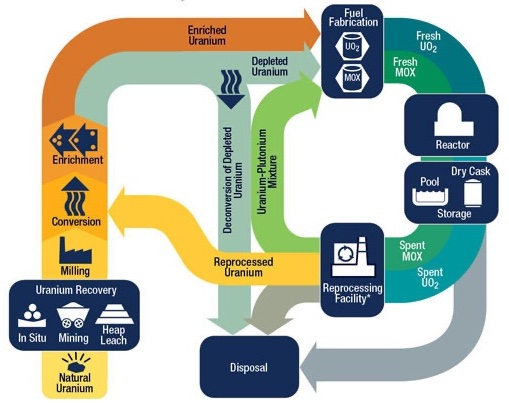
\includegraphics[width=0.8\textwidth]{./Figures/NRCFuelCycle.jpg}
\caption{Illustration of the nuclear fuel cycle (US Nuclear Regulatory Commission)}
\label{Fig:kinetics_nuclearFuelCycle}
\end{center}
\end{figure}

Before going into the analysis of the reactor, it is helpful to zoom out to the big picture of how the entire nuclear fuel cycle functions. This is depicted in Fig.~\ref{Fig:kinetics_nuclearFuelCycle}.

Before going into details, there are two primary types of fuel cycles in use. The US uses a once-through fuel cycle where fuel is put into a reactor, burned, and then disposed of as waste. France and Japan, on the other hand, perform fuel recycling, extracting the plutonium and blending it with uranium fuel to make mixed-oxide or MOX fuel assemblies that are then put back into reactors for additional burnup. 

The advantages of recycling is that it has a greater resource utilization and reduces the quantity of spent nuclear fuel that must be managed. The disadvantage is this comes at an increased cost, as mining uranium is inexpensive. Second, there is an increased risk of diversion of weapons usable materials. While reactor grade plutonium contains too much $^{240}$Pu to be an ideal nuclear explosive and is not the most attractive route for a nation state to pursue, it is nonetheless possible to use it for that purpose. This increased risk must be offset by increased costs to minimize the possibilities of such fuel diversions.

The once-through nuclear fuel cycle consists of the following major steps:
\begin{enumerate}
  \item Mining -- uranium is obtained by extracting it from ores underground resources. Like all mining, this is a polluting industry and is arguably the most environmentally damaging part of the nuclear fuel cycle. The argument in favor is because of the energy density of nuclear fuels, we require less mining than other energy sources.
  \item Milling -- the raw uranium ore must be extracted and comes in the composition of U$_3$O$_8$, which is sometimes called yellowcake. 
  \item Conversion -- in the US, fuel must be enriched and U$_3$O$_8$ is not a chemical form that permits this. We convert it into UF$_6$, which readily enters a gaseous phase.
  \item Enrichment -- the gaseous UF$_6$ is put into fast moving centrifuges. Because of the small mass differential between $^{235}$U and $^{238}$ the centrifugal forces preferentially push one isotope out more than other. The stock is moved through a series of such centrifuges until a desired enrichment (usually a few percent) is reached.
  \item Fuel Fabrication -- the enriched UF$_6$ is converted into ceramic UO$_2$ and sintered into pellets and sealed into fuel cladding tubes. These fuel rods are then put into bundles or assembles that are delivered to a power plant.
  \item Reactor -- the fuel is put into the reactor and is used to cause fission, producing thermal and then electrical energy. A typical fuel assembly resides in the reactor between 3-6 years.
  \item Onsite Storage -- once the fuel is sufficiently depleted it is moved out of the reactor for storage. Because of the large inventory of fission products, the fuel continues to generate a large amount of heat because of radioactive decay that must be removed. This is done by placing them into a spent fuel pool where the fuel assembly resides for several years. Once the radioactive inventory has decreased enough, the fuel is moved out of the pool and placed in dry casks that are cooled with air.
  \item Long-term Repository -- while not yet in operation, the plan in the US is to move the fuel in the spent fuel casks into a long-term or permanent repository for final disposition.
\end{enumerate}
 
In a fuel-recycle scenario, sometime after the fuel is removed from the reactor, it is sent to a reprocessing facility where it is chemically dissolved and separated. The plutonium is extracted and then mixed with uranium to create fuel with enough reactivity to go back into a reactor. The recycling process produces waste that must similarly be disposed of, but the volume and radiotoxicity is much less. 

More advanced fuel cycles are currently being investigated that make use of fast reactors that are capable of burning up the fissionable (but not fissile) actinides with long half lives that account for much of the radiotoxicity on the 1,000 to 100,000 year timeframe. While the technology is theoretically in place, it has yet to be demonstrated in an economically competitive manner.

\subsection{Burnup and Conversion Ratio}

Zooming back into the reactor eventually, the fuel becomes too depleted to effectively sustain a chain reaction and must be removed from the reactor. This can be mitigated by reshuffling the fuel and mixing it with fresh fuel assemblies, but there are still limits. The limiting factor is not the availability of fuel per se, but rather the fuel experiences steady damage from the energetic fission fragments. Additionally, the buildup of these fragments changes the chemistry, leading to corrosive chemical interactions with the cladding. Also, some of the fission products are gases and these fill the sealed fuel-cladding tube and lead to an increase in internal pressure. As the fuel continues to burn up, its structural integrity diminishes and the probability of fuel failure increases with time. Therefore, fuel inventory concerns aside, it is necessary to remove the fuel from the reactor after a few years lest the fuel rods begin to fail and leak fission products into the coolant.

We quantify the fuel exposure to neutrons with a quantity called \emph{burnup}, which is defined as
\begin{align}
  BU = \frac{\text{energy released from fission}}{\text{mass of the fissionable material}} .
\end{align}
Typically we express the energy in units of GWd (GigaWatt days), based on the thermal (not electrical) power of the reactor, and the units of mass as MTU, metric tons of uranium (excluding the mass of oxygen in the conventional UO$_2$ fuel). If different fissionable materials are used, then the mass needs to adjusted accordingly and sometimes the denominator is quoted as mass of heavy metal. Further, the mass of fissionable material typically includes all isotopes, not just, for example, the fissile $^{235}$U.

Typical end-of-life burnups for conventional UO$_2$ fuel is between 30 to 40 GWd/MTU. In recent years, there has been considerable effort to developing fuel capable of handling higher burnup, up to around 60 GWd/MTU, which means they can stay in the reactor longer and more energy can be extracted per unit mass. Advanced reactors such as gas-cooled variants use spherical TRISO fuel kernels that are capable of even higher fuel burnups.

As mentioned, some of the fertile $^{238}$U in a reactor is converted into fissile plutonium isotopes. In a conventional reactor, the depletion of $^{235}$U cannot keep up with the creation of plutonium. However, it is possible to create more fuel than is burned in a \emph{breeder reactor}. For thermal reactors, we use a thorium-based cycle where the fertile $^{232}$Th captures neutrons and produces (after a couple $\beta^-$ decays) fissile $^{233}$U, which is the actual fuel. In fast reactors, we typically convert $^{238}$U into Pu isotopes in an external blanket that can then be extracted, chemically separated, and used to make more fuel for other reactors. In the early days of nuclear power, the known resources of uranium was thought to be much more limited than it actually is. Today, there is a large supply of economically mineable uranium resources such that the resource question is far less of an short or medium term concern. That said, there is still interest in thorium cycles or fast reactors, but these are driven by other factors rather than long-term uranium resources.

Regardless of whether the intent is to breed new fuel, some will be produced and this quantity is called the \emph{conversion ratio}. This is
\begin{align}
  CR = \frac{\text{production rate of fissile atoms}}{\text{consumption rate of fissile atoms}} .
\end{align}
In a conventional reactor, the conversion ratio is less than one, i.e., the fuel is burned faster than it is produced. For a typical thermal power reactor, this conversion ratio is on the order of 0.5 to 0.6. In a breeder reactor, the conversion ratio is greater than one and is then usually called the \emph{breeding ratio}.




\subsection{Depletion Equations} \label{Sec:kinetics_fuelDepletionEquations}

Analyzing the depletion of the reactor is actually a very complicated process. Modern methods typically consider every reaction pathway and fission product individually, considering their radioactive decay. This is done by solving the rate equations including depletion and production, which is a series of first-order ordinary differential equations in each spatial region that depends on the local scalar flux $\phi(\pos,t)$. 

The general form of the rate equation in a reactor for isotope $i$ with concentration $N_i$ is
\begin{align}
  \frac{dN_i}{dt} &= 
  \underbrace{\sum_j \lambda_{ji} N_j(t) }_{\parbox{2.25cm}{\scriptsize rate isotope $i$ is produced from radioactive decay of all isotopes $j$}}
  + \underbrace{\sum_g \sum_j \gamma_{ji} \sigma_{f,g,j} \phi_g(t) N_j(t)}_{\parbox{3.5cm}{\scriptsize rate isotope $i$ is produced from fission from all fissionable isotopes $j$}}
  + \underbrace{\sum_g \sum_j \sigma_{g,ji} \phi_g(t) N_j(t)}_{\parbox{2.75cm}{\scriptsize rate isotope $i$ is produced from all non-fission nuclear reactions with isotopes $j$}} \nonumber \\*
  &- \underbrace{\sum_g \sum_x \sigma_{x,g,i} \phi_g(t) N_i(t)}_{\parbox{3cm}{\scriptsize rate isotope $i$ is removed because of all nuclear reactions $x$}}
  - \underbrace{\lambda_i N_i(t) }_{\parbox{1.75cm}{\scriptsize rate isotope $i$ is removed by radioactive decay}}.
\end{align}
Here
\begin{align}
  \lambda_{ji} &= \text{decay constant for isotope $j$ decaying to isotope $i$},  \nonumber \\
  \gamma_{ji}  &= \text{fission product yield for isotope $i$ from fissionable nucleus $j$}, \nonumber \\
  \sigma_{g,ji}  &= \text{reaction cross section for conversion from isotope $j$ into $i$ for energy group $g$}, \nonumber \\
  \sigma_{x,g,i} &= \text{cross section for reaction $x$ of isotope $i$ for energy group $g$}, \nonumber \\
  \lambda_i    &= \text{decay constant for isotope $i$ (for all decays)}. \nonumber 
\end{align}
An equation is written down for each isotope $i$. These equations can then be formed into a linear system as
\begin{align}
  \frac{d\mathbf{N}}{dt} = \mathbf{A}(t) \mathbf{N}(t) ,
\end{align}
where the coefficient matrix $\mathbf{A}$ depends on both the nuclear data and the local scalar flux $\phi(t)$, which carries the time dependence of the matrix.






\subsection{Burnup Flux Spectrum}

The depletion equations require knowledge of the reactor scalar flux within each region. Over the course of performing reactor analyses, we obtained several fluxes for various energy and spatial resolutions and we need to find an appropriate one to use. A typical process involves obtaining the leakage-corrected spectrum at the reflected assembly level, i.e., not using the full core nodal diffusion calculations, by using the $B_1$ spectra with the finely resolved, in both space and energy, transport fluxes that are scaled to the reactor power. The general process goes as follows:
\begin{enumerate}
  \item use the $B_1$ flux spectrum to rebalance the coarse-group assembly transport calculated fluxes;
  \item expand the coarse group flux spectra with the pin-level fine-group transport spectra;
  \item scale the fluxes to the reactor power.
\end{enumerate}

The first step is to perform the rebalance with the $B_1$ spectra for the homogenized assembly. As with the process to determine the few-group constants for the nodal diffusion calculations, the $B_1$ calculation adjusts the infinitely reflected assembly transport spectrum to account for the fact that in an actual reactor there must be a balance from either outflow (for a supercritical infinitely reflected assembly) or inflow (for a subcritical one) of neutrons from neighboring assemblies.

We define $\phi_{B,g}$ as the $B_1$ infinite medium spectrum for fine energy group $g$ and $\phi_{I,c}$ to be the flux spectrum within spatial region $I$ and coarse energy group $c$ from the assembly transport calculation. The leakage-corrected coarse-group spectrum is
\begin{subequations}
\begin{align}
  \phi_{L,I,c} = \frac{ \phi_{B,c} }{ \overline{\phi}_c } \phi_{I,c}
\end{align}
Here
\begin{align}
  \phi_{B,c} &= \sum_{g \in c} \phi_{B,g} \\
  \overline{\phi}_c &= \dfrac{ \displaystyle\sum_I \phi_{I,c} V_I }{ \displaystyle\sum_I V_I } .
\end{align}
\end{subequations}

We then expand the coarse groups into the fine groups. We let $\phi_{i,g}$ be the fluxes in fine-spatial region $i$ and fine-energy group $g$ from the pin-level collision probability/response matrix transport calculations. We then obtain the fine leakage-corrected flux spectra as
\begin{align}
  \phi_{L,i,g} = \dfrac{ \phi_{L,I,c} V_I }{ \displaystyle\sum_{i' \in I} V_{i'} \sum_{g' \in c} \phi_{i',g'} } \phi_{i,g} .
\end{align}

The final step in the process is to scale these fluxes by the power level to obtain $\phi_{P,i,g}$, the scaled fine fluxes. This is done by using
\begin{subequations}
\begin{align}
  \phi_{P,i,g} = \left[ \dfrac{ P M_0 }{ \displaystyle\sum_{i \in F} V_i \overline{\phi}_{L,i} \sum_j N_{j,i} \epsilon_j \overline{\sigma}_{f,j,i}  } \right] \phi_{L,i,g} ,
\end{align}
where
\begin{align}
  P &= \text{power density in units of watts per gram of fissionable material},  \nonumber \\
  M_0  &= \text{initial (pre-burnup) mass of fissionable material in units of grams}, \nonumber \\
  V_i  &= \text{volume of region $i$ within fuel $F$ in cm$^3$}, \nonumber \\
  \overline{\phi}_{L,i} &= \text{energy-integrated, leakage-corrected flux spectrum in region $i$ in cm$^{-2}$ s$^{-1}$}, \nonumber \\
  j    &= \text{index for fissionable isotope}, \nonumber \\
  N_{j,i} &= \text{atomic density of fissionable isotope $j$ within region $i$ in $10^{24}$ cm$^{-3}$}, \nonumber \\
  \epsilon_j &= \text{energy release per fission in Watt-seconds per fission}, \nonumber \\
  \overline{\sigma}_{f,j,i}    &= \text{spectrum-averaged fission cross section for isotope $j$ in $10^{-24}$ cm$^2$}. \nonumber 
\end{align}
The initial fissionable mass is calculated by
\begin{align}
  M_0 = \sum_{i \in F} V_i \sum_j N_{0,j,i} m_j ,
\end{align}
where $N_{0,j,i}$ is the initial (pre-burnup) atomic density in units of atoms per cm$^{3}$ times the mass $m_j$ in grams per atom. The energy-integrated leakage spectrum is calculated using
\begin{align}
  \overline{\phi}_{L,i} = \sum_g \phi_{L,i,g} .
\end{align}
The spectrum-averaged fission cross section is computed from
\begin{align}
  \overline{\sigma}_{f,j,i} &= \dfrac{ \displaystyle\sum_g \sigma_{f,j,i,g} \phi_{L,i,g} }{ \overline{\phi}_{L,i} } .
\end{align}
\end{subequations}

Once we have $\phi_P$ for each region and energy group, we then numerically solve the depletion equations. From here on in this section we drop the subscript $P$ as it is the implied flux spectrum in all depletion calculations.





\subsection{Predictor-Corrector Method}

If we assume that the scalar flux is constant over some time interval, i.e., a time step in a calculation $t_i \le t < t_{i+1}$, then this system has a solution as the matrix exponential,
\begin{align}
  \mathbf{N}(t) = \exp\left[ (t-t_i) \mathbf{A} \right] \mathbf{N}(t_i) , \quad t_i \le t < t_{i+1} ,
\end{align}
where $\mathbf{N}(t_i)$ is a known initial condition at $t = t_i$, the beginning of the interval. 

In practice this forward Euler scheme is not what is actually used. The complication that arises is similar to that of the fission product poisons in that the changes in local isotopics leads to a change in the local flux. This means that the depletion equations are non-linear and need to be solved numerically on a time grid that is fine enough to capture the temporal changes of the isotopic concentrations. 

The typical numerical scheme used is called the \emph{predictor-corrector method}. The idea is to break the reactor fueling cycle into a series of time steps that are sufficiently small to capture any changes in the reactor conditions. Typically, this means we need a relatively short time step or two to account for the buildup to the equilibrium states of the fission product poisons $^{135}$Xe and $^{149}$Sm every time the reactor changes its power level. Then, we need to take time steps of on the order of a few weeks to capture slower, long term fuel depletion and fertile conversion effects.

Suppose the isotopic compositions are known at the beginning of time step $t_i$ and given in a vector $\mathbf{N}(t_i)$ . We can then solve the neutron transport or diffusion equations using these componsitions with some numerical scheme to get the consistent scalar fluxes. We call these $\phi_1(t_i)$.

We then plug the scalar flux $\phi_1(t_i)$ into the system of rate equations and solve them at each position in the reactor to arrive at a \emph{prediction} of the new isotopic composition vector $\hat{\mathbf{N}}(t_i)$. We could use this prediction as the new isotopic compositions $\mathbf{N}(t_{i+1})$, but it turns out doing this, wile simple, would require taking very large time steps.

Instead, we use this new vector as input into the neutron transport and diffusion equation and solve for an updated scalar flux using the new compositions that we call $\phi_2(\pos,t_i)$. We then go back and compute a \emph{corrected} isotopic composition by using the average of the scalar fluxes,
\begin{align}
  \phi(t_i) = \frac{ \phi_1(t_i) + \phi_2(t_i) }{ 2 } ,
\end{align}
as the scalar flux to compute $\mathbf{N}(t_{i+1})$. We then use this as the initial condition of for the next time step. Because the core composition has changed, we then need to perform a criticality search after each time step based on changing control rod heights or soluble boron concentrations.

Note again that these equations must be solved for all locations in the reactor, so it can become a rather computationally taxing task for a large reactor with numerous fuel pins. Using the predictor-corrector method significantly improves the accuracy of the depletion solve over forward Euler and allows for taking much larger time steps than would be possible otherwise. More sophisticated methods exist, and finding better depletion solver techniques that balance accuracy versus computational costs remains an open area of study.

One thing worth mentioning is that the coefficients in the matrix $\mathbf{A}$ span several orders of magnitude. This implies we have phenomena that occur on timescales ranging from milliseconds to millions of years. It turns out that evaluating the matrix exponential is actually difficult in this case because of numerical precision issues. While this problem has not completely gone away, the last few decades have seen advances in numerical solution techniques capable of handing what we term stiff systems of differential equations, and the issue is far less acute than it used to be.




\end{document}
